% Options for packages loaded elsewhere
\PassOptionsToPackage{unicode}{hyperref}
\PassOptionsToPackage{hyphens}{url}
%
\documentclass[
]{book}
\usepackage{amsmath,amssymb}
\usepackage{iftex}
\ifPDFTeX
  \usepackage[T1]{fontenc}
  \usepackage[utf8]{inputenc}
  \usepackage{textcomp} % provide euro and other symbols
\else % if luatex or xetex
  \usepackage{unicode-math} % this also loads fontspec
  \defaultfontfeatures{Scale=MatchLowercase}
  \defaultfontfeatures[\rmfamily]{Ligatures=TeX,Scale=1}
\fi
\usepackage{lmodern}
\ifPDFTeX\else
  % xetex/luatex font selection
\fi
% Use upquote if available, for straight quotes in verbatim environments
\IfFileExists{upquote.sty}{\usepackage{upquote}}{}
\IfFileExists{microtype.sty}{% use microtype if available
  \usepackage[]{microtype}
  \UseMicrotypeSet[protrusion]{basicmath} % disable protrusion for tt fonts
}{}
\makeatletter
\@ifundefined{KOMAClassName}{% if non-KOMA class
  \IfFileExists{parskip.sty}{%
    \usepackage{parskip}
  }{% else
    \setlength{\parindent}{0pt}
    \setlength{\parskip}{6pt plus 2pt minus 1pt}}
}{% if KOMA class
  \KOMAoptions{parskip=half}}
\makeatother
\usepackage{xcolor}
\usepackage{color}
\usepackage{fancyvrb}
\newcommand{\VerbBar}{|}
\newcommand{\VERB}{\Verb[commandchars=\\\{\}]}
\DefineVerbatimEnvironment{Highlighting}{Verbatim}{commandchars=\\\{\}}
% Add ',fontsize=\small' for more characters per line
\usepackage{framed}
\definecolor{shadecolor}{RGB}{248,248,248}
\newenvironment{Shaded}{\begin{snugshade}}{\end{snugshade}}
\newcommand{\AlertTok}[1]{\textcolor[rgb]{0.94,0.16,0.16}{#1}}
\newcommand{\AnnotationTok}[1]{\textcolor[rgb]{0.56,0.35,0.01}{\textbf{\textit{#1}}}}
\newcommand{\AttributeTok}[1]{\textcolor[rgb]{0.13,0.29,0.53}{#1}}
\newcommand{\BaseNTok}[1]{\textcolor[rgb]{0.00,0.00,0.81}{#1}}
\newcommand{\BuiltInTok}[1]{#1}
\newcommand{\CharTok}[1]{\textcolor[rgb]{0.31,0.60,0.02}{#1}}
\newcommand{\CommentTok}[1]{\textcolor[rgb]{0.56,0.35,0.01}{\textit{#1}}}
\newcommand{\CommentVarTok}[1]{\textcolor[rgb]{0.56,0.35,0.01}{\textbf{\textit{#1}}}}
\newcommand{\ConstantTok}[1]{\textcolor[rgb]{0.56,0.35,0.01}{#1}}
\newcommand{\ControlFlowTok}[1]{\textcolor[rgb]{0.13,0.29,0.53}{\textbf{#1}}}
\newcommand{\DataTypeTok}[1]{\textcolor[rgb]{0.13,0.29,0.53}{#1}}
\newcommand{\DecValTok}[1]{\textcolor[rgb]{0.00,0.00,0.81}{#1}}
\newcommand{\DocumentationTok}[1]{\textcolor[rgb]{0.56,0.35,0.01}{\textbf{\textit{#1}}}}
\newcommand{\ErrorTok}[1]{\textcolor[rgb]{0.64,0.00,0.00}{\textbf{#1}}}
\newcommand{\ExtensionTok}[1]{#1}
\newcommand{\FloatTok}[1]{\textcolor[rgb]{0.00,0.00,0.81}{#1}}
\newcommand{\FunctionTok}[1]{\textcolor[rgb]{0.13,0.29,0.53}{\textbf{#1}}}
\newcommand{\ImportTok}[1]{#1}
\newcommand{\InformationTok}[1]{\textcolor[rgb]{0.56,0.35,0.01}{\textbf{\textit{#1}}}}
\newcommand{\KeywordTok}[1]{\textcolor[rgb]{0.13,0.29,0.53}{\textbf{#1}}}
\newcommand{\NormalTok}[1]{#1}
\newcommand{\OperatorTok}[1]{\textcolor[rgb]{0.81,0.36,0.00}{\textbf{#1}}}
\newcommand{\OtherTok}[1]{\textcolor[rgb]{0.56,0.35,0.01}{#1}}
\newcommand{\PreprocessorTok}[1]{\textcolor[rgb]{0.56,0.35,0.01}{\textit{#1}}}
\newcommand{\RegionMarkerTok}[1]{#1}
\newcommand{\SpecialCharTok}[1]{\textcolor[rgb]{0.81,0.36,0.00}{\textbf{#1}}}
\newcommand{\SpecialStringTok}[1]{\textcolor[rgb]{0.31,0.60,0.02}{#1}}
\newcommand{\StringTok}[1]{\textcolor[rgb]{0.31,0.60,0.02}{#1}}
\newcommand{\VariableTok}[1]{\textcolor[rgb]{0.00,0.00,0.00}{#1}}
\newcommand{\VerbatimStringTok}[1]{\textcolor[rgb]{0.31,0.60,0.02}{#1}}
\newcommand{\WarningTok}[1]{\textcolor[rgb]{0.56,0.35,0.01}{\textbf{\textit{#1}}}}
\usepackage{longtable,booktabs,array}
\usepackage{calc} % for calculating minipage widths
% Correct order of tables after \paragraph or \subparagraph
\usepackage{etoolbox}
\makeatletter
\patchcmd\longtable{\par}{\if@noskipsec\mbox{}\fi\par}{}{}
\makeatother
% Allow footnotes in longtable head/foot
\IfFileExists{footnotehyper.sty}{\usepackage{footnotehyper}}{\usepackage{footnote}}
\makesavenoteenv{longtable}
\usepackage{graphicx}
\makeatletter
\def\maxwidth{\ifdim\Gin@nat@width>\linewidth\linewidth\else\Gin@nat@width\fi}
\def\maxheight{\ifdim\Gin@nat@height>\textheight\textheight\else\Gin@nat@height\fi}
\makeatother
% Scale images if necessary, so that they will not overflow the page
% margins by default, and it is still possible to overwrite the defaults
% using explicit options in \includegraphics[width, height, ...]{}
\setkeys{Gin}{width=\maxwidth,height=\maxheight,keepaspectratio}
% Set default figure placement to htbp
\makeatletter
\def\fps@figure{htbp}
\makeatother
\usepackage{svg}
\setlength{\emergencystretch}{3em} % prevent overfull lines
\providecommand{\tightlist}{%
  \setlength{\itemsep}{0pt}\setlength{\parskip}{0pt}}
\setcounter{secnumdepth}{5}
\usepackage{booktabs}
\ifLuaTeX
  \usepackage{selnolig}  % disable illegal ligatures
\fi
\usepackage[]{natbib}
\bibliographystyle{plainnat}
\usepackage{bookmark}
\IfFileExists{xurl.sty}{\usepackage{xurl}}{} % add URL line breaks if available
\urlstyle{same}
\hypersetup{
  pdftitle={Research Process for Music Psychologists},
  pdfauthor={Daniel Yeom},
  hidelinks,
  pdfcreator={LaTeX via pandoc}}

\title{Research Process for Music Psychologists}
\usepackage{etoolbox}
\makeatletter
\providecommand{\subtitle}[1]{% add subtitle to \maketitle
  \apptocmd{\@title}{\par {\large #1 \par}}{}{}
}
\makeatother
\subtitle{R version}
\author{Daniel Yeom}
\date{2025-02-07}

\begin{document}
\maketitle

{
\setcounter{tocdepth}{1}
\tableofcontents
}
\chapter{Preface}\label{preface}

This is an R adaptation of the statistics content from a subject called Research Process for Music Psychologists (MUSI90252). The subject is an overview of research methods for Masters and PhD students in music psychology at the University of Melbourne.

\textbf{The general idea}

The subject's statistics material was originally written for Jamovi, given its ease of use and impressive functionality, but we have also encouraged any quantitative-oriented students to consider learning R in the long term. With that in mind, by and large the content is exactly the same as the Jamovi-focused content in the Canvas shell, except:

\begin{itemize}
\tightlist
\item
  Some commentary has either been added or removed for R-specific material (e.g.~information on functions).
\item
  Embedded content, such as that in Module 7, is not available here (but is Jamovi-specific anyway).
\item
  Some content has been reorganised in a minor way because of how R outputs things compared to Jamovi.
\item
  The first chapter is a very (\emph{very}) brief overview of how to use core R and tidyverse functions.
\end{itemize}

The R version of the RPMP content is therefore fairly different to the regular Jamovi version, by virtue of the fact that even though Jamovi is built on R it isn't necessarily built with R users in mind. Rather, Jamovi is built for users of SPSS and other platforms who may be used to a point and click approach. To clarify, there's nothing wrong with this at all - I actually think this is a great thing, and I believe one of Jamovi's greatest strengths is how easy it is to use. At the same time, for the budding R-using music psychologist - at least for RPMP - it means that the same procedures in R work a little differently to how they function in Jamovi. It's for this reason that the R adaptation of the MUSI90252 content has been written with one key principle in mind: \emph{parity with Jamovi}. R can and will do so much more than what is presented in this book, but again, the subject was originally designed with Jamovi users in mind.

\part{Introduction}\label{part-introduction}

\chapter{A very brief introduction to R}\label{intro-to-R}

This chapter is not meant to be an exhaustive be-all end-all to how to use R. It will only go through enough to complete RPMP's content. It will, however, introduce a couple of things that I think make for good starting habits using R - which is never a bad thing!

In general, I am a huge proponent of the `tidy' workflow of data analysis. While it was originally designed for data science in mind, I think it's a valuable model for psychological science as well:

\begin{center}\includegraphics{https://d33wubrfki0l68.cloudfront.net/e5bf2a8f4c787a12facbc0b4191fc82bd192f4c5/4e5d2/diagrams/data-science-model} \end{center}

The original subject was written with this workflow broadly in mind, although it wasn't intended to follow this closely (only to bring awareness to the general idea of modelling). For a far more comprehensive and rigorous overview of how to program in R, there is no better guide than \emph{R 4 Data Science} (R4DS) by Hadley Wickham: \url{https://r4ds.had.co.nz/}.

\section{Basic syntax}\label{R-syntax}

\subsection{Operators}\label{operators}

We can do basic maths in R using the following symbols:

\begin{itemize}
\item
  Addition: \texttt{+}
\item
  Subtraction: \texttt{-}
\item
  Multiplication: \texttt{*}
\item
  Division: \texttt{/}
\item
  Exponentiation: \texttt{\^{}}
\end{itemize}

\begin{Shaded}
\begin{Highlighting}[]
\CommentTok{\# Addition and subtraction}
\DecValTok{5} \SpecialCharTok{+} \DecValTok{2}
\end{Highlighting}
\end{Shaded}

\begin{verbatim}
## [1] 7
\end{verbatim}

\begin{Shaded}
\begin{Highlighting}[]
\DecValTok{6} \SpecialCharTok{{-}} \DecValTok{3}
\end{Highlighting}
\end{Shaded}

\begin{verbatim}
## [1] 3
\end{verbatim}

\begin{Shaded}
\begin{Highlighting}[]
\CommentTok{\# Multiplication and division}
\DecValTok{2} \SpecialCharTok{*} \DecValTok{5}
\end{Highlighting}
\end{Shaded}

\begin{verbatim}
## [1] 10
\end{verbatim}

\begin{Shaded}
\begin{Highlighting}[]
\DecValTok{24}\SpecialCharTok{/}\DecValTok{6}
\end{Highlighting}
\end{Shaded}

\begin{verbatim}
## [1] 4
\end{verbatim}

R will recognise brackets and perform calculations appropriately, following BEDMAS. As you normally would with a written equation, R will perform calculations left to right.

\begin{Shaded}
\begin{Highlighting}[]
\NormalTok{(}\DecValTok{6} \SpecialCharTok{+} \DecValTok{2}\NormalTok{) }\SpecialCharTok{*} \DecValTok{3}\SpecialCharTok{/}\DecValTok{4}
\end{Highlighting}
\end{Shaded}

\begin{verbatim}
## [1] 6
\end{verbatim}

\subsection{Assignment and naming}\label{assignment-and-naming}

When you type something in R, you almost always have the option of \emph{assigning} that value to a variable to give it a name. In R, assigning values/strings etc. to variables is slightly different to other programming languages. Instead of using equals signs, we use a left arrow \texttt{\textless{}-} for assignment. For example:

\begin{Shaded}
\begin{Highlighting}[]
\CommentTok{\# Use this}
\NormalTok{x }\OtherTok{\textless{}{-}} \DecValTok{5}

\CommentTok{\# This works but isn\textquotesingle{}t preferred }
\NormalTok{x }\OtherTok{=} \DecValTok{5}
\end{Highlighting}
\end{Shaded}

When it comes to naming variables and the like, the easiest/most readable way for most people is to separate words using an underscore. e.g.

\begin{Shaded}
\begin{Highlighting}[]
\CommentTok{\# this is preferred}
\NormalTok{variable\_name}

\CommentTok{\# this is also very common}
\NormalTok{variable.name}

\CommentTok{\# sentence case is also sometimes used}
\NormalTok{VariableName}

\CommentTok{\# no spaces are allowed}
\NormalTok{variable name }\CommentTok{\# This will give you an error}

\CommentTok{\# some heathens use camel case}
\NormalTok{variableName}
\end{Highlighting}
\end{Shaded}

To view what has been assigned to a variable, you can simply write the variable name:

\begin{Shaded}
\begin{Highlighting}[]
\CommentTok{\# This is the variable we named earlier}
\NormalTok{x}
\end{Highlighting}
\end{Shaded}

\begin{verbatim}
## [1] 5
\end{verbatim}

\subsection{Variable types}\label{variable-types}

Like many programming languages, R works by manipulating different types of variables. Knowing how to work with these different variables is fairly essential to using R, so here is a brief overview.

First, we have our most basic classes of variables. The first is \textbf{numeric}:

\begin{Shaded}
\begin{Highlighting}[]
\NormalTok{var\_a }\OtherTok{\textless{}{-}} \FloatTok{5.25}
\NormalTok{var\_a}
\end{Highlighting}
\end{Shaded}

\begin{verbatim}
## [1] 5.25
\end{verbatim}

A special form of a numeric variable is an \textbf{integer} variable, which is used for whole numbers.

\begin{Shaded}
\begin{Highlighting}[]
\NormalTok{var\_b }\OtherTok{\textless{}{-}} \DecValTok{6}
\NormalTok{var\_b}
\end{Highlighting}
\end{Shaded}

\begin{verbatim}
## [1] 6
\end{verbatim}

The second is \textbf{character}, which is used for text (or strings in programming language). Characters must be enclosed with speech marks:

\begin{Shaded}
\begin{Highlighting}[]
\NormalTok{var\_c }\OtherTok{\textless{}{-}} \StringTok{"This is a string"}
\NormalTok{var\_c}
\end{Highlighting}
\end{Shaded}

\begin{verbatim}
## [1] "This is a string"
\end{verbatim}

Finally, we have \textbf{logical} variables, which can take on the form of \texttt{TRUE} or \texttt{FALSE}. \texttt{TRUE} and \texttt{FALSE} (or alternatively \texttt{T} or \texttt{F}) are special values in R that, as their names suggest, are used to indicate when a certain value is true or false.

\begin{Shaded}
\begin{Highlighting}[]
\NormalTok{var\_d }\OtherTok{\textless{}{-}} \ConstantTok{TRUE}
\NormalTok{var\_d}
\end{Highlighting}
\end{Shaded}

\begin{verbatim}
## [1] TRUE
\end{verbatim}

\section{Data structures}\label{data-structures}

Of course, in R we don't work with single values (often). We instead work with larger data structures. While there are a number of data structures in R, by and large the main one we will work with are \textbf{data frames.}

\subsection{Vectors}\label{vectors}

Vectors are extremely important in R: so much so that many functions are what we call \emph{vectorised}, meaning that they operate over vectors. Vectors are a data structure that provide an ordered list of values of the same type. Vectors can contain multiple numbers, strings or logical values, as an example.

To create a vector, the \texttt{c()} function is used. Below is a vector containing 5 numbers:

\begin{Shaded}
\begin{Highlighting}[]
\NormalTok{vector\_a }\OtherTok{\textless{}{-}} \FunctionTok{c}\NormalTok{(}\DecValTok{4}\NormalTok{, }\DecValTok{1}\NormalTok{, }\DecValTok{6}\NormalTok{, }\DecValTok{2}\NormalTok{, }\DecValTok{3}\NormalTok{)}

\NormalTok{vector\_a}
\end{Highlighting}
\end{Shaded}

\begin{verbatim}
## [1] 4 1 6 2 3
\end{verbatim}

Each value in the vector has an \textbf{index}, which denotes its position in the vector starting from 1. We can pull values from vectors by using square brackets, \texttt{{[}{]}}. We give R the name of the vector, followed by the index of the value we want. Let us pull the number 1, for instance, which has an index of 2 (as it is 2nd in the vector):

\begin{Shaded}
\begin{Highlighting}[]
\NormalTok{vector\_a[}\DecValTok{2}\NormalTok{]}
\end{Highlighting}
\end{Shaded}

\begin{verbatim}
## [1] 1
\end{verbatim}

To subset multiple values, we can simply give a vector of indices within the square brackets. For example, let's say we want to pull values from indices 2-4. This means that our output should be 1, 6 and 2. We can create a vector corresponding to the indices that we want (\texttt{c(2,\ 3,\ 4)}), and give this to the square brackets for subsetting.

\begin{Shaded}
\begin{Highlighting}[]
\NormalTok{vector\_a[}\FunctionTok{c}\NormalTok{(}\DecValTok{2}\NormalTok{, }\DecValTok{3}\NormalTok{, }\DecValTok{4}\NormalTok{)]}
\end{Highlighting}
\end{Shaded}

\begin{verbatim}
## [1] 1 6 2
\end{verbatim}

But there's a neater trick here that R allows you to do. When placing a semicolon, \texttt{:}, between two numbers, R will create a vector of numbers between the two numbers you give. The below command, for example, will create a vector of integers between the numbers 2 and 7:

\begin{Shaded}
\begin{Highlighting}[]
\DecValTok{2}\SpecialCharTok{:}\DecValTok{7}
\end{Highlighting}
\end{Shaded}

\begin{verbatim}
## [1] 2 3 4 5 6 7
\end{verbatim}

We can use this to great effect by subsetting multiple values from a vector at once:

\begin{Shaded}
\begin{Highlighting}[]
\NormalTok{vector\_a[}\DecValTok{2}\SpecialCharTok{:}\DecValTok{4}\NormalTok{]}
\end{Highlighting}
\end{Shaded}

\begin{verbatim}
## [1] 1 6 2
\end{verbatim}

\subsection{Data frames}\label{dataframes}

Data frames are flexible, row-column structures that contain data. Data frames can essentially be thought of as several vectors joined together as columns.

R works best when data frames are in a \emph{tidy} format. In a tidy format:

\begin{itemize}
\tightlist
\item
  Each variable is its own column
\item
  Each observation (participant, object) is its own row
\item
  Each value is in its own cell.
\end{itemize}

\begin{figure}

{\centering \includegraphics{https://d33wubrfki0l68.cloudfront.net/6f1ddb544fc5c69a2478e444ab8112fb0eea23f8/91adc/images/tidy-1} 

}

\caption{Adapted from R4DS.}\label{fig:unnamed-chunk-21}
\end{figure}

Here is an example of a data frame in tidy format. Note how each column corresponds to a different variable, or piece of data that we're interested in. Each column is also clearly labelled, so it is clear what it represents. Each row corresponds to an observation (a single penguin, in this case). So, the first row represnts an Adelie penguin on Torgersen Island, with a bill length of 39.1mm etc etc.

\begin{Shaded}
\begin{Highlighting}[]
\FunctionTok{library}\NormalTok{(palmerpenguins)}
\NormalTok{penguins}
\end{Highlighting}
\end{Shaded}

\begin{verbatim}
## # A tibble: 344 x 8
##    species island    bill_length_mm bill_depth_mm flipper_length_mm body_mass_g
##    <fct>   <fct>              <dbl>         <dbl>             <int>       <int>
##  1 Adelie  Torgersen           39.1          18.7               181        3750
##  2 Adelie  Torgersen           39.5          17.4               186        3800
##  3 Adelie  Torgersen           40.3          18                 195        3250
##  4 Adelie  Torgersen           NA            NA                  NA          NA
##  5 Adelie  Torgersen           36.7          19.3               193        3450
##  6 Adelie  Torgersen           39.3          20.6               190        3650
##  7 Adelie  Torgersen           38.9          17.8               181        3625
##  8 Adelie  Torgersen           39.2          19.6               195        4675
##  9 Adelie  Torgersen           34.1          18.1               193        3475
## 10 Adelie  Torgersen           42            20.2               190        4250
## # i 334 more rows
## # i 2 more variables: sex <fct>, year <int>
\end{verbatim}

For the purposes of RPMP you won't need to create any data frames, but you will need to know how to read files in and work with them.

With data frames, there are a number of functions in base R that allow us to do certain operations. These will be super useful in a range of scenarios.

First, it helps to understand that data frames are (conceptually) like matrices, in that they have rows and columns that are indexed. We can therefore pull out bits of information by the row or column index (i.e.~number) using R. To do so, we can use the format \texttt{name{[}row,\ column{]}}. \texttt{name} in this instance is the name of our data frame, while \texttt{row} and \texttt{column} are the row and column numbers we want respectively. For example, let us take the cell corresponding to the first row and the first column:

\begin{Shaded}
\begin{Highlighting}[]
\NormalTok{penguins[}\DecValTok{1}\NormalTok{,}\DecValTok{1}\NormalTok{]}
\end{Highlighting}
\end{Shaded}

\begin{verbatim}
## # A tibble: 1 x 1
##   species
##   <fct>  
## 1 Adelie
\end{verbatim}

Or, the cell in row 3, column 4:

\begin{Shaded}
\begin{Highlighting}[]
\NormalTok{penguins[}\DecValTok{3}\NormalTok{,}\DecValTok{4}\NormalTok{]}
\end{Highlighting}
\end{Shaded}

\begin{verbatim}
## # A tibble: 1 x 1
##   bill_depth_mm
##           <dbl>
## 1            18
\end{verbatim}

We can pull out whole rows or columns by simply leaving the number blank. If we want all values in a row, we do not specify a column and vice versa. For example, let us take all of row 1 from the \texttt{penguins} dataset:

\begin{Shaded}
\begin{Highlighting}[]
\NormalTok{penguins[}\DecValTok{1}\NormalTok{,]}
\end{Highlighting}
\end{Shaded}

\begin{verbatim}
## # A tibble: 1 x 8
##   species island    bill_length_mm bill_depth_mm flipper_length_mm body_mass_g
##   <fct>   <fct>              <dbl>         <dbl>             <int>       <int>
## 1 Adelie  Torgersen           39.1          18.7               181        3750
## # i 2 more variables: sex <fct>, year <int>
\end{verbatim}

Or let's take all of the species column only, which is column 1:

\begin{Shaded}
\begin{Highlighting}[]
\NormalTok{penguins[,}\DecValTok{1}\NormalTok{]}
\end{Highlighting}
\end{Shaded}

\begin{verbatim}
## # A tibble: 344 x 1
##    species
##    <fct>  
##  1 Adelie 
##  2 Adelie 
##  3 Adelie 
##  4 Adelie 
##  5 Adelie 
##  6 Adelie 
##  7 Adelie 
##  8 Adelie 
##  9 Adelie 
## 10 Adelie 
## # i 334 more rows
\end{verbatim}

The above operation actually can be done another way in R, and perhaps a way that is more intuitive. With data frames, we can grab individual columns using the \texttt{\$} operator, followed by the column's \emph{name}. This lets us grab columns by their name.

\begin{Shaded}
\begin{Highlighting}[]
\NormalTok{penguins}\SpecialCharTok{$}\NormalTok{species}
\end{Highlighting}
\end{Shaded}

\begin{verbatim}
##   [1] Adelie    Adelie    Adelie    Adelie    Adelie    Adelie    Adelie   
##   [8] Adelie    Adelie    Adelie    Adelie    Adelie    Adelie    Adelie   
##  [15] Adelie    Adelie    Adelie    Adelie    Adelie    Adelie    Adelie   
##  [22] Adelie    Adelie    Adelie    Adelie    Adelie    Adelie    Adelie   
##  [29] Adelie    Adelie    Adelie    Adelie    Adelie    Adelie    Adelie   
##  [36] Adelie    Adelie    Adelie    Adelie    Adelie    Adelie    Adelie   
##  [43] Adelie    Adelie    Adelie    Adelie    Adelie    Adelie    Adelie   
##  [50] Adelie    Adelie    Adelie    Adelie    Adelie    Adelie    Adelie   
##  [57] Adelie    Adelie    Adelie    Adelie    Adelie    Adelie    Adelie   
##  [64] Adelie    Adelie    Adelie    Adelie    Adelie    Adelie    Adelie   
##  [71] Adelie    Adelie    Adelie    Adelie    Adelie    Adelie    Adelie   
##  [78] Adelie    Adelie    Adelie    Adelie    Adelie    Adelie    Adelie   
##  [85] Adelie    Adelie    Adelie    Adelie    Adelie    Adelie    Adelie   
##  [92] Adelie    Adelie    Adelie    Adelie    Adelie    Adelie    Adelie   
##  [99] Adelie    Adelie    Adelie    Adelie    Adelie    Adelie    Adelie   
## [106] Adelie    Adelie    Adelie    Adelie    Adelie    Adelie    Adelie   
## [113] Adelie    Adelie    Adelie    Adelie    Adelie    Adelie    Adelie   
## [120] Adelie    Adelie    Adelie    Adelie    Adelie    Adelie    Adelie   
## [127] Adelie    Adelie    Adelie    Adelie    Adelie    Adelie    Adelie   
## [134] Adelie    Adelie    Adelie    Adelie    Adelie    Adelie    Adelie   
## [141] Adelie    Adelie    Adelie    Adelie    Adelie    Adelie    Adelie   
## [148] Adelie    Adelie    Adelie    Adelie    Adelie    Gentoo    Gentoo   
## [155] Gentoo    Gentoo    Gentoo    Gentoo    Gentoo    Gentoo    Gentoo   
## [162] Gentoo    Gentoo    Gentoo    Gentoo    Gentoo    Gentoo    Gentoo   
## [169] Gentoo    Gentoo    Gentoo    Gentoo    Gentoo    Gentoo    Gentoo   
## [176] Gentoo    Gentoo    Gentoo    Gentoo    Gentoo    Gentoo    Gentoo   
## [183] Gentoo    Gentoo    Gentoo    Gentoo    Gentoo    Gentoo    Gentoo   
## [190] Gentoo    Gentoo    Gentoo    Gentoo    Gentoo    Gentoo    Gentoo   
## [197] Gentoo    Gentoo    Gentoo    Gentoo    Gentoo    Gentoo    Gentoo   
## [204] Gentoo    Gentoo    Gentoo    Gentoo    Gentoo    Gentoo    Gentoo   
## [211] Gentoo    Gentoo    Gentoo    Gentoo    Gentoo    Gentoo    Gentoo   
## [218] Gentoo    Gentoo    Gentoo    Gentoo    Gentoo    Gentoo    Gentoo   
## [225] Gentoo    Gentoo    Gentoo    Gentoo    Gentoo    Gentoo    Gentoo   
## [232] Gentoo    Gentoo    Gentoo    Gentoo    Gentoo    Gentoo    Gentoo   
## [239] Gentoo    Gentoo    Gentoo    Gentoo    Gentoo    Gentoo    Gentoo   
## [246] Gentoo    Gentoo    Gentoo    Gentoo    Gentoo    Gentoo    Gentoo   
## [253] Gentoo    Gentoo    Gentoo    Gentoo    Gentoo    Gentoo    Gentoo   
## [260] Gentoo    Gentoo    Gentoo    Gentoo    Gentoo    Gentoo    Gentoo   
## [267] Gentoo    Gentoo    Gentoo    Gentoo    Gentoo    Gentoo    Gentoo   
## [274] Gentoo    Gentoo    Gentoo    Chinstrap Chinstrap Chinstrap Chinstrap
## [281] Chinstrap Chinstrap Chinstrap Chinstrap Chinstrap Chinstrap Chinstrap
## [288] Chinstrap Chinstrap Chinstrap Chinstrap Chinstrap Chinstrap Chinstrap
## [295] Chinstrap Chinstrap Chinstrap Chinstrap Chinstrap Chinstrap Chinstrap
## [302] Chinstrap Chinstrap Chinstrap Chinstrap Chinstrap Chinstrap Chinstrap
## [309] Chinstrap Chinstrap Chinstrap Chinstrap Chinstrap Chinstrap Chinstrap
## [316] Chinstrap Chinstrap Chinstrap Chinstrap Chinstrap Chinstrap Chinstrap
## [323] Chinstrap Chinstrap Chinstrap Chinstrap Chinstrap Chinstrap Chinstrap
## [330] Chinstrap Chinstrap Chinstrap Chinstrap Chinstrap Chinstrap Chinstrap
## [337] Chinstrap Chinstrap Chinstrap Chinstrap Chinstrap Chinstrap Chinstrap
## [344] Chinstrap
## Levels: Adelie Chinstrap Gentoo
\end{verbatim}

Note though that the output here is different; it simply returns a vector, while the \texttt{{[}row,column{]}} notation returns a data frame. Given that many functions in R rely on vectors, this notation is often useful.

Finally, if we want to select multiple rows or columns then we need to give vectors to the row and/or column arguments within the square brackets. This means that our semicolon notation will work here as well. For instance, let's say we want to get the first 6 rows of the dataset:

\begin{Shaded}
\begin{Highlighting}[]
\NormalTok{penguins[}\DecValTok{1}\SpecialCharTok{:}\DecValTok{6}\NormalTok{,]}
\end{Highlighting}
\end{Shaded}

\begin{verbatim}
## # A tibble: 6 x 8
##   species island    bill_length_mm bill_depth_mm flipper_length_mm body_mass_g
##   <fct>   <fct>              <dbl>         <dbl>             <int>       <int>
## 1 Adelie  Torgersen           39.1          18.7               181        3750
## 2 Adelie  Torgersen           39.5          17.4               186        3800
## 3 Adelie  Torgersen           40.3          18                 195        3250
## 4 Adelie  Torgersen           NA            NA                  NA          NA
## 5 Adelie  Torgersen           36.7          19.3               193        3450
## 6 Adelie  Torgersen           39.3          20.6               190        3650
## # i 2 more variables: sex <fct>, year <int>
\end{verbatim}

Or, columns 2 to 4:

\begin{Shaded}
\begin{Highlighting}[]
\NormalTok{penguins[,}\DecValTok{2}\SpecialCharTok{:}\DecValTok{4}\NormalTok{]}
\end{Highlighting}
\end{Shaded}

\begin{verbatim}
## # A tibble: 344 x 3
##    island    bill_length_mm bill_depth_mm
##    <fct>              <dbl>         <dbl>
##  1 Torgersen           39.1          18.7
##  2 Torgersen           39.5          17.4
##  3 Torgersen           40.3          18  
##  4 Torgersen           NA            NA  
##  5 Torgersen           36.7          19.3
##  6 Torgersen           39.3          20.6
##  7 Torgersen           38.9          17.8
##  8 Torgersen           39.2          19.6
##  9 Torgersen           34.1          18.1
## 10 Torgersen           42            20.2
## # i 334 more rows
\end{verbatim}

\section{Packages and functions}\label{packages-and-functions}

\subsection{Functions}\label{functions}

R works primarily with \textbf{functions}, which take one or more inputs and return an output. Functions in R are always defined in \texttt{name()} format, i.e.~the name of the function followed by brackets. Every function generally serves a very specific purpose, such as performing a specific calculation, manipulation of data or otherwise. Therefore, working with R requires us to use lots and lots of functions.

Most functions will have at least one, if not multiple \textbf{arguments.} Arguments define the options for a given function. For example, the \texttt{class()} function, which comes in base R, tells us the type of a variable. \texttt{class()} has one main argument, \texttt{x} - which is simply the name of the variable we want to know about. As an example, let us say we wanted to know what type of variable \texttt{var\_a} was. We could write the following:

\begin{Shaded}
\begin{Highlighting}[]
\FunctionTok{class}\NormalTok{(}\AttributeTok{x =}\NormalTok{ var\_a)}
\end{Highlighting}
\end{Shaded}

\begin{verbatim}
## [1] "numeric"
\end{verbatim}

More simply, because \texttt{class()} only has one argument we can optionally write:

\begin{Shaded}
\begin{Highlighting}[]
\FunctionTok{class}\NormalTok{(var\_a)}
\end{Highlighting}
\end{Shaded}

\begin{verbatim}
## [1] "numeric"
\end{verbatim}

Functions may either have mandatory or optional arguments. Mandatory arguments are ones that you need to provide in order for the function to run. Optional arguments are often defaults that can be changed if needed. Many functions in R will have multiple arguments that are typically a mix of both. A key point arises here though: functions in R define arguments in specific orders. In other words, R expects you to input arguments in specific orders unless you explicitly define each argument's value, as we did for the first instance of \texttt{class()}.

The easiest way to find out information about what a function does and the arguments it requires is to type a question mark, \texttt{?}, with the name of the function immediately afterwards. e.g.~

\begin{Shaded}
\begin{Highlighting}[]
\NormalTok{?class}
\end{Highlighting}
\end{Shaded}

A basic function is the \texttt{round()} function, which - as the name suggests - rounds a value you give it. \texttt{round()} has two arguments: \texttt{x}, which is the number or the name of an object we want to round, and \texttt{digits}, which specifies the number of digits we want to round to. \texttt{x} is a mandatory argument, but \texttt{digits} is optional and has a preset value of 0. Therefore, if we type in the following you can see what we get:

\begin{Shaded}
\begin{Highlighting}[]
\FunctionTok{round}\NormalTok{(}\FloatTok{4.326}\NormalTok{)}
\end{Highlighting}
\end{Shaded}

\begin{verbatim}
## [1] 4
\end{verbatim}

If we want to round to 2dp, for instance, we would need to explicitly define the \texttt{digits} argument and set it to a different value.

\begin{Shaded}
\begin{Highlighting}[]
\FunctionTok{round}\NormalTok{(}\FloatTok{4.326}\NormalTok{, }\AttributeTok{digits =} \DecValTok{2}\NormalTok{)}
\end{Highlighting}
\end{Shaded}

\begin{verbatim}
## [1] 4.33
\end{verbatim}

\subsection{Packages}\label{packages}

By default, R comes with \emph{lots} of functions, many of which will be used throughout this book. The beauty of R though is that its functionality is essentially limitless; its open-source nature and strong community mean that new functions and capabilities are regularly made for R. These new functions augment/extend what R is capable of doing, and are generally available in the form of \textbf{packages.} To provide a very simple explanation of what packages are, packages are a collection of code that provide extra functions in R. Some packages occassionally come with data too, such as the \texttt{palmerpenguins} package.

When you start a new R session, the first thing that you'll want to do is load the packages that you need to use.

For now, we'll load two packages for functions: \texttt{tidyverse} and \texttt{rstatix}. \texttt{tidyverse} is a huge package that contains a group of other packages designed for data manipulation, visualisation and cleaning. \texttt{rstatix} allows for simple statistical tests to be performed in an easy way. \texttt{palmerpenguins} comes with a dataset for practicing on. \texttt{palmerpenguins} loads a dataset named \texttt{penguins} that contains basic info on 3 species of penguins across 3 different islands.

To load a package, call the \texttt{library()} function and enter the name of the package in brackets:

\begin{Shaded}
\begin{Highlighting}[]
\FunctionTok{library}\NormalTok{(tidyverse)}
\end{Highlighting}
\end{Shaded}

\begin{verbatim}
## -- Attaching core tidyverse packages ------------------------ tidyverse 2.0.0 --
## v dplyr     1.1.4     v readr     2.1.5
## v forcats   1.0.0     v stringr   1.5.1
## v ggplot2   3.5.1     v tibble    3.2.1
## v lubridate 1.9.4     v tidyr     1.3.1
## v purrr     1.0.2     
## -- Conflicts ------------------------------------------ tidyverse_conflicts() --
## x dplyr::filter() masks stats::filter()
## x dplyr::lag()    masks stats::lag()
## i Use the conflicted package (<http://conflicted.r-lib.org/>) to force all conflicts to become errors
\end{verbatim}

\begin{Shaded}
\begin{Highlighting}[]
\FunctionTok{library}\NormalTok{(rstatix)}
\end{Highlighting}
\end{Shaded}

\begin{verbatim}
## 
## Attaching package: 'rstatix'
## 
## The following object is masked from 'package:stats':
## 
##     filter
\end{verbatim}

\begin{Shaded}
\begin{Highlighting}[]
\FunctionTok{library}\NormalTok{(palmerpenguins)}
\end{Highlighting}
\end{Shaded}

\subsection{Tidyverse}\label{tidyverse}

The tidyverse is a mega-collection of phenomenal packages that fundamentally change how to interface with R. The tidyverse provides packages for things like:

\begin{itemize}
\tightlist
\item
  Wrangling data
\item
  Reading and writing data
\item
  Making graphs
\item
  Tidying and reshaping data
\item
  Scraping the web
\end{itemize}

The tidyverse is probably the single most popular suite of packages for R because of the functionality it provides. All of the tidyverse packages are written in consistent syntax, generally use very easy language that has an emphasis on verbs (i.e.~you're telling R to \emph{do} something) and integrate seamlessly with each other and R. The tidyverse is a philosophy of R just as much as it is a suite of functions, and is part of what makes R so powerful today.

Many aspects of the tidyverse are reliant on the pipe operator, \texttt{\%\textgreater{}\%}. This basically tells R to take a dataframe or output and pass it onto a function that comes directly afterwards. Any function that takes a data frame as its first argument can (theoretically) be piped, meaning that we can chain strings of functions together in one run in a readable way. See the example below:

\begin{Shaded}
\begin{Highlighting}[]
\NormalTok{data }\SpecialCharTok{\%\textgreater{}\%}
  \FunctionTok{function\_1}\NormalTok{() }\SpecialCharTok{\%\textgreater{}\%}
  \FunctionTok{function\_2}\NormalTok{(}\AttributeTok{do =} \StringTok{"this"}\NormalTok{) }\SpecialCharTok{\%\textgreater{}\%}
  \FunctionTok{function\_3}\NormalTok{(}\AttributeTok{avoid =} \StringTok{"that"}\NormalTok{)}
\end{Highlighting}
\end{Shaded}

in the hypothetical example above, we first take \texttt{data}, and pass it to function 1. We then take the output of function 1 and pass that to function 2, which has the argument \texttt{do\ =\ "this"}. Afterwards, we take the output of function 2 and pass it to function 3.

There are a number of clear benefits to the tidyverse way of doing things. These include:

\begin{itemize}
\tightlist
\item
  Functions are generally stated as \emph{verbs}, which means that you're always \emph{doing} something with a function (and it's clear what that something is)
\item
  Piping avoids the cyclical hell of creating intermediate variables. Consider a non-tidyverse version of the code example above, written down below. This code is not only a bit of a pain to read, but is also clunky in that it generates several intermediate variables that aren't all that useful (a lot of the time).
\end{itemize}

\begin{Shaded}
\begin{Highlighting}[]
\NormalTok{output\_1 }\OtherTok{\textless{}{-}} \FunctionTok{function\_1}\NormalTok{(data)}
\NormalTok{output\_2 }\OtherTok{\textless{}{-}} \FunctionTok{function\_2}\NormalTok{(output\_1, }\AttributeTok{do =} \StringTok{"this"}\NormalTok{)}
\NormalTok{output\_3 }\OtherTok{\textless{}{-}} \FunctionTok{function\_3}\NormalTok{(output\_2, }\AttributeTok{avoid =} \StringTok{"that"}\NormalTok{)}
\end{Highlighting}
\end{Shaded}

\begin{itemize}
\tightlist
\item
  Piped code is generally quite easy to read.
\item
  \texttt{tidyverse} also provides a consistent syntax for \emph{other} packages! It provides a quasi-philosophy and style guide for developers to write their own packages to write `tidy' packages. \texttt{rstatix} is a great example of this.
\end{itemize}

Throughout this book you will see a lot of tidyverse!

\subsection{\texorpdfstring{The \texttt{here()} package}{The here() package}}\label{the-here-package}

Another staple bit of code you will see throughout RPMP is the \texttt{here} package. The official vignette for \texttt{here} summarises what this package does:

\begin{quote}
The \texttt{here} package enables easy file referencing by using the top-level directory of a file project to easily build file paths. This is in contrast to using \texttt{setwd()}, which is fragile and dependent on the way you order your files on your computer.
\end{quote}

Alternatively, read the below quote from R goddess Jenny Bryan:

\begin{quote}
If the first line of your \#rstats script is \texttt{setwd("C:\textbackslash{}Users\textbackslash{}jenny\textbackslash{}path\textbackslash{}that\textbackslash{}only\textbackslash{}I\textbackslash{}have")}, I will come into your lab and SET YOUR COMPUTER ON FIRE.
\end{quote}

In short, \texttt{here()} allows us to locate files in a \emph{relative} manner as opposed to an \emph{absolute} one. This is super super useful for sharing your code and data with other people, and ensuring that your scripts will run no matter where they are.

We won't get into project-oriented workflows for RPMP. However, imagine you have a folder structure like this:

\begin{verbatim}
|-code
|-----rpmp_week1.Rmd
|-data
|-----w1_dataset.csv
|-output
|-RPMP.rproj
\end{verbatim}

Normally, to locate a file on a disk you would generally have to give the entire pathway to that file. That could be something like \texttt{"C:\textbackslash{}Users\textbackslash{}Dan\textbackslash{}Documents\textbackslash{}Subjects\textbackslash{}RPMP\textbackslash{}data\textbackslash{}w1\_dataset.csv"} - which is immensely unwieldy if we want to read in data - and won't work the moment I give my script to someone else, as their folder structure could be completely different!

The alternative with here could be as simple as:

\begin{Shaded}
\begin{Highlighting}[]
\FunctionTok{here}\NormalTok{(}\StringTok{"data"}\NormalTok{, }\StringTok{"w1\_dataset.csv"}\NormalTok{)}
\end{Highlighting}
\end{Shaded}

This tells R that I'm looking for something \emph{here} in the data folder, specifically a file named \texttt{w1\_dataset.csv}. As long as the relative positions are correct - i.e.~the \texttt{.csv} file is in the \texttt{data} folder - R will know where to locate the file.

You will see a lot of \texttt{here()} in this version of the RPMP guide because as you may appreciate, there are a lot of data files stored in all manner of folders.

\section{Wrangling data with dplyr and others}\label{wrangling-data-with-dplyr-and-others}

\texttt{dplyr} is a package within the tidyverse for manipulating and wrangling data. \texttt{dplyr} is one of the most popular packages on R because it provides a suite of functions that are fairly essential to manipulating and working with data. Below is a brief overview of some of these functions, applied to the \texttt{penguins} dataset.

\subsection{\texorpdfstring{Selecting columns with \texttt{select()}}{Selecting columns with select()}}\label{selecting-columns-with-select}

\texttt{select()} lets you select the columns you want from a dataset. Simply specify the columns that you want by name. Below we take the species and island columns from the penguins dataset:

\begin{Shaded}
\begin{Highlighting}[]
\NormalTok{penguins }\SpecialCharTok{\%\textgreater{}\%}
  \FunctionTok{select}\NormalTok{(species, island)}
\end{Highlighting}
\end{Shaded}

\begin{verbatim}
## # A tibble: 344 x 2
##    species island   
##    <fct>   <fct>    
##  1 Adelie  Torgersen
##  2 Adelie  Torgersen
##  3 Adelie  Torgersen
##  4 Adelie  Torgersen
##  5 Adelie  Torgersen
##  6 Adelie  Torgersen
##  7 Adelie  Torgersen
##  8 Adelie  Torgersen
##  9 Adelie  Torgersen
## 10 Adelie  Torgersen
## # i 334 more rows
\end{verbatim}

You can select columns via a number of ways:

\begin{itemize}
\tightlist
\item
  Simply by name, e.g.~\texttt{select(species,\ island)}
\item
  By their \emph{index} or column number, e.g.~\texttt{select(1,\ 2)}

  \begin{itemize}
  \tightlist
  \item
    \texttt{select(1:4)} will select columns 1 to 4
  \item
    \texttt{select(-1)} will select the \emph{last} column
  \end{itemize}
\item
  By certain operator functions, such as \texttt{starts\_with()} and \texttt{ends\_with()}, e.g.~\texttt{ends\_with("mm")} will select all columns that end with ``mm''
\end{itemize}

Combinations of the above also work. Removing columns is simply done by adding a minus sign \texttt{-} in front of the arguments for select, and are compatible with all of the options above.

\subsection{\texorpdfstring{Filtering rows with \texttt{filter()}}{Filtering rows with filter()}}\label{filtering-rows-with-filter}

\texttt{filter()} selects the rows that you want based on a certain condition. Here, we specify the column that want to filter by and state the condition (\texttt{==} means equals to). We can filter on multiple conditions; for example, filtering Adelie penguins by the year 2007:

\begin{Shaded}
\begin{Highlighting}[]
\NormalTok{penguins }\SpecialCharTok{\%\textgreater{}\%}
  \FunctionTok{filter}\NormalTok{(year }\SpecialCharTok{==} \DecValTok{2007}\NormalTok{, species }\SpecialCharTok{==} \StringTok{"Adelie"}\NormalTok{)}
\end{Highlighting}
\end{Shaded}

\begin{verbatim}
## # A tibble: 50 x 8
##    species island    bill_length_mm bill_depth_mm flipper_length_mm body_mass_g
##    <fct>   <fct>              <dbl>         <dbl>             <int>       <int>
##  1 Adelie  Torgersen           39.1          18.7               181        3750
##  2 Adelie  Torgersen           39.5          17.4               186        3800
##  3 Adelie  Torgersen           40.3          18                 195        3250
##  4 Adelie  Torgersen           NA            NA                  NA          NA
##  5 Adelie  Torgersen           36.7          19.3               193        3450
##  6 Adelie  Torgersen           39.3          20.6               190        3650
##  7 Adelie  Torgersen           38.9          17.8               181        3625
##  8 Adelie  Torgersen           39.2          19.6               195        4675
##  9 Adelie  Torgersen           34.1          18.1               193        3475
## 10 Adelie  Torgersen           42            20.2               190        4250
## # i 40 more rows
## # i 2 more variables: sex <fct>, year <int>
\end{verbatim}

You can also choose to filter \emph{out} rows based on a condition by adding an exclamation mark in front of the column name.

\begin{Shaded}
\begin{Highlighting}[]
\NormalTok{penguins }\SpecialCharTok{\%\textgreater{}\%}
  \FunctionTok{filter}\NormalTok{(}\SpecialCharTok{!}\NormalTok{year }\SpecialCharTok{==} \DecValTok{2007}\NormalTok{)}
\end{Highlighting}
\end{Shaded}

\begin{verbatim}
## # A tibble: 234 x 8
##    species island bill_length_mm bill_depth_mm flipper_length_mm body_mass_g
##    <fct>   <fct>           <dbl>         <dbl>             <int>       <int>
##  1 Adelie  Biscoe           39.6          17.7               186        3500
##  2 Adelie  Biscoe           40.1          18.9               188        4300
##  3 Adelie  Biscoe           35            17.9               190        3450
##  4 Adelie  Biscoe           42            19.5               200        4050
##  5 Adelie  Biscoe           34.5          18.1               187        2900
##  6 Adelie  Biscoe           41.4          18.6               191        3700
##  7 Adelie  Biscoe           39            17.5               186        3550
##  8 Adelie  Biscoe           40.6          18.8               193        3800
##  9 Adelie  Biscoe           36.5          16.6               181        2850
## 10 Adelie  Biscoe           37.6          19.1               194        3750
## # i 224 more rows
## # i 2 more variables: sex <fct>, year <int>
\end{verbatim}

\texttt{drop\_na()} is another useful starting function that simply removes all rows with NA/empty cells. If you enter it as is then it will clean the entire dataset; if you specify a column then it will remove all rows with NAs in that column. Below is an example of a pipe using these functions - going from selecting columns to filtering rows and finally cleaning up the empty cells.

\begin{Shaded}
\begin{Highlighting}[]
\NormalTok{penguins }\SpecialCharTok{\%\textgreater{}\%}
  \FunctionTok{select}\NormalTok{(species, body\_mass\_g, year) }\SpecialCharTok{\%\textgreater{}\%}
  \FunctionTok{filter}\NormalTok{(year }\SpecialCharTok{==} \DecValTok{2009}\NormalTok{) }\SpecialCharTok{\%\textgreater{}\%}
  \FunctionTok{drop\_na}\NormalTok{()}
\end{Highlighting}
\end{Shaded}

\begin{verbatim}
## # A tibble: 119 x 3
##    species body_mass_g  year
##    <fct>         <int> <int>
##  1 Adelie         3725  2009
##  2 Adelie         4725  2009
##  3 Adelie         3075  2009
##  4 Adelie         4250  2009
##  5 Adelie         2925  2009
##  6 Adelie         3550  2009
##  7 Adelie         3750  2009
##  8 Adelie         3900  2009
##  9 Adelie         3175  2009
## 10 Adelie         4775  2009
## # i 109 more rows
\end{verbatim}

\subsection{\texorpdfstring{Creating new columns with \texttt{mutate()}}{Creating new columns with mutate()}}\label{creating-new-columns-with-mutate}

\texttt{mutate()} is a function that lets you create new columns. This can be extremely useful for operations like recoding variables and transforming them. The nice thing about \texttt{mutate()} is that you can do all manner of operations without touching your original data.

The basic workflow of \texttt{mutate()} looks like this:

\begin{Shaded}
\begin{Highlighting}[]
\NormalTok{data }\SpecialCharTok{\%\textgreater{}\%}
  \FunctionTok{mutate}\NormalTok{(}
    \AttributeTok{new\_column\_1 =} \FunctionTok{a\_function}\NormalTok{(...),}
    \AttributeTok{new\_column\_2 =} \FunctionTok{another\_function}\NormalTok{(...)}
\NormalTok{    )}
\end{Highlighting}
\end{Shaded}

This example code would create two new columns, named \texttt{new\_column\_1} and \texttt{new\_column\_2}, with their respective values being whatever the functions were. For example, in the \texttt{penguins} dataset we have a variable called \texttt{body\_mass\_g}, which is the body mass of each penguin in grams. If we wanted to convert this to kilograms, we would need to divide each penguin's value on this variable by 1000. \texttt{mutate()} makes this a piece of cake. Let's also chain a \texttt{select()} command to only show the following variables: species, island, body\_mass\_g and sex.

\begin{Shaded}
\begin{Highlighting}[]
\NormalTok{penguins }\SpecialCharTok{\%\textgreater{}\%}
  \FunctionTok{select}\NormalTok{(species, island, body\_mass\_g, sex) }\SpecialCharTok{\%\textgreater{}\%}
  \FunctionTok{mutate}\NormalTok{(}\AttributeTok{body\_mass\_kg =}\NormalTok{ body\_mass\_g}\SpecialCharTok{/}\DecValTok{1000}\NormalTok{)}
\end{Highlighting}
\end{Shaded}

\begin{verbatim}
## # A tibble: 344 x 5
##    species island    body_mass_g sex    body_mass_kg
##    <fct>   <fct>           <int> <fct>         <dbl>
##  1 Adelie  Torgersen        3750 male           3.75
##  2 Adelie  Torgersen        3800 female         3.8 
##  3 Adelie  Torgersen        3250 female         3.25
##  4 Adelie  Torgersen          NA <NA>          NA   
##  5 Adelie  Torgersen        3450 female         3.45
##  6 Adelie  Torgersen        3650 male           3.65
##  7 Adelie  Torgersen        3625 female         3.62
##  8 Adelie  Torgersen        4675 male           4.68
##  9 Adelie  Torgersen        3475 <NA>           3.48
## 10 Adelie  Torgersen        4250 <NA>           4.25
## # i 334 more rows
\end{verbatim}

You can see now that we have a new column called \texttt{body\_mass\_kg} that has our new transformed variable.

\texttt{mutate()} can also take functions (and likely will make up the majority of your use of it). For example, let's say that we want to make a variable that takes the natural logarithm of bill length (for whatever reason). We could do this as follows using the \texttt{log()} function within our \texttt{mutate()} call:

\begin{Shaded}
\begin{Highlighting}[]
\NormalTok{penguins }\SpecialCharTok{\%\textgreater{}\%}
  \FunctionTok{select}\NormalTok{(species, island, bill\_length\_mm, bill\_depth\_mm) }\SpecialCharTok{\%\textgreater{}\%}
  \FunctionTok{mutate}\NormalTok{(}\AttributeTok{bill\_length\_log =} \FunctionTok{log}\NormalTok{(bill\_length\_mm))}
\end{Highlighting}
\end{Shaded}

\begin{verbatim}
## # A tibble: 344 x 5
##    species island    bill_length_mm bill_depth_mm bill_length_log
##    <fct>   <fct>              <dbl>         <dbl>           <dbl>
##  1 Adelie  Torgersen           39.1          18.7            3.67
##  2 Adelie  Torgersen           39.5          17.4            3.68
##  3 Adelie  Torgersen           40.3          18              3.70
##  4 Adelie  Torgersen           NA            NA             NA   
##  5 Adelie  Torgersen           36.7          19.3            3.60
##  6 Adelie  Torgersen           39.3          20.6            3.67
##  7 Adelie  Torgersen           38.9          17.8            3.66
##  8 Adelie  Torgersen           39.2          19.6            3.67
##  9 Adelie  Torgersen           34.1          18.1            3.53
## 10 Adelie  Torgersen           42            20.2            3.74
## # i 334 more rows
\end{verbatim}

\subsection{\texorpdfstring{Summarising data with \texttt{summarise()} and \texttt{group\_by()}}{Summarising data with summarise() and group\_by()}}\label{summarising-data-with-summarise-and-group_by}

Finally, sometimes we will want to summarise data - for example, to calculate basic features such as descriptives or for plotting. To do that, we can use the function \texttt{summarise()} (or \texttt{summarize()} for American users).

\texttt{summarise()} works very similarly to \texttt{mutate()}.

\begin{Shaded}
\begin{Highlighting}[]
\NormalTok{data }\SpecialCharTok{\%\textgreater{}\%}
  \FunctionTok{summarise}\NormalTok{(}
    \AttributeTok{summary\_1 =} \FunctionTok{a\_function}\NormalTok{(...),}
    \AttributeTok{summary\_2 =} \FunctionTok{another\_function}\NormalTok{(...)}
\NormalTok{    )}
\end{Highlighting}
\end{Shaded}

The difference is that while \texttt{mutate()} retains the features of your data, \texttt{summarise()} will instead collapse it. To illustrate, let's say we want to calculate a) how many penguins there are (with the function \texttt{n()}) and b) the mean body mass (with the \texttt{mean()} function).

\begin{Shaded}
\begin{Highlighting}[]
\NormalTok{penguins }\SpecialCharTok{\%\textgreater{}\%}
  \FunctionTok{summarise}\NormalTok{(}
    \AttributeTok{n\_penguins =} \FunctionTok{n}\NormalTok{(),}
    \AttributeTok{mean\_mass =} \FunctionTok{mean}\NormalTok{(body\_mass\_g, }\AttributeTok{na.rm =} \ConstantTok{TRUE}\NormalTok{)}
\NormalTok{  )}
\end{Highlighting}
\end{Shaded}

\begin{verbatim}
## # A tibble: 1 x 2
##   n_penguins mean_mass
##        <int>     <dbl>
## 1        344     4202.
\end{verbatim}

This is\ldots{} good and all, but consider what we've just done. We've just calculated the number of penguins and the mean body mass across the \emph{entire} dataset. However, that may not necessarily be meaningful, particularly in this instance where we have meaningful groups within the data. For example, the above mean collapses across years, which may not be appropriate.

Enter in another function called \texttt{group\_by()}. As the name implies, \texttt{group\_by()} will perform operations per a grouping variable that you specify. \texttt{group\_by()} works especially well with summarise, because the idea is something like this:

\begin{Shaded}
\begin{Highlighting}[]
\NormalTok{data }\SpecialCharTok{\%\textgreater{}\%}
  \FunctionTok{group\_by}\NormalTok{(variable) }\SpecialCharTok{\%\textgreater{}\%}                 \CommentTok{\# Tell R to group the subsequent output by this variable}
  \FunctionTok{summarise}\NormalTok{(}
    \AttributeTok{summary\_1 =} \FunctionTok{a\_function}\NormalTok{(...),}
    \AttributeTok{summary\_2 =} \FunctionTok{another\_function}\NormalTok{(...)}
\NormalTok{    ) }\SpecialCharTok{\%\textgreater{}\%}
  \FunctionTok{ungroup}\NormalTok{()         }\CommentTok{\# Tell R grouping is no longer needed}
\end{Highlighting}
\end{Shaded}

Let's put this into practice by calculating the n and mean per year. Notice how the output now calculates n and the mean body mass per year, which is much more informative!

\begin{Shaded}
\begin{Highlighting}[]
\NormalTok{penguins }\SpecialCharTok{\%\textgreater{}\%}
  \FunctionTok{group\_by}\NormalTok{(year) }\SpecialCharTok{\%\textgreater{}\%}
  \FunctionTok{summarise}\NormalTok{(}
    \AttributeTok{n\_penguins =} \FunctionTok{n}\NormalTok{(),}
    \AttributeTok{mean\_mass =} \FunctionTok{mean}\NormalTok{(body\_mass\_g, }\AttributeTok{na.rm =} \ConstantTok{TRUE}\NormalTok{)}
\NormalTok{  ) }\SpecialCharTok{\%\textgreater{}\%}
  \FunctionTok{ungroup}\NormalTok{()}
\end{Highlighting}
\end{Shaded}

\begin{verbatim}
## # A tibble: 3 x 3
##    year n_penguins mean_mass
##   <int>      <int>     <dbl>
## 1  2007        110     4125.
## 2  2008        114     4267.
## 3  2009        120     4210.
\end{verbatim}

Naturally, \texttt{group\_by()} can group using multiple variables. This is easy to do so as well

\begin{Shaded}
\begin{Highlighting}[]
\NormalTok{penguins }\SpecialCharTok{\%\textgreater{}\%}
  \FunctionTok{group\_by}\NormalTok{(year, island) }\SpecialCharTok{\%\textgreater{}\%}
  \FunctionTok{summarise}\NormalTok{(}
    \AttributeTok{n\_penguins =} \FunctionTok{n}\NormalTok{(),}
    \AttributeTok{mean\_mass =} \FunctionTok{mean}\NormalTok{(body\_mass\_g, }\AttributeTok{na.rm =} \ConstantTok{TRUE}\NormalTok{)}
\NormalTok{  ) }\SpecialCharTok{\%\textgreater{}\%}
  \FunctionTok{ungroup}\NormalTok{()}
\end{Highlighting}
\end{Shaded}

\begin{verbatim}
## `summarise()` has grouped output by 'year'. You can override using the
## `.groups` argument.
\end{verbatim}

\begin{verbatim}
## # A tibble: 9 x 4
##    year island    n_penguins mean_mass
##   <int> <fct>          <int>     <dbl>
## 1  2007 Biscoe            44     4741.
## 2  2007 Dream             46     3684.
## 3  2007 Torgersen         20     3763.
## 4  2008 Biscoe            64     4628.
## 5  2008 Dream             34     3779.
## 6  2008 Torgersen         16     3856.
## 7  2009 Biscoe            60     4793.
## 8  2009 Dream             44     3691.
## 9  2009 Torgersen         16     3489.
\end{verbatim}

Suddenly this is much more informative - we can now do calculations/operations per year and island, which provides a lot more nuance.

\subsection{Some other handy tidyverse functions}\label{some-other-handy-tidyverse-functions}

As stated at the start of this chapter, this book will only cover enough R functions to provide you with an understanding of what goes on in this book and how. Nonetheless, there are so many tidyverse functions out there that are worth exploring and knowing about. Below is a brief list of some other functions from \texttt{dplyr} you may wish to keep in mind. To find out what a given function does in more detail, you just need to type \texttt{?function} into the R console to search for its documentation (or \texttt{??x} to do a broad search).

Note that all of these are \texttt{dplyr} functions, so need to be piped from a dataset like usual.

\begin{itemize}
\tightlist
\item
  \texttt{arrange()} will sort your rows by a variable you specify. For example, if you wanted to sort the penguins dataset by island, you could use \texttt{arrange(island)} (or \texttt{arrange(desc(island))} for descending order).
\item
  \texttt{distinct()} will give you all \emph{unique} values in a given column. \texttt{distinct(island)}, for instance, will give you each unique island name.
\item
  \texttt{rename()} will let you rename columns.
\item
  `\texttt{relocate()} will let you rearrange the column order.
\item
  The \texttt{slice()} set of functions will subset rows, but mainly based on positions (e.g.~first, last) rather than conditions.
\end{itemize}

\section{Making graphs with ggplot2}\label{ggplot}

\subsection{Building the plot}\label{building-the-plot}

\texttt{ggplot2} (henceforth referred to as ggplot) is the tidyverse package for plotting and visualising data. It is an immensely powerful and flexible way of graphing data in R, and is basically the de facto means of creating visualisations for R users.\footnote{Almost all of the graphs in RPMP (in fact, I think it actually is 100\%) were made using \texttt{ggplot2}.}

The `gg' in the name ggplot stands for \textbf{grammar of graphics}. The idea is that a graph is built by \emph{layering} different components of a graph (the graphics) in a structured way (the grammar). The idea was first put forward by Leland Wilkinson, and looks something like this:

\begin{center}\includegraphics{img/grammar_graphics} \end{center}

A cheatsheet for ggplot can be found \href{https://rstudio.github.io/cheatsheets/html/data-visualization.html}{here}.

To start a plot, we first call the \texttt{ggplot()} function. Here, we specify three of the main features of our plot - the dataset that we want to use, the x axis and the y axis. the x and y axes are wrapped within the \texttt{aes()} function, which defines our aesthetics. Here, we simply say which columns of our dataset should go on the x and y axes. Using the \texttt{penguin} dataset, we can start to visualise a scatter plot between bill length and bill depth like this:

\begin{Shaded}
\begin{Highlighting}[]
\FunctionTok{ggplot}\NormalTok{(}\AttributeTok{data =}\NormalTok{ penguins, }\FunctionTok{aes}\NormalTok{(}\AttributeTok{x =}\NormalTok{ bill\_length\_mm, }\AttributeTok{y =}\NormalTok{ bill\_depth\_mm))}
\end{Highlighting}
\end{Shaded}

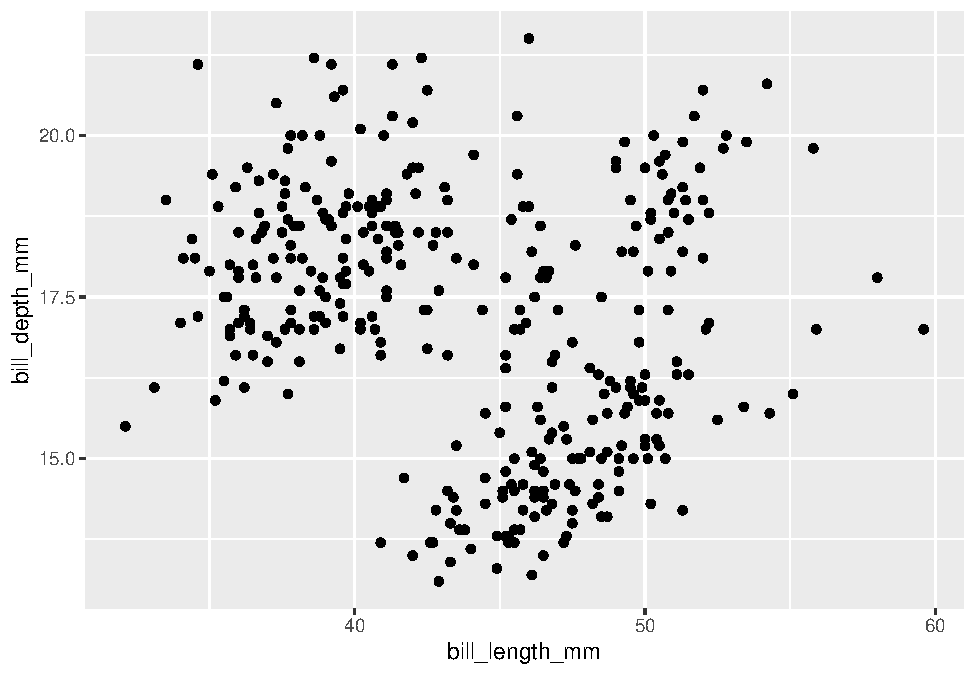
\includegraphics{_main_files/figure-latex/unnamed-chunk-52-1.pdf}

However, notice that the plot is empty. This is because we've only specified the first two layers of our graph: the data and the aesthetics. We haven't defined any geoms, or actual plotting methods, in our plot.

\subsection{Geoms}\label{geoms}

Geoms (short for geometries) define \emph{how} data is plotted. If \texttt{ggplot()} provides the basic canvas for the graph (i.e.~\emph{what} to plot), geoms are what create the graph (i.e.~\emph{how} it is plotted). Different graph types are defined using geoms. As per the diagram of the grammar of graphics above, we add (literally, using \texttt{+}) additional layers to our base \texttt{ggplot()} call in order to build our graph.

Refer to the cheatsheet for all of the possible geoms. For now, we will stick to some basics.

A scatter plot can be specified by adding \texttt{geom\_point()}. This requires that your x and y variables are continuous:

\begin{Shaded}
\begin{Highlighting}[]
\FunctionTok{ggplot}\NormalTok{(}\AttributeTok{data =}\NormalTok{ penguins, }\FunctionTok{aes}\NormalTok{(}\AttributeTok{x =}\NormalTok{ bill\_length\_mm, }\AttributeTok{y =}\NormalTok{ bill\_depth\_mm)) }\SpecialCharTok{+} 
  \FunctionTok{geom\_point}\NormalTok{()}
\end{Highlighting}
\end{Shaded}

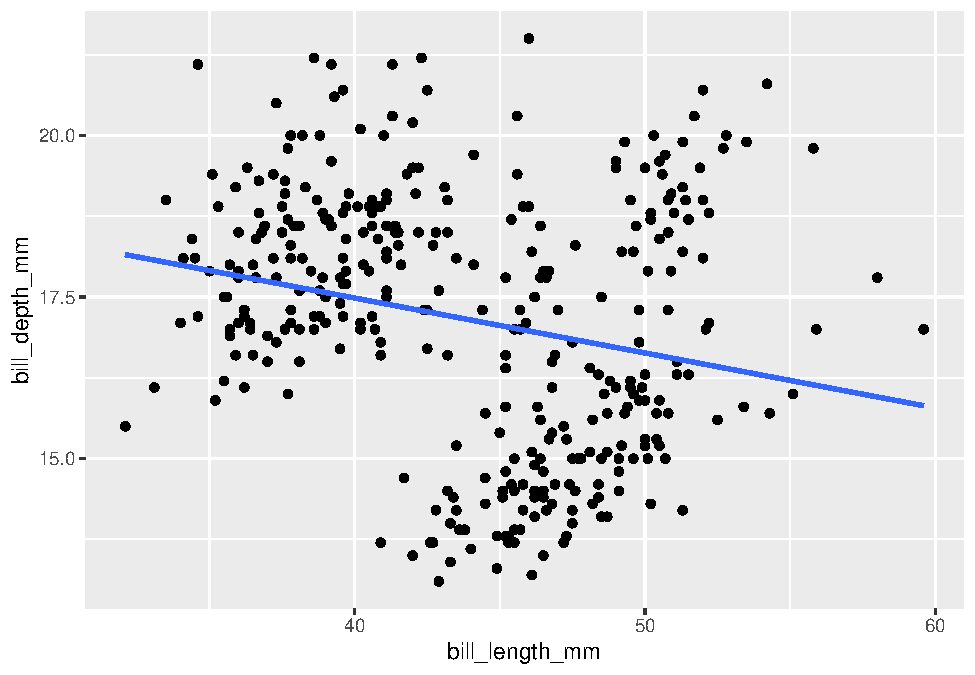
\includegraphics{_main_files/figure-latex/unnamed-chunk-53-1.pdf}

\texttt{geom\_smooth()} will add a line of best fit to a scatterplot. You can add this as another geom layer by adding \texttt{geom\_smooth(method\ =\ "lm")}. Specifying the method is important because by default, \texttt{geom\_smooth()} will probably fit LOESS curves (local polynomial regressions). Note that this function should be added after using \texttt{geom\_point()}.

By default, the line will also have standard error bands around it. You can turn this off by also specifying \texttt{se\ =\ FALSE} in the \texttt{geom\_smooth()} call.

\begin{Shaded}
\begin{Highlighting}[]
\FunctionTok{ggplot}\NormalTok{(}\AttributeTok{data =}\NormalTok{ penguins, }\FunctionTok{aes}\NormalTok{(}\AttributeTok{x =}\NormalTok{ bill\_length\_mm, }\AttributeTok{y =}\NormalTok{ bill\_depth\_mm)) }\SpecialCharTok{+} 
  \FunctionTok{geom\_point}\NormalTok{() }\SpecialCharTok{+}
  \FunctionTok{geom\_smooth}\NormalTok{(}\AttributeTok{method =} \StringTok{"lm"}\NormalTok{, }\AttributeTok{se =} \ConstantTok{FALSE}\NormalTok{)}
\end{Highlighting}
\end{Shaded}

\begin{verbatim}
## `geom_smooth()` using formula = 'y ~ x'
\end{verbatim}

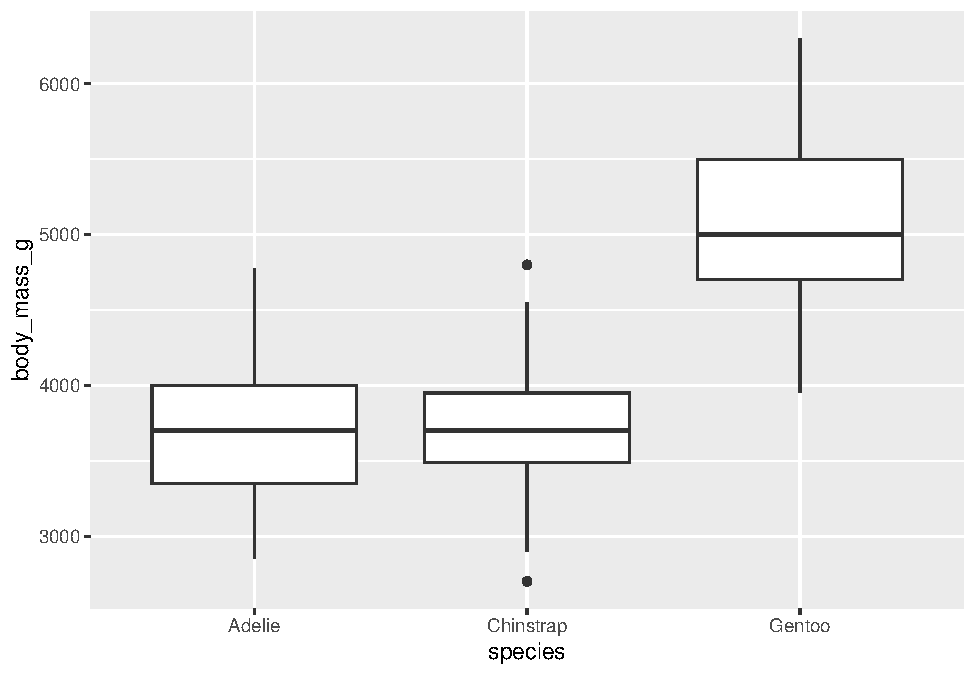
\includegraphics{_main_files/figure-latex/unnamed-chunk-54-1.pdf}

\texttt{geom\_boxplot()} will create boxplots. For this geom to work, a categorical variable must be on the x axis and a continuous variable must be on the y axis. An example is below, with species on the x axis and body mass on the y:

\begin{Shaded}
\begin{Highlighting}[]
\FunctionTok{ggplot}\NormalTok{(}\AttributeTok{data =}\NormalTok{ penguins, }\FunctionTok{aes}\NormalTok{(}\AttributeTok{x =}\NormalTok{ species, }\AttributeTok{y =}\NormalTok{ body\_mass\_g)) }\SpecialCharTok{+} 
  \FunctionTok{geom\_boxplot}\NormalTok{()}
\end{Highlighting}
\end{Shaded}

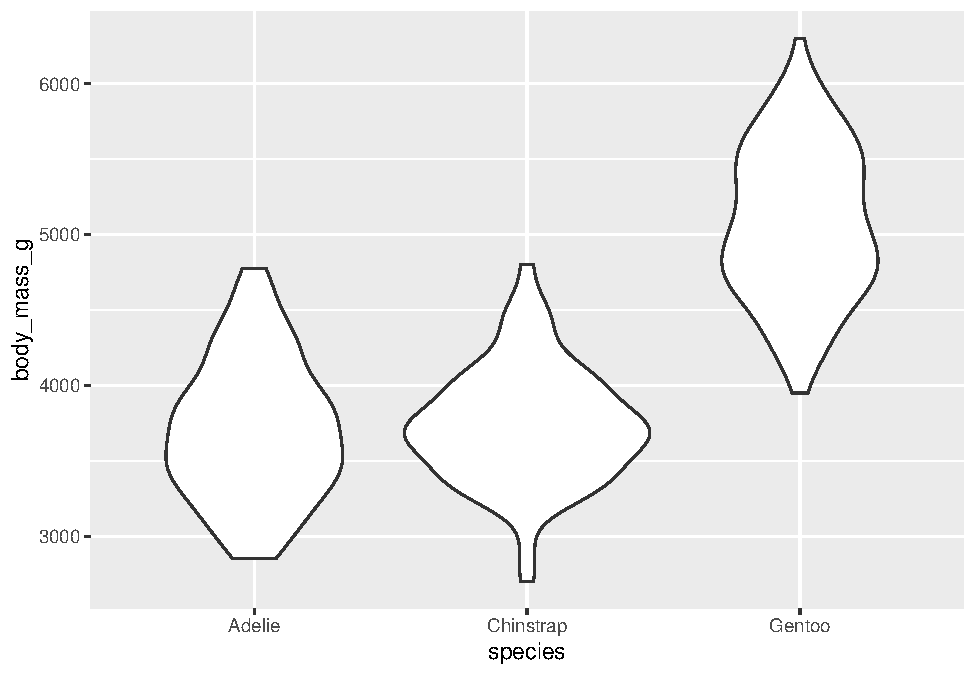
\includegraphics{_main_files/figure-latex/unnamed-chunk-55-1.pdf}

\texttt{geom\_violin()} plots violin plots, which is a variant of the boxplot that also plots the distribution.

\begin{Shaded}
\begin{Highlighting}[]
\FunctionTok{ggplot}\NormalTok{(}\AttributeTok{data =}\NormalTok{ penguins, }\FunctionTok{aes}\NormalTok{(}\AttributeTok{x =}\NormalTok{ species, }\AttributeTok{y =}\NormalTok{ body\_mass\_g)) }\SpecialCharTok{+} 
  \FunctionTok{geom\_violin}\NormalTok{()}
\end{Highlighting}
\end{Shaded}

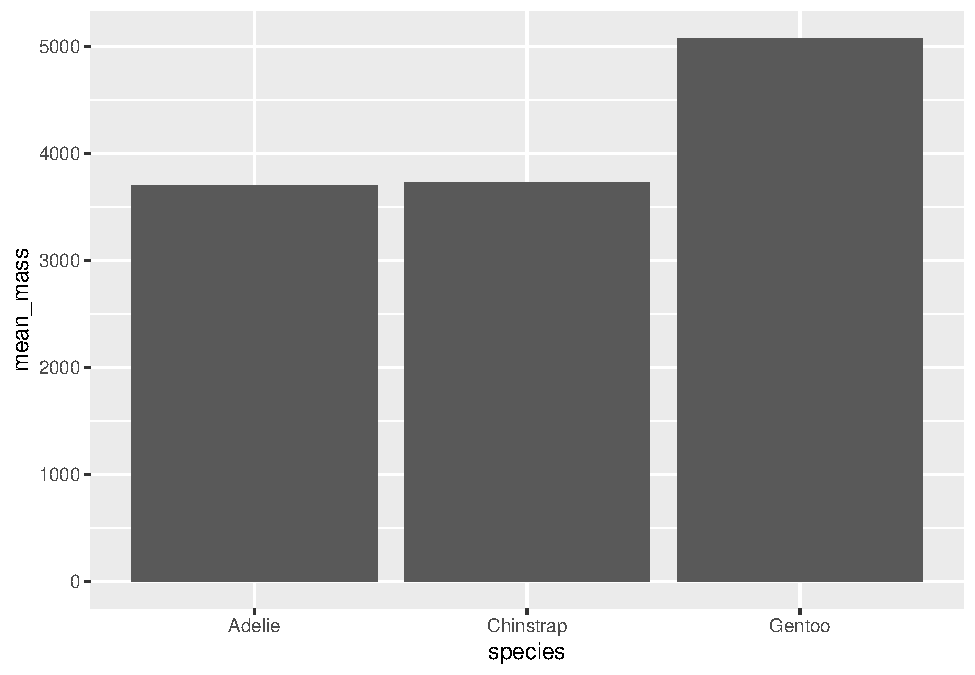
\includegraphics{_main_files/figure-latex/unnamed-chunk-56-1.pdf}

\texttt{geom\_bar()} and \texttt{geom\_col()} will both create bar plots, but their usage is slightly different. \texttt{geom\_bar()} is best used if you want to plot the \emph{number} of items in each category. \texttt{geom\_col()} is best used to plot means or similar statistics.

\begin{Shaded}
\begin{Highlighting}[]
\NormalTok{penguins }\SpecialCharTok{\%\textgreater{}\%}
  \FunctionTok{group\_by}\NormalTok{(species) }\SpecialCharTok{\%\textgreater{}\%}
  \FunctionTok{summarise}\NormalTok{(}
    \AttributeTok{mean\_mass =} \FunctionTok{mean}\NormalTok{(body\_mass\_g, }\AttributeTok{na.rm =} \ConstantTok{TRUE}\NormalTok{)}
\NormalTok{  ) }\SpecialCharTok{\%\textgreater{}\%}
  \FunctionTok{ggplot}\NormalTok{(}\FunctionTok{aes}\NormalTok{(}\AttributeTok{x =}\NormalTok{ species, }\AttributeTok{y =}\NormalTok{ mean\_mass)) }\SpecialCharTok{+}
  \FunctionTok{geom\_col}\NormalTok{()}
\end{Highlighting}
\end{Shaded}

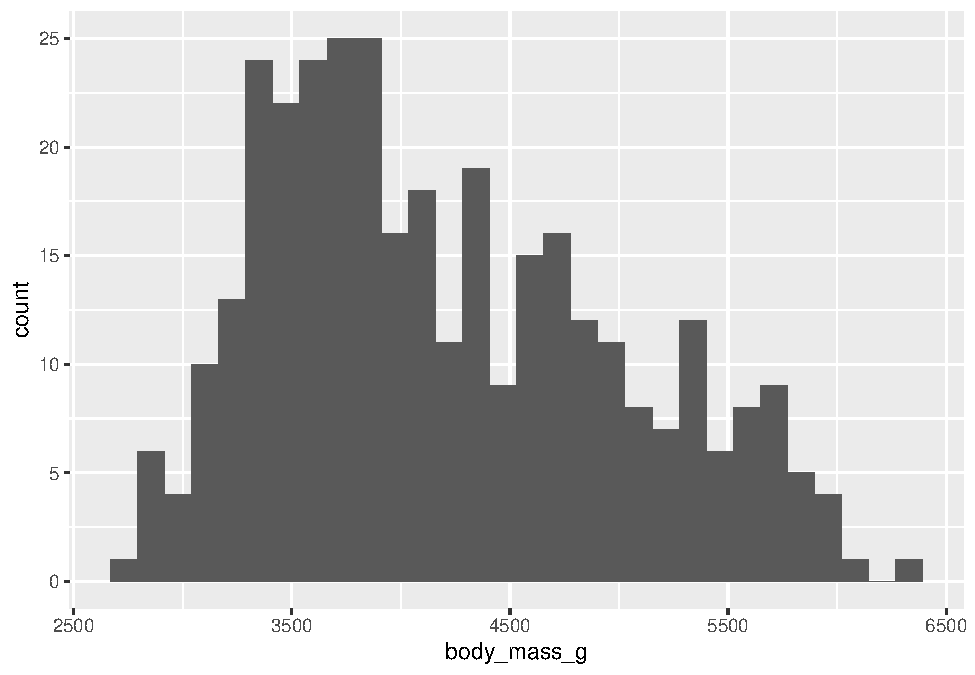
\includegraphics{_main_files/figure-latex/unnamed-chunk-57-1.pdf}

\texttt{geom\_histogram()} will plot a histogram, which is useful for visualising distributions. For this, you only need to provide one continuous variable on the x-axis. \texttt{geom\_density()} will plot the same information but using a smoothed line instead of bins.

\begin{Shaded}
\begin{Highlighting}[]
\FunctionTok{ggplot}\NormalTok{(}\AttributeTok{data =}\NormalTok{ penguins, }\FunctionTok{aes}\NormalTok{(}\AttributeTok{x =}\NormalTok{ body\_mass\_g)) }\SpecialCharTok{+} 
  \FunctionTok{geom\_histogram}\NormalTok{()}
\end{Highlighting}
\end{Shaded}

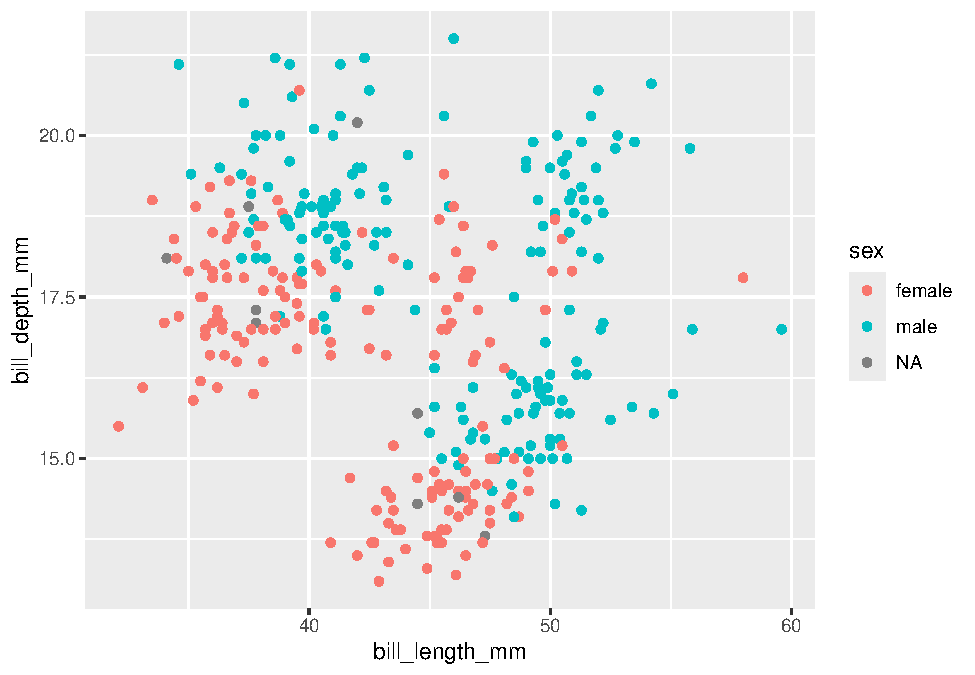
\includegraphics{_main_files/figure-latex/unnamed-chunk-58-1.pdf}

\begin{Shaded}
\begin{Highlighting}[]
\FunctionTok{ggplot}\NormalTok{(}\AttributeTok{data =}\NormalTok{ penguins, }\FunctionTok{aes}\NormalTok{(}\AttributeTok{x =}\NormalTok{ body\_mass\_g)) }\SpecialCharTok{+} 
  \FunctionTok{geom\_density}\NormalTok{()}
\end{Highlighting}
\end{Shaded}

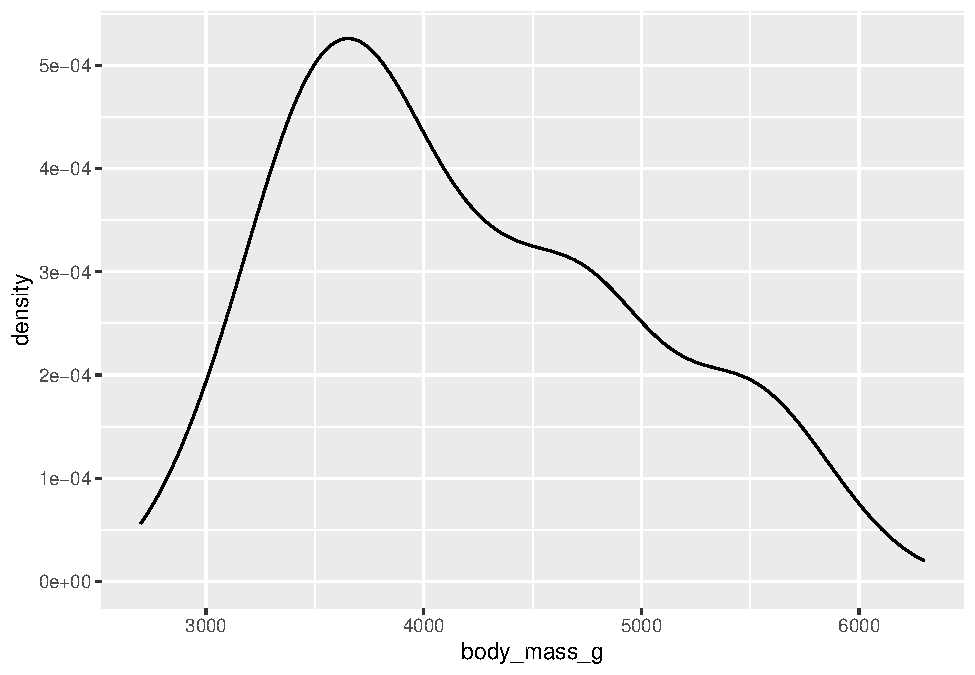
\includegraphics{_main_files/figure-latex/unnamed-chunk-58-2.pdf}

\subsection{Making the graph look better}\label{making-the-graph-look-better}

This is all well and good, and we already have workable basic graphs using \texttt{ggplot}. From here, we can change many things by adding or modifying our existing layers to our ggplot. There are \emph{so} many options available here, but here we'll only focus on some basic considerations.

An important aspect of data visualisation is a good use of colour. Colours should be used in both an informative and an aesthetically appealing way. A particularly common but effective use of colour is to use different colours to denote different groups in a plot.

\texttt{ggplot} provides two mechanisms within aesthetics for controlling colour. Both must typically be included in the \texttt{aes()} part of \texttt{ggplot()}.

\begin{itemize}
\tightlist
\item
  \texttt{colour} controls the colouring of points and lines. For graphs with shapes, such as boxplots and violin plots, this argument will control the colour of the border.
\item
  \texttt{fill} controls the colouring of anything over an area, such as bar plots, histograms and density/violin plots.
\end{itemize}

We can tell \texttt{gggplot} to colour in aspects of our graph based on another variable in the dataset we are using. For example, if we want to colour a scatterplot between two vraiables by sex (which is a column in the penguins data), we can do so by specifiyng \texttt{colour\ =\ sex} in our \texttt{aes()} function.

\begin{Shaded}
\begin{Highlighting}[]
\FunctionTok{ggplot}\NormalTok{(}\AttributeTok{data =}\NormalTok{ penguins, }\FunctionTok{aes}\NormalTok{(}\AttributeTok{x =}\NormalTok{ bill\_length\_mm, }\AttributeTok{y =}\NormalTok{ bill\_depth\_mm, }\AttributeTok{colour =}\NormalTok{ sex)) }\SpecialCharTok{+}
  \FunctionTok{geom\_point}\NormalTok{()}
\end{Highlighting}
\end{Shaded}

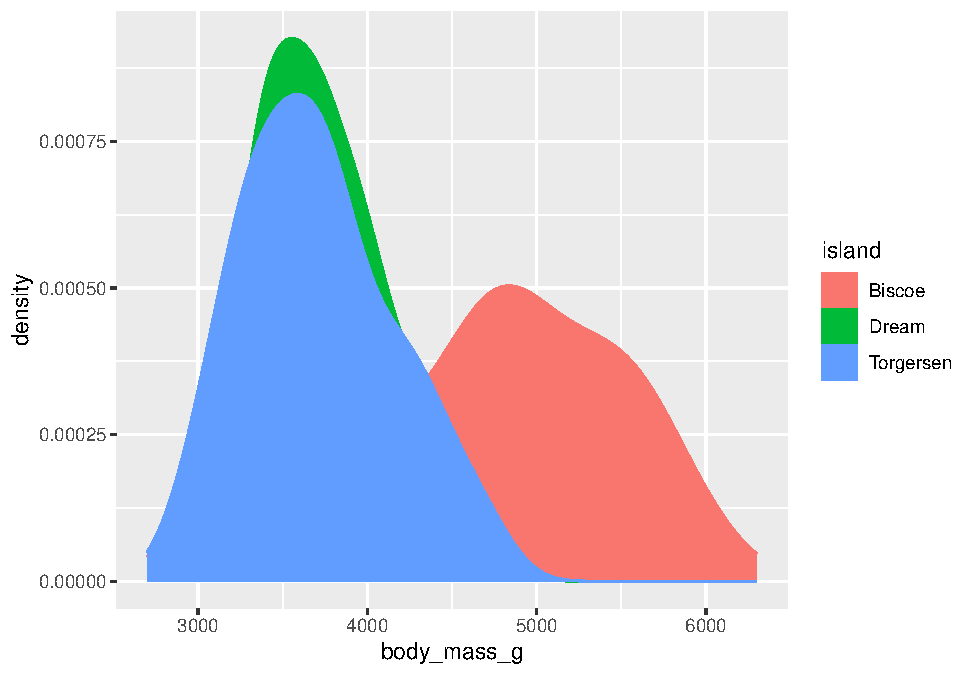
\includegraphics{_main_files/figure-latex/unnamed-chunk-59-1.pdf}

Many graphs allow for control of both colour and fill. In these instances, as noted above, \texttt{fill} controls the colour within the shape while \texttt{colour} controls the colour of the shape's edges. For example, here is a density plot that specifies both \texttt{colour} and \texttt{fill} to be controlled by the variable \texttt{island}. This has the effect of making both the borders and the area within the shape the same colour.

\begin{Shaded}
\begin{Highlighting}[]
\FunctionTok{ggplot}\NormalTok{(}\AttributeTok{data =}\NormalTok{ penguins, }\FunctionTok{aes}\NormalTok{(}\AttributeTok{x =}\NormalTok{ body\_mass\_g, }\AttributeTok{fill =}\NormalTok{ island, }\AttributeTok{colour =}\NormalTok{ island)) }\SpecialCharTok{+} 
  \FunctionTok{geom\_density}\NormalTok{()}
\end{Highlighting}
\end{Shaded}

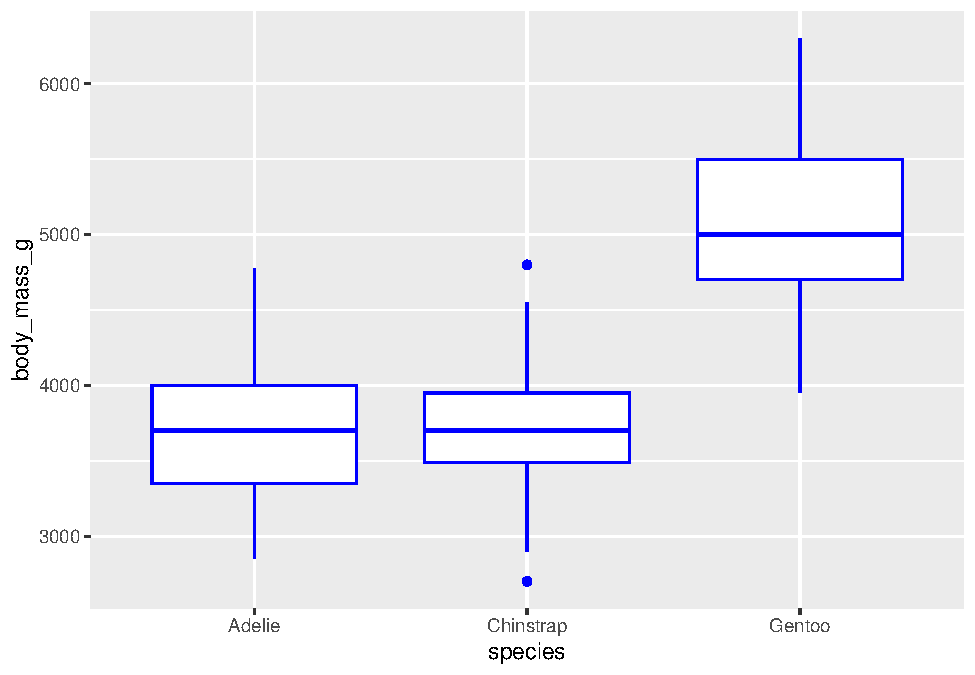
\includegraphics{_main_files/figure-latex/unnamed-chunk-60-1.pdf}

Now, this is all well and good but in this particular instance the overlapping of curves means that we can't actually see what is going on very well. The data points from Torgersen island, for instance, almost completely overlap with the data points from Dream Island. One way to get past this is to specify another aesthetic called \texttt{alpha}, which sets the \textbf{transparency} of the fill.

As we typically only want to change the transparency of one type of geom in a plot, the best place to include an \texttt{alpha} argument is within the geom call itself (in this case, within \texttt{geom\_density()}). \texttt{alpha} can range from 0 - 1, where 1 means an object is 100\% opaque (i.e.~0\% transparent) and 0 means 0\% opaqueness (100\% transparency). Here, we use \texttt{alpha\ =\ 0.5} to set the fill to be 50\% transparent:

\begin{Shaded}
\begin{Highlighting}[]
\FunctionTok{ggplot}\NormalTok{(}\AttributeTok{data =}\NormalTok{ penguins, }\FunctionTok{aes}\NormalTok{(}\AttributeTok{x =}\NormalTok{ body\_mass\_g, }\AttributeTok{fill =}\NormalTok{ island, }\AttributeTok{colour =}\NormalTok{ island)) }\SpecialCharTok{+} 
  \FunctionTok{geom\_density}\NormalTok{(}\AttributeTok{alpha =} \FloatTok{0.5}\NormalTok{)}
\end{Highlighting}
\end{Shaded}

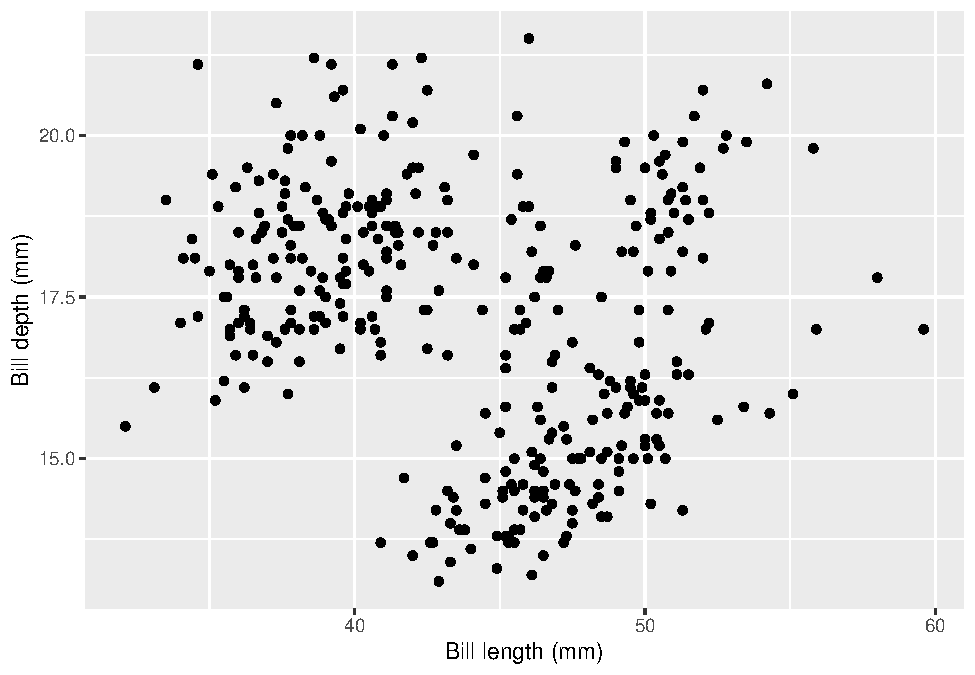
\includegraphics{_main_files/figure-latex/unnamed-chunk-61-1.pdf}
Now we can see the outlines of each density curve more clearly! This is great.

\texttt{ggplot} also supports the manual specification of colours. R by default comes with a bunch of strings that are recognised as colours during graphing, such as \texttt{"black"}, \texttt{"blue"} and \texttt{"red"}. These can be used to manually set either the colour or the fill of a geom. To use these, you can instead use \texttt{colour}/\texttt{fill} within the \emph{geom} like so:

\begin{Shaded}
\begin{Highlighting}[]
\FunctionTok{ggplot}\NormalTok{(}\AttributeTok{data =}\NormalTok{ penguins, }\FunctionTok{aes}\NormalTok{(}\AttributeTok{x =}\NormalTok{ species, }\AttributeTok{y =}\NormalTok{ body\_mass\_g)) }\SpecialCharTok{+} 
  \FunctionTok{geom\_boxplot}\NormalTok{(}\AttributeTok{colour =} \StringTok{"blue"}\NormalTok{)}
\end{Highlighting}
\end{Shaded}

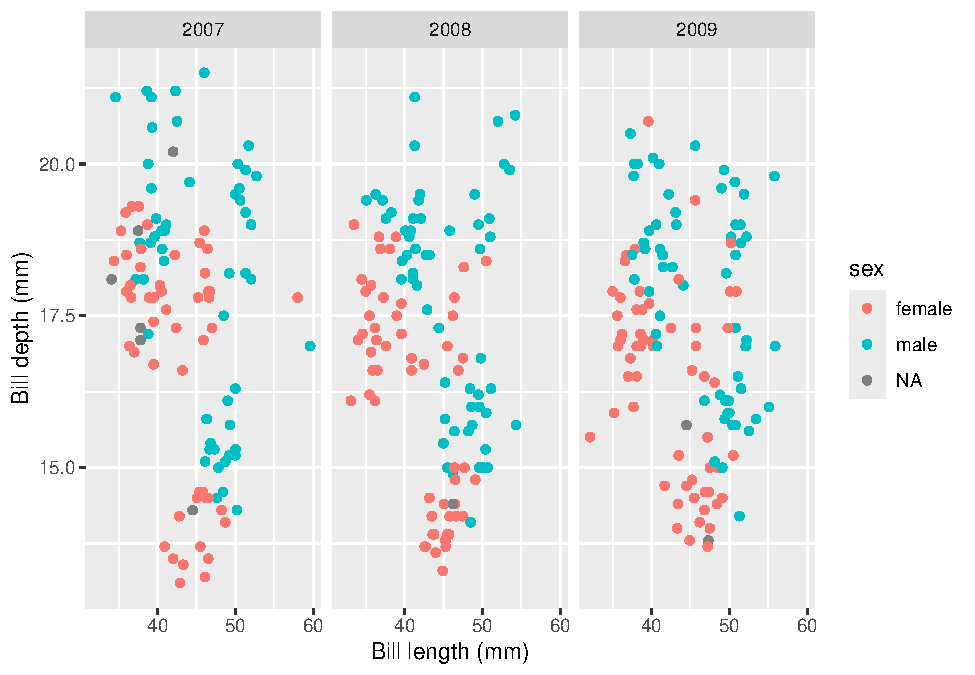
\includegraphics{_main_files/figure-latex/unnamed-chunk-62-1.pdf}

You can also provide hexadecimal strings (e.g.~``white'' corresponds to \texttt{"\#FFFFFF"}). See \hyperref[colours]{the Appendix} for a full list of the basic palettes in R.

Every graph needs good axis titles. By default, \texttt{ggplot} will use variable names as axis labels, which often aren't very informative by default. We can change this by adding \texttt{labs()}, which is a simple way of specifying x and y labels:

\begin{Shaded}
\begin{Highlighting}[]
\FunctionTok{ggplot}\NormalTok{(}\AttributeTok{data =}\NormalTok{ penguins, }\FunctionTok{aes}\NormalTok{(}\AttributeTok{x =}\NormalTok{ bill\_length\_mm, }\AttributeTok{y =}\NormalTok{ bill\_depth\_mm)) }\SpecialCharTok{+} 
  \FunctionTok{geom\_point}\NormalTok{() }\SpecialCharTok{+}
  \FunctionTok{labs}\NormalTok{(}\AttributeTok{x =} \StringTok{"Bill length (mm)"}\NormalTok{, }\AttributeTok{y =} \StringTok{"Bill depth (mm)"}\NormalTok{) }
\end{Highlighting}
\end{Shaded}

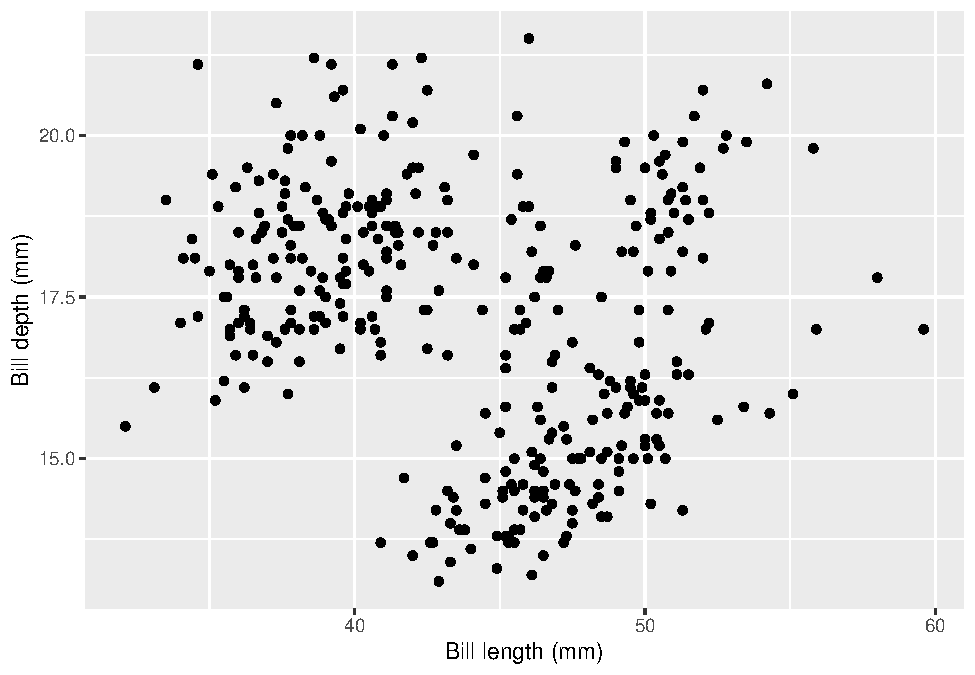
\includegraphics{_main_files/figure-latex/unnamed-chunk-63-1.pdf}

Finally, if you want to split plots by a certain variable, add \texttt{facet\_wrap()} to your call. You need to specify what variable/column you want to split by, with a tilde in front. For example, if we wanted to split the scatter plot by year:

\begin{Shaded}
\begin{Highlighting}[]
\FunctionTok{ggplot}\NormalTok{(}\AttributeTok{data =}\NormalTok{ penguins, }\FunctionTok{aes}\NormalTok{(}\AttributeTok{x =}\NormalTok{ bill\_length\_mm, }\AttributeTok{y =}\NormalTok{ bill\_depth\_mm, }\AttributeTok{colour =}\NormalTok{ sex)) }\SpecialCharTok{+} \FunctionTok{geom\_point}\NormalTok{() }\SpecialCharTok{+}
  \FunctionTok{labs}\NormalTok{(}\AttributeTok{x =} \StringTok{"Bill length (mm)"}\NormalTok{, }\AttributeTok{y =} \StringTok{"Bill depth (mm)"}\NormalTok{)  }\SpecialCharTok{+} 
  \FunctionTok{facet\_wrap}\NormalTok{(}\SpecialCharTok{\textasciitilde{}}\NormalTok{year)}
\end{Highlighting}
\end{Shaded}

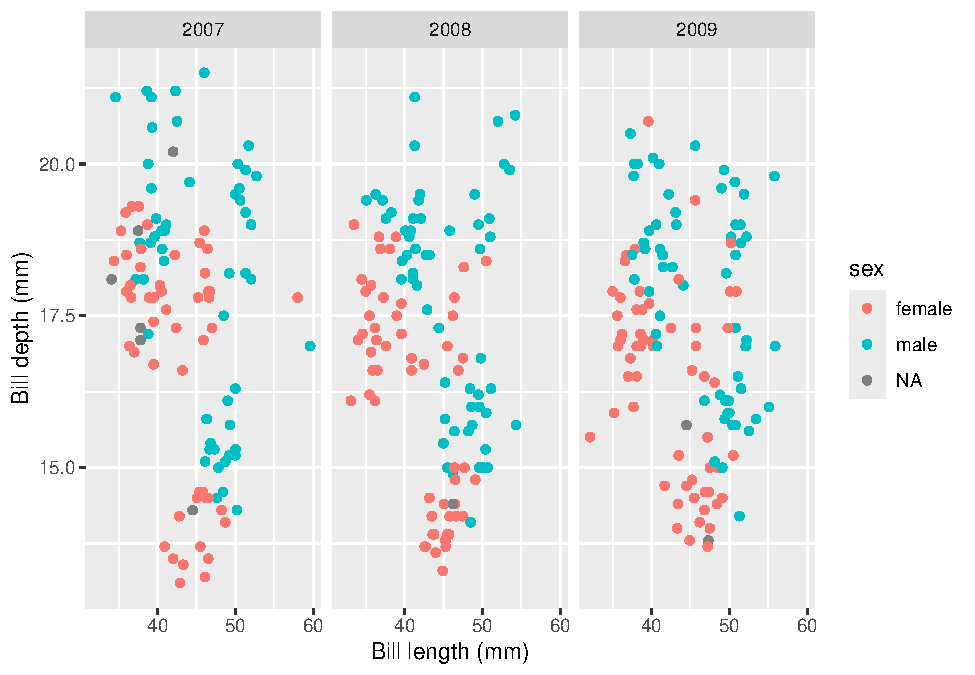
\includegraphics{_main_files/figure-latex/unnamed-chunk-64-1.pdf}

You can see that the graph now creates one graph per year, which can be immensely useful for visualising data points between groups.

From here, there are so many things you can do with ggplot - and it helps to get creative!

\chapter{Descriptive statistics (Module 5)}\label{descriptives}

Descriptive statistics, as the name implies, are used to describe data. A key part of the quantitative research process is understanding the various ins and outs of your data. You'll probably have a sense of why this is important if you have the qualitative presentation still fresh in your mind - namely, knowing your data is also really important for knowing what to do with it.

In this first module, we will start with the first steps of understanding quantitative data. This involves visualising our data to see what it looks like, and describing key features of the data. If you're familiar with statistics then some of this may seem a bit trivial, but it's important that we get the basics right before we go on to doing fancy statistical tests.

\begin{quote}
Also, I know that the idea of doing statistics and maths freaks a lot of us out - and that's totally normal. Yes, there will be some number-crunching and maths in the next series of modules, but the focus of these modules is not to force you to calculate things by hand. You will encounter a whole bunch of mathematical formulae, but the point of doing so is to illustrate the concepts that underpin them. These concepts are crucial to understanding the `magic' that happens with quantitative analysis, and a really solid foundation in statistical concepts will go a long way.
\end{quote}

\begin{quote}
That being said, throughout these statistics modules there will be a number of activities that ask you to actively work with sample datasets and analyse them. We promise that you will get so much more out of these modules if you complete these activities, because readings and webpages aren't the best substitute for actually doing it and getting your hands dirty with data.
\end{quote}

By the end of this module you should be able to:

\begin{itemize}
\tightlist
\item
  Create both appropriate and meaningful graphs from data
\item
  Calculate various forms of descriptive statistics
\item
  Interpret both graphs and descriptive statistics, and explain what they tell you
\end{itemize}

\section{Visualising data}\label{visualising-data}

When you have data in your hand, it is often tempting to dive straight into plugging it into an analysis and seeing what the results are. However, in general this is unwise. The first step in working with quantitative data is to see what your data looks like. Looking at the data can give us a first glance into many aspects of the results, which can be informative for analyses.

\subsection{Why visualise data?}\label{why-visualise-data}

\begin{quote}
``The greatest value of a picture is when it forces us to notice what we never expected to see.'' -John W. Tukey
\end{quote}

One of the first steps in working with quantitative data is data visualisation, which is the process of graphing it and looking at it. If you work with quantitative data then it should become standard practice for you to graph your data before analysing it.

It's common for many students learning research methods and statistics to simply take a `cookie cutter' approach - that is, collect data, run basic tests on it and call it a day. Sadly this is common even at our level, and you will almost certainly see this happen at music psychology conferences that you go to in future. People will present complex analyses that sound impressive - until you pick up on small cues that suggest they don't really understand their data at all.

Below is an example of why data visualisation should be a crucial part of the quantitative research process:

\includegraphics{img/datasaurus.gif}

This series of datasets is called the \href{https://www.research.autodesk.com/publications/same-stats-different-graphs/}{Datasaurus Dozen}, which are 12 datasets that look entirely different (including the dinosaur!) but share almost identical summary statistics, as shown by the bold numbers on the right.

Data visualisation is important because:

\begin{enumerate}
\def\labelenumi{\arabic{enumi}.}
\tightlist
\item
  It lets you observe patterns in your data.
\item
  It can reveal unexpected structures in your data that would normally be missed otherwise.
\item
  It is an effective way of communicating information. The best graphs tell a reader everything they need to know in one image.
\end{enumerate}

In the Canvas version of this subject, there are some general guidelines as to how to make good figures right around this point. For this version of the book, the \hyperref[ggplot]{section on ggplot} is going to be infinitely better.

Regardless of which graph you use, every good graph should have the basic following features:

Content made with H5P.

\section{Counts and central tendencies}\label{basic-desc}

Once we understand what our data looks like, we can then move to describing the general properties of the data. Such general properties are called descriptive statistics. Reporting descriptive statistics is crucial for many aspects of quantitative research.

\subsection{Basic features}\label{count-basics}

There are a couple of basic features of any dataset that should be looked at and noted:

\begin{tabular}{l|l|l}
\hline
Name (APA Symbol) & Definition & When to report?\\
\hline
Count (n) & The number of data points. & The number of participants should always be reported - not just for the sample as a whole, but for each analysis done.\\
\hline
Range & In the context of writing up statistics, this is usually the minimum and maximum values. & Reporting these values is often useful as a range when writing up demographic variables, e.g. age or years of training.\\
\hline
Percentages &  & Use primarily for categorical data, e.g. sex or groups.\\
\hline
\end{tabular}

We can use R to find some of these values, either using straight base R or tidyverse functions. For this page/module only, I will use the \texttt{variable\_a} mock variable from \hyperref[vectors]{Section 2.2.2} with a minor amendment:

\begin{Shaded}
\begin{Highlighting}[]
\NormalTok{vector\_a }\OtherTok{\textless{}{-}} \FunctionTok{c}\NormalTok{(}\DecValTok{4}\NormalTok{, }\DecValTok{1}\NormalTok{, }\DecValTok{6}\NormalTok{, }\DecValTok{2}\NormalTok{, }\DecValTok{3}\NormalTok{, }\DecValTok{4}\NormalTok{)}
\NormalTok{vector\_a}
\end{Highlighting}
\end{Shaded}

\begin{verbatim}
## [1] 4 1 6 2 3 4
\end{verbatim}

For tidyverse usage, I'll refer to \texttt{df\_a}, which is just the same but as a one-column dataframe:

\begin{Shaded}
\begin{Highlighting}[]
\NormalTok{df\_a}
\end{Highlighting}
\end{Shaded}

\begin{verbatim}
##   column_a
## 1        4
## 2        1
## 3        6
## 4        2
## 5        3
## 6        4
\end{verbatim}

To find the \emph{count}, or the number of items in a vector, we can use the \texttt{length()} function.

\begin{Shaded}
\begin{Highlighting}[]
\FunctionTok{length}\NormalTok{(vector\_a)}
\end{Highlighting}
\end{Shaded}

\begin{verbatim}
## [1] 6
\end{verbatim}

To find the minimum and maximum, we can use the \texttt{min()} and \texttt{max()} functions respectively. Specifying \texttt{na.rm\ =\ TRUE} will remove any missing data before calculation.

\begin{Shaded}
\begin{Highlighting}[]
\FunctionTok{min}\NormalTok{(vector\_a, }\AttributeTok{na.rm =} \ConstantTok{TRUE}\NormalTok{)}
\end{Highlighting}
\end{Shaded}

\begin{verbatim}
## [1] 1
\end{verbatim}

\begin{Shaded}
\begin{Highlighting}[]
\FunctionTok{max}\NormalTok{(vector\_a, }\AttributeTok{na.rm =} \ConstantTok{TRUE}\NormalTok{)}
\end{Highlighting}
\end{Shaded}

\begin{verbatim}
## [1] 6
\end{verbatim}

In tidyverse fashion, we can wrap this all in \texttt{summarise()} as follows:

\begin{Shaded}
\begin{Highlighting}[]
\NormalTok{df\_a }\SpecialCharTok{\%\textgreater{}\%}
  \FunctionTok{summarise}\NormalTok{(}
    \AttributeTok{n =} \FunctionTok{n}\NormalTok{(),}
    \AttributeTok{min =} \FunctionTok{min}\NormalTok{(column\_a, }\AttributeTok{na.rm =} \ConstantTok{TRUE}\NormalTok{),}
    \AttributeTok{max =} \FunctionTok{max}\NormalTok{(column\_a, }\AttributeTok{na.rm =} \ConstantTok{TRUE}\NormalTok{)}
\NormalTok{  )}
\end{Highlighting}
\end{Shaded}

\begin{verbatim}
##   n min max
## 1 6   1   6
\end{verbatim}

\subsection{Central tendencies}\label{central-tendency}

While the range can be informative in some sitautions, it usually isn't enough to draw deeper interpretations from raw data. One key way of describing data is in terms of central tendency - or where the `average' value approximately is. There are three main types of central tendency, summarized in the table below.

\begin{tabular}{l|l|l|l}
\hline
Name (APA Symbol) & Definition & When to use? & Things to note\\
\hline
Mean (M) & The sum of all values, divided by the number of data points. & Use if data is normally distributed. & Can be influenced by outliers, so generally unsuitable when data is skewed.\\
\hline
Median (Mdn) & The 'middle' data point, when sorted in order. & Use for skewed data, or for ordinal data. & Generally is less preferable to the mean, except for use in skewed/ordinal data.\\
\hline
Mode & The most frequent value. & Use for nominal data. & Unsuitable for most other types of data.\\
\hline
\end{tabular}

To calculate a mean and median, use the \texttt{mean()} and \texttt{median()} functions respectively. Both functions also take the \texttt{na.rm} argument.

\begin{Shaded}
\begin{Highlighting}[]
\FunctionTok{mean}\NormalTok{(vector\_a, }\AttributeTok{na.rm =} \ConstantTok{TRUE}\NormalTok{)}
\end{Highlighting}
\end{Shaded}

\begin{verbatim}
## [1] 3.333333
\end{verbatim}

\begin{Shaded}
\begin{Highlighting}[]
\FunctionTok{median}\NormalTok{(vector\_a, }\AttributeTok{na.rm =} \ConstantTok{TRUE}\NormalTok{)}
\end{Highlighting}
\end{Shaded}

\begin{verbatim}
## [1] 3.5
\end{verbatim}

\begin{Shaded}
\begin{Highlighting}[]
\CommentTok{\# Using summarise() and piping}

\NormalTok{df\_a }\SpecialCharTok{\%\textgreater{}\%}
  \FunctionTok{summarise}\NormalTok{(}
    \AttributeTok{mean =} \FunctionTok{mean}\NormalTok{(column\_a, }\AttributeTok{na.rm =} \ConstantTok{TRUE}\NormalTok{),}
    \AttributeTok{median =} \FunctionTok{median}\NormalTok{(column\_a, }\AttributeTok{na.rm =} \ConstantTok{TRUE}\NormalTok{)}
\NormalTok{  )}
\end{Highlighting}
\end{Shaded}

\begin{verbatim}
##       mean median
## 1 3.333333    3.5
\end{verbatim}

Interestingly, R doesn't offer a base function to calculate a mode - if you need this information, you either need to manually work this out or turn to a package that offers it. One such example is the fantastic \texttt{DescTools} package, which provides a function called \texttt{Mode()}:

\begin{Shaded}
\begin{Highlighting}[]
\NormalTok{DescTools}\SpecialCharTok{::}\FunctionTok{Mode}\NormalTok{(vector\_a)}
\end{Highlighting}
\end{Shaded}

\begin{verbatim}
## [1] 4
## attr(,"freq")
## [1] 2
\end{verbatim}

The first number is the value of the mode, while the second number is the number of times the mode occurs (twice, in this case).

\section{Variability}\label{variability}

The other important part of describing data is in how spread out it is. Is our data tightly bunched together, or is it very spread out? This helps us understand where most of our data falls, as well as how it looks.

\subsection{The variability of data}\label{the-variability-of-data}

The other key way of describing data is in its spread, or distribution. The way data is distributed can give key insights into how that data should be treated.

Consider the following graphs below.

\begin{center}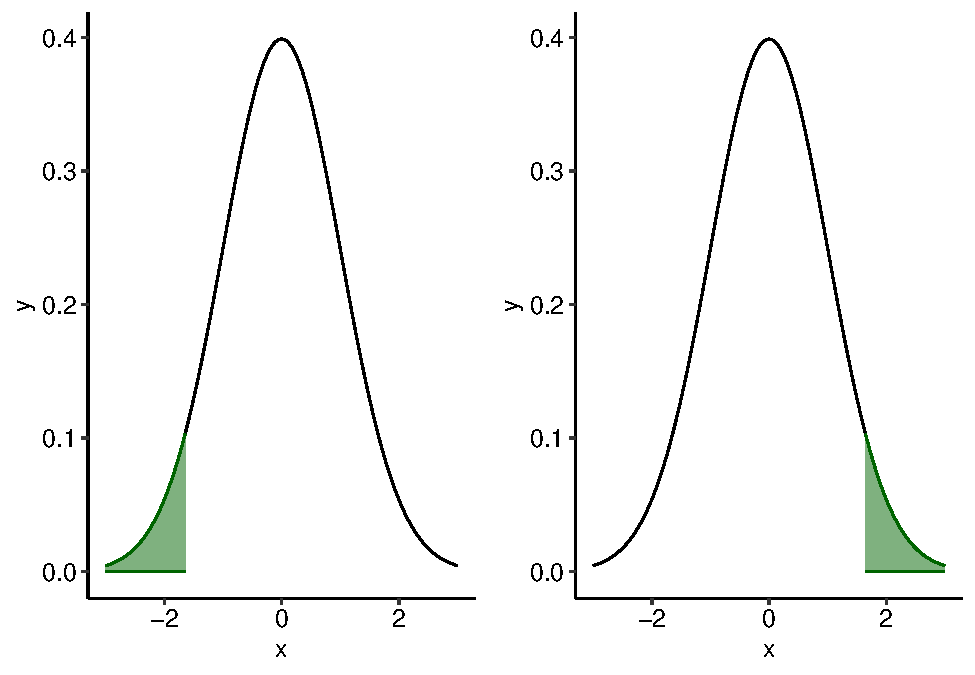
\includegraphics{_main_files/figure-latex/unnamed-chunk-78-1} \end{center}

You can see that all three graphs peak at around the same point, but \emph{look} very different outside of that. The orange line is narrow, while the red line is considerably more spread out. All of these graphs peak at the same point but still look very different. Therefore, they have very different \textbf{spreads}, or \textbf{distributions}.

We saw on the last page that we can quantify how far values are spread apart by finding the range. However, this isn't always a good idea - two datasets with the exact same range can look wildly different. Therefore, we need ways of quantifying how data is spread out as well.

\subsection{Standard deviation}\label{sd}

\textbf{Standard deviation} (\(\sigma\) or \textbf{SD}) describes how spread out our data is within our sample, in standard (i.e.~comparable) units. Data that is spread out widely (like the red curve above) will have a large standard deviation; likewise, data that has a narrow spread will have a small standard deviation. We'll touch on this a bit more in the following pages, but for now just remember what a standard deviation is for.

To calculate standard deviation, we first calculate \textbf{variance}, which is another measure of spread:

\[
 Variance = \frac{\Sigma (x_i - \bar{x} )^2}{n - 1}
\]

Or, in human terms:

\begin{itemize}
\tightlist
\item
  Take each data point (xi)
\item
  Subtract the mean from each data point (x with the bar) and square that difference
\item
  Add them all up together
\item
  Divide by n - 1
\end{itemize}

And then to calculate standard deviation, we simply take the square root of the variance.

\[
SD = \sqrt{Variance}
\]
Or, in full formula form:

\[
SD = \sqrt{\frac{\Sigma (x_i - \bar{x} )^2}{n - 1}}
\]

Standard deviations (SD) should reported alongside means when results are written up (consult an APA guide).

To calculate standard deviations in R, use the \texttt{sd()} function. Once again, this has an \texttt{na.rm} argument you can specify.

\begin{Shaded}
\begin{Highlighting}[]
\FunctionTok{sd}\NormalTok{(vector\_a, }\AttributeTok{na.rm =} \ConstantTok{TRUE}\NormalTok{)}
\end{Highlighting}
\end{Shaded}

\begin{verbatim}
## [1] 1.75119
\end{verbatim}

\begin{Shaded}
\begin{Highlighting}[]
\CommentTok{\# Tidyverse form}
\NormalTok{df\_a }\SpecialCharTok{\%\textgreater{}\%}
  \FunctionTok{summarise}\NormalTok{(}
    \AttributeTok{sd =} \FunctionTok{sd}\NormalTok{(column\_a, }\AttributeTok{na.rm =} \ConstantTok{TRUE}\NormalTok{)}
\NormalTok{  )}
\end{Highlighting}
\end{Shaded}

\begin{verbatim}
##        sd
## 1 1.75119
\end{verbatim}

\subsection{Standard error, and the SDoTM}\label{sderr}

Imagine that I have a population of 100 regular people (shown on the left). I take a sample of 10 people, measure their heights and then calculate the mean height of that one sample. I then repeat this process over and over again, and plot where each sample's mean falls. Of course, because every sample is slightly different the mean of each sample will be slightly different too due to sampling error. Some sample means will be lower than the true population mean, while some will be higher. Eventually, we might end up with something like this:

The spread of these sample means is called the sampling distribution of the mean (SDoTM), shown on the right. This gives us a sense of where the population mean (the parameter that we are interested in) might lie. With enough samples, the peak of this sampling distribution of the mean will converge around the population mean. As you can see in our hypothetical example, the peak of the sampling distribution of the mean sits pretty close to the original population mean, meaning our estimate is pretty good.

The standard error of the mean (standard error; SE) is another measure of variability - this time, it is the spread of sample means across the sampling distribution of the mean. This represents how close our sample mean is to the likely population mean. If our sampling distribution is wide, our standard error will be large - and that means that we won't have a very precise estimate of the population mean. However, if we have a small standard error that will mean that our sample mean is likely to be close to the population mean.

Standard error is calculated using the below formula:

\[
SE = \frac{SD}{\sqrt n}
\]

Where SD = standard deviation, and n = sample size.

Practice: You have a dataset of 400 people. You know that the mean of the DV is 760, with a standard deviation of 40. Calculate the standard error for this sample.

\section{Distributions}\label{distributions}

The `shape' of our data is equally important. What does our data actually look like? Does it even matter what it looks like? The topic of distributions in statistics and probability can make up its own subject (in fact it does), but here we discuss the basics below.

\subsection{The normal distribution}\label{normal-dist}

Earlier, we saw a series of graphs overlaid on top of each other. These graphs, while having different variability, were essentially all the same shape - they were symmetrical bell curves. These were all examples of the normal distribution (also called the Gaussian distribution). The classic normal distribution takes on a neat bell-shaped curve:

\begin{center}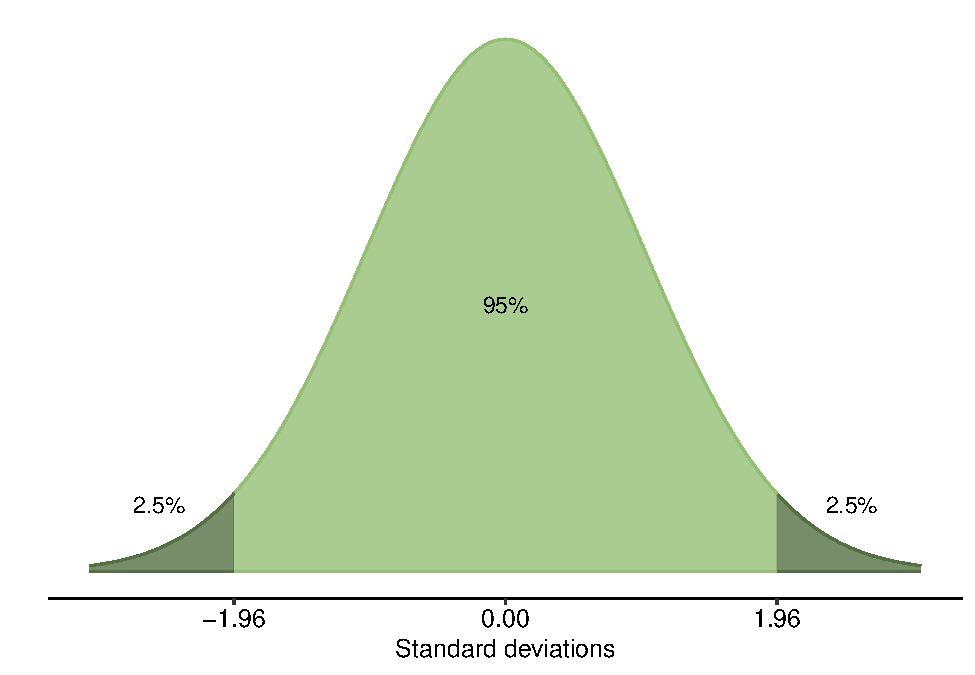
\includegraphics{_main_files/figure-latex/unnamed-chunk-80-1} \end{center}

In the normal distribution, the majority of data points cluster in the middle, while all other values are symmetrically distributed from either side from the middle. This is what gives the normal distribution its recognisable bell shape.

The normal distribution is defined by two parameters: the mean and the standard deviation of the data. These two parameters define the overall shape of the bell curve - the mean defines where the peak is, while the standard deviation defines how spread out the tails are.

An important feature of the normal distribution is where all of the data is spread, regardless of its shape: 95\% of the data within the curve falls within 1.96 standard deviations, either side of the mean. This applies to any normal distribution no matter what the scale of the data is. 99.7\% of data falls within just below 3 standard deviations.

\begin{center}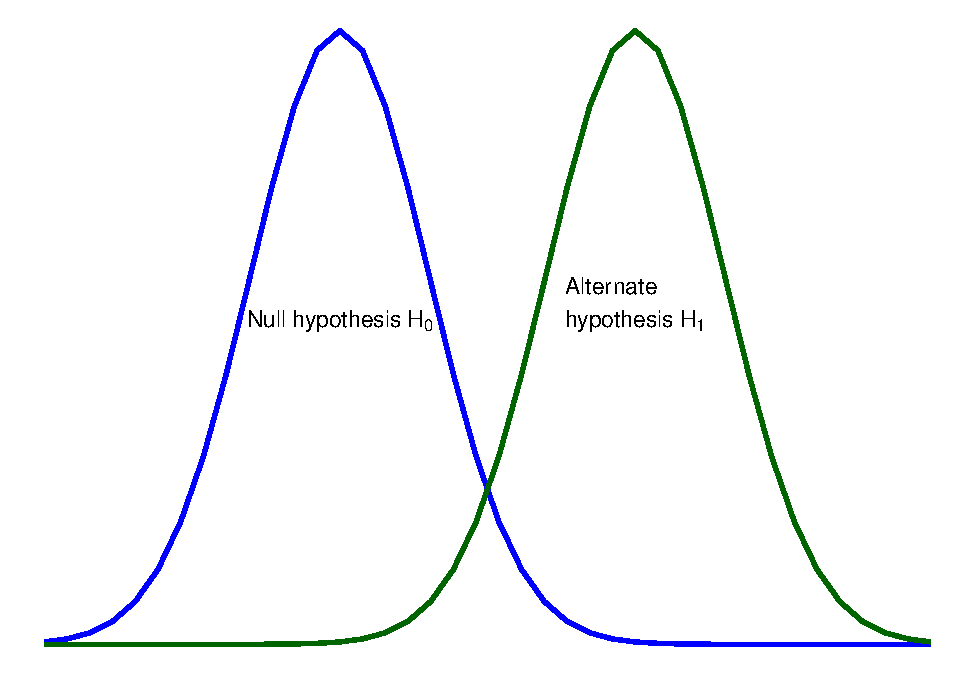
\includegraphics{_main_files/figure-latex/unnamed-chunk-81-1} \end{center}

\subsection{Skew}\label{skew}

Skewness, as the name implies, describes whether or not a distribution is symmetrical or skewed. If a distribution is skewed, we would expect numbers to be bunched up at one end of the distribution. Have a look at the three graphs below:

\begin{center}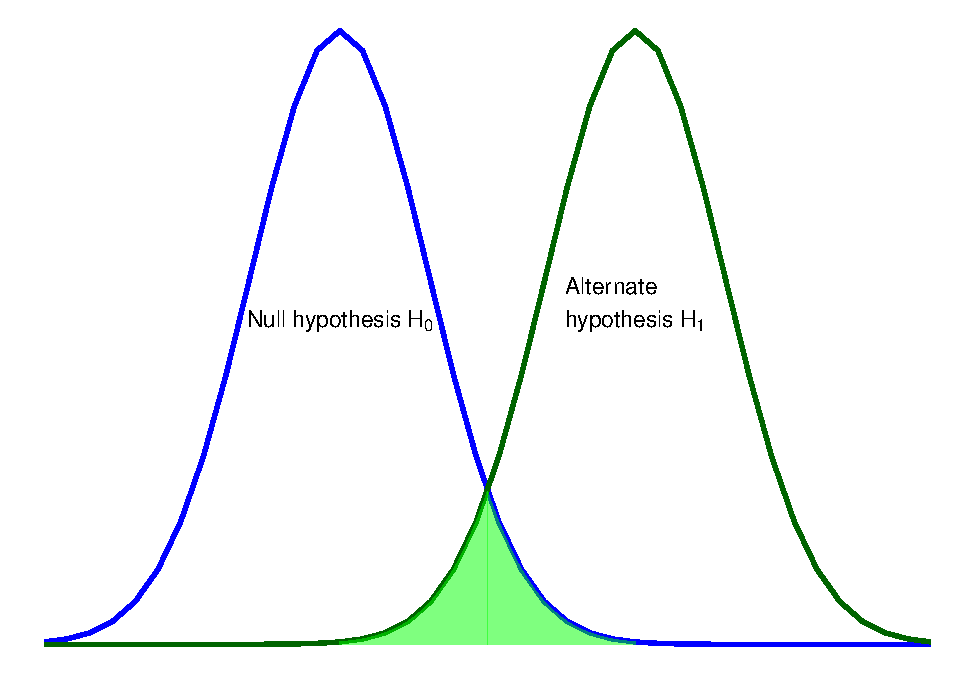
\includegraphics{_main_files/figure-latex/unnamed-chunk-82-1} \end{center}

\begin{itemize}
\tightlist
\item
  The purple graph in the middle is symmetrically distributed, so we say that it has no skew.
\item
  The red graph has values that are weighted towards the right-hand side of the x-axis, and so we say that it is either skewed left or negatively skewed.
\item
  The blue graph, on the other hand is skewed right or positively skewed. The left-right refers to which end the tail of the distribution is on.
\end{itemize}

Skewness can also be quantified numerically:

\begin{itemize}
\tightlist
\item
  A skewness of 0 means that a distribution is normal
\item
  A positive skew value means that the data is skewed right
\item
  A negative skew value means that the data is skewed left
\end{itemize}

As a general rule, if a distribution has a skew greater than +1 or lower than -1, it is skewed. If your data is skewed then this is a bit of an issue; there's a nice overview of this point and one way of dealing with skew in this blog post.

\subsection{Kurtosis}\label{kurtosis}

Kurtosis refers to the shape of the tails specifically. Are all of the data bunched very tightly around one value, or are the data evenly spread out? The three graphs you saw up above all have different kurtoses.

\begin{center}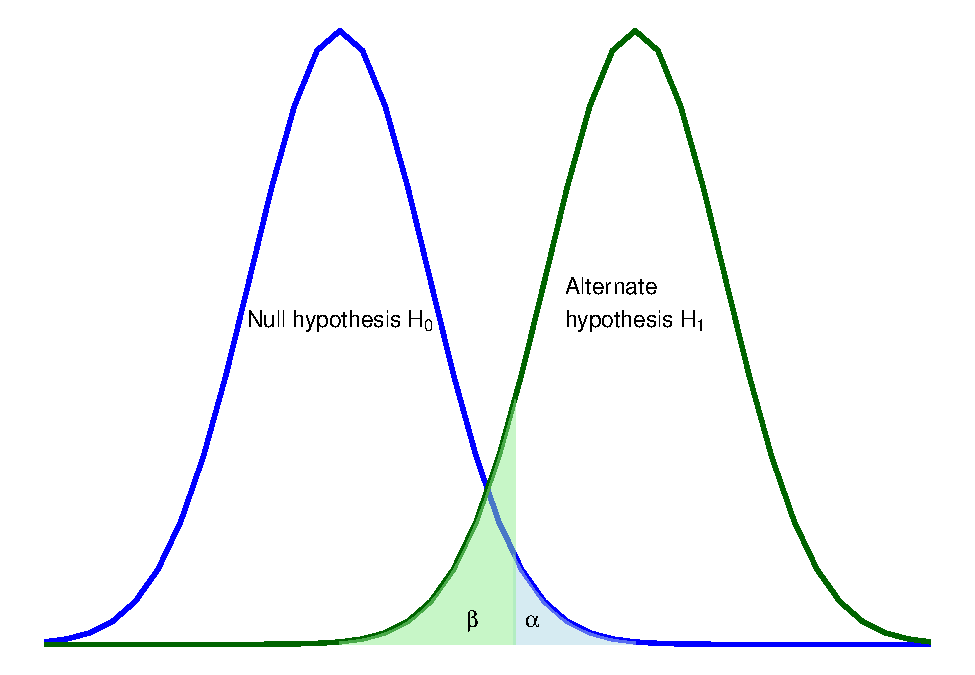
\includegraphics{_main_files/figure-latex/unnamed-chunk-83-1} \end{center}

The orange graph has most values very close to the peak at 50; therefore, the tails themselves are very small. The red line, on the other hand, is spread out and flatter so the tails are larger. The blue curve again approximates a normal distribution. We can quantify kurtosis through the idea of excess kurtosis - in other words, how far does it deviate from what we see in a normal distribution. This is shown below:

The different types of excess kurtoses are:

\begin{itemize}
\tightlist
\item
  Leptokurtic (heavy-tailed) - tails are smaller. Kurtosis \textgreater{} 1
\item
  Mesokurtic - normally distributed. Kurtosis is close to 0
\item
  Platykurtic (short-tailed) - tails are larger, and the peak is flatter. Kurtosis \textless{} -1
\end{itemize}

Therefore, in the example above the orange curve would be considered leptokurtic, while the red one would be platykurtic.

Below are a series of skewness and kurtosis values from three different data sets. For each:

\begin{itemize}
\tightlist
\item
  Determine if the data is skewed or not, and if so then what type of skew
\item
  Determine the type of kurtosis
\item
  Sketch a rough version of what this skew and kurtosis might look like (doesn't have to be perfect!)
\end{itemize}

\begin{tabular}{l|r|r|r}
\hline
 & Dataset A & Dataset B & Dataset C\\
\hline
Skewness & 0.3209 & 5.2934 & -3.1945\\
\hline
Kurtosis & -0.1023 & 10.9238 & -2.7263\\
\hline
\end{tabular}

\section{z-scores}\label{zscores}

The last major component of this week is about a really useful but important property of the normal distribution (which, as you may have guessed, is fairly important in statistics. The process of standardising data and calculating z-scores is one that we actually use a lot in statistics.

\newline

Let's briefly recap where we're at so far:

\begin{itemize}
\tightlist
\item
  We've covered basic descriptive statistics, such as means, standard deviations etc etc.
\item
  We've talked a bit about the normal distribution and its properties - specifically, that 95\% of your data lies within 1.96 SD either way of the mean
\end{itemize}

If you've got those concepts down, the rest of this page will be fairly straightforward.

\subsection{z-scores}\label{z-scores}

\textbf{z-scores} (z), sometimes called \textbf{standard scores}, are a measure that describe how many standard deviations a single data point is from the mean. If you recall the figure of the normal distribution from the previous page, notice how we quantify how much data is captured in terms of the number of standard deviations. z-scores are essentially this number - in other words, 95\% of your data lies between z = -1.96 and z = 1.96.

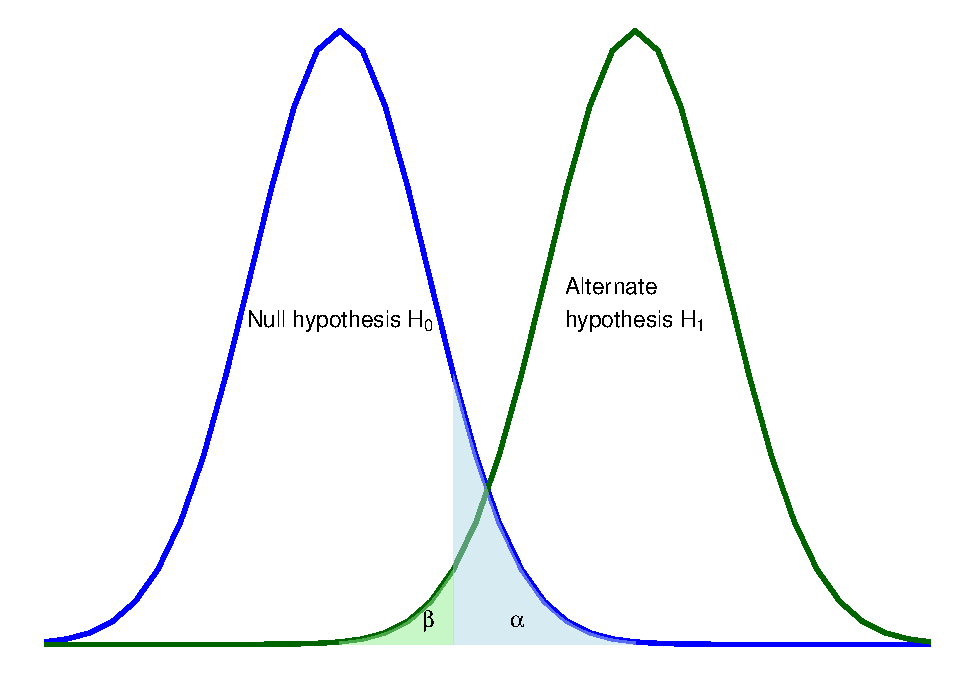
\includegraphics{_main_files/figure-latex/unnamed-chunk-85-1.pdf}

The process of calculating z-scores is called standardisation. The primary utility of converting data into z-scores is that it becomes possible to compare data on different scales. Many statistical analyses employ some form of standardisation for a variety of reasons - some of which we'll see in this subject.

\subsection{Calculating z-scores}\label{calculating-z-scores}

The formula for converting a raw data point into a z-score is:

\[
z = \frac{x - \mu}{\sigma}
\]

Where x = an individual data point, \(\mu\) = mean and \(\sigma\) = SD.

For example - in their paper on the Goldsmiths Musical Sophistication Index, Mullensiefen et al.~(2014) show that their general sophistication measure has a mean of 81.58, with an SD of 20.62. If a participant scores 100, we can calculate a z-score to see how many standard deviations they are away from the mean:

\[
z = \frac{100 - 81.58}{20.62}
\]
\[
z = 0.8933
\]
A participant with a general sophistication score of 100 would be roughly 0.89 standard deviations away from the mean.

To z-score a vector in R, we use the \texttt{scale()} function. The \texttt{scale()} function takes two arguments: \texttt{center}, which determines whether the data is centered (i.e.~subtracts the mean from each value), and \texttt{scale}, which essentially scales the data so the SD is 1. By default, both of these arguments are true.

\begin{Shaded}
\begin{Highlighting}[]
\FunctionTok{scale}\NormalTok{(vector\_a)}
\end{Highlighting}
\end{Shaded}

\begin{verbatim}
##            [,1]
## [1,]  0.3806935
## [2,] -1.3324272
## [3,]  1.5227740
## [4,] -0.7613870
## [5,] -0.1903467
## [6,]  0.3806935
## attr(,"scaled:center")
## [1] 3.333333
## attr(,"scaled:scale")
## [1] 1.75119
\end{verbatim}

\subsection{Comparing across scales}\label{comparing-across-scales}

As mentioned above, we can use z-scores to compare across measures on different scales. This becomes really useful when we want to compare two participants, for instance, or two different measures. This is simply done by calculating a z-score for each formula - as long as you know the mean and standard deviation of each scale as well.

As a simplistic example, let's say we have two scales:

\begin{itemize}
\tightlist
\item
  Measure A sits on a scale of 0 - 100, with a mean of 50 and a standard deviation of 5
\item
  Measure B sits on a scale of 0 - 80, with a mean of 45 and a standard deviation of 4
\end{itemize}

If a participant scores 40 on both scales, clearly we can't compare them directly - a 40/100 is vastly different to a 40/80! But we could convert these into z-scores to see where the participant sits on each scale:

\(z_a = \frac{40 - 50}{5}\), and \(z_b = \frac{40 - 50}{5}\)

\(z_a = \frac{-10}{5}\), and \(z_b = \frac{-5}{4}\)

\(z_a = -2, z_b = -1.25\)

In other words, the participant's z-score on Measure A is -2, and -1.25 on Measure B. Based on this, we can say that the participant scored slightly higher (relatively) on Measure B compared to Measure A.

A z-score lets us see how many standard deviations away from the mean a participant is. However, a more intuitive way of thinking about this is what percentile they sit in. To do this, we use something called a z-table. This z-table, in short, allows us to work out this percentage.

Most versions of the z-tables will present two separate z-tables: one for negative z-values, and one for positive z-values (credit: \url{https://zoebeesley.com/2018/11/13/z-table/})

\includegraphics{img/z-table.webp}

Here are the steps to read this table:

\begin{enumerate}
\def\labelenumi{\arabic{enumi}.}
\tightlist
\item
  Choose which table to read first. If you have a negative z-score, read the left one; if you have a positive z-score, read the right one.
\item
  The rows and columns are basically arranged by decimal place. The rows index z-scores to 1dp, while the columns add the second decimal place. So, find the row first that corresponds to your z-score. In our example from above, our z-score was 0.89, so we want to find the row corresponding to 0.8.
\item
  Next, find the column that corresponds to the second decimal place. We want to go all the way to the right-hand column labelled .09, to find the right column for our z-score of 0.89.
\item
  Find the cell that corresponds to the row and column from above - that is the probability of getting a value below our z-score.
\end{enumerate}

\begin{center}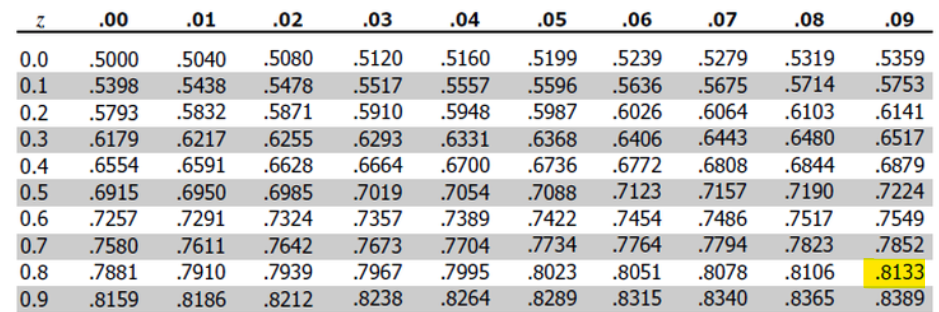
\includegraphics{img/ztable_highlight} \end{center}

In this instance, our z-score of 0.89 has an associated probability of .8133, meaning that 81.3\% of scores are below this z-score.

\chapter{Inferential statistics}\label{inferential-statistics}

From a conceptual point of view, this week's module might just be the most important that we cover in this subject. I don't say that to freak you out, but in many ways it just is the genuine truth. The reason that this might be the most important one is because the topics that we cover in this module are ones that many people frequently misunderstand or misappropriate - to the point of scientific fraud.

Inferential statistics are the subject of very heated debate in statistics, primarily about whether p-values and the like are really the right way to do science and statistics. We won't really go there because that's neither here nor there in terms of what the aim of this module really is: to not only show you one way of hypothesis testing, but to also equip you with the knowledge needed to understand how other people test hypotheses - or, sometimes, fail to do so.

Before you go into this module - make sure that you have 5.4 Variability, 5.5 Distributions and 5.6 Central Limit Theorem firmly under your belt as they will be relevant here.

By the end of this module you should be able to:

\begin{itemize}
\tightlist
\item
  Describe the steps taken to test a statistical null and alternative hypothesis
\item
  Correctly define a p-value
\item
  Explain the difference between Type I and Type II error, and how these relate to statistical power
\item
  Construct a basic confidence interval for a point estimate, and interpret it
\end{itemize}

\section{The logic of hypothesis testing}\label{the-logic-of-hypothesis-testing}

Central to all statistical testing is the underlying logic of hypothesis testing. All of the statistical tests that we cover in this module are built on this logic - and so it marks a great place for us to start our venture into inferential statistics.

\subsection{Revisiting the hypotheses}\label{revisiting-the-hypotheses}

In Module 4, you will have had the chance to write your own hypothesis. This hypothesis guides the overall research and methodological design of our studies. However, you may have noticed that the hypotheses discussed in the video are not quite in the same format. This is because `hypothesis' in this context refers to statistical hypotheses.

Statistical hypotheses are formal statements that we use when testing for an effect. As mentioned in the video above, we propose two contrasting hypotheses when we want to do statistical testing:

\begin{verbatim}
The null hypothesis (H0) - that there is no effect or difference
The alternative hypothesis (H1) - that there is an effect or difference
\end{verbatim}

We can never know for sure whether one hypothesis is correct over the other. Instead, we choose to either reject or not reject the null hypothesis.

\subsection{The issue of tails}\label{the-issue-of-tails}

There are two main types of alternative hypotheses:

\begin{itemize}
\tightlist
\item
  Two-tailed: we hypothesise that something is happening regardless of whether it's greater, smaller, increasing, decreasing etc\ldots{}
\item
  One-tailed: we hypothesise that the effect has a direction
\end{itemize}

In a two-tailed hypothesis, we predict that an effect is occuring but we don't predict anything beyond that. For example, if we are comparing whether two groups are different our alternative hypothesis would be that they are different - but we don't predict whether group A will be bigger than group B or vice versa. These are sometimes called non-directional hypotheses.

The blue areas on the curve on the right represent a 0.05 level of signifiance for a two-tailed hypothesis test. This is essentially how likely it is that we would observe our effect/difference if nothing was happening. If a difference is large enough that it falls within these blue tails, it is statistically significant. This is because if nothing really was happening, it would be unlikely that we see an effect/difference this big. Therefore, we would choose to reject the null hypothesis at this would fall below our chosen significance level.

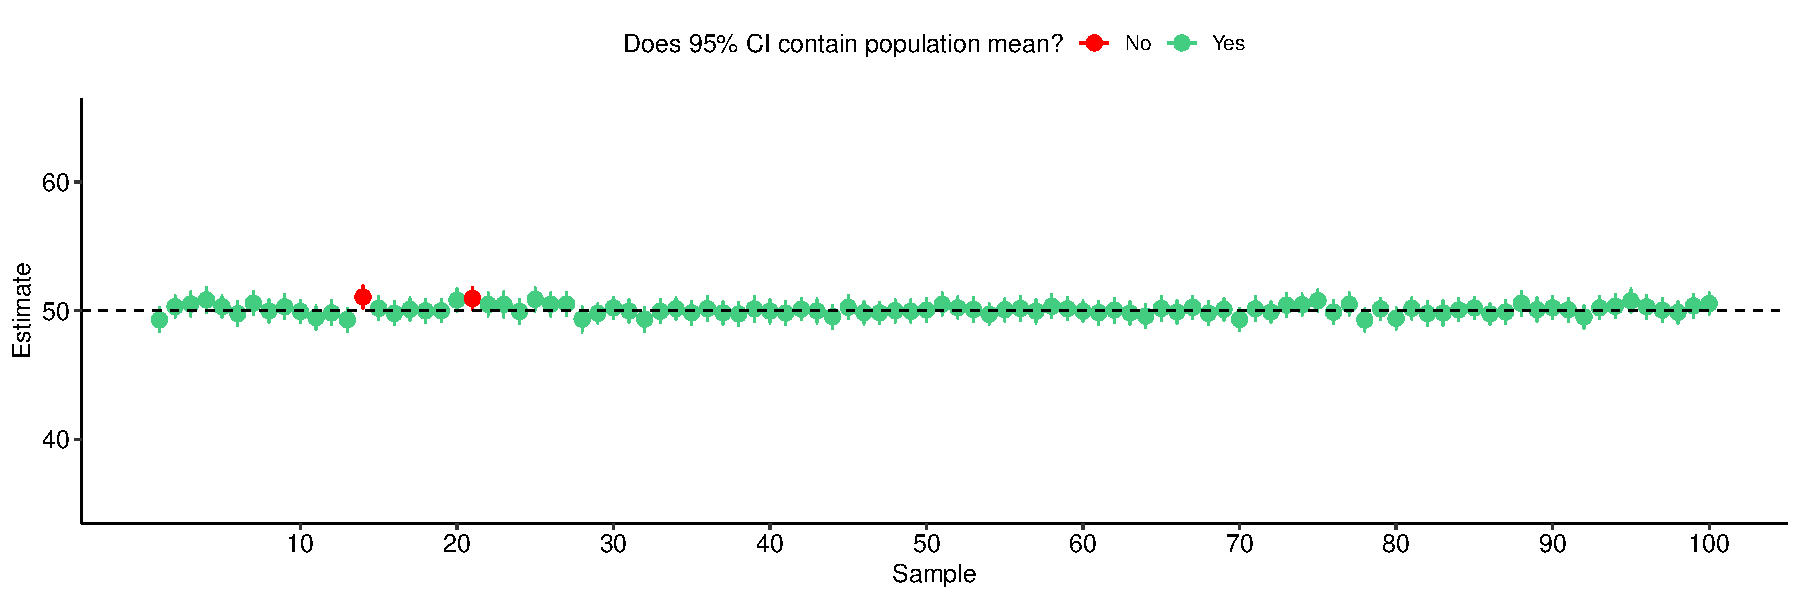
\includegraphics{_main_files/figure-latex/unnamed-chunk-90-1.pdf}

In a one-tailed hypothesis, we predict that the effect exists in a specific direction (hence, they are directional hypotheses). For example, we might predict that Group A is bigger than Group B. Or, we might predict that as X increases, Y increases too.

The two curves below show the significance levels for one-tailed hypotheses. If we predicted that Group A was smaller than Group B, we would only reject the null hypothesis if Group A really was smaller than Group B, and this difference was large enough to be statistically significant (i.e.~within one of the green tails).

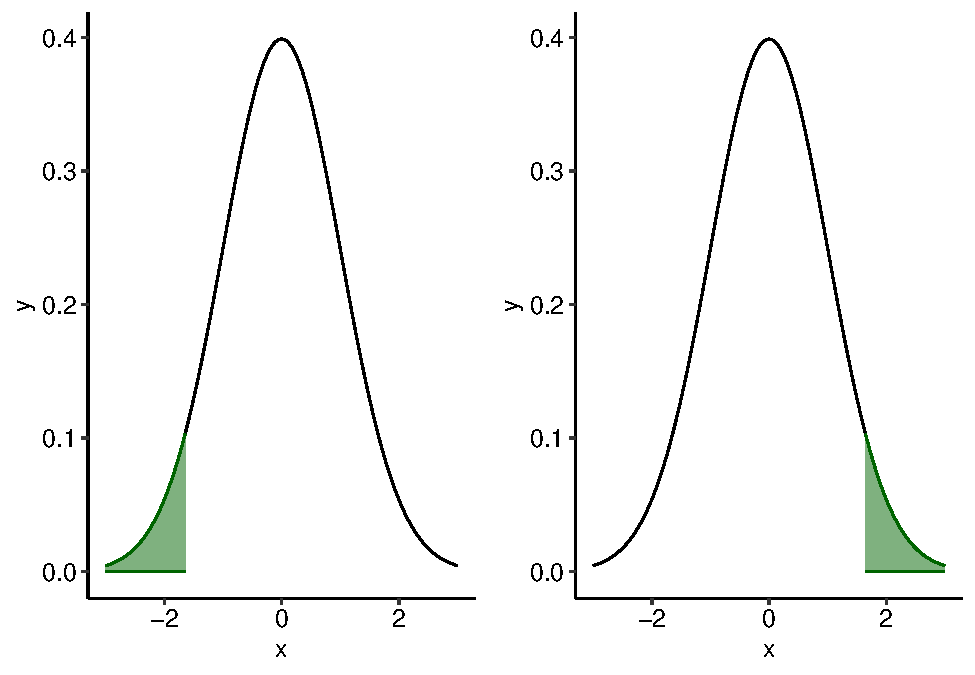
\includegraphics{_main_files/figure-latex/unnamed-chunk-91-1.pdf}

\section{p-values}\label{p-values}

At one point, the video on the previous page talks about `levels of significance' - what does this actually mean? Here, we'll talk about the p-value - one of the most commonly used, and possibly abused, concepts in research and statistics. We'll talk about what the p-value actually means, and tie it to two related concepts later in this module: error and statistical power.

\subsection{The definition of the p-value}\label{the-definition-of-the-p-value}

The definition of the p-value is the following (APA Dictionary, 2018):

\begin{quote}
``in statistical significance testing, the likelihood that the observed result would have been obtained if the null hypothesis of no real effect were true.''
\end{quote}

What does this actually mean? We actually already touched on this in the previous page, but let's dig a bit deeper.

\subsection{A brief probability primer, and how this relates to p-values}\label{a-brief-probability-primer-and-how-this-relates-to-p-values}

To start with, a p-value is a probability. A probability, of course, ranges from 0 to 1; 0 (0\%) representing an impossible result, and 1 (100\%) representing a certain result. Probabilities can be conditional, meaning that they are dependent on a certain condition being true. A p-value is a conditional probability. Specifically, a p-value refers to the probability of getting a particular result, assuming the null hypothesis. To illustrate what I mean, consider the two graphs below, showing some example data as points.

On the right is an example of what one possible alternative hypothesis might look like - that this data is meaningfully represented by two underlying distributions or groups, and that there is a difference between these two groups (shown as the blue and red curves). Contrast that with the left graph, where we hypothesise that there is no difference - in other words, that the data can be captured by the one distribution. This graph on the left is a representation of our null hypothesis, and as per the definition of the p-value, this is the distribution we focus on.

\includesvg{img/prob_dist.svg}

The area shaded blue represents the probability of getting that specific result. In the left example, the area shaded represents the probability of getting a value lower than x = 1. You can see that the blue area is quite big, so the probability of getting a value lower than 1 is quite high. On the right hand side is another example, which represents the probability of getting a value of x higher than 2. Here, the shaded area is small, so the associated probability is low.

Now, recall the following figure from last week:

\begin{center}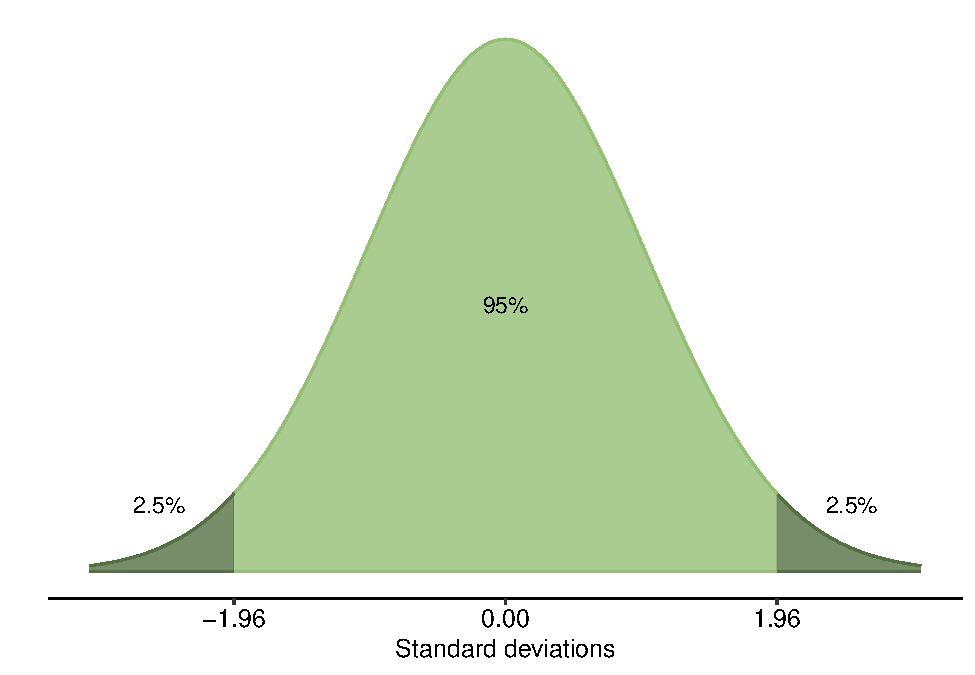
\includegraphics{_main_files/figure-latex/unnamed-chunk-93-1} \end{center}

We established last week that on a normal distribution, 95\% of the data lies within a certain range of values. Obtaining values beyond these thresholds (1.96 standard deviations either side of the mean) account for a relatively small percentage of possible values. In other words, the probability of getting a value beyond these bounds (in the figure above, where the dark green areas are) \textbf{is low}.

This is basically the thinking we use when we calculate a p-value. Let's break down the steps:

\begin{enumerate}
\def\labelenumi{\arabic{enumi}.}
\tightlist
\item
  We first \textbf{assume the null hypothesis is true}, and so we use the distribution of the null hypothesis to calculate the probability of getting our result or greater.
\item
  To figure out where our result(s) sits on this null distribution, we calculate a \textbf{test statistic}. This test statistic is essentially a value that represents where our data sits on the test (null) distribution. Each test statistic is calculated in a different way because every distribution looks different, so we'll come back to this over the next couple of weeks.
\item
  Afterwards, we calculate the probability of getting our test statistic (or greater) using a similar logic to the example above. This probability is our p-value. This marks the probability of observing this result or greater.
\item
  Once we have a p-value we then compare this against \textbf{alpha}, which is our chosen significance level (usually p = .05). If the probability of getting our result is smaller than this (pre-defined) cutoff, it means that it is unlikely assuming the null hypothesis is true, and therefore our result is statistically significant and we \textbf{reject the null hypothesis. }
\end{enumerate}

So in essence, if a p-value is p = .05 we're saying that assuming the null is true, there is a 5\% chance of observing this result or greater. Likewise, an extremely small p-value (e.g.~p = .0000000001) means that assuming the null is true, the probability of getting the data we have is extremely small. The logic, therefore, is that there must be an alternative explanation.

To clarify, the example above is just on a normal distribution - each statistical test we perform has its own (null) distribution, which we will talk about more in future modules. However, the rationale across tests is essentially the same.

\subsection{The debate around p-values}\label{the-debate-around-p-values}

Throughout history, p-values have been so misunderstood and misappropriated that some journals, such as Basic and Applied Social Psychology, actually either discourage or outright ban the reporting of p-values. This ties into a wider debate about the usefulness or meaningfulness of the hypothesis testing approach outlined on the previous page, with a number of academics and scientists arguing that it is time to do away with the system as a whole.

The debate is something that goes beyond the scope of the subject, so we won't be taking a strong stand on it either way. What we do think though is that it's really important that you understand how hypothesis testing works and what p-values can or can't tell you.

\section{Types of error}\label{types-of-error}

Nothing in life is perfect, and that applies to the inferential statistics that we do. Every sample will differ slightly from one to another due to inherent sampling error; in a similar way, whenever we do an inferential test about a population from a sample, we always run the risk of making an error in the decisions that we make.

\subsection{Statistical error}\label{statistical-error}

Imagine an old man is seeing his local GP complaining of a headache. Upon examination, the doctor concludes that the old man is pregnant.

A pregnant woman in her last trimester then comes in to the same GP. Despite her numerous pregnancy-related complaints, the doctor concludes that she is not pregnant.

Both of these scenarios (while hopefully very unlikely!) are obviously forms of errors on the doctor's part. In the first scenario, the doctor has accepted a diagnosis that is very clearly wrong. In the second scenario, the doctor has rejected the correct diagnosis.

The same kind of logic applies directly to quantitative research. We want to be sure that when we observe a result, that result is actually likely. We therefore want to minimise the possibility of errors like above.

We can draw a table to illustrate the possible outcomes when we perform a given hypothesis test:

\begin{tabular}{l|l|l}
\hline
 & Accept the null & Reject the null\\
\hline
The null is true & Correctly accept the null & Type I error\\
\hline
The alternative is true & Type II error & Correctly reject the null\\
\hline
\end{tabular}

\subsection{Type I error and alpha}\label{type-i-error-and-alpha}

A moment ago we talked about alpha (\(\alpha\)), or the significance level, from the previous sections about hypothesis testing and the p-value. Alpha is the same here as it is there - it is the probability of making a Type I error - that we incorrectly reject the null hypothesis when the null hypothesis is actually true. Essentially, alpha is the rate of Type I error we're willing to accept whenever we do a hypothesis test.

We generally set alpha as \emph{p} \textless{} .05 out of convention - i.e.~most of the time, we're willing to accept a 5\% chance of a Type I error rate. However, we can set alpha to anything we want. Sometimes, we may set it lower (more on this in a few weeks' time).

\section{Statistical power}\label{statistical-power}

Another related but crucial consideration for inferential statistics is the concept of statistical power. Without spoiling too much about what it means here, below is an overview of what this concept is and why it is important.

\subsection{Statistical power}\label{statistical-power-1}

Power in a statistical context essentially describes how likely we are to actually detect an effect given our sample size. Mathematically, power is defined as \(1 - \beta\), which in English terms means that it is the probability of not making a Type II error. Power is expressed as a percentage. For example, if your study has 50\% power, it means it has an 50\% chance of actually detecting an effect. The most common guideline is to aim for a study with 80\% power.

\subsection{Factors that affect power}\label{factors-that-affect-power}

The primary factor (within your control) that affects how much statistical power you have to detect an effect is sample size. Think back to the formula for standard error, as a proxy explanation as to why this is the case. Larger samples tighten the sampling distribution of the mean, and so two distributions will overlap less and less the greater the sample sizes are. Therefore, if there is less overlap there is greater space to detect an effect.

Some other factors that can affect power are:

\begin{itemize}
\tightlist
\item
  The effect size - how large is the difference between your groups, etc? If you're trying to detect very small effects, you need much more power to detect it compared to larger ones.
\item
  Performing a one-tailed test - because effects are only being tested in one direction, this alters the p-value (it actually halves it; a two-tailed p = .10 is a one-tailed p = .05). Don't do this though, because there are very few instances in which you can justify using a one-tailed test without reviewers and other clued-in readers suspecting that you're intentionally fudging your power.
\item
  Increase alpha - for a semi-detailed explanation of why, see here. In addition, there is a nifty tool here that lets you see what happens to error rates when you change specific parameters: Link to the tool
\end{itemize}

The consequence of being underpowered means that you can miss effects that exist. A good proportion of studies in psychology are underpowered, meaning that effects are being missed where they exist. Power is therefore an integral consideration of good study design, particularly for experimental contexts.

Consider two hypotheses - a null and an alternative hypothesis. As long as we sample a population, the two will always overlap (even if that overlap is really small).

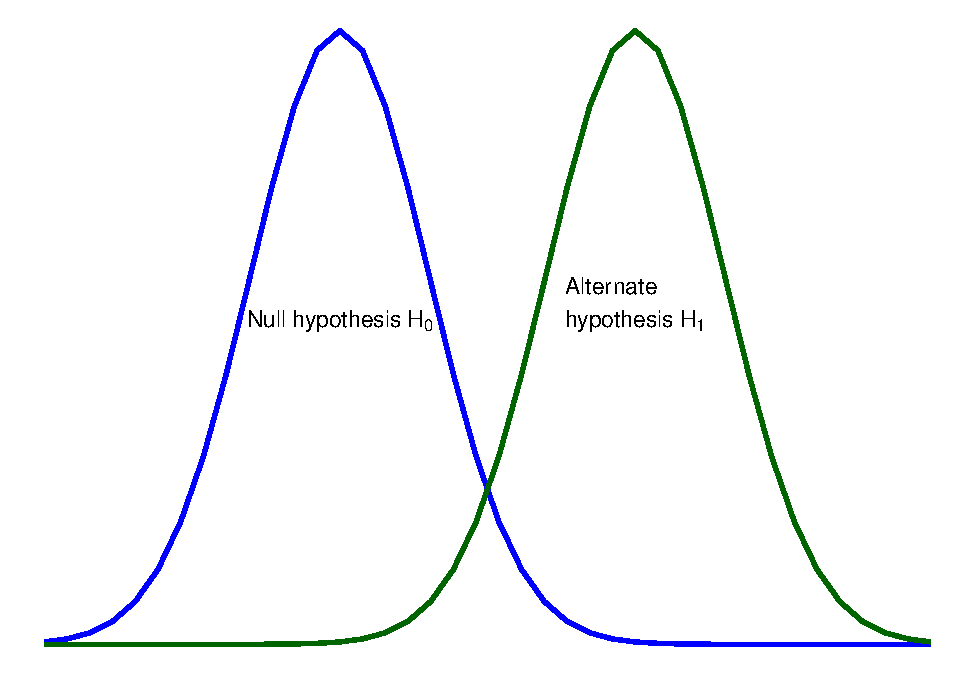
\includegraphics{_main_files/figure-latex/unnamed-chunk-95-1.pdf}

The area shaded in bright green below represents where the two distributions overlap with each other. This is where the null hypothesis might be rejected when it shouldn't be, or vice versa.

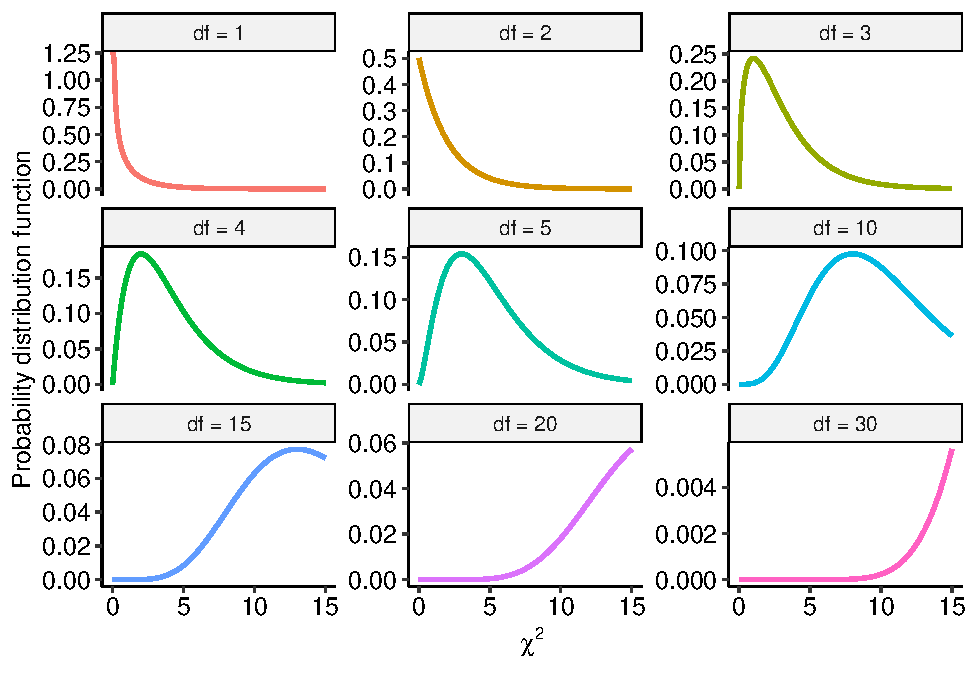
\includegraphics{_main_files/figure-latex/unnamed-chunk-96-1.pdf}
Let's assume an alpha of .05, and divide this region accordingly. There is a certain probability of alpha (where the null is incorrectly rejected), as well as a probability of beta (where the null is not rejected when it should be).

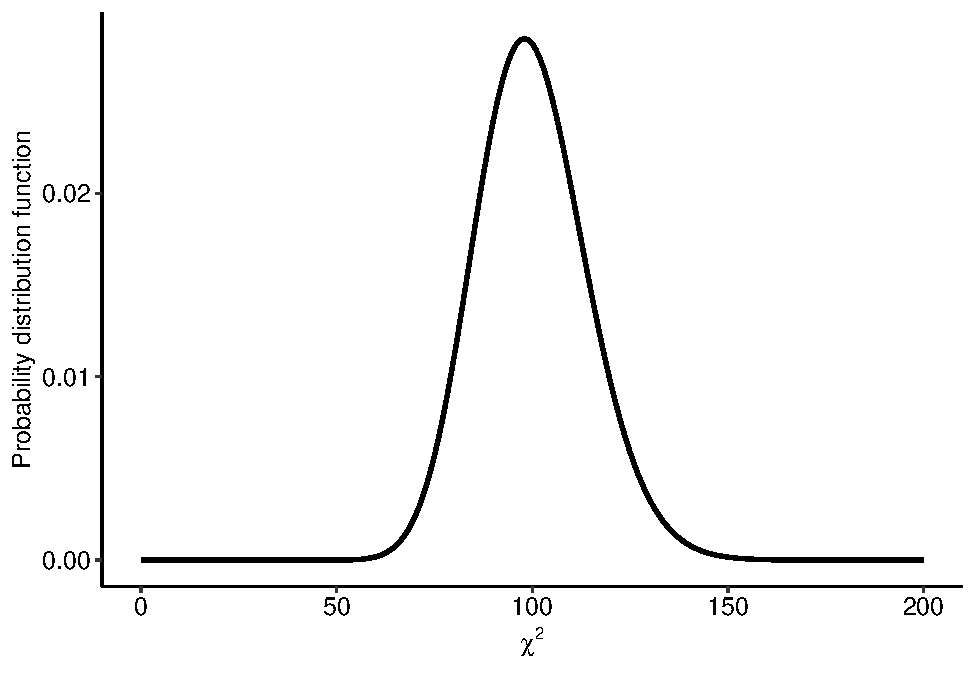
\includegraphics{_main_files/figure-latex/unnamed-chunk-97-1.pdf}

What happens if we were to decrease alpha? (i.e.~reduce our Type I error rate)? All else being equal (sample size, effect size etc), we can see that alpha now takes up less space in the overlapping area - and so, beta (Type II error) will increase.

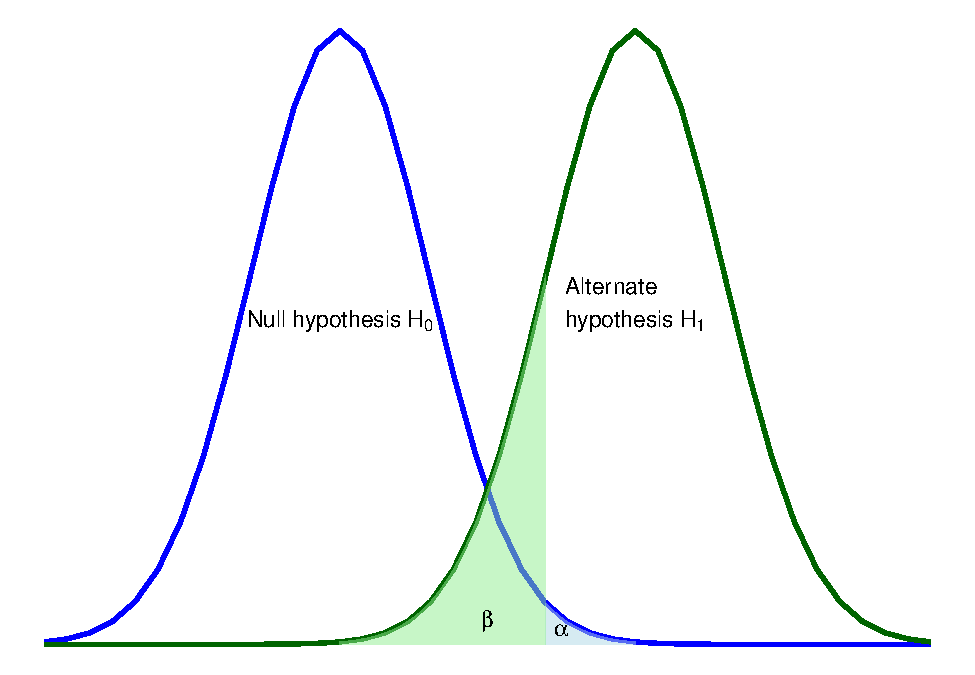
\includegraphics{_main_files/figure-latex/unnamed-chunk-98-1.pdf}

Subsequently, if we were to increase alpha we can see the opposite; beta will decrease, because now the overlap is predominantly now covered by the rejection region covered by alpha.

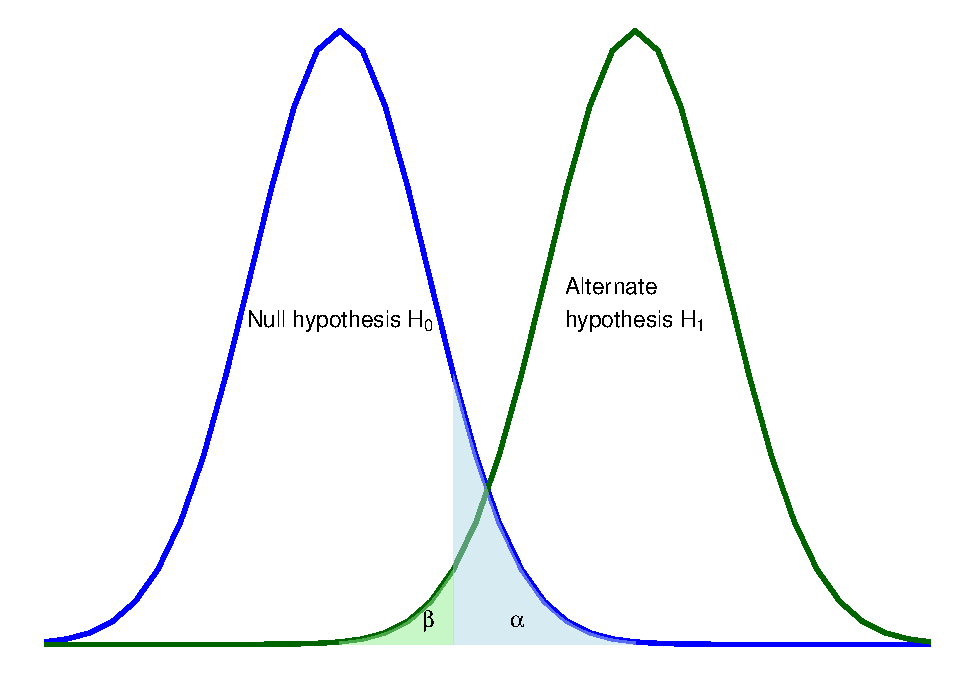
\includegraphics{_main_files/figure-latex/unnamed-chunk-99-1.pdf}

\subsection{Power analyses}\label{power-analyses}

Identifying an appropriate level of statistical power is an important part of planning quantitative research. Before conducting a study, it is wise to run a power analysis. Doing a power analysis allows you to identify how many participants you may need in order to reliably detect an effect of a given size.

Most modern statistics software will allow you to conduct power analyses:

\begin{itemize}
\tightlist
\item
  SPSS (from version 27)
\item
  Jamovi (with the jpower module)
\item
  R (with the \texttt{pwr} package, among many others)
\end{itemize}

We won't get too into the maths here of how this is done (it heavily depends on your research design, e.g.~how many groups you have, what test you plan on doing\ldots). These programs will let you select the appropriate design you want to test, and choose the size of the effect you want and your alpha level. The power analysis will then give you a minimum sample size per group for you to achieve that level of statistical power.

\subsection{Post-hoc power analyses}\label{post-hoc-power-analyses}

You might see authors in some papers where you present a power analysis after collecting your sample and doing your analyses. Supposedly, this is to show that your sample had enough power to detect an effect. However, this is conceptually flawed. The primary flaw is that post-hocs are essentially just restatements of your p-values and so do little to show the true power of a design/test.

\section{Confidence intervals}\label{confidence-intervals}

As we saw on the page about p-values, some people are vocal about their distaste for relying solely on p-values for decision making. One way of augmenting our estimates is to calculate a confidence interval for each estimate we make. Confidence intervals provide an estimate of the precision of our estimate, and so are a crucial concept to know about.

\subsection{A reminder from the previous module}\label{a-reminder-from-the-previous-module}

It's time to force you to remember what the graph below means once again (I promise this is the last time you will see this figure! I think). By now you should be very familiar with what this graph shows; namely, that 95\% of the data in a normal distribution lies within 1.96 standard deviations either side of the mean, yada yada.

\begin{center}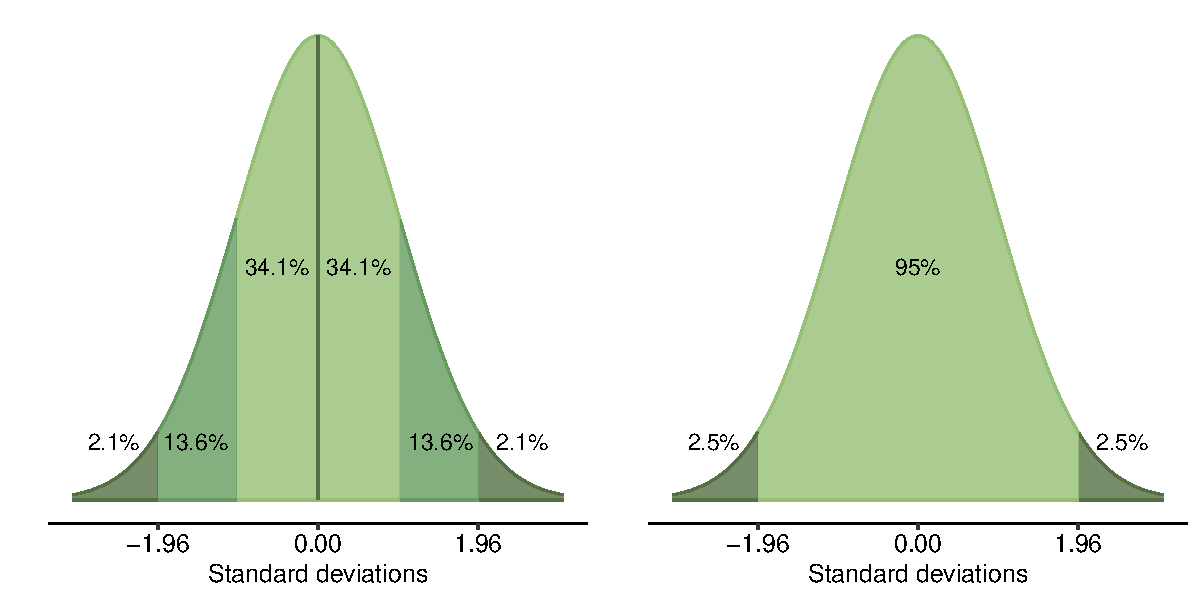
\includegraphics{_main_files/figure-latex/unnamed-chunk-100-1} \end{center}

This sounds all well and good, but this provides us with some useful information. If all that business about values within 1.96 standard deviations is still fresh in your mind, this next statement should be a no-brainer: if 95\% of our data on a normal distribution lies within 1.96 SD either side of the mean, that means that there is a certain range of values that 95\% of our data falls in.

For example, say we have a sample of scores on a test, with a mean of 70 and a standard deviation of 4. If we want to know where 95\% of the scores lie in this sample, we would do the following calculation:

Using this formula, we can calculate the values where 95\% of the data lie:

In other words, 95\% of our data in this sample lie between 62.16 and 77.84. The remaining 5\% of the sample lie above or below these values.

\subsection{Confidence intervals}\label{confidence-intervals-1}

We can use the same principle to make inferences about the true population parameter. When we take a sample, each one will have its own standard error (remember this reflects an estimate of the distance between the sample mean and the true population mean). If we were to repeatedly take samples, in the long run we would expect the true population mean to fall within 95\% of all sample means. And, just like the normal distribution, when we look at the sampling distribution of the means below, 95\% of all sample means will fall within 1.96 standard errors (thanks to the Central Limit Theorem).

\begin{center}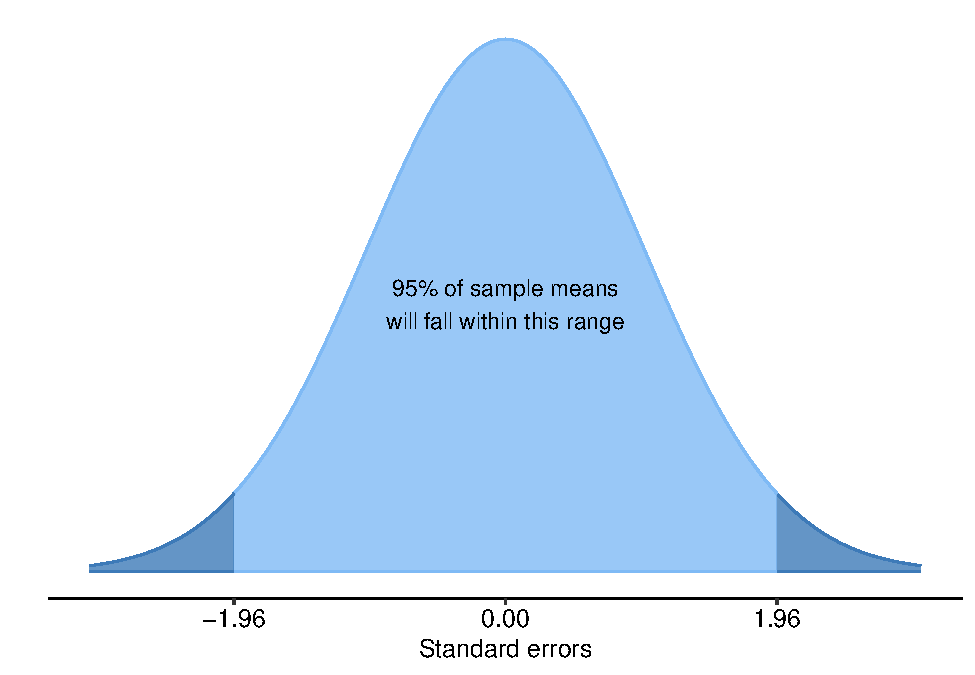
\includegraphics{_main_files/figure-latex/unnamed-chunk-101-1} \end{center}

With this important property in mind, we can calculate a 95\% confidence interval. This is an estimate of the range of values for our estimate of the parameter. In other words, it is a measure of precision. The formula for a 95\% confidence interval, as it turns out, is exactly the same as above with one change:

\[
95\% CI = M \pm (1.96 \times SE)
\]

Therefore, if we have an estimate of a population parameter (e.g.~what the population mean is), we can use a 95\% CI around that estimate to quantify the precision/uncertainty of that estimate. If a confidence interval is narrow, it suggests our estimate is quite precise.

This can be extremely informative at a glance. For example, pretend that we have a null hypothesis that a parameter is equal to 0 (as is usually the case). If we calculate a confidence interval and that happens to include the value of 0 (e.g.~95\% CI: {[}-0.5, 1.5{]}), we can immediately infer that 0 is a likely value for this parameter - and thus, the null hypothesis is plausible. On the other hand, if the CI did not include 0 then we could infer that there likely is a significant effect.

Not all confidence intervals though will contain the true parameter purely because of how samples work (i.e.~the inherent error between a sample and a population). In addition, it does not mean that there is a 95\% chance a single interval will contain the true parameter. So what does the 95\% part refer to?

\subsection{Confidence}\label{confidence}

The confidence level is a long-run probability that a group of confidence intervals will contain the true population parameter. A 95\% confidence level means that if we were to take samples repeatedly and calculate a CI for each one, 95\% of those CIs will contain the true population parameter in the long-run.

Or, say if you were to take 100 samples and calculate a CI for each one, 95 of them would include the true population parameter:

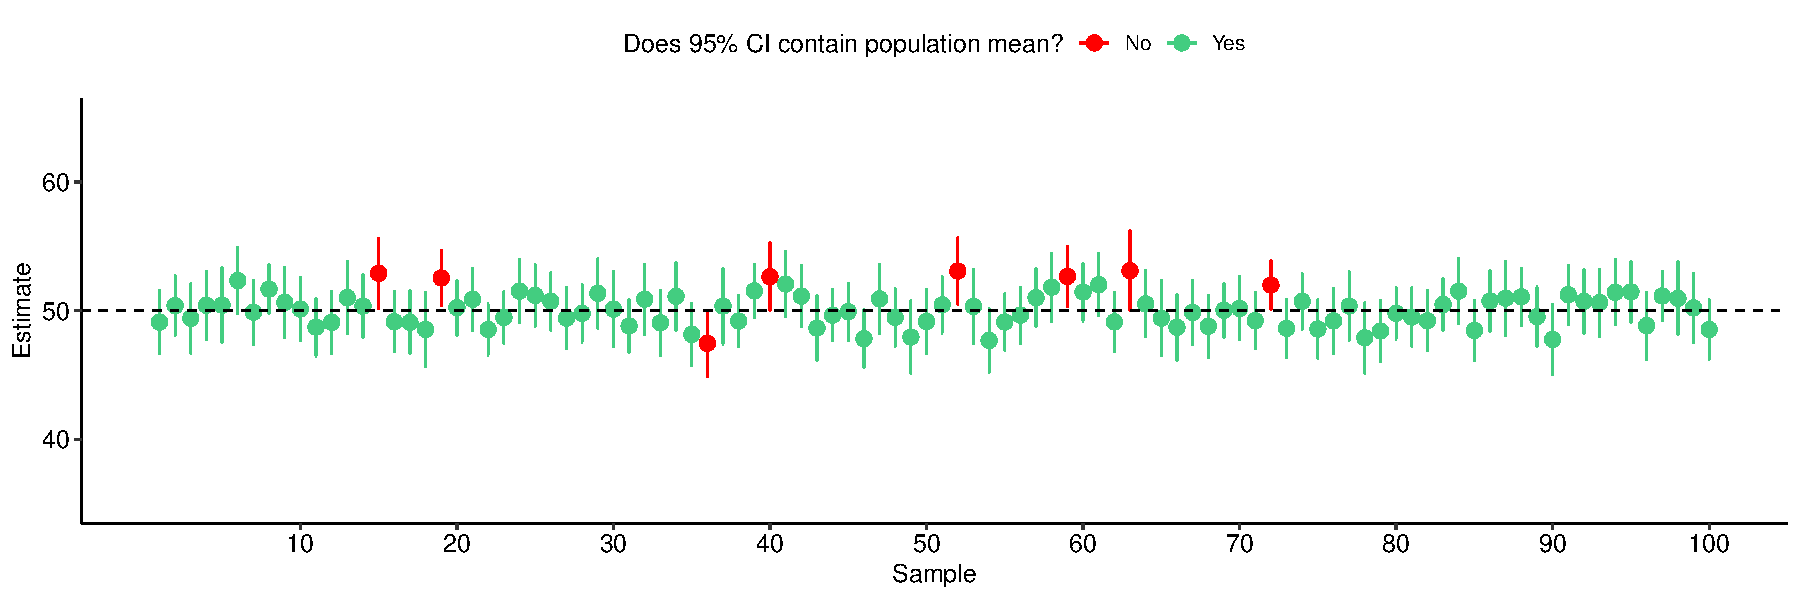
\includegraphics{_main_files/figure-latex/unnamed-chunk-103-1.pdf}

The 95\% long-run probability \textbf{does not change} with sample size. What does change, however, is the \textbf{precision} of the estimates. This makes sense if you remember the formula for standard error, which divides by the square root of \emph{n}. A larger \emph{n} will lead to lower SE, and thus narrower confidence intervals. Below is an example with a much larger sample size. Notice how the confidence intervals are now much smaller:

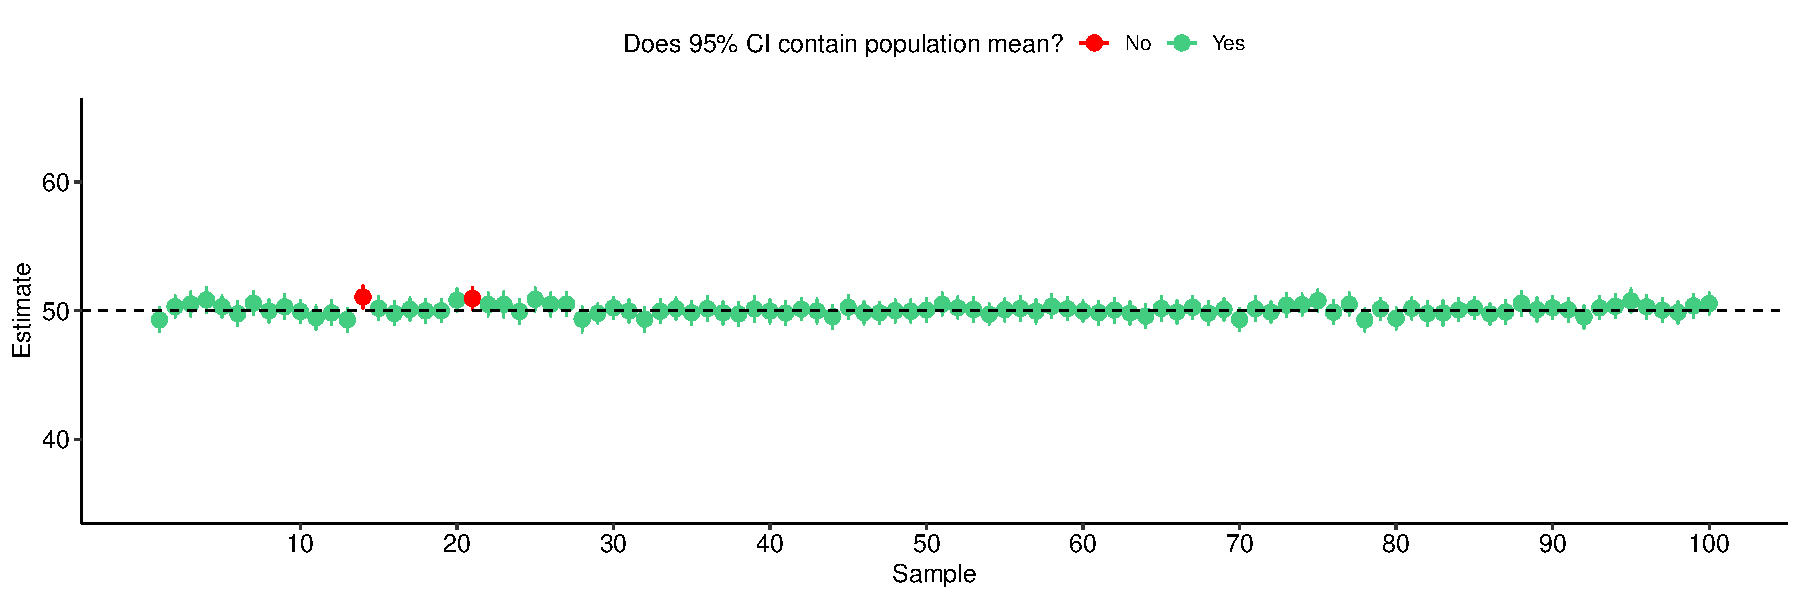
\includegraphics{_main_files/figure-latex/unnamed-chunk-104-1.pdf}

The choice of 95\% is conventional, like alpha (our significance criterion); we can (but often don't) change our level of confidence. This changes the relevant formula for calculating the interval, as in the examples below:

\[
90\% CI = M \pm (1.645 \times SE)
\]

\[
99\% CI = M \pm (2.576 \times SE)
\]

Notice that the value we multiply the SE by has changed. If you have been especially observant so far, you may have figured out what these values are: they're z-scores!

\subsection{Confidence intervals in literature}\label{confidence-intervals-in-literature}

On the page about p-values, I left a brief note around some of the current discourse around the usefulness (or uselessness) of p-values. Proponents of getting rid of p-values/moving away from them advocate strongly for two alternatives: a) effect sizes (self-explanatory; we will come to this) and b) confidence intervals, to show the range of long-run plausible values for the estimate.

Again, we won't be taking an especially strong stance either way. That being said, it is now fairly common practice to report 95\% confidence intervals alongside the results of significance tests for transparency. Programs like Jamovi will usually calculate these intervals automatically for you.

\part{Basic inferential tests}\label{part-basic-inferential-tests}

\chapter{Chi-squares}\label{chi-squares}

While many of the things we are interested in when it comes to psychological research are continuously distributed (height, weight, reaction time, personality), there are many instances where we will need to work with data that is categorical. This can involve categorical independent variables (e.g.~assigning participants to one or two groups) or categorical outcomes (e.g.~responding yes or no). We'll start with looking at relationships between these categorical variables, and testing for significant associations.

This module will see you diving deep into Jamovi again - so be prepared to get hands on with a bunch of data! Between the seminar, the worked examples and exercises there are at least 6 different datasets to play around with for this week!

By the end of this module you should be able to:

\begin{itemize}
\tightlist
\item
  Describe how a chi-square statistic is calculated
\item
  Conduct two forms of chi-square tests: goodness-of-fit and tests of independence
\item
  Calculate and interpret an appropriate effect size for tests of independence
\end{itemize}

\begin{figure}

{\centering \includegraphics{https://imgs.xkcd.com/comics/question_2x} 

}

\caption{[xkcd: Question](https://xkcd.com/1448/)}\label{fig:unnamed-chunk-107}
\end{figure}

\section{Calculating a chi-square}\label{calculating-a-chi-square}

We'll start this module off by briefly going through the basics of what research designs suit chi-square tests, as well as the basic maths underlying the first part of the statistical test.

\subsection{Categorical data}\label{categorical-data}

As mentioned at the start of this module, chi-square tests are used when we work with \textbf{categorical data} - i.e., when we are dealing with \emph{counts} of items or people, rather than continuous variables. Research questions focused on relationships or associations among categorical variables are suited to chi-square tests.

Every categorical variable will have \textbf{levels} (categories) within them. These are the different values that categorical variable can be. For example, biological sex is often coded with two levels: male and female. Or perhaps you might categorise socioeconomic status into three levels: low, medium and high bands. This is something that can form a core part of your research design. The most basic example is asking participants what their biological sex is - participants will respond with one of the two categories.

Alternatively, you can \emph{create} categories from existing data. For example, many scales designed to assess psychological disorders such as depression and anxiety often have `cutoff' points, where a certain score on the scale is indicative of a possible disorder. If you have everyone's raw scores, you can convert these scores into categories depending on whether they are above or below these cutoff points (though this needs to be strongly justified).

All of this kind of data are amenable to chi-square tests, \emph{if} you are interested in relationships between categorical variables. The family of chi-square tests basically work by comparing the \textbf{observed values to} the \textbf{expected values}. As the names imply, observed value simply means the number of observations we have in each category or level (i.e.~what our data actually is). Expected values, on the other hand, are the number of things we would \emph{expect} to see under the null hypothesis.

We can visualise categorical variables in two basic ways: a) a \textbf{contingency table} or b) a \textbf{bar graph of counts}. Below is the same set of data, shown in both forms:

\subsection{The chi-square formula}\label{the-chi-square-formula}

To test whether a result is significant, remember that we need to calculate a test statistic, and see where that fits on its underlying distribution. Here, our test statistic is handily named the \textbf{chi-square statistic}. To calculate the chi-squared test statistic we use the following formula:

\[
\chi^2 = \Sigma \frac{(O-E)^2}{E}
\]

Where:

\begin{itemize}
\item
  O = \textbf{observed value}
\item
  E = \textbf{expected} \textbf{value}
\end{itemize}

The English translation of that above formula can be described in four steps:

\begin{enumerate}
\def\labelenumi{\arabic{enumi}.}
\item
  Calculate observed count - expected count
\item
  Square that difference
\item
  Divide it by the expected count
\item
  Do this for each cell, and add them all up
\end{enumerate}

We'll look at this in more detail when we look at the actual tests. For the time being, here's the key takeaway: have a look at the two graphs below, representing the observed and expected values of two different datasets.

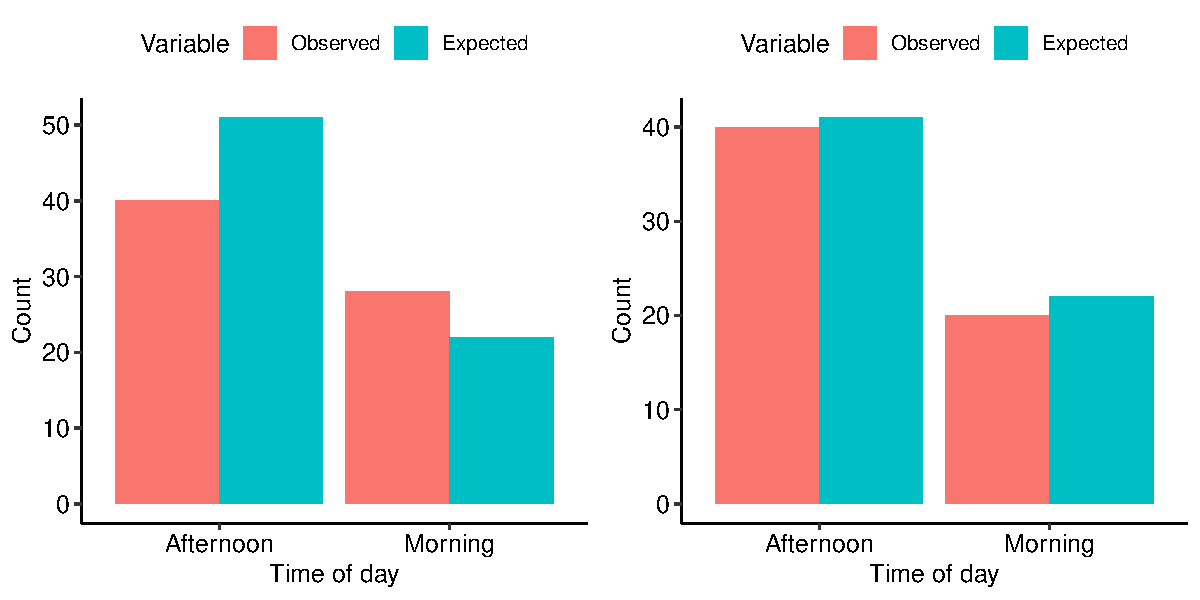
\includegraphics{_main_files/figure-latex/unnamed-chunk-108-1.pdf}

Have a think about the following:

\begin{enumerate}
\def\labelenumi{\arabic{enumi}.}
\item
  What is each graph telling you?
\item
  The left graph appears to show noticeable differences between the observed and expected values. Based on the mathematical formula above, what will happen to the chi-square value?
\item
  Each graph represents one set of data. Based on your answers to a) and b) above, which one of the two would you expect to demonstrate a significant effect?
\end{enumerate}

\section{The chi-square distribution}\label{the-chi-square-distribution}

On the previous page we introduced the formula for a chi-square test statistic. But what do we do with it? We'll go through this below in detail, given that this is the first time we're coming across an actual test. While a computer will do all of this stuff automatically, it's useful to know the actual mechanisms underlying the test.

\subsection{The chi-square distribution}\label{the-chi-square-distribution-1}

Recall from Week 6 about how hypothesis tests work - we calculate a test statistic that conforms to a particular distribution, and we assess how likely our observed test statistic is (or greater) on this distribution, assuming the null hypothesis is true. This gives us the p-value for that test. With that in mind, the chi-square distribution that underlies the chi-square test looks something like this:

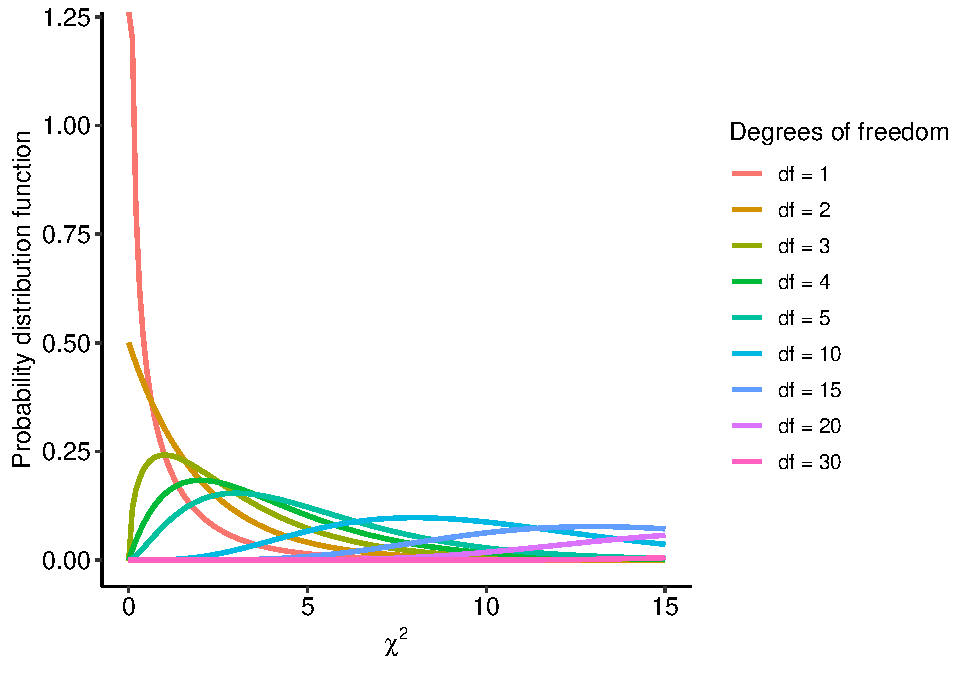
\includegraphics{_main_files/figure-latex/unnamed-chunk-109-1.pdf}

The shape of the chi-square distribution is only dependent on the degrees of freedom (\emph{df}). We'll look at how to calculate degrees of freedom for various tests, including the family of chi-square tests, as we move along the subject.

Here is the same set of lines above, but shown in their own plot this time:

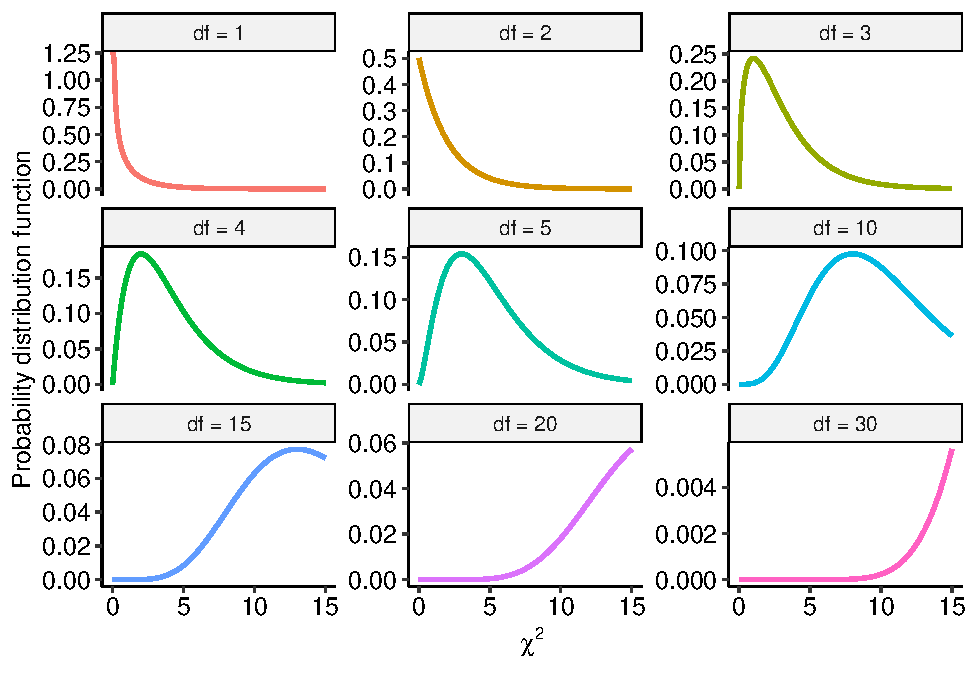
\includegraphics{_main_files/figure-latex/unnamed-chunk-110-1.pdf}

As you can hopefully see, the chi-square distribution is very heavily skewed at lower degrees of freedom (and therefore in smaller sample sizes). As degrees of freedom increase though, it approximates a normal distribution. For instance, here's what the chi-square distribution looks like when \emph{df} = 100:

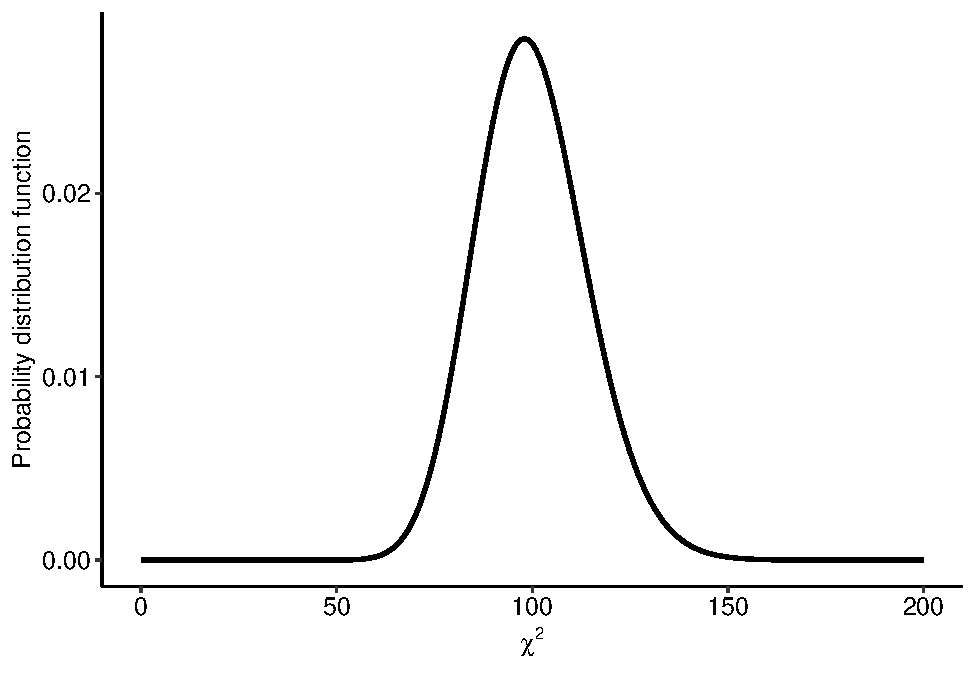
\includegraphics{_main_files/figure-latex/unnamed-chunk-111-1.pdf}

\subsection{Hypothesis testing in chi-squares}\label{hypothesis-testing-in-chi-squares}

At this point, also recall that \emph{p}-values are the probability that we would get our observed result (or greater), assuming the null hypothesis is true.

Here is our first application of this concept. When we use a chi-square test, we are performing the following basic steps:

\begin{enumerate}
\def\labelenumi{\arabic{enumi}.}
\tightlist
\item
  Establish null and alternative hypotheses
\item
  Determine alpha level (in this case, \(\alpha\) = .05 as always)
\item
  Calculate our test statistic - here, this is the chi-square statistic
\item
  Compare our chi-square test statistic against the chi-square distribution
\item
  Calculate how likely we would have seen our chi-square value or greater on this distribution
  a. Or, alternatively, establish a critical chi-square value - the value that must be crossed for a result to be significant
\end{enumerate}

We'll expand on this more in the next couple of pages.

\subsection{Calculating significance}\label{calculating-significance}

Let's say that we have a \emph{df} of 5. How do we know where the critical chi-square value is?

For that, we consult a chi-square table. This table gives the critical chi-square value at a set degrees of freedom and alpha level. These are freely available online, but here's a short excerpt. To read this table:

\begin{itemize}
\tightlist
\item
  The far-left column lists different degrees of freedom. We need to find the row that corresponds to \emph{df} = 5.
\item
  Each column provides critical chi-squares at different alpha levels. We want to find the column that says .05.
\item
  The number at both of these points tells us the critical chi-square value.
\end{itemize}

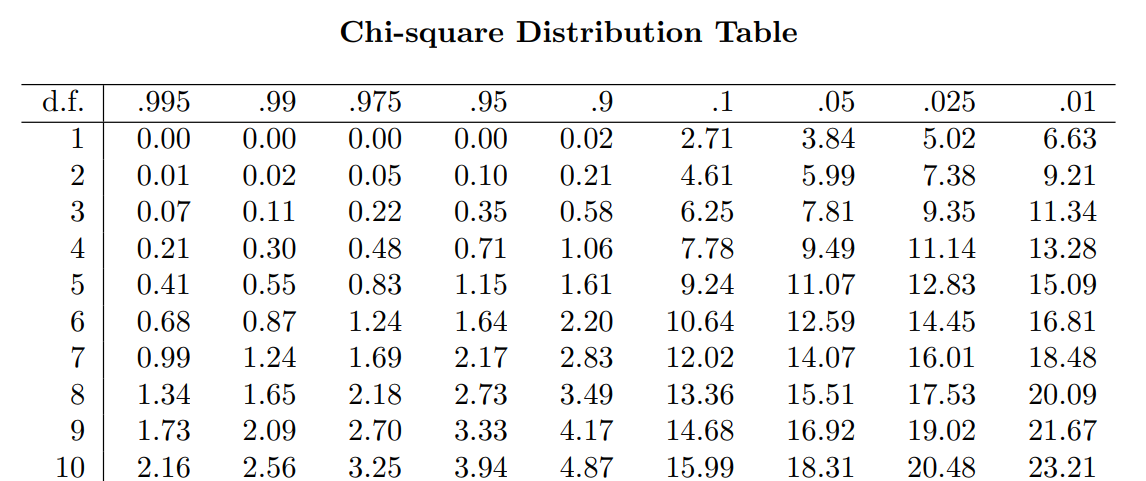
\includegraphics{img/w7_chisq_table.png}

So, for a \emph{df} = 5 and an \(\alpha\) = .05, the critical chi-square value is 11.07. If our own chi-square value is greater than this, the probability of that value or greater occurring (assuming the null) will be less than 5\%; i.e.~the boundary for statistical significance.

In picture form:

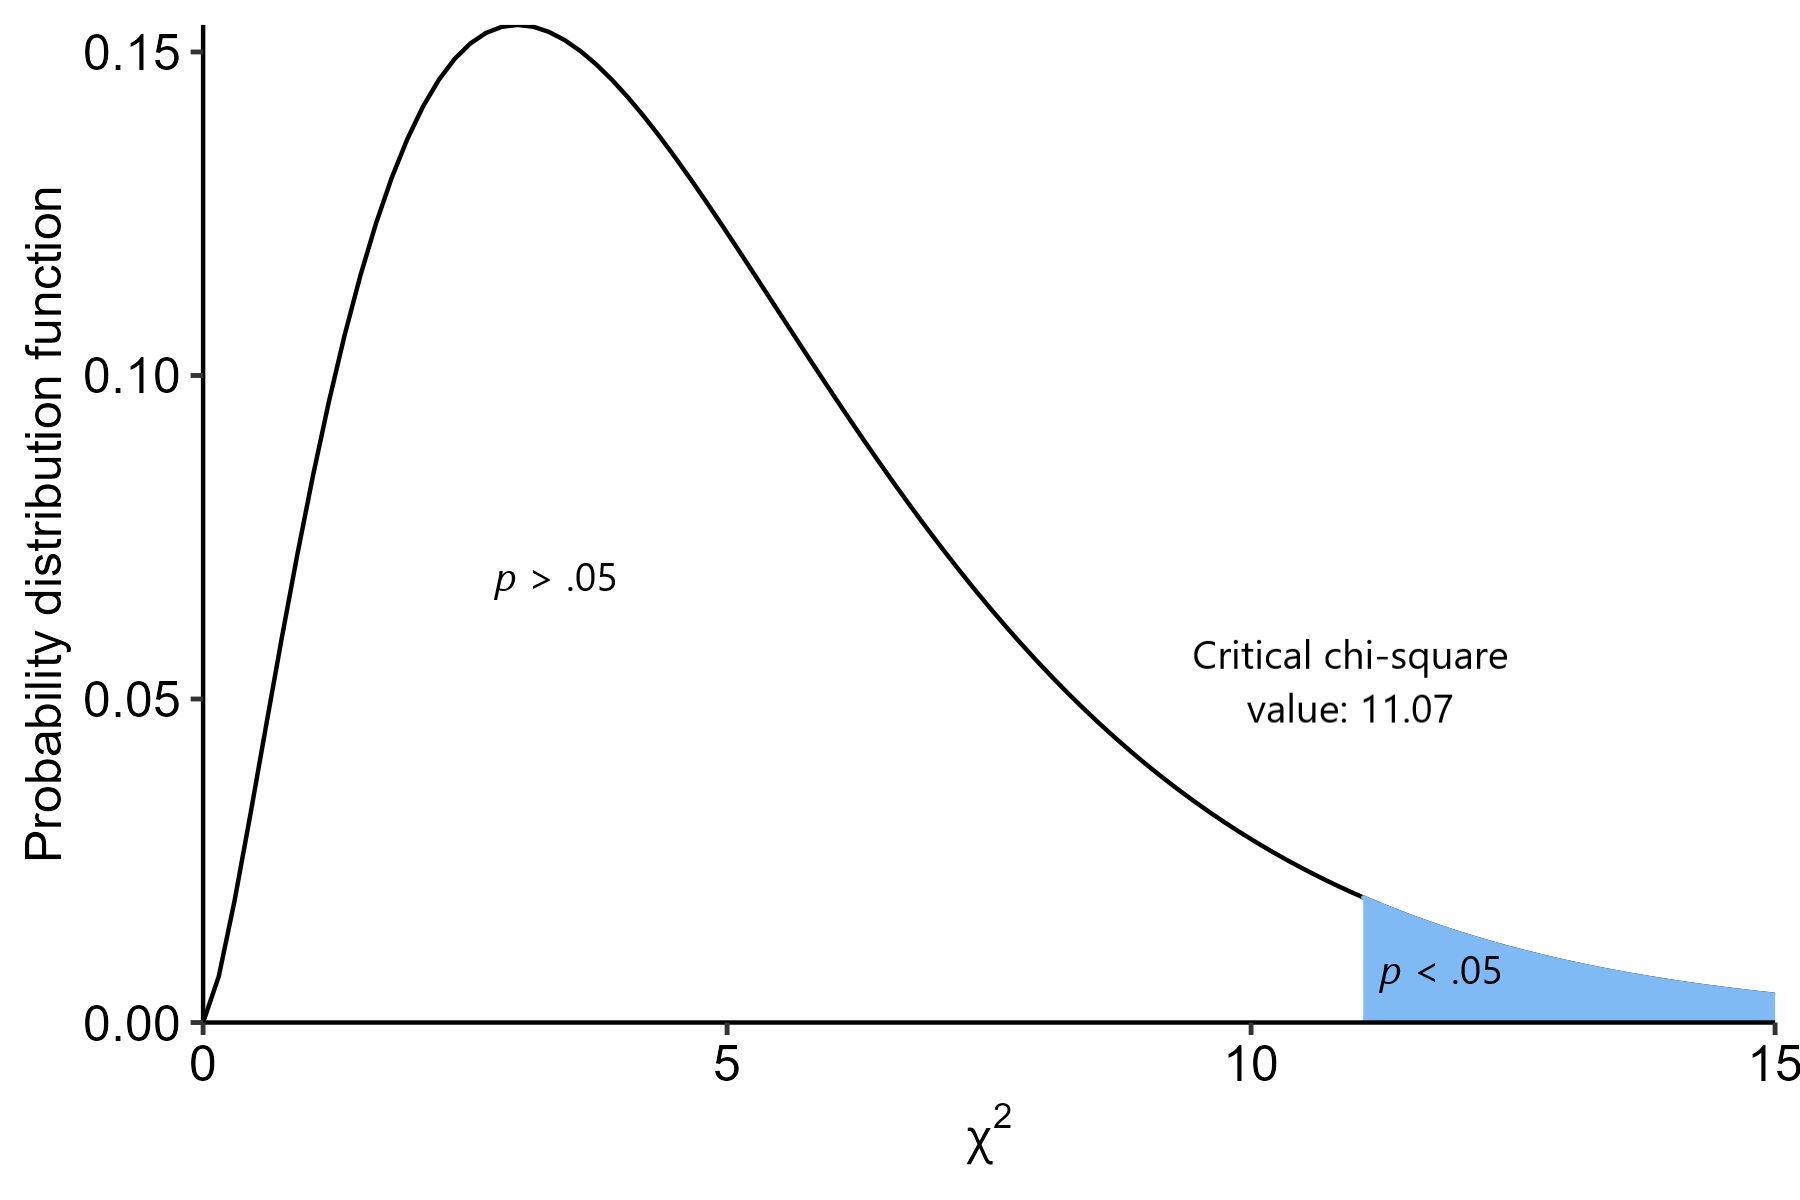
\includegraphics{img/w7_chisq_df_5.png}

Hopefully that makes sense - this kind of logic is pretty much identical to the other tests that we will cover in the coming weeks!

\section{Goodness of fit}\label{goodness-of-fit}

Now that we've covered the conceptual groundwork for chi-square tests in general, we can now start looking at actual tests that can help us answer research questions. The most basic chi-square test is the goodness of fit test.

\subsection{Goodness of fit tests}\label{goodness-of-fit-tests}

Goodness of fit tests are used when we want to compare a set of categorical data against a hypothetical distribution. Goodness of fit tests require one categorical variable - as the name implies, a goodness of fit test looks at whether the proportions of categories/levels in this variable fits an expected distribution. In other words, do our counts for each category match what we would expect under the null?

``Distribution'' in this context means probability distributions, and can apply to a wide range of scenarios. For the purposes of what we're learning here, we'll stick to a question along the lines of: ``do the categories of variable X align with their expected probabilities''?

\subsection{Example}\label{example}

An example question that we look at in the seminar is Do Skittle bags have an even number of each colour? In the seminar, we go through whether or not a random bag has an even split of colours.

Here on Canvas, we'll now tackle their equally delicious rivals, M\&Ms.~The data and analysis come courtesy of Rick Wicklin, a data analyst at SAS (who also make statistics software). You can read his full blog here: \href{https://blogs.sas.com/content/iml/2017/02/20/proportion-of-colors-mandms.html}{The distribution of colors for plain M\&M candies}. We'll be recreating Rick's first analysis here. We're sticking with the candy theme because a) they're delicious and b) the M\&Ms are a great way to introduce what to do when expected proportions are not equal.

M\&Ms come in six colours: red, blue, green, brown, orange and yellow. Unlike Skittles, these colours are not distributed equally within each bag of M\&Ms.~In 2008, Mars (the parent company) published the following percentage breakdown of colours:

\begin{itemize}
\tightlist
\item
  13\% red
\item
  20\% orange
\item
  14\% yellow
\item
  16\% green
\item
  24\% blue
\item
  13\% brown
\end{itemize}

Rick collected his data in 2017, and so was interested in seeing if the proportions observed in his 2017 sample of M\&Ms aligned with the distribution of colours listed in 2008.

A goodness of fit is the perfect test for this scenario because:

\begin{itemize}
\tightlist
\item
  We are making a claim about a distribution
\item
  Our variable (colour) is categorical
\item
  A chi-square goodness of fit will allow us to test whether the distribution of colours in a sample of M\&Ms aligns with the published proportions.
\end{itemize}

Here's our dataset:

\begin{Shaded}
\begin{Highlighting}[]
\NormalTok{mnm\_data }\OtherTok{\textless{}{-}} \FunctionTok{read\_csv}\NormalTok{(}\FunctionTok{here}\NormalTok{(}\StringTok{"data"}\NormalTok{, }\StringTok{"week\_7"}\NormalTok{, }\StringTok{"W7\_M\&M.csv"}\NormalTok{))}
\FunctionTok{head}\NormalTok{(mnm\_data)}
\end{Highlighting}
\end{Shaded}

\begin{verbatim}
## # A tibble: 6 x 2
##      id colour
##   <dbl> <chr> 
## 1     1 Red   
## 2     2 Red   
## 3     3 Red   
## 4     4 Red   
## 5     5 Red   
## 6     6 Red
\end{verbatim}

\subsection{\texorpdfstring{Calculating \(\\\chi^2\)}{Calculating \textbackslash\textbackslash\textbackslash chi\^{}2}}\label{calculating-chi2}

In goodness of fit tests, we first calculated the expected frequencies. In this example though, the expected proportions aren't equal - and so we have to be mindful of this when calculating expected values. See the expected count cell for Red M\&Ms for how expected value is worked out in this instance.

We can draw this up in table form alongside our own data:

\begin{tabular}{l|r|r|l}
\hline
Colour & Observed & Expected proportion & Expected count\\
\hline
Blue & 133 & 0.24 & 170.88\\
\hline
Brown & 96 & 0.13 & 92.56\\
\hline
Green & 139 & 0.16 & 113.92\\
\hline
Orange & 133 & 0.20 & 142.4\\
\hline
Red & 108 & 0.13 & $712 \times 0.13 = 92.56$\\
\hline
Yellow & 103 & 0.14 & 99.68\\
\hline
\end{tabular}

Then we would use the formula we saw on the previous page to calculate a chi-square statistic. However, since we're doing this in R we'll skip the manual maths.

\[
\chi^2 = \Sigma \frac{(O-E)^2}{E}
\]

If we have a look at the observed vs expected values, we might have a good idea of what's going on already:

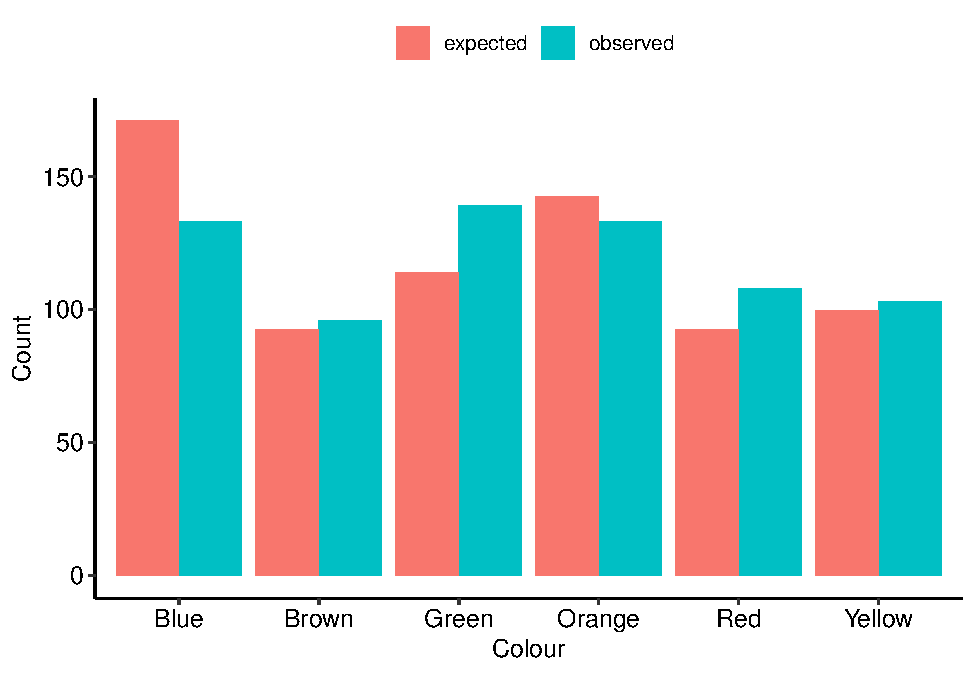
\includegraphics{_main_files/figure-latex/unnamed-chunk-116-1.pdf}

\subsection{Using R}\label{using-r}

Using Jamovi

By default, the \texttt{chisq.test()} function in R will assume that your categories have an equal chance of happening. However, in this instance we know that the colours are not evenly distributed. To ensure the proper probabilities are set beforehand, this needs to be specified by giving the \texttt{p} argument within \texttt{chisq.test()}. Note that the order of the expected probabilities needs to match the order they appear in the dataset (R will generally order these alphabetically unless told otherwise):

\begin{Shaded}
\begin{Highlighting}[]
\CommentTok{\# This pulls the relevant variable directly}
\NormalTok{w7\_mnm\_table }\OtherTok{\textless{}{-}} \FunctionTok{table}\NormalTok{(mnm\_data}\SpecialCharTok{$}\NormalTok{colour)}

\NormalTok{w7\_mnm\_chisq }\OtherTok{\textless{}{-}} \FunctionTok{chisq.test}\NormalTok{(w7\_mnm\_table, }
                            \AttributeTok{p =} \FunctionTok{c}\NormalTok{(}\FloatTok{0.24}\NormalTok{, }\FloatTok{0.13}\NormalTok{, }\FloatTok{0.16}\NormalTok{, }\FloatTok{0.20}\NormalTok{, }\FloatTok{0.13}\NormalTok{, }\FloatTok{0.14}\NormalTok{))}
\end{Highlighting}
\end{Shaded}

\subsection{Output}\label{output}

Here's what our output looks like. First is our table of proportions. This can be really useful in laying out the data and seeing where the differences between observed and expected proportions might lie.

\begin{Shaded}
\begin{Highlighting}[]
\NormalTok{w7\_mnm\_chisq}\SpecialCharTok{$}\NormalTok{observed}
\end{Highlighting}
\end{Shaded}

\begin{verbatim}
## 
##   Blue  Brown  Green Orange    Red Yellow 
##    133     96    139    133    108    103
\end{verbatim}

\begin{Shaded}
\begin{Highlighting}[]
\NormalTok{w7\_mnm\_chisq}\SpecialCharTok{$}\NormalTok{expected}
\end{Highlighting}
\end{Shaded}

\begin{verbatim}
##   Blue  Brown  Green Orange    Red Yellow 
## 170.88  92.56 113.92 142.40  92.56  99.68
\end{verbatim}

Next, here is our test output. The result is significant (\emph{p} = .004), suggesting that the 2017 bag of M\&Ms does not follow the same distribution of colours as the 2008 values. (If you read the rest of Rick's blog post, it turns out that somewhere between 2008 and 2017 they changed where M\&Ms are made, and actually split production across two factories that produce different distributions of colours. Rick eventually found out that his bag most likely came from one of the plants, although Mars has not made these proportions public like they used to.)

\begin{Shaded}
\begin{Highlighting}[]
\NormalTok{w7\_mnm\_chisq}
\end{Highlighting}
\end{Shaded}

\begin{verbatim}
## 
##  Chi-squared test for given probabilities
## 
## data:  w7_mnm_table
## X-squared = 17.353, df = 5, p-value = 0.003877
\end{verbatim}

\section{Tests of independence}\label{tests-of-independence}

The next chi-square test we will cover is probably the most common - the chi-square test of independence. Here, we move from one categorical variable to two.

Chi square tests of independence are used when we want to test whether two categorical variables are associated with each other (i.e.~show a relationship). Some examples of this question might take on the following:

\begin{itemize}
\tightlist
\item
  Is smoking history (yes/no) associated with lung cancer diagnosis? (yes/no)
\item
  Is there an association between gender and employment status?
\end{itemize}

\subsection{Example scenario}\label{example-scenario}

We'll start off with a very basic example. In the below dataset, children from several schools were surveyed regarding what instrument they played. This dataset focuses on two instruments that have historically been seen as gendered (e.g.~see Abeles 2009) - clarinet and drums. The sex of the child playing the instrument was also recorded.

Our research question is: is there an association between sex and instrument choice?

Dataset:

\begin{Shaded}
\begin{Highlighting}[]
\NormalTok{instrument\_data }\OtherTok{\textless{}{-}} \FunctionTok{read\_csv}\NormalTok{(}\FunctionTok{here}\NormalTok{(}\StringTok{"data"}\NormalTok{, }\StringTok{"week\_7"}\NormalTok{, }\StringTok{"W7\_instruments.csv"}\NormalTok{))}
\end{Highlighting}
\end{Shaded}

\begin{verbatim}
## Rows: 122 Columns: 3
## -- Column specification --------------------------------------------------------
## Delimiter: ","
## chr (2): instrument, sex
## dbl (1): id
## 
## i Use `spec()` to retrieve the full column specification for this data.
## i Specify the column types or set `show_col_types = FALSE` to quiet this message.
\end{verbatim}

\begin{Shaded}
\begin{Highlighting}[]
\FunctionTok{head}\NormalTok{(instrument\_data)}
\end{Highlighting}
\end{Shaded}

\begin{verbatim}
## # A tibble: 6 x 3
##      id instrument sex  
##   <dbl> <chr>      <chr>
## 1     1 clarinet   M    
## 2     2 clarinet   M    
## 3     3 clarinet   M    
## 4     4 clarinet   F    
## 5     5 clarinet   F    
## 6     6 clarinet   M
\end{verbatim}

\subsection{Contingency tables}\label{contingency-tables}

The primary way of `drawing up' categorical data, particularly when two variables are involved, is to draw a contingency table. A contingency table is a two-way table that shows how many participants/items/objects fall under each combination of our two variables. Here is a contingency table of our data below:

\begin{Shaded}
\begin{Highlighting}[]
\NormalTok{w7\_instrument\_table }\OtherTok{\textless{}{-}} \FunctionTok{table}\NormalTok{(instrument\_data}\SpecialCharTok{$}\NormalTok{instrument,}
\NormalTok{                             instrument\_data}\SpecialCharTok{$}\NormalTok{sex)}

\NormalTok{w7\_instrument\_table  }\SpecialCharTok{\%\textgreater{}\%}
  \FunctionTok{addmargins}\NormalTok{()}
\end{Highlighting}
\end{Shaded}

\begin{verbatim}
##           
##              F   M Sum
##   clarinet  51  48  99
##   drums      6  17  23
##   Sum       57  65 122
\end{verbatim}

\subsection{Expected frequencies}\label{expected-frequencies}

To calculate expected frequencies in a two-way contingency table (i.e.~a test of independence), we use the following formula:

\[
E = \frac{R \times C}{N}
\]

Where R = row total and column = column total.

Let's put this into practice with girls who play the clarinet (highlighted above). The row total for this cell is 99 (i.e.~total number of clarinet players). The column total is 57 (total number of girls). To calculate an expected value for this cell, we would therefore calculate the following:

\(E = \frac{99 \times 57}{122}\)

This works out to be roughly 46.25 - which means that we would expect roughly 46 female clarinet players. We then go through and calculate this for each cell, so that we have all of our expected values.

Once we've done that, we can then calculate our chi-square test statistic using the same formula as always:

\[
\chi^2 = \Sigma \frac{(O-E)^2}{E}
\]

\subsection{Output}\label{output-1}

Here's our output! Firstly, our contingency table:

\begin{Shaded}
\begin{Highlighting}[]
\NormalTok{w7\_inst\_chisq }\OtherTok{\textless{}{-}} \FunctionTok{chisq.test}\NormalTok{(w7\_instrument\_table, }\AttributeTok{correct =} \ConstantTok{FALSE}\NormalTok{)}

\NormalTok{w7\_inst\_chisq}\SpecialCharTok{$}\NormalTok{observed}
\end{Highlighting}
\end{Shaded}

\begin{verbatim}
##           
##             F  M
##   clarinet 51 48
##   drums     6 17
\end{verbatim}

\begin{Shaded}
\begin{Highlighting}[]
\NormalTok{w7\_inst\_chisq}\SpecialCharTok{$}\NormalTok{expected}
\end{Highlighting}
\end{Shaded}

\begin{verbatim}
##           
##                  F       M
##   clarinet 46.2541 52.7459
##   drums    10.7459 12.2541
\end{verbatim}

Next is our chi-square test output. As you can see, our test of independence suggests a significant result (\emph{p} = .03). In other words, we reject the null hypothesis that there is no association between instrument and sex.

\begin{Shaded}
\begin{Highlighting}[]
\NormalTok{w7\_inst\_chisq}
\end{Highlighting}
\end{Shaded}

\begin{verbatim}
## 
##  Pearson's Chi-squared test
## 
## data:  w7_instrument_table
## X-squared = 4.848, df = 1, p-value = 0.02768
\end{verbatim}

Lastly we have this output. Hold onto this for now - we'll look at this in more detail over the next page.

\section{Effect sizes for chi-squares}\label{effect-sizes-for-chi-squares}

This is the first time we're coming across effect sizes for any test - thankfully, we start with relatively easy ones to wrap your head around. We will cover two effect sizes: phi (\(\phi\)) and Cramer's \emph{V}, both of which apply when conducting a test of independence.

\subsection{Phi}\label{phi}

Phi (\(\phi\)) is an effect size for chi-squares that applies only to 2x2 designs. The formula for phi is:

\[
\phi = \sqrt{\frac{\chi^2}{n}}
\]

Essentially, it is the chi-square test statistic divided by the sample size, which is then square rooted. Again, it only works for 2x2 designs - i.e.~each categorical variable can only have two categories within it.

\subsection{Cramer's V}\label{cramers-v}

Cramer's V is another effect size for chi-squares, but one that can be used for anything beyond a 2x2 design as well. The formula for Cramer's \emph{V} is similar:

\[
V = \sqrt{\frac{\chi^2}{n(k-1)}}
\]
Here, \emph{k} refers to the number of groups in the variable with the lowest number of groups. So for example, in a 2x3 design, one variable has 2 levels and the other has 3; \emph{k} = 2 in this instance.

Phi and Cramer's \emph{V} can both be calculated in R with the following functions from the \texttt{effectsize} package, a handy package that will calculate many common effect size measures. Like \texttt{chisq.test()}, both functions will work if you give them a contingency table. Helpfully, both functions calculate 95\% CIs.

\begin{Shaded}
\begin{Highlighting}[]
\NormalTok{effectsize}\SpecialCharTok{::}\FunctionTok{phi}\NormalTok{(w7\_instrument\_table, }\AttributeTok{adjust =} \ConstantTok{FALSE}\NormalTok{, }\AttributeTok{alternative =} \StringTok{"two.sided"}\NormalTok{)}
\end{Highlighting}
\end{Shaded}

\begin{verbatim}
## Phi  |       95% CI
## -------------------
## 0.20 | [0.00, 0.38]
\end{verbatim}

\begin{Shaded}
\begin{Highlighting}[]
\NormalTok{effectsize}\SpecialCharTok{::}\FunctionTok{cramers\_v}\NormalTok{(w7\_instrument\_table, }\AttributeTok{adjust =} \ConstantTok{FALSE}\NormalTok{, }\AttributeTok{alternative =} \StringTok{"two.sided"}\NormalTok{)}
\end{Highlighting}
\end{Shaded}

\begin{verbatim}
## Cramer's V |       95% CI
## -------------------------
## 0.20       | [0.00, 0.38]
\end{verbatim}

\subsection{Interpretation}\label{interpretation}

Phi and Cramer's \emph{V} are essentially both correlation coefficients (more on this in Week 10). Both phi and Cramer's \emph{V} can only be between 0 and 1. For this subject, the size of Cramer's \emph{V} and phi can be interpreted as follows:

\begin{itemize}
\tightlist
\item
  If the effect size = .10, the effect is small
\item
  If effect size = .30, the effect is medium
\item
  If effect size = .50 or above, the effect is large
\end{itemize}

\subsection{Practice}\label{practice}

Given the following results from a 2x2 chi-square test of independence:

\begin{itemize}
\tightlist
\item
  \(\chi^2\) = 5.45
\item
  \emph{N} = 46
\end{itemize}

Calculate both phi and Cramer's \emph{V}. (You should get the same answer, but have a go at trying it both ways!)

\section{Bonus: McNemar's Test}\label{bonus-mcnemars-test}

The chi-square test of independence, as the name implies, relies on the assumption of independence - that variable A is statistically independent of B. But what happens if we have a relationship that doesn't meet this assumption? The most common kind is when data is \emph{paired} or \emph{repeated}, i.e.~participants are measured on the same variable twice. McNemar's test allows us to apply chi-square techniques to this kind of data.

\subsection{McNemar's test}\label{mcnemars-test}

\textbf{McNemar's test} is used for when you have repeated-measures categorical data. Specifically, it applies to a 2x2 repeated measures contingency table. This will apply when you have one sample tested \textbf{twice} on a \textbf{binary outcome}. The most common example of this is a yes/no outcome, before and after something (e.g.~an intervention.

McNemar's test will apply to situations where you have one sample tested twice like this:

\begin{tabular}{l|l|l|l}
\hline
 & Timepoint 2 - A & Timepoint 2 - B & Total\\
\hline
 &  &  & \\
\hline
Timepoint 1 - A &  &  & \\
\hline
Timepoint 1 - B &  &  & \\
\hline
Total &  &  & \\
\hline
\end{tabular}

\subsection{Mathematical basis}\label{mathematical-basis}

Consider the table above. We can formulate the cells between each combination of predictors, and their totals, as follows:

\begin{tabular}{l|l|l|l}
\hline
 & Timepoint 2 - A & Timepoint 2 - B & Total\\
\hline
 &  &  & \\
\hline
Timepoint 1 - A & a & b & a + b\\
\hline
Timepoint 1 - B & c & d & c + d\\
\hline
Total & a + c & b + d & N\\
\hline
\end{tabular}

Essentially, in this instance cell \emph{a} represents the number of cases/participants in T1-A and T2-A, \emph{b} is T1-A and T2-B etc etc. Each cell has two \textbf{marginal probabilities}, which are the row and column totals corresponding to that cell. Cell \emph{a}, for example, has marginal probabilities of \emph{a + b} (the row total) and \emph{a + c} (the column total). Cell d has marginal probabilities of \emph{c + d} and \emph{b + d}.

The null hypothesis in this scenario is that the \textbf{two marginal properties for each outcome are the same}. This is a principle known as marginal homogeneity. In essence, the McNemar test tests the hypothesis that the proportion of participants responding A beforehand is the same at that responding A afterwards. The marginal probability in this instance is a + b (proportion of response A at timepoint 1) and a + c (proportion of response A at timepoint 2).

The same hypothesis applies to the proportion of participant saying B before and after, corresponding to cell d.~In this case, the marginal probabilities are c + d (time 1) and b + d (time 2).

We can express this null hypothesis like this:

\[
p_a + p_b = p_a + p_c
\]

\[
p_b + p_d = p_c + p_d
\]

We can simplify both equations by removing identical terms from both sides of the equation. You might see then that both equations cancel out to simply be:

\[
p_b = p_c
\]

That, in effect, is our null hypothesis - that the probability of cell b is identical to cell c! So now we can express our null and alternative hypotheses:

\begin{itemize}
\tightlist
\item
  \(H_0: p_b = p_c\)
\item
  \(H_1: p_b \neq p_c\)
\end{itemize}

Our chi-square test statistic is calculated as follows:

\[
\chi^2 = \frac{(b-c)^2}{b+c}
\]

And then from here on, the process of deriving a p-value is identical to a regular chi-square test, with the exception that the df is always df = 1 (remember we have a 2 x 2 table, and the formula for a df in a two-way chi-square test is to subtract 1 from each and multiply them together).

\subsection{Example}\label{example-1}

Below is a fictional dataset from 70 registered voters in a fictional country. The 70 voters were asked whether they intended to vote for the current government twice: before event X happened in the government and after event X. Their responses were recorded as simple Yes-No answers.

\begin{Shaded}
\begin{Highlighting}[]
\NormalTok{w7\_voting }\OtherTok{\textless{}{-}} \FunctionTok{read\_csv}\NormalTok{(}\FunctionTok{here}\NormalTok{(}\StringTok{"data"}\NormalTok{, }\StringTok{"week\_7"}\NormalTok{, }\StringTok{"W7\_voting.csv"}\NormalTok{))}
\end{Highlighting}
\end{Shaded}

\begin{verbatim}
## Rows: 71 Columns: 3
## -- Column specification --------------------------------------------------------
## Delimiter: ","
## chr (2): before, after
## dbl (1): id
## 
## i Use `spec()` to retrieve the full column specification for this data.
## i Specify the column types or set `show_col_types = FALSE` to quiet this message.
\end{verbatim}

Here is a contingency table of our data:

\begin{Shaded}
\begin{Highlighting}[]
\NormalTok{w7\_voting\_table }\OtherTok{\textless{}{-}} \FunctionTok{table}\NormalTok{(w7\_voting}\SpecialCharTok{$}\NormalTok{before, w7\_voting}\SpecialCharTok{$}\NormalTok{after) }

\NormalTok{w7\_voting\_table }\SpecialCharTok{\%\textgreater{}\%}
  \FunctionTok{addmargins}\NormalTok{()}
\end{Highlighting}
\end{Shaded}

\begin{verbatim}
##      
##       No Yes Sum
##   No  18  28  46
##   Yes 11  13  24
##   Sum 29  41  70
\end{verbatim}

We can identify our b = 28 and our c = 11. We can calculate a relevant chi-squared test statistic using the formula above:

\[
\chi^2 = \frac{(b-c)^2}{b+c}
\]

\[
\chi^2 = \frac{(28-11)^2}{28+11}
\]
\[
\chi^2 = \frac{(17)^2}{39}
\]

\[
\chi^2 = 7.41
\]

If we were doing this fully by hand, we could consult a chi-squared table and see what the relevant p-value would be with this chi-squared value and a df = 1. However, we'll skip straight to Jamovi. A McNemar test can be run in R using the \texttt{mcnemar.test()} function in base R:

\begin{Shaded}
\begin{Highlighting}[]
\NormalTok{w7\_voting\_mcn }\OtherTok{\textless{}{-}} \FunctionTok{mcnemar.test}\NormalTok{(w7\_voting\_table, }\AttributeTok{correct =} \ConstantTok{FALSE}\NormalTok{)}

\NormalTok{w7\_voting\_mcn}
\end{Highlighting}
\end{Shaded}

\begin{verbatim}
## 
##  McNemar's Chi-squared test
## 
## data:  w7_voting_table
## McNemar's chi-squared = 7.4103, df = 1, p-value = 0.006485
\end{verbatim}

The output looks like this, and confirms that there is a significant change in proportions before and after event (\(\chi^2\)(1, \emph{N} = 70) = 7.41, \emph{p} = .006). Based on the original values of \emph{b} and \emph{c}, we can infer that this might be because more people changed their vote from No -\textgreater{} Yes than the other way round.

\chapter{t-tests}\label{t-tests}

\emph{t}-tests are usually one of the first families of statistical tests that students learn when they take a research methods subject. I (Dan) pretty much learnt only t-tests until my third year of my psychology major (I learnt chi-squares and other tests through taking separate statistics subjects through my uni's Department of Statistics before I learnt them in psychology). It's not hard to see why this is the case - t-tests are really intuitive and simple to conduct, and so are an accessible way into learning statistical tests (even though chi-squares are even easier).

The family of \emph{t}-tests come into play when we have one categorical IV with two levels, and one continuous DV. As you can imagine, there are many instances where this kind of design comes into play, and you will see as much in the datasets and examples this week. There are nine datasets for you to play around this week (3 for each kind of test) - so hopefully that will give you plenty of practice!

By the end of this module you should be able to:

\begin{itemize}
\tightlist
\item
  Describe how a t-test works in principle
\item
  Conduct three forms of chi-square tests: one-sample, independent-samples and paired-samples
\item
  Calculate and interpret an appropriate effect size for the above tests
\end{itemize}

\section{t-tests and the t-distribution}\label{t-tests-and-the-t-distribution}

We begin this week's module in much the same way we went through last week's. We'll look at the shape of the underlying distribution, and what determines the shape of that distribution. On this page we'll also go through what the basic premise of the t-test is.

\subsection{\texorpdfstring{What is a \emph{t}-test?}{What is a t-test?}}\label{what-is-a-t-test}

The family of \emph{t}-tests, broadly speaking, are used when we want to compare one mean against another. This can take on three major forms, which we will go into later in the module:

\begin{enumerate}
\def\labelenumi{\arabic{enumi}.}
\tightlist
\item
  Is this sample mean different from the population mean?
\item
  Are these two group means different?
\item
  Is the mean at point 1 different to the mean at point 2?
\end{enumerate}

All of these instances require a comparison between two means, which the t-tests will allow you to test for. So, in a general sense our hypotheses would be something like:

\begin{itemize}
\tightlist
\item
  \(H_0\): The means between the two groups are not significantly different. (i.e.~\(\mu_1 = \mu_2\))
\item
  \(H_1\): The means between the two groups are significantly different. (i.e.~\(\mu_1 \neq \mu_2\))
\end{itemize}

The question of when t-tests should be used is hopefully somewhat obvious - in general, we use them we want to compare two means with each other. The important part is what kind of means they are:

\begin{itemize}
\tightlist
\item
  If we compare one sample mean to a hypothesised population mean, this is a one-sample t-test
\item
  If we compare two group means, this is an independent samples t-test
\item
  If we measure one group twice and compare the two means, this is a paired-samples t-test.
\end{itemize}

In this module, we'll go through all three (but will emphasise the latter two especially as they see the most use).

\subsection{The t-statistic}\label{the-t-statistic}

Last week we introduced the chi-square statistic, which is the value that we use when we want to assess whether a result is significant. When we want to assess whether a difference between two means is significant we calculate a different test statistic, which (as the name implies) is the t-statistic. While you won't be required to calculate this by hand this week, it would be good to wrap your head around the below formula so you understand how it works in principle:

\[
t = \frac{M_1 - M_2}{SE}
\]

This is how t is calculated conceptually - it is the difference in the two means over the standard error of the mean. Note that the world conceptually is stressed here because the actual formula is slightly different for each t-test, but all work on this above principle. Again, we won't go through the maths of this in detail - this is beyond the scope of the subject!

\subsection{The t-distribution}\label{the-t-distribution}

By now, hopefully you're comfortable with the idea that we use our test statistic and find its position on its underlying probability distribution in order to calculate the p-value. The underlying distribution of this test is the t-distribution, which is depicted below. Note that like the chi-square distribution, degrees of freedom is the only parameter that determines its shape:

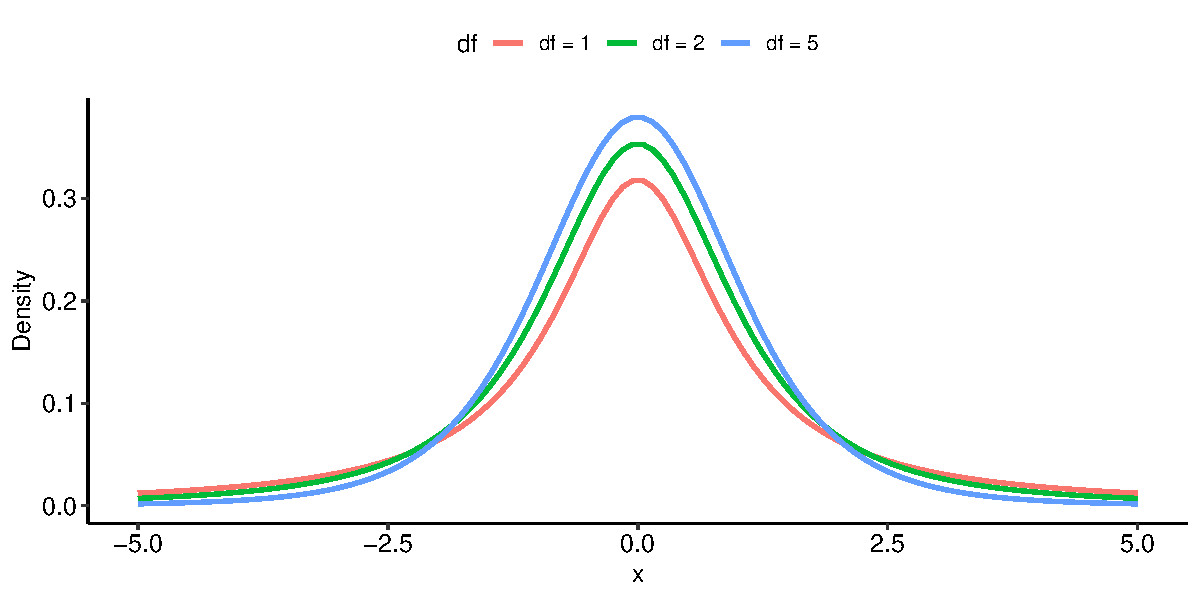
\includegraphics{_main_files/figure-latex/unnamed-chunk-131-1.pdf}

The one key difference between the t-distribution and the chi-square distribution from a mathematical point of view is that the t-distribution is symmetrical, much like the normal distribution (although they are not the same). Therefore, it is possible to get a negative t test statistic; however, this simply reflects the order in which the groups are being compared. E.g.

\begin{itemize}
\tightlist
\item
  Say that Group 1 - Group 2 gives a test statistic of t = 1.5.
\item
  If you were to enter the groups as Group 2 - Group 1 instead, the t would be -1.5. This simply reflects the ordering of the groups.
\end{itemize}

\subsection{The t-table}\label{the-t-table}

Once again, like the chi-square we have a beautiful little table for calculating a critical t-value. We won't go into too much depth over how this works because it works exactly like how it does for chi-squares - find the row corresponding to your degrees of freedom, then find the column corresponding to your alpha level.

Yes, there are a lot of cross-references to what we covered last week with chi-squares - and that's a good thing! The point here is that conceptually, the process of testing hypotheses using t-tests is exactly the same as what we did with chi-squares, but the specific design and maths are different.

\section{One-sample t-test}\label{one-sample-t-test}

The first test that we'll look at is the one-sample t-test, which is the most simple of the three that we will look at this week.

\subsection{One-sample t-test}\label{one-sample-t-test-1}

A one-sample t-test is used when we want to compare a sample against a hypothesised population value. It is useful when we already know the expected value of the parameter we're interested in, such as a population mean or a target value.

The basic hypotheses for a three-way interaction are:

\begin{itemize}
\tightlist
\item
  \(H_0\): The sample mean is not significantly different from the hypothesised mean. (i.e.~\(M = \mu\))
\item
  \(H_1\): The sample mean is significantly different from the hypothesised mean. (i.e.~\(M \neq \mu\))
\end{itemize}

It's worth noting that one-sample t-tests aren't that commonly used because they require you to know the population value (or, if you hypothesise a value, you need to justify why). However, they're included here because they're still a part of the t-test family, and they serve as a nice introduction to how t-tests work.

\subsection{Example data}\label{example-data}

Historically, scores in a fictional research methods class average at 72. This year, you are the subject coordinator for the first time, and you notice that last year's cohort appear to have really struggled. You want to see if there is a meaningful difference between the cohort's average grade and what the target grade should be.

Here's the dataset below:

\begin{Shaded}
\begin{Highlighting}[]
\NormalTok{w8\_grades }\OtherTok{\textless{}{-}} \FunctionTok{read\_csv}\NormalTok{(}\FunctionTok{here}\NormalTok{(}\StringTok{"data"}\NormalTok{, }\StringTok{"week\_8"}\NormalTok{, }\StringTok{"W8\_grades.csv"}\NormalTok{))}
\end{Highlighting}
\end{Shaded}

\begin{verbatim}
## Rows: 128 Columns: 2
## -- Column specification --------------------------------------------------------
## Delimiter: ","
## dbl (2): id, grade
## 
## i Use `spec()` to retrieve the full column specification for this data.
## i Specify the column types or set `show_col_types = FALSE` to quiet this message.
\end{verbatim}

\begin{Shaded}
\begin{Highlighting}[]
\FunctionTok{head}\NormalTok{(w8\_grades)}
\end{Highlighting}
\end{Shaded}

\begin{verbatim}
## # A tibble: 6 x 2
##      id grade
##   <dbl> <dbl>
## 1     1    60
## 2     2    66
## 3     3    70
## 4     4    72
## 5     5    63
## 6     6    71
\end{verbatim}

\subsection{Assumption checks}\label{assumption-checks}

There is only one relevant assumption that we need to check for the one-sample t-test: whether our data is distributed normally or not. We can do this in two ways. The first and quickest is through a test called the Shapiro-Wilks test (often abbreviated as the SW test). The SW test is a significant test of departures from normality. The statistic in question, W, is an index of normality. If W is close to 1, then data is normally distributed; the smaller W becomes, the more non-normal the data is.

A significant p-value on the SW test suggests that the data is non-normal. Thankfully, that isn't an issue here.

\begin{Shaded}
\begin{Highlighting}[]
\FunctionTok{shapiro.test}\NormalTok{(w8\_grades}\SpecialCharTok{$}\NormalTok{grade)}
\end{Highlighting}
\end{Shaded}

\begin{verbatim}
## 
##  Shapiro-Wilk normality test
## 
## data:  w8_grades$grade
## W = 0.98652, p-value = 0.2395
\end{verbatim}

The second way is through a QQ plot (Quantile-Quantile) plot. Essentially, these plot where data should be (if the data are normally distributed) against where the data actually is. If the normality assumption is intact, most of the data should lie on or close to the straight line, like the left plot. Data that looks like the right, where the data curves away from the central line, is more likely to be non-normally distributed.

\includesvg{img/w8_qqplots.svg}

\subsection{Output}\label{output-2}

Here are our descriptive statistics. They alone might already tell us something is going on:

\begin{Shaded}
\begin{Highlighting}[]
\NormalTok{w8\_grades }\SpecialCharTok{\%\textgreater{}\%}
  \FunctionTok{summarise}\NormalTok{(}
    \AttributeTok{mean =} \FunctionTok{mean}\NormalTok{(grade, }\AttributeTok{na.rm =} \ConstantTok{TRUE}\NormalTok{),}
    \AttributeTok{sd =} \FunctionTok{sd}\NormalTok{(grade, }\AttributeTok{na.rm =} \ConstantTok{TRUE}\NormalTok{),}
    \AttributeTok{median =} \FunctionTok{median}\NormalTok{(grade, }\AttributeTok{na.rm =} \ConstantTok{TRUE}\NormalTok{)}
\NormalTok{  ) }\SpecialCharTok{\%\textgreater{}\%}
\NormalTok{  knitr}\SpecialCharTok{::}\FunctionTok{kable}\NormalTok{(}\AttributeTok{digits =} \DecValTok{2}\NormalTok{)}
\end{Highlighting}
\end{Shaded}

\begin{tabular}{r|r|r}
\hline
mean & sd & median\\
\hline
67.09 & 5.38 & 67.5\\
\hline
\end{tabular}

To run a one-sample t-test, the basic function is the \texttt{t.test()} function. For a one-sample t-test, you must provide the argument \texttt{x} (the data) and \texttt{mu}, which is the hypothesised population mean.

Below is our output from the one-sample t-test. Our result tells us that there is a significant difference between the mean of the sample (\emph{M} = 67.09) and the hypothesised mean of 72 (\emph{p} \textless{} .001). The mean difference here is calculated as Sample - Hypothesis; therefore, a difference of -4.91 means that the sample mean is 4.91 units \emph{lower} than the population mean (which hopefully would have been evident from the descriptives anyway). This means that for some reason, last year's cohort are performing worse than the expected average.

R Note: Jamovi will give you a 95\% confidence interval around the mean difference as 95\% CI = {[}-5.85, -3.97{]}. R however will give you a CI around the actual \emph{mean}. In this case, the 95\% confidence interval for the group mean is {[}66.15, 68.03{]}. Really though, this is giving us the same information; 72 - 5.85 = 66.15, and 72 - 3.97 = 68.03. So the only difference is in what value is presented for the 95\% CI, but the actual inference itself doesn't change.

\begin{Shaded}
\begin{Highlighting}[]
\FunctionTok{t.test}\NormalTok{(w8\_grades}\SpecialCharTok{$}\NormalTok{grade, }\AttributeTok{mu =} \DecValTok{72}\NormalTok{)}
\end{Highlighting}
\end{Shaded}

\begin{verbatim}
## 
##  One Sample t-test
## 
## data:  w8_grades$grade
## t = -10.342, df = 127, p-value < 2.2e-16
## alternative hypothesis: true mean is not equal to 72
## 95 percent confidence interval:
##  66.14570 68.02617
## sample estimates:
## mean of x 
##  67.08594
\end{verbatim}

Anoter way of writing a one-sample t-test is to use \texttt{variable\ \textasciitilde{}\ 1} formula notation. The \texttt{\textasciitilde{}\ 1} is used to indicate that we are running a one-sample t-test. We still need to define \texttt{mu\ =\ 72} to set our hypothesised population mean.

\begin{Shaded}
\begin{Highlighting}[]
\FunctionTok{t.test}\NormalTok{(grade }\SpecialCharTok{\textasciitilde{}} \DecValTok{1}\NormalTok{, }\AttributeTok{data =}\NormalTok{ w8\_grades, }\AttributeTok{mu =} \DecValTok{72}\NormalTok{)}
\end{Highlighting}
\end{Shaded}

\begin{verbatim}
## 
##  One Sample t-test
## 
## data:  grade
## t = -10.342, df = 127, p-value < 2.2e-16
## alternative hypothesis: true mean is not equal to 72
## 95 percent confidence interval:
##  66.14570 68.02617
## sample estimates:
## mean of x 
##  67.08594
\end{verbatim}

Alternatively, you can use the \texttt{t\_test()} function in \texttt{rstatix}. This function also requires formula notation. \texttt{detailed\ =\ TRUE} will print a detailed output that will give the 95\% CI for the mean as well:

\begin{Shaded}
\begin{Highlighting}[]
\NormalTok{w8\_grades }\SpecialCharTok{\%\textgreater{}\%}
  \FunctionTok{t\_test}\NormalTok{(grade }\SpecialCharTok{\textasciitilde{}} \DecValTok{1}\NormalTok{, }\AttributeTok{mu =} \DecValTok{72}\NormalTok{, }\AttributeTok{detailed =} \ConstantTok{TRUE}\NormalTok{)}
\end{Highlighting}
\end{Shaded}

\begin{verbatim}
## # A tibble: 1 x 12
##   estimate .y.   group1 group2     n statistic        p    df conf.low conf.high
## *    <dbl> <chr> <chr>  <chr>  <int>     <dbl>    <dbl> <dbl>    <dbl>     <dbl>
## 1     67.1 grade 1      null ~   128     -10.3 1.47e-18   127     66.1      68.0
## # i 2 more variables: method <chr>, alternative <chr>
\end{verbatim}

\section{Independent samples t-test}\label{independent-samples-t-test}

The independent-samples t-test is one of the most common tests that you will see in literature - it is one of the bread-and-butter tests of many music psychologists (for better or worse).

\subsection{Independent samples}\label{independent-samples}

Independent samples t-tests are used when we want to compare two separate groups on one continuous outcome. They're therefore well-suited for data with one categorical IV with two levels, against one continuous outcome.

\subsection{Example data}\label{example-data-1}

For this example we'll use a contrived but really simple example. A group of self-reported professional and amateur musicians were asked how many years of training they had on their primary instrument.

\begin{Shaded}
\begin{Highlighting}[]
\NormalTok{w8\_training }\OtherTok{\textless{}{-}} \FunctionTok{read\_csv}\NormalTok{(}\FunctionTok{here}\NormalTok{(}\StringTok{"data"}\NormalTok{, }\StringTok{"week\_8"}\NormalTok{, }\StringTok{"W8\_training.csv"}\NormalTok{))}
\end{Highlighting}
\end{Shaded}

\begin{verbatim}
## Rows: 60 Columns: 3
## -- Column specification --------------------------------------------------------
## Delimiter: ","
## chr (1): Group
## dbl (2): Participant, Years_training
## 
## i Use `spec()` to retrieve the full column specification for this data.
## i Specify the column types or set `show_col_types = FALSE` to quiet this message.
\end{verbatim}

\begin{Shaded}
\begin{Highlighting}[]
\FunctionTok{head}\NormalTok{(w8\_training)}
\end{Highlighting}
\end{Shaded}

\begin{verbatim}
## # A tibble: 6 x 3
##   Participant Years_training Group       
##         <dbl>          <dbl> <chr>       
## 1           1              8 Professional
## 2           2              9 Professional
## 3           3              4 Professional
## 4           4              7 Professional
## 5           5              9 Professional
## 6           6              6 Professional
\end{verbatim}

Let us start with a nice plot:

\begin{Shaded}
\begin{Highlighting}[]
\NormalTok{w8\_training }\SpecialCharTok{\%\textgreater{}\%}
  \FunctionTok{group\_by}\NormalTok{(Group) }\SpecialCharTok{\%\textgreater{}\%}
  \FunctionTok{summarise}\NormalTok{(}
    \AttributeTok{mean =} \FunctionTok{mean}\NormalTok{(Years\_training, }\AttributeTok{na.rm =} \ConstantTok{TRUE}\NormalTok{),}
    \AttributeTok{sd =} \FunctionTok{sd}\NormalTok{(Years\_training, }\AttributeTok{na.rm =} \ConstantTok{TRUE}\NormalTok{),}
    \AttributeTok{se =}\NormalTok{ sd}\SpecialCharTok{/}\FunctionTok{n}\NormalTok{()}
\NormalTok{  ) }\SpecialCharTok{\%\textgreater{}\%}
  \FunctionTok{ggplot}\NormalTok{(}
    \FunctionTok{aes}\NormalTok{(}\AttributeTok{x =}\NormalTok{ Group, }\AttributeTok{y =}\NormalTok{ mean)}
\NormalTok{  ) }\SpecialCharTok{+}
  \FunctionTok{geom\_point}\NormalTok{(}\AttributeTok{size =} \DecValTok{3}\NormalTok{) }\SpecialCharTok{+}
  \FunctionTok{geom\_errorbar}\NormalTok{(}\FunctionTok{aes}\NormalTok{(}
    \AttributeTok{ymin =}\NormalTok{ mean }\SpecialCharTok{{-}} \FloatTok{1.96}\SpecialCharTok{*}\NormalTok{se,}
    \AttributeTok{ymax =}\NormalTok{ mean }\SpecialCharTok{+} \FloatTok{1.96}\SpecialCharTok{*}\NormalTok{se}
\NormalTok{  ), }\AttributeTok{width =} \FloatTok{0.2}\NormalTok{) }\SpecialCharTok{+}
  \FunctionTok{theme\_pubr}\NormalTok{()}
\end{Highlighting}
\end{Shaded}

\begin{center}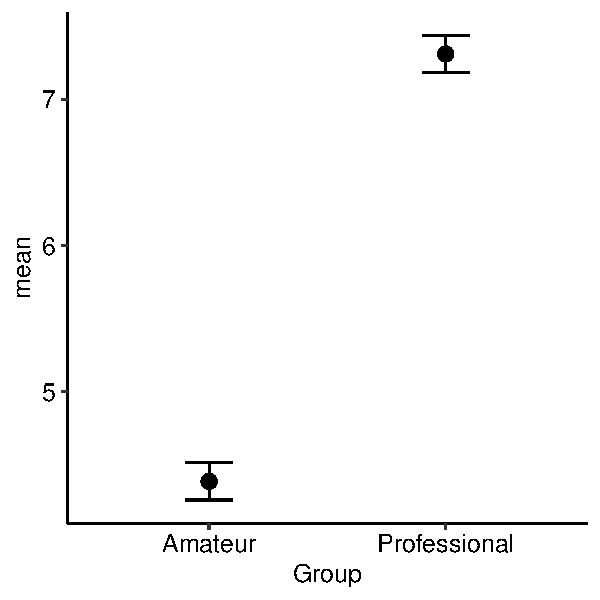
\includegraphics{_main_files/figure-latex/unnamed-chunk-140-1} \end{center}

\subsection{Assumption checks}\label{assumption-checks-1}

There are three main assumptions for a basic independent samples t-test:

\begin{itemize}
\tightlist
\item
  Data must be independent of each other - in other words, one person's response should not be influenced by another. This should come as a feature of good experimental design.
\item
  The equality of variance (homoscedasticity) assumption. The classical t-test assumes that each group has the same variance (homoscedasticity). We can test this using a significant test called Levene's test. If the test is significant (\emph{p} \textless{} .05), the assumption is violated. In our data, this assumption seems to be intact (\emph{F}(1, 58) = .114, \emph{p} = .737).
\end{itemize}

\begin{Shaded}
\begin{Highlighting}[]
\NormalTok{w8\_training }\SpecialCharTok{\%\textgreater{}\%}
  \FunctionTok{levene\_test}\NormalTok{(Years\_training }\SpecialCharTok{\textasciitilde{}}\NormalTok{ Group, }\AttributeTok{center =} \StringTok{"mean"}\NormalTok{)}
\end{Highlighting}
\end{Shaded}

\begin{verbatim}
## Warning in leveneTest.default(y = y, group = group, ...): group coerced to
## factor.
\end{verbatim}

\begin{verbatim}
## # A tibble: 1 x 4
##     df1   df2 statistic     p
##   <int> <int>     <dbl> <dbl>
## 1     1    58     0.114 0.737
\end{verbatim}

\begin{itemize}
\tightlist
\item
  The residuals should be normally distributed. This essentially has implications for how well the data behaves. We can test this in two ways. The first is using a normality test, like the Shapiro-Wilks (SW) test. Like Levene's test, if the result of this test is significant it suggests that the normality assumption is violated. In our data, this appears to be the case (\emph{W} = .946, \emph{p} = .011).
\end{itemize}

\begin{Shaded}
\begin{Highlighting}[]
\FunctionTok{shapiro.test}\NormalTok{(w8\_training}\SpecialCharTok{$}\NormalTok{Years\_training)}
\end{Highlighting}
\end{Shaded}

\begin{verbatim}
## 
##  Shapiro-Wilk normality test
## 
## data:  w8_training$Years_training
## W = 0.94685, p-value = 0.0111
\end{verbatim}

\subsection{Output}\label{output-3}

In reality, it's rare that any of these assumptions are fully met even when tests say they are (the tests we just mentioned can be biased). This is especially true for classical t-tests, which are very sensitive to violations. A consistently better alternative is to use the Welch t-test, which assumes the equality of variance assumption is not met. Welch t-tests are also fairly robust against the normality assumption, and so are more flexible without sacrificing accuracy.

Here's our output from R. Note that this is from a Welch t-test - R will do this by default.

\begin{Shaded}
\begin{Highlighting}[]
\FunctionTok{t.test}\NormalTok{(Years\_training }\SpecialCharTok{\textasciitilde{}}\NormalTok{ Group, }\AttributeTok{data =}\NormalTok{ w8\_training)}
\end{Highlighting}
\end{Shaded}

\begin{verbatim}
## 
##  Welch Two Sample t-test
## 
## data:  Years_training by Group
## t = -5.8586, df = 57.989, p-value = 2.33e-07
## alternative hypothesis: true difference in means between group Amateur and group Professional is not equal to 0
## 95 percent confidence interval:
##  -3.922048 -1.924448
## sample estimates:
##      mean in group Amateur mean in group Professional 
##                   4.387097                   7.310345
\end{verbatim}

\begin{Shaded}
\begin{Highlighting}[]
\NormalTok{w8\_training }\SpecialCharTok{\%\textgreater{}\%}
  \FunctionTok{t\_test}\NormalTok{(Years\_training }\SpecialCharTok{\textasciitilde{}}\NormalTok{ Group, }\AttributeTok{detailed =} \ConstantTok{TRUE}\NormalTok{)}
\end{Highlighting}
\end{Shaded}

\begin{verbatim}
## # A tibble: 1 x 15
##   estimate estimate1 estimate2 .y.   group1 group2    n1    n2 statistic       p
## *    <dbl>     <dbl>     <dbl> <chr> <chr>  <chr>  <int> <int>     <dbl>   <dbl>
## 1    -2.92      4.39      7.31 Year~ Amate~ Profe~    31    29     -5.86 2.33e-7
## # i 5 more variables: df <dbl>, conf.low <dbl>, conf.high <dbl>, method <chr>,
## #   alternative <chr>
\end{verbatim}

From this, we can see that the two groups do significantly differ on years of training (\emph{t}(57.99) = 5.86, \emph{p} \textless{} .001). We can use the mean difference value to see, well\ldots{} the difference in means between the two groups. In this case, professionals have 2.92 more years of training (on average; 95\% CI = {[}1.92, 3.92{]}) compared to amateurs.

(n.b.~the signs for t and the mean difference don't overly matter so long as they are interpreted in the right way. The output above calculates amateurs - professionals, which is why the values for both are negative; but if you were to force the test to run the other way round, the values would be the same with the signs flipped. Hence why descriptives and graphs are super important too!

If for some reason you do want R to run a Student's \emph{t}-test, you need to specify \texttt{var.equal\ =\ TRUE}. This tells R that we assume equality of variances.

\begin{Shaded}
\begin{Highlighting}[]
\FunctionTok{t.test}\NormalTok{(Years\_training }\SpecialCharTok{\textasciitilde{}}\NormalTok{ Group, }\AttributeTok{data =}\NormalTok{ w8\_training, }\AttributeTok{var.equal =} \ConstantTok{TRUE}\NormalTok{)}
\end{Highlighting}
\end{Shaded}

\begin{verbatim}
## 
##  Two Sample t-test
## 
## data:  Years_training by Group
## t = -5.8424, df = 58, p-value = 2.476e-07
## alternative hypothesis: true difference in means between group Amateur and group Professional is not equal to 0
## 95 percent confidence interval:
##  -3.924805 -1.921691
## sample estimates:
##      mean in group Amateur mean in group Professional 
##                   4.387097                   7.310345
\end{verbatim}

\begin{Shaded}
\begin{Highlighting}[]
\NormalTok{w8\_training }\SpecialCharTok{\%\textgreater{}\%}
  \FunctionTok{t\_test}\NormalTok{(Years\_training }\SpecialCharTok{\textasciitilde{}}\NormalTok{ Group, }\AttributeTok{detailed =} \ConstantTok{TRUE}\NormalTok{, }\AttributeTok{var.equal =} \ConstantTok{TRUE}\NormalTok{)}
\end{Highlighting}
\end{Shaded}

\begin{verbatim}
## # A tibble: 1 x 15
##   estimate estimate1 estimate2 .y.   group1 group2    n1    n2 statistic       p
## *    <dbl>     <dbl>     <dbl> <chr> <chr>  <chr>  <int> <int>     <dbl>   <dbl>
## 1    -2.92      4.39      7.31 Year~ Amate~ Profe~    31    29     -5.84 2.48e-7
## # i 5 more variables: df <dbl>, conf.low <dbl>, conf.high <dbl>, method <chr>,
## #   alternative <chr>
\end{verbatim}

\section{Paired-samples t-test}\label{paired-samples-t-test}

Here's our last test for the module, and it is again another bread-and-butter statistical test in literature: the paired-samples t-test.

\subsection{Paired-samples}\label{paired-samples}

Paired samples t-tests, as the name sort of implies, are used when we have a sample and we take measurements twice. Often, paired-samples t-tests are interested in testing the effect of time on an outcome; for example, a before-after design lends itself quite nicely to paired-samples and other repeated-measures tests.

The core hypotheses are very much the same here, aside from the caveat that the means are between conditions and not groups.

Mathematically, the paired-samples t-test is actually just a variant of the one-sample t-test. If we did a one-sample t-test on the differences between the two timepoints/conditions, we would get the same results. You can see a demonstration of this in the dropdown at the end of this section.

\subsection{Example data}\label{example-data-2}

For this example, we'll take a look at a simple interventions study. Participants were asked to answer a short list of questions relating to how they were feeling, once before an intervention and once afterwards. Higher scores represent better emotional states. The intervention was a series of self-regulation classes and exercises that the participants took twice a week. We're interested in seeing whether the intervention was effective.

\begin{Shaded}
\begin{Highlighting}[]
\NormalTok{w8\_symptoms }\OtherTok{\textless{}{-}} \FunctionTok{read\_csv}\NormalTok{(}\FunctionTok{here}\NormalTok{(}\StringTok{"data"}\NormalTok{, }\StringTok{"week\_8"}\NormalTok{, }\StringTok{"W8\_symptoms.csv"}\NormalTok{))}
\end{Highlighting}
\end{Shaded}

\begin{verbatim}
## Rows: 32 Columns: 2
## -- Column specification --------------------------------------------------------
## Delimiter: ","
## dbl (2): before, after
## 
## i Use `spec()` to retrieve the full column specification for this data.
## i Specify the column types or set `show_col_types = FALSE` to quiet this message.
\end{verbatim}

\begin{Shaded}
\begin{Highlighting}[]
\FunctionTok{head}\NormalTok{(w8\_symptoms)}
\end{Highlighting}
\end{Shaded}

\begin{verbatim}
## # A tibble: 6 x 2
##   before after
##    <dbl> <dbl>
## 1     14    18
## 2     18    17
## 3     14    18
## 4     10    18
## 5     14    12
## 6     14    13
\end{verbatim}

R-note: Data for paired-samples \emph{t}-tests can either be in wide form or long form, and this depends on the specific function used. Our dataset is already in wide form as we have one column for before and one for after, so the following code will create a long-form version:

\begin{Shaded}
\begin{Highlighting}[]
\CommentTok{\# Pivot to long format}
\NormalTok{w8\_symptoms\_long }\OtherTok{\textless{}{-}}\NormalTok{ w8\_symptoms }\SpecialCharTok{\%\textgreater{}\%}
  \FunctionTok{pivot\_longer}\NormalTok{(}
    \AttributeTok{cols =} \FunctionTok{everything}\NormalTok{(),}
    \AttributeTok{names\_to =} \StringTok{"time"}\NormalTok{,}
    \AttributeTok{values\_to =} \StringTok{"symptom\_score"}
\NormalTok{  )}

\CommentTok{\# Display start of new data}
\FunctionTok{head}\NormalTok{(w8\_symptoms\_long)}
\end{Highlighting}
\end{Shaded}

\begin{verbatim}
## # A tibble: 6 x 2
##   time   symptom_score
##   <chr>          <dbl>
## 1 before            14
## 2 after             18
## 3 before            18
## 4 after             17
## 5 before            14
## 6 after             18
\end{verbatim}

\subsection{Assumption checks}\label{assumption-checks-2}

Similar to other tests, we need to check normality. Here, the assumption is whether the differences between time 1 and 2 are normally distributed (not necessarily time 1 and 2 themselves). Hence, when we run a Shapiro-Wilks test we're running this on the values we get from Time 1 - Time 2.

In our data, this assumption seems to be intact (\emph{W} .985, \emph{p} = .918).

\begin{Shaded}
\begin{Highlighting}[]
\FunctionTok{shapiro.test}\NormalTok{(w8\_symptoms}\SpecialCharTok{$}\NormalTok{before }\SpecialCharTok{{-}}\NormalTok{ w8\_symptoms}\SpecialCharTok{$}\NormalTok{after)}
\end{Highlighting}
\end{Shaded}

\begin{verbatim}
## 
##  Shapiro-Wilk normality test
## 
## data:  w8_symptoms$before - w8_symptoms$after
## W = 0.98465, p-value = 0.9177
\end{verbatim}

\subsection{Output}\label{output-4}

In R, you can do pairwise t-tests using the default \texttt{t.test()} (or the \texttt{rstatix} equivalent \texttt{t\_test()}) function. In both methods, you must set \texttt{paired\ =\ TRUE} in order to run a paired t-test. However, there is one key difference: the base \texttt{t.test()} requires data in \emph{wide} format, whereas \texttt{rstatix::t\_test()} requires data in \emph{long} format. Here are both methods.

For the base \texttt{t.test()} function, your data needs to be in wide format. From there it is as simple as giving the two columns as the arguments to the function, and setting \texttt{paired\ =\ TRUE}:

\begin{Shaded}
\begin{Highlighting}[]
\FunctionTok{t.test}\NormalTok{(}\AttributeTok{x =}\NormalTok{ w8\_symptoms}\SpecialCharTok{$}\NormalTok{before, }\AttributeTok{y =}\NormalTok{ w8\_symptoms}\SpecialCharTok{$}\NormalTok{after, }\AttributeTok{paired =} \ConstantTok{TRUE}\NormalTok{)}
\end{Highlighting}
\end{Shaded}

\begin{verbatim}
## 
##  Paired t-test
## 
## data:  w8_symptoms$before and w8_symptoms$after
## t = -2.9501, df = 31, p-value = 0.005999
## alternative hypothesis: true mean difference is not equal to 0
## 95 percent confidence interval:
##  -4.651185 -0.848815
## sample estimates:
## mean difference 
##           -2.75
\end{verbatim}

Alternatively, you can use the below notation. \texttt{Pair(before,\ after)} indicates that we want R to treat the \texttt{before} and \texttt{after} variables as paired data. The \texttt{\textasciitilde{}\ 1}, as we saw before, indicates that this is a one-sample t-test. This is because a paired-samples t-test is functionally equivalent to a one-sample t-test on the differences between conditions (see the expandable dropdown below for more details).

\begin{Shaded}
\begin{Highlighting}[]
\FunctionTok{t.test}\NormalTok{(}\FunctionTok{Pair}\NormalTok{(before, after) }\SpecialCharTok{\textasciitilde{}} \DecValTok{1}\NormalTok{, }\AttributeTok{data =}\NormalTok{ w8\_symptoms)}
\end{Highlighting}
\end{Shaded}

\begin{verbatim}
## 
##  Paired t-test
## 
## data:  Pair(before, after)
## t = -2.9501, df = 31, p-value = 0.005999
## alternative hypothesis: true mean difference is not equal to 0
## 95 percent confidence interval:
##  -4.651185 -0.848815
## sample estimates:
## mean difference 
##           -2.75
\end{verbatim}

If you prefer rstatix, on the other hand, your data needs to be in long format. After that, you can pass the test as a formula much like how you would do so in the indendent samples case:

\begin{Shaded}
\begin{Highlighting}[]
\NormalTok{w8\_symptoms\_long }\SpecialCharTok{\%\textgreater{}\%}
  \FunctionTok{t\_test}\NormalTok{(symptom\_score }\SpecialCharTok{\textasciitilde{}}\NormalTok{ time, }\AttributeTok{paired =} \ConstantTok{TRUE}\NormalTok{, }\AttributeTok{detailed =} \ConstantTok{TRUE}\NormalTok{)}
\end{Highlighting}
\end{Shaded}

\begin{verbatim}
## # A tibble: 1 x 13
##   estimate .y.          group1 group2    n1    n2 statistic     p    df conf.low
## *    <dbl> <chr>        <chr>  <chr>  <int> <int>     <dbl> <dbl> <dbl>    <dbl>
## 1     2.75 symptom_sco~ after  before    32    32      2.95 0.006    31    0.849
## # i 3 more variables: conf.high <dbl>, method <chr>, alternative <chr>
\end{verbatim}

The mean symptom scores of the two timepoints are significantly different (\emph{t}(31) = 2.95, \emph{p} = .006). Based on the means and mean difference (2.75; 95\% CI = {[}0.85, 4.65{]}), participants reported having significantly better emotional states after the intervention compared to beforehand.

Paired samples using the one-sample t-test

Mathematically, all a paired-samples t-test is doing is running a one-sample t-test on the differences between the two timepoints/groups, Below is a demonstration of how paired-samples tests can be run using the one-sample t-test.

Let's start by returning to the wide version of our dataset. We first need to calculate the difference between the \texttt{before} and \texttt{after} columns, which we can easily do with \texttt{mutate()}.

\begin{Shaded}
\begin{Highlighting}[]
\NormalTok{w8\_symptoms }\OtherTok{\textless{}{-}}\NormalTok{ w8\_symptoms }\SpecialCharTok{\%\textgreater{}\%}
  \FunctionTok{mutate}\NormalTok{(}
    \AttributeTok{diff =}\NormalTok{ before }\SpecialCharTok{{-}}\NormalTok{ after}
\NormalTok{  )}

\NormalTok{w8\_symptoms}
\end{Highlighting}
\end{Shaded}

\begin{verbatim}
## # A tibble: 32 x 3
##    before after  diff
##     <dbl> <dbl> <dbl>
##  1     14    18    -4
##  2     18    17     1
##  3     14    18    -4
##  4     10    18    -8
##  5     14    12     2
##  6     14    13     1
##  7     11    20    -9
##  8     12    18    -6
##  9     15    18    -3
## 10     18     8    10
## # i 22 more rows
\end{verbatim}

We can run a one-sample t-test on the differences now, with the null hypothesis value being 0 - i.e.~we are testing the null hypothesis that the mean differences are not significantly different from 0.

\begin{Shaded}
\begin{Highlighting}[]
\FunctionTok{t.test}\NormalTok{(w8\_symptoms}\SpecialCharTok{$}\NormalTok{diff }\SpecialCharTok{\textasciitilde{}} \DecValTok{1}\NormalTok{, }\AttributeTok{mu =} \DecValTok{0}\NormalTok{)}
\end{Highlighting}
\end{Shaded}

\begin{verbatim}
## 
##  One Sample t-test
## 
## data:  w8_symptoms$diff
## t = -2.9501, df = 31, p-value = 0.005999
## alternative hypothesis: true mean is not equal to 0
## 95 percent confidence interval:
##  -4.651185 -0.848815
## sample estimates:
## mean of x 
##     -2.75
\end{verbatim}

As we can see, the results are equivalent to the output of the paired-samples t-test above. Note too that our Shapiro-Wilks test will also give equivalent results if it is run on the differences directly.

\section{Cohen's d}\label{cohens-d}

This might be starting to sound a little familiar by now, but here are some effect sizes for t-tests. Note that they're different to the Cramer's V we saw in the chi-square test of independence last week - this is because it is a) conceptually different and b) interpreted differently too.

\subsection{\texorpdfstring{What is Cohen's \emph{d}?}{What is Cohen's d?}}\label{what-is-cohens-d}

Cohen's d is a measure of effect size that is used when comparing between two means (i.e.~in a t-test). It essentially is a measure of the distance between the two means. See below for three pairs of means:

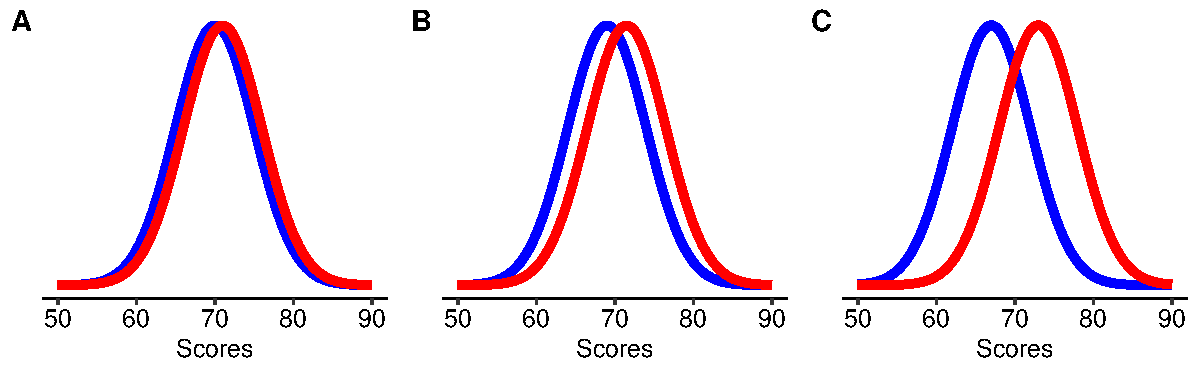
\includegraphics{_main_files/figure-latex/unnamed-chunk-153-1.pdf}

If two groups aren't all that different (e.g.~panel A), then any effect of group will be small or negligible. If the two groups are further apart, however (like panel C), there is a more obvious effect of group - and so the size of the effect itself will be larger. Cohen's \emph{d} essentially is a measure of this `distance'.

The basic formula for calculating Cohen's d is:
\[
d = \frac{M_1 - M_2}{\sigma_{pooled}}
\]

In other words, Cohen's \emph{d} is calculated by taking the difference between the two group means and dividing that by the pooled standard deviation across both groups. Pooled SD is essentially an aggregate SD across both groups in the sample, and not something we'll concern ourselves with this week (because like the maths for the t-statistic, the calculation of the pooled SD depends on the test and is hard).

\subsection{\texorpdfstring{Interpreting Cohen's \emph{d}}{Interpreting Cohen's d}}\label{interpreting-cohens-d}

Cohen provided some now-famous guidelines for interpreting the size of Cohen's d values:

\begin{tabular}{l|l}
\hline
Effect size & Interpretation\\
\hline
d = .20 & Small\\
\hline
d = .50 & Medium\\
\hline
d = .80 & Large\\
\hline
\end{tabular}

\subsection{\texorpdfstring{Calculating Cohen's \emph{d} in R}{Calculating Cohen's d in R}}\label{calculating-cohens-d-in-r}

The \texttt{cohens\_d()} function from \texttt{effectsize} can handle the calculation of effect sizes for all three variants of t-tests. One thing that's quite nice about this function is that the required syntax for \texttt{cohens\_d()} is nearly identical to that for \texttt{t.test()} - meaning that the correct type of Cohen's \emph{d} (one-sample, independent samples, paired) will be calculated based on what you put in.

For a one-sample t-test, for instance, you can write the syntax exactly as you would for \texttt{t.test()}:

\begin{Shaded}
\begin{Highlighting}[]
\CommentTok{\# One{-}sample}
\CommentTok{\# t.test(w8\_grades$grade, mu = 72)}
\NormalTok{effectsize}\SpecialCharTok{::}\FunctionTok{cohens\_d}\NormalTok{(w8\_grades}\SpecialCharTok{$}\NormalTok{grade, }\AttributeTok{mu =} \DecValTok{72}\NormalTok{)}
\end{Highlighting}
\end{Shaded}

\begin{verbatim}
## Cohen's d |         95% CI
## --------------------------
## -0.91     | [-1.12, -0.71]
## 
## - Deviation from a difference of 72.
\end{verbatim}

The alternate way of specifying a one-sample t-test, the \texttt{var\ \textasciitilde{}\ 1} format, also works. \texttt{cohens\_d()} will recognise both.

\begin{Shaded}
\begin{Highlighting}[]
\CommentTok{\# One{-}sample {-} alternate}
\CommentTok{\# t.test(grade \textasciitilde{} 1, data = w8\_grades, mu = 72)}
\NormalTok{effectsize}\SpecialCharTok{::}\FunctionTok{cohens\_d}\NormalTok{(grade }\SpecialCharTok{\textasciitilde{}} \DecValTok{1}\NormalTok{, }\AttributeTok{data =}\NormalTok{ w8\_grades, }\AttributeTok{mu =} \DecValTok{72}\NormalTok{)}
\end{Highlighting}
\end{Shaded}

\begin{verbatim}
## Cohen's d |         95% CI
## --------------------------
## -0.91     | [-1.12, -0.71]
## 
## - Deviation from a difference of 72.
\end{verbatim}

For an independent samples t-test, you can give it \emph{almost} the same. The only change is that by default, \texttt{cohens\_d()} will calculate Cohen's \emph{d} assuming equal variance. In order for our value of \emph{d} to match a Welch-samples t-test, we need to set \texttt{pooled\_sd\ =\ FALSE} (which makes the syntax slightly different to \texttt{t.test()}).

\begin{Shaded}
\begin{Highlighting}[]
\CommentTok{\# Independent samples}
\CommentTok{\# t.test(Years\_training \textasciitilde{} Group, data = w8\_training)}
\NormalTok{effectsize}\SpecialCharTok{::}\FunctionTok{cohens\_d}\NormalTok{(Years\_training }\SpecialCharTok{\textasciitilde{}}\NormalTok{ Group, }\AttributeTok{data =}\NormalTok{ w8\_training, }\AttributeTok{pooled\_sd =} \ConstantTok{FALSE}\NormalTok{)}
\end{Highlighting}
\end{Shaded}

\begin{verbatim}
## Cohen's d |         95% CI
## --------------------------
## -1.51     | [-2.08, -0.93]
## 
## - Estimated using un-pooled SD.
\end{verbatim}

Finally, for a paired-samples t-test the developers of \texttt{effectsize} recommend using the \texttt{rm\_d()} function, which stands for repeated-measures Cohen's \emph{d}. This function takes the same basic syntax as \texttt{t.test()} for paired-samples t-tests, including the use of wide data, but a couple of extra arguments are required.

\begin{itemize}
\tightlist
\item
  \texttt{method\ =\ "z"} defines how the pooled SD term is calculated. There are six possible options, but this option gives the standard calculation.
\item
  \texttt{adjust\ =\ FALSE}: calculates Hedges' G, which is an alternative effect size that corrects for small sample bias. We won't worry about this here, so we will set this to \texttt{FALSE}.
\end{itemize}

Note that like the other functions, you can either provide the arguments in \texttt{Pairs()\ \textasciitilde{}\ 1} or by subsetting the columns (\texttt{x\ =\ x\$1,\ y\ =\ x\$2}).

\begin{Shaded}
\begin{Highlighting}[]
\CommentTok{\# Paired sample {-} works with wide data}
\CommentTok{\# t.test(Pair(before, after) \textasciitilde{} 1, data = w8\_symptoms)}
\NormalTok{effectsize}\SpecialCharTok{::}\FunctionTok{rm\_d}\NormalTok{(}\FunctionTok{Pair}\NormalTok{(before, after) }\SpecialCharTok{\textasciitilde{}} \DecValTok{1}\NormalTok{, }\AttributeTok{data =}\NormalTok{ w8\_symptoms, }\AttributeTok{method =} \StringTok{"z"}\NormalTok{, }\AttributeTok{adjust =} \ConstantTok{FALSE}\NormalTok{)}
\end{Highlighting}
\end{Shaded}

\begin{verbatim}
## d (z) |         95% CI
## ----------------------
## -0.52 | [-0.89, -0.15]
\end{verbatim}

\begin{Shaded}
\begin{Highlighting}[]
\CommentTok{\# t.test(x = w8\_symptoms$before, y = w8\_symptoms$after, paired = TRUE)}
\NormalTok{effectsize}\SpecialCharTok{::}\FunctionTok{rm\_d}\NormalTok{(}\AttributeTok{x =}\NormalTok{ w8\_symptoms}\SpecialCharTok{$}\NormalTok{before, }\AttributeTok{y =}\NormalTok{ w8\_symptoms}\SpecialCharTok{$}\NormalTok{after, }\AttributeTok{method =} \StringTok{"z"}\NormalTok{, }\AttributeTok{adjust =} \ConstantTok{FALSE}\NormalTok{)}
\end{Highlighting}
\end{Shaded}

\begin{verbatim}
## d (z) |         95% CI
## ----------------------
## -0.52 | [-0.89, -0.15]
\end{verbatim}

\subsection{\texorpdfstring{Alternative using \texttt{rstatix}}{Alternative using rstatix}}\label{alternative-using-rstatix}

Alternatively, you can use the \texttt{rstatix} package. This will give the same values, but the confidence intervals generated by \texttt{effectsize} are traditional confidence intervals, whereas \texttt{rstaix} uses a different method (which we need not concern ourselves with). In any case, the actual width of the intervals should be similar. Just note that for paired samples Cohen's \emph{d}, long data is required (as is the case with t-tests in \texttt{rstatix}).

For a one-sample t-test, the formula once again needs to be in \texttt{var\ \textasciitilde{}\ 1} format and \texttt{mu} must be specified:

\begin{Shaded}
\begin{Highlighting}[]
\NormalTok{w8\_grades }\SpecialCharTok{\%\textgreater{}\%} 
\NormalTok{  rstatix}\SpecialCharTok{::}\FunctionTok{cohens\_d}\NormalTok{(grade }\SpecialCharTok{\textasciitilde{}} \DecValTok{1}\NormalTok{, }\AttributeTok{mu =} \DecValTok{72}\NormalTok{, }\AttributeTok{ci =} \ConstantTok{TRUE}\NormalTok{, }\AttributeTok{ci.type =} \StringTok{"norm"}\NormalTok{) }
\end{Highlighting}
\end{Shaded}

\begin{verbatim}
## # A tibble: 1 x 8
##   .y.   group1 group2     effsize     n conf.low conf.high magnitude
## * <chr> <chr>  <chr>        <dbl> <int>    <dbl>     <dbl> <ord>    
## 1 grade 1      null model  -0.914   128     -1.1     -0.71 large
\end{verbatim}

For an independent-samples t-test:

\begin{Shaded}
\begin{Highlighting}[]
\NormalTok{w8\_training }\SpecialCharTok{\%\textgreater{}\%}
\NormalTok{  rstatix}\SpecialCharTok{::}\FunctionTok{cohens\_d}\NormalTok{(Years\_training }\SpecialCharTok{\textasciitilde{}}\NormalTok{ Group, }\AttributeTok{ci =} \ConstantTok{TRUE}\NormalTok{, }\AttributeTok{ci.type =} \StringTok{"norm"}\NormalTok{)}
\end{Highlighting}
\end{Shaded}

\begin{verbatim}
## # A tibble: 1 x 9
##   .y.            group1  group2 effsize    n1    n2 conf.low conf.high magnitude
## * <chr>          <chr>   <chr>    <dbl> <int> <int>    <dbl>     <dbl> <ord>    
## 1 Years_training Amateur Profe~   -1.51    31    29    -2.07     -0.87 large
\end{verbatim}

For a paired-samples t-test, \texttt{paired\ =\ TRUE} must be selected:

\begin{Shaded}
\begin{Highlighting}[]
\NormalTok{w8\_symptoms\_long }\SpecialCharTok{\%\textgreater{}\%}
\NormalTok{  rstatix}\SpecialCharTok{::}\FunctionTok{cohens\_d}\NormalTok{(symptom\_score }\SpecialCharTok{\textasciitilde{}}\NormalTok{ time, }\AttributeTok{paired =} \ConstantTok{TRUE}\NormalTok{, }\AttributeTok{ci =} \ConstantTok{TRUE}\NormalTok{, }\AttributeTok{ci.type =} \StringTok{"norm"}\NormalTok{)}
\end{Highlighting}
\end{Shaded}

\begin{verbatim}
## # A tibble: 1 x 9
##   .y.           group1 group2 effsize    n1    n2 conf.low conf.high magnitude
## * <chr>         <chr>  <chr>    <dbl> <int> <int>    <dbl>     <dbl> <ord>    
## 1 symptom_score after  before   0.522    32    32     0.09       0.9 moderate
\end{verbatim}

The Canvas version asks you to interpret each of these effect sizes, but\ldots{} \texttt{rstatix} will automatically label this for you!

\chapter{ANOVAs}\label{anovas}

t-tests, as we saw last week, were a simple way of comparing a
continuous outcome between two groups or conditions (i.e.~one
categorical variable with two levels). However, it's also common to
compare across three or more groups when doing real research. To test
this kind of hypothesis where we have three or more groups, we need to
turn to a different method - the ANOVA. ANOVAs are useful when you have
one categorical IV with 3+ levels, and one continuous DV.

The ANOVA is perhaps one of the most common statistical tests you will
see in music psychology literature, in part because they generalise to a
lot of research designs. In many respects, this week is fairly important
in terms of knowing how to conduct an ANOVA and when. We'll only be
stepping through the basics this week, but there are some really
important fundamentals to cover here.

It's also common to analyse two independent variables against one
dependent variable. These too can be done using ANOVAs. While we won't
go into this in this module, there will be an Extension Module that
deals with this separately - check it out sometime around Week 10/11 if
you're interested.

By the end of this module you should be able to:

\begin{itemize}
\tightlist
\item
  Understand and describe the conceptual basis of an analysis of
  variance
\item
  Describe how an ANOVA is calculated
\item
  Conduct both one-way ANOVAs and one-way repeated ANOVAs, including
  their assumption tests
\item
  Interpret the output of the ANOVAs and report their findings
\end{itemize}

\begin{figure}

{\centering \includegraphics{https://imgs.xkcd.com/comics/third_way_2x} 

}

\caption{[xkcd: Third Way](https://xkcd.com/1285/)}\label{fig:unnamed-chunk-164}
\end{figure}

\section{Anovas and the F-distribution}\label{anovas-and-the-f-distribution}

Just as we've done so for chi-squares and t-tests, let's begin with an
overview of the mathematical and conceptual underpinnings of the ANOVA.

\subsection{The basic logic of ANOVAs}\label{the-basic-logic-of-anovas}

As we said in the introductory page, ANOVA stands for ANalysis Of VAriance. This essentially sums up how an ANOVA works in principle. ANOVAs can be used when analysing a categorical IV with two or more groups (typically 3+) and a continuous DV. As the setup suggests, ANOVAs are a good way of comparing different groups on a singular outcome.

The most basic hypotheses for an ANOVA center around whether or not the
means between groups are significantly different, i.e.:

\begin{itemize}
\tightlist
\item
  \(H_0\): The means between groups are not significantly different.
  (i.e.~\(\mu_1 = \mu_2 = ... \mu_k\))
\item
  \(H_1\): The means between groups are significantly different.
  (i.e.\(\mu_1 \neq \mu_2 \neq ... \mu_k\))
\end{itemize}

How do we test for this? The basic logic of the ANOVA is this: Whenever
we have data that we categorise into different groups, we end up with
two key sources of variability, or variance: variance that exists
between groups, and variance that exists within groups:

\includegraphics{_main_files/figure-latex/unnamed-chunk-165-1.pdf}

Pretend that the three curves above represent data covering three
different groups, and that we've hypothesised that there are three
different means. Collectively, this data has a certain amount of
variance.

The first fundamental to recognise is that this total variance can be
broken down into variance between groups and variance within groups:

\[
Variance_{total} = Variance_{between} + Variance_{within}
\]

The variability between the groups would simply be the variance between
the blue curve and the orange curve - in other words, how far apart the
two sets of data are (in a simplistic sense). The within-group variance,
on the other hand, is how much variance there is within each curve. If
there is a lot of within-group variance within each curve, that would
mean that (thinking back to Module 5) each group's curve would be spread
widely.

If you're following the logic of this so far, the consequences of high
within-group variance might be obvious - the two curves would
significantly overlap. In contrast, if the between-group variance is far
higher than the within-group variance, the curves may not overlap much
at all - suggesting that the means of the two groups really are
different.

This forms the basis of the ANOVA's F-test, which is a ratio of
variance:

\[
F = \frac{Variance_{between}}{Variance_{within}}
\]

We will see this more in practice on the next page, but the
\emph{F}-statistic, which we use as part of significance testing in ANOVAs, is
calculated by simply dividing the between-group variance by the
within-group variance.

\subsection{The F-distribution}\label{the-f-distribution}

Like the other tests we've encountered so far, ANOVAs have their own
underlying distribution. In this instance, this is the \emph{F} distribution,
which describes how the F-statistic behaves. We won't go far into the
maths around this, but the key here is that the F distribution is
characterised by two sets of degrees of freedom: one that relates to the
between-groups variance/effect, and one that relates to the
within-groups variance. One thing to note here is the terminology in the
headers of each graph: the first number in the brackets refers to the
between-groups variance, while the second number refers to the
within-groups variance.

\includegraphics{_main_files/figure-latex/unnamed-chunk-166-1.pdf}

\subsection{\texorpdfstring{\emph{F}-statistic tables}{F-statistic tables}}\label{f-statistic-tables}

And, once again, we have a special \emph{F}-table to determine critical \emph{F}
values, given two degrees of freedom values. However, given that we have
two degrees of freedom the process is a little bit more complicated.
Most \emph{F}-stat tables actually provide multiple tables, corresponding to
different alpha levels. For now, we will always use the table
corresponding to alpha = 0.05, a snippet of which is below:

\begin{Shaded}
\begin{Highlighting}[]
\NormalTok{knitr}\SpecialCharTok{::}\FunctionTok{include\_graphics}\NormalTok{(}\FunctionTok{here}\NormalTok{(}\StringTok{"img/w9\_f{-}table.png"}\NormalTok{))}
\end{Highlighting}
\end{Shaded}

\includegraphics{img/w9_f-table.png}

To read this table, you need to know both degrees of freedom (more on
how to find that on the next page). The columns, marked df1, refer to
the first df value (between-groups), while the rows correspond to the
second df value (within-groups).

So, for example, if we have an \emph{F}-test with degrees of freedom of (4,
10), we would first need to find the column that corresponds to 4 (our
df1), and then the row that corresponds to df2 = 10. Reading the cell at
the intersection would give us a critical \emph{F}-statistic of 3.48; this is
the value our \emph{F}-statistic would need to be greater than to be
significant at the p \textless{} .05 level.

\section{The ANOVA table}\label{the-anova-table}

Every time we do an ANOVA, there are actually a raft of calculations
that have to occur in order to get our test statistic and \emph{p}-value.
Statistical software will display all of this in the form of an ANOVA
table, which we cover below.

Don't stress too much about the maths here - while the quiz does include
one question about this, the question itself isn't difficult (and you
won't be expected to do any of this by hand otherwise). The reason why
we go through this, however, is to demonstrate the conceptual logic from
the previous page.

\subsection{The ANOVA table}\label{the-anova-table-1}

On the previous page, we talked in depth about how the \emph{F} statistic is
calculated, and what shapes the overall distribution. But how do we
actually calculate all of that stuff to begin with from raw data? Enter
the ANOVA table, a beautiful (remember, beauty is subjective) way of
calculating this information and laying it all out to see.

The basic ANOVA table looks like this, which you will see on any
statistical package you use.

\begin{longtable}[]{@{}
  >{\raggedright\arraybackslash}p{(\columnwidth - 10\tabcolsep) * \real{0.1667}}
  >{\raggedright\arraybackslash}p{(\columnwidth - 10\tabcolsep) * \real{0.1667}}
  >{\raggedright\arraybackslash}p{(\columnwidth - 10\tabcolsep) * \real{0.1667}}
  >{\raggedright\arraybackslash}p{(\columnwidth - 10\tabcolsep) * \real{0.1667}}
  >{\raggedright\arraybackslash}p{(\columnwidth - 10\tabcolsep) * \real{0.1667}}
  >{\raggedright\arraybackslash}p{(\columnwidth - 10\tabcolsep) * \real{0.1667}}@{}}
\toprule\noalign{}
\begin{minipage}[b]{\linewidth}\raggedright
\end{minipage} & \begin{minipage}[b]{\linewidth}\raggedright
Sums of squares (SS)
\end{minipage} & \begin{minipage}[b]{\linewidth}\raggedright
Degrees of freedom (df)
\end{minipage} & \begin{minipage}[b]{\linewidth}\raggedright
Mean square (MS)
\end{minipage} & \begin{minipage}[b]{\linewidth}\raggedright
F
\end{minipage} & \begin{minipage}[b]{\linewidth}\raggedright
\emph{p}
\end{minipage} \\
\midrule\noalign{}
\endhead
\bottomrule\noalign{}
\endlastfoot
Group (our effect) & & & & & \\
Error/Residual & & & & & \\
Total & & & & & \\
\end{longtable}

A couple of terminology-related things here.

\begin{itemize}
\tightlist
\item
  `Group' in this context is our independent variable (i.e.~the effect
  of group)- this is our between-subject variance.
\item
  `Error' or `Residual' is the within-group variance.
\end{itemize}

Let's use the below data to calculate this by hand.

\begin{tabular}{l|l|l}
\hline
Group 1 & Group 2 & Group 3\\
\hline
1 & 2 & 5\\
\hline
2 & 4 & 8\\
\hline
3 & 5 & 6\\
\hline
2 & 3 & 7\\
\hline
Mean: 2 & Mean: 3.5 & Mean: 6\\
\hline
\end{tabular}

The grand mean (i.e.~the mean across all 12 pieces of data) is 4. Keep
this in mind.

Time to strap in - there are a lot of formulae involved!

\subsection{Sums of squares}\label{sums-of-squares}

The sum of squares quantifies how far each observation is from the
average - just like how it is calculated in the formula for standard
deviations. For an ANOVA, we have two sets of SS to calculate - one for
the between-groups term, and one for the within-groups/error.

\textbf{Between}

The formula for the between-groups sum of squares (\(SS_b\)) is:

\[
SS_b = \Sigma n(\bar x - \bar X)^2
\]

In words, this means:

\begin{itemize}
\tightlist
\item
  Take each group's mean (\(\bar x\)), and subtract them from the grand
  mean (\(\bar X\))
\item
  Square that difference
\item
  Multiply it by n, the size of each group
\item
  Add them all up.
\end{itemize}

Let's do that for our fictional data. Our group means are Group 1 = 2,
Group 2 = 3.5 and Group 3 = 6.5.
\(SS_b = 4(2-4)^2 + 4(3.5-4)^2 + 4(6.5-4)^2\)
\(SS_b = (4 \times 4) + (4 \times 0.25) + (4 \times 6.25)\) \(SS_b = 42\)

\textbf{Within}

For the within-group sum of squares, the formula is:

\[
SS_w = \Sigma (x - \bar x)^2
\]

This one is a bit more tedious. It means:

\begin{itemize}
\tightlist
\item
  Take each observation (\(x\)), and subtract them from their group mean
  (\(\bar x\))
\item
  Square that difference
\item
  Add them all up.
\end{itemize}

So for our data, it would look something like..
\[
SS_w = (1-2)^2 + (2-2)^2 + (3-2)^2 + (2-2)^2 + (2-3.5)^2 + (4-3.5)^2 + (5-3.5)^2 + (3-3.5)^2 + (5-6.5)^2 + (8-6.5)^2 + (6-6.5)^2 + (7-6.5)^2
\]
\[SS_w = 12\].

\subsection{Degrees of freedom}\label{degrees-of-freedom}

Because we have a term for between-groups and within-groups effects, we
also have degrees of freedom for both (think back to the previous page).
Thankfully, unlike the mess above the formulae here are relatively
simple.

\textbf{Between}

The between-groups df is given as:

\[
df_b = k - 1
\]

Where k = the number of groups. So, in our data, \(df_b = 3 -1 = 2\) (as
we have 3 groups).

\textbf{Within}

The within-groups df is given as:

\[
df_b = N - k
\]

Where k = the number of groups, and \emph{N} is the total sample size (in our
case, 12). So \(df_w = 12 -3 = 9\) (as we have 3 groups and 12 data points
in total).

\subsection{Mean squares}\label{mean-squares}

The mean squares is another value for variance that essentially
standardises the sum of squares by the degrees of freedom. The formula
for MS between and within is the same:

\[
MS = \frac{SS}{df}
\]

We've calculated SS and df for both our between and within-groups
effects, so we can substitute these values in to calculate a mean square
value for both:

\[MS_b = \frac{SS_b}{df_b}\]
\[MS_w = \frac{SS_w}{df_w}\]

Putting in our values that we calculated earlier, we get:

\[MS_b = \frac{42}{2}\]
\[MS_w = \frac{12}{9}\]

This gives us \(MS_b = 21\) and \(MS_w = 1.33\).

\subsection{\texorpdfstring{Calculating \emph{F}}{Calculating F}}\label{calculating-f}

Remember on the previous page, how we talked about the \emph{F}-statistic being
a ratio between two variances (between divided by within)? That's
exactly what we're going to do next, using our calculated mean-square
values:

\[
F = \frac{MS_b}{MS_w}
\]

This gives us:

\[
F = \frac{21}{1.33} = 15.75
\]

\subsection{Putting it all together}\label{putting-it-all-together}

Phew! Now we've calculated everything we need to for our ANOVA - in
essence, we've done the majority of the ANOVA by hand. Let's put all of
our values into the table below:

\begin{tabular}{l|l|l|l|l|l}
\hline
 & Sums of squares (SS) & Degrees of freedom (df) & Mean square (MS) & F & p\\
\hline
Group (our effect) & 42 & 2 & 21 & 15.75 & \\
\hline
Error/Residual & 12 & 9 & 1.33 &  & \\
\hline
Total & 54 &  &  &  & \\
\hline
\end{tabular}

Before we move on, it's also worth noting that
\(SS_b + SS_w = SS_{total}\) ; this goes back to the fundamental we
discussed on the previous page, where an ANOVA breaks down total
variance into between and within-groups variance.

\subsection{Consulting the F-table}\label{consulting-the-f-table}

Now that we have our observed F-value, we can now consult an \emph{F}-table and
use our two degrees of freedom to find out what our critical \emph{F}-value is
(setting alpha = .05):

\includegraphics{img/w9_f-table.png}

Reading the column for df1 = 2, and the row for df2 = 9, we get a
critical F-statistic of 4.2565. Now we can say that because our observed
test statistic (15.75) is greater than this critical value, our ANOVA is
significant at the alpha = .05 level.

In reality, like many of the other tests, we would calculate a \emph{p}-value
by observing where our test statistic falls on the F-distribution, and
the associated probability of getting that value or greater. Our
software will do all of this stuff for us, but it helps to know exactly
how an ANOVA works!

If you want to calculate the \emph{p}-value manurally in R though, this is entirely possible using the \texttt{pf()} function:

\begin{Shaded}
\begin{Highlighting}[]
\FunctionTok{pf}\NormalTok{(}\AttributeTok{q =} \FloatTok{15.75}\NormalTok{, }\AttributeTok{df1 =} \DecValTok{2}\NormalTok{, }\AttributeTok{df2 =} \DecValTok{9}\NormalTok{, }\AttributeTok{lower.tail =} \ConstantTok{FALSE}\NormalTok{)}
\end{Highlighting}
\end{Shaded}

\begin{verbatim}
## [1] 0.001149592
\end{verbatim}

\section{Multiple comparisons}\label{multiple-comparisons}

On this page we talk about what happens after a significant ANOVA
result, as well as some more detail about the multiple comparisons
problem, and how it can be accounted for.

\subsection{Post-hoc tests}\label{post-hoc-tests}

The ANOVA table on the previous page allows us to calculate by hand
whether there is a significant effect of our IV. However, it doesn't
tell us where that difference lies. Remember, we're comparing at least
three groups with each other - so we need some way of figuring out where
the actual significant differences between means are.

Enter post-hoc comparisons (post-hoc = after the fact). These are
essentially a series of t-tests where we compare each group with each
other. So, if we have groups A, B and C, and we get a significant
omnibus ANOVA that tells us there is a significant difference somewhere
in those means, we would run post-hoc comparisons by running individual
t-tests on A vs B, then B vs C, then A vs C.

However, we can't just do this blindly, and there's a good reason why\ldots{}

\subsection{The multiple comparisons problem}\label{the-multiple-comparisons-problem}

In Module 6, we talked a fair bit about Type I and II error rates -
i.e., the rate of making a false positive and false negative judgement
respectively. Here, we'll focus on Type I error.

Recall that whenever we do a hypothesis test, we set a value for alpha,
which forms our significance level. Alpha is essentially the probability
of Type I errors we are willing to accept in a given test. In other
words, when we use the conventional alpha = .05 as our criterion for
significance, we are saying that we're willing to accept a Type I error
occurring 5\% of the time - or 1 in 20.

This becomes problematic when we have to conduct multiple tests at once,
like what we have to do in an ANOVA. For example, let's say a variable
has 5 levels - A, B, C, D and E. If we ran an ANOVA on this data and
found a significant omnibus effect, we would want to find out where that
effect is. But that means that we'd have to compare A, B, C, D and E all
against each other, in a round-robin tournament way (e.g.~A vs B, then A
vs C\ldots). Where this becomes an issue is that each comparison will have
its own 5\% Type I error rate (assuming we use alpha = .05). So in this
scenario, the Type I error rate will stack with each new comparison,
meaning that our overall Type I error rate will climb higher and higher.
This means that the chance of finding a false positive will increase
(see graph below).

\begin{center}\includegraphics{_main_files/figure-latex/unnamed-chunk-172-1} \end{center}

This overall rate of Type I errors is called the family-wise error rate
(FWER). `Family' in this context refers to a family of comparisons -
like the comparison across A to E that we saw above.

\subsection{Correction methods}\label{correction-methods}

One way of dealing with this is to correct the p-values to set the
family-wise error rate back to 5\%. We'll go through three main types
(two of which are already covered in the seminar).

\textbf{Tukey's HSD}

Tukey's Honest Significant Differences (Tukey HSD for short) is
appropriate specifically for post-hoc tests after ANOVAs. It essentially
works by first calculating the largest possible difference between each
group's means, then using that to calculate a critical mean difference.
Any mean difference that is greater than this critical threshold is
significant.

\textbf{Bonferroni}

The Bonferroni correction is a method that can be used both within
ANOVAs and in more general contexts. The Bonferroni correction works by
multiplying each p-value in a set of comparisons by the number of
comparisons (i.e.~the number of \emph{p}-values).

For example, if a set of comparisons gives the following \emph{p}-values: 0.05,
0.25 and 0.10, we would apply a Bonferroni correction by multiplying
each p-value by 3 (as there are 3 \emph{p}-values) to get 0.15, 0.75 and 0.30
respectively.

(Note: in reality, Bonferroni works by dividing alpha by the number of
comparisons, i.e.~0.05/3 - but for the purpose of significance testing,
the maths works out to be the same).

\textbf{Holm}

The Holm correction is another correction method. In this method, each
p-value is first ranked from smallest to largest. and then numbered in a
descending fashion. Using the same \emph{p}-values as above, we would get 0.05,
0.10 and 0.25. The \emph{p} = .05 would be ranked as 3, the \emph{p} = .10 would be 2
and \emph{p} = .25 would be 1.

You then multiply the p-value by its rank, like the table below, to get
your adjusted \emph{p}-values:

\begin{tabular}{l|l|l|l}
\hline
Original p-value & Sorted p-value & Rank & p-value x rank\\
\hline
0.05 & 0.05 & 3 & 0.15\\
\hline
0.25 & 0.10 & 2 & 0.20\\
\hline
0.10 & 0.25 & 1 & 0.25\\
\hline
\end{tabular}

The Bonferroni procedure is very conservative, in that it may actually
overcorrect (and subsequently reject too many); the Holm correction
still corrects the overall FWER without also increasing the overall Type
II rate as well.

\section{One-way ANOVA}\label{one-way-anova}

In the previous section, we looked at how to compare differences between
either two groups, or two points in time. But how do we compare more
than that? The answer is the ANOVA (analysis of variance) - one of the
most common general statistical models for hypothesis testing. If you do
some statistical testing as part of your thesis, the ANOVA is likely
going to be one of your most useful tools to have.

\subsection{The basic one-way ANOVA}\label{the-basic-one-way-anova}

The between-groups one-way ANOVA is the most basic form of ANOVA, which
aims to test differences between two or more groups. (Typically, ANOVAs
are used when there are three or more groups, but can easily be used in
situations where there are only two groups.)

We've briefly mentioned the general hypotheses for all ANOVAs, but here
they are again:

\begin{itemize}
\tightlist
\item
  \(H_0\): The means between groups are not significantly different.
  (i.e.~\(\mu_1 = \mu_2 = ... \mu_k\))
\item
  \(H_1\): The means between groups are significantly different.
  (i.e.\(\mu_1 \neq \mu_2 \neq ... \mu_k\))
\end{itemize}

\subsection{Example data}\label{example-data-3}

In the seminar, we talk about an example from Watts et al.~(2003). Below
is another simple example, comparing taste ratings across three
different types of slices: caramel slices, vanilla slices and lemon
slices. Participants were randomly allocated to taste one of the three
slices blindfolded, and were then asked to verbally rate its taste on a
scale from 1-10 (10 being super tasty).

\begin{Shaded}
\begin{Highlighting}[]
\NormalTok{w9\_slices }\OtherTok{\textless{}{-}} \FunctionTok{read\_csv}\NormalTok{(}\FunctionTok{here}\NormalTok{(}\StringTok{"data"}\NormalTok{, }\StringTok{"week\_9"}\NormalTok{, }\StringTok{"w9\_slices.csv"}\NormalTok{))}
\end{Highlighting}
\end{Shaded}

\begin{verbatim}
## Rows: 63 Columns: 2
## -- Column specification --------------------------------------------------------
## Delimiter: ","
## chr (1): group
## dbl (1): rating
## 
## i Use `spec()` to retrieve the full column specification for this data.
## i Specify the column types or set `show_col_types = FALSE` to quiet this message.
\end{verbatim}

\begin{Shaded}
\begin{Highlighting}[]
\FunctionTok{head}\NormalTok{(w9\_slices)}
\end{Highlighting}
\end{Shaded}

\begin{verbatim}
## # A tibble: 6 x 2
##   group   rating
##   <chr>    <dbl>
## 1 caramel      6
## 2 vanilla      8
## 3 lemon        4
## 4 caramel      6
## 5 vanilla      6
## 6 lemon        7
\end{verbatim}

\subsection{Assumption checks}\label{assumption-checks-3}

In R, to test assumptions we need to run the ANOVA \emph{first}. This is because some assumptions rely on values that are calculated when the ANOVA is run. Other programs, such as Jamovi and SPSS, will hide this manual work and present the information to you automatically. This is not quite the case in R, but that's ok!

The basic function for running an ANOVA in R is the \texttt{aov()} function, which takes a formula input (much like \texttt{t.test()}). Anything created using \texttt{aov()} should be assigned to a new variable so that we can use it later. This creates an \texttt{aov} object that will a) test our main effects and b) let us check some of our assumptions.

\begin{Shaded}
\begin{Highlighting}[]
\NormalTok{w9\_slices\_aov }\OtherTok{\textless{}{-}} \FunctionTok{aov}\NormalTok{(rating }\SpecialCharTok{\textasciitilde{}}\NormalTok{ group, }\AttributeTok{data =}\NormalTok{ w9\_slices)}
\end{Highlighting}
\end{Shaded}

There are four main assumptions for a basic ANOVA.

\begin{itemize}
\tightlist
\item
  Data must be independent of each other - in other words, one
  person's response should not be influenced by another. This should
  come as a feature of good experimental design.
\item
  The residuals should be normally distributed. We can assess this
  using the same methods as t-tests: either a QQ plot or a normality
  test (e.g.~Shapiro-Wilks). You can access the residuals from the
  \texttt{aov} object directly like this:
\end{itemize}

\begin{Shaded}
\begin{Highlighting}[]
\NormalTok{w9\_slices\_aov}\SpecialCharTok{$}\NormalTok{residuals}
\end{Highlighting}
\end{Shaded}

This lets us do the SW test:

\begin{Shaded}
\begin{Highlighting}[]
\FunctionTok{shapiro.test}\NormalTok{(w9\_slices\_aov}\SpecialCharTok{$}\NormalTok{residuals)}
\end{Highlighting}
\end{Shaded}

\begin{verbatim}
## 
##  Shapiro-Wilk normality test
## 
## data:  w9_slices_aov$residuals
## W = 0.95117, p-value = 0.01409
\end{verbatim}

A SW test on this data suggests the assumption is violated (\emph{W} =.951, \emph{p} =
.014), suggesting that the residuals are not normally distributed.

This is a bit of a problem in our dataset because our sample is relatively small. However - the ANOVA is fairly robust to violations of the normality assumption, meaning that non-normal residuals aren't a major problem so long as a) you have a big enough sample size and b) the skew isn't huge (or driven by outliers).

\begin{itemize}
\tightlist
\item
  The equality of variance (homoscedasticity) assumption.
\end{itemize}

This means that the variances within each group are the same. We test this using Levene's test, using the \texttt{levene\_test()} function. Helpfully, \texttt{levene\_test()} is flexible enough to work with either a formula \emph{or} an \texttt{aov} object we have already fitted:

\begin{Shaded}
\begin{Highlighting}[]
\CommentTok{\# Either one of these will work}
\NormalTok{w9\_slices }\SpecialCharTok{\%\textgreater{}\%}
  \FunctionTok{levene\_test}\NormalTok{(rating }\SpecialCharTok{\textasciitilde{}}\NormalTok{ group, }\AttributeTok{center =} \StringTok{"mean"}\NormalTok{)}

\FunctionTok{levene\_test}\NormalTok{(w9\_slices\_aov, }\AttributeTok{center =} \StringTok{"mean"}\NormalTok{)}
\end{Highlighting}
\end{Shaded}

\begin{verbatim}
## # A tibble: 1 x 4
##     df1   df2 statistic     p
##   <int> <int>     <dbl> <dbl>
## 1     2    60     0.721 0.491
\end{verbatim}

The assumption doesn't appear to be violated (\emph{F}(2, 60) = .721, \emph{p} = .491). If it was, we
might consider using a Welch's ANOVA, which can be done with \texttt{welch\_anova\_test()} from \texttt{rstatix}.

For now though, we'll press ahead.

\subsection{Output}\label{output-5}

Here's our main output from the ANOVA, generated using the \texttt{summary()} function. This is called an omnibus, because it is a general test of the hypotheses:

\begin{Shaded}
\begin{Highlighting}[]
\FunctionTok{summary}\NormalTok{(w9\_slices\_aov)}
\end{Highlighting}
\end{Shaded}

\begin{verbatim}
##             Df Sum Sq Mean Sq F value  Pr(>F)   
## group        2  22.22  11.111   6.897 0.00201 **
## Residuals   60  96.67   1.611                   
## ---
## Signif. codes:  0 '***' 0.001 '**' 0.01 '*' 0.05 '.' 0.1 ' ' 1
\end{verbatim}

Our main results suggest that there is a significant difference between means (\emph{F}(2, 60) = 6.90, \emph{p} = .002).

\subsection{Post-hoc tests}\label{post-hoc-tests-1}

The output above told us that we could reject our basic null hypothesis - that there was no difference between means. However, remember that it doesn't tell us where those differences are. To figure out where they are, we need to follow up that ANOVA with post-hoc tests.

To generate post-hocs, there are a couple of ways. Tukey tests can be calculated with \texttt{TukeyHSD()} or \texttt{tukey\_hsd()}:

\begin{Shaded}
\begin{Highlighting}[]
\FunctionTok{TukeyHSD}\NormalTok{(w9\_slices\_aov)}
\end{Highlighting}
\end{Shaded}

\begin{verbatim}
##   Tukey multiple comparisons of means
##     95% family-wise confidence level
## 
## Fit: aov(formula = rating ~ group, data = w9_slices)
## 
## $group
##                       diff        lwr       upr     p adj
## lemon-caramel   -0.4761905 -1.4175618 0.4651809 0.4486738
## vanilla-caramel  0.9523810  0.0110096 1.8937523 0.0467882
## vanilla-lemon    1.4285714  0.4872001 2.3699428 0.0015928
\end{verbatim}

\begin{Shaded}
\begin{Highlighting}[]
\CommentTok{\# These will give the same output}

\FunctionTok{tukey\_hsd}\NormalTok{(w9\_slices\_aov)}

\NormalTok{w9\_slices }\SpecialCharTok{\%\textgreater{}\%}
  \FunctionTok{tukey\_hsd}\NormalTok{(rating }\SpecialCharTok{\textasciitilde{}}\NormalTok{ group)}
\end{Highlighting}
\end{Shaded}

\begin{verbatim}
## # A tibble: 3 x 9
##   term  group1  group2  null.value estimate conf.low conf.high   p.adj
## * <chr> <chr>   <chr>        <dbl>    <dbl>    <dbl>     <dbl>   <dbl>
## 1 group caramel lemon            0   -0.476  -1.42       0.465 0.449  
## 2 group caramel vanilla          0    0.952   0.0110     1.89  0.0468 
## 3 group lemon   vanilla          0    1.43    0.487      2.37  0.00159
## # i 1 more variable: p.adj.signif <chr>
\end{verbatim}

Here, you can see that we run a test for caramel vs lemon, caramel vs vanilla and lemon vs vanilla. For post-hocs in one-way ANOVAs, it is ok to stick to the Tukey-adjusted \emph{p}-values. We can see that:

\begin{itemize}
\tightlist
\item
  There is no significant difference between ratings of caramel and lemon slices (mean difference, MD = .48; \emph{p} = .449).
\item
  There is a (marginal) significant difference between caramel and vanilla slices; participants rated vanilla slices higher than caramel slices (MD = .95, \emph{p} = .047).
\item
  There is a significant difference between lemon and vanilla slices, in that participants preferred vanilla slices (MD = 1.43, \emph{p} = .002).
\end{itemize}

To generate Bonferroni or Holm-corrected p-values, you need to use the \texttt{pairwise.t.test()} function:

\begin{Shaded}
\begin{Highlighting}[]
\FunctionTok{pairwise.t.test}\NormalTok{(}\AttributeTok{x =}\NormalTok{ w9\_slices}\SpecialCharTok{$}\NormalTok{rating, }\AttributeTok{g =}\NormalTok{ w9\_slices}\SpecialCharTok{$}\NormalTok{group, }\AttributeTok{p.adjust.method =} \StringTok{"bonferroni"}\NormalTok{)}
\end{Highlighting}
\end{Shaded}

\begin{verbatim}
## 
##  Pairwise comparisons using t tests with pooled SD 
## 
## data:  w9_slices$rating and w9_slices$group 
## 
##         caramel lemon 
## lemon   0.6866  -     
## vanilla 0.0541  0.0017
## 
## P value adjustment method: bonferroni
\end{verbatim}

\texttt{rstatix::pairwise\_t\_test()} will also work, and looks like this:

\begin{Shaded}
\begin{Highlighting}[]
\NormalTok{w9\_slices }\SpecialCharTok{\%\textgreater{}\%}
  \FunctionTok{pairwise\_t\_test}\NormalTok{(rating }\SpecialCharTok{\textasciitilde{}}\NormalTok{ group, }\AttributeTok{p.adjust.method =} \StringTok{"bonferroni"}\NormalTok{)}
\end{Highlighting}
\end{Shaded}

\begin{verbatim}
## # A tibble: 3 x 9
##   .y.    group1  group2     n1    n2        p p.signif   p.adj p.adj.signif
## * <chr>  <chr>   <chr>   <int> <int>    <dbl> <chr>      <dbl> <chr>       
## 1 rating caramel lemon      21    21 0.229    ns       0.687   ns          
## 2 rating caramel vanilla    21    21 0.018    *        0.0541  ns          
## 3 rating lemon   vanilla    21    21 0.000557 ***      0.00167 **
\end{verbatim}

In both instances, you must provide \texttt{p.adjust.method} as an argument. By default, both versions will use Holm corrections.

\section{One-way repeated measures ANOVA}\label{one-way-repeated-measures-anova}

The second form of ANOVA that we will cover in this module is the repeated measures ANOVA (sometimes abbreviated as RM-ANOVA). While it shares many features with the basic one-way ANOVA, the nature of repeated measures data introduces some key differences in the interpretation and calculation of this test.

\subsection{Repeated measures ANOVAs}\label{repeated-measures-anovas}

In principle, a repeated-measures ANOVA is very similar to the paired-samples t-test: both are repeated measures versions of their respective between-groups versions. So naturally, repeated-measures ANOVAs are used when we test one sample two or more times (again, like a
regular ANOVA, it's typically for 3+ times but can be used for two).

It shares many similarities with the basic one-way ANOVA, albeit with one additional step in calculation: because we now test the same sample repeatedly, we need to account for variance within subjects. We won't go too into detail about how that's calculated here, but essentially we split within-groups variance into subject variance and error/residual variance. This essentially adds an extra step to the ANOVA table.

\subsection{Example data}\label{example-data-4}

In this example, we'll use a dataset derived from McPherson (2005). This is a subset of data where children were scored on their ability to play songs from memory over three years - 1997 - 1999. We're interested in seeing whether this change over time is significant - therefore, time (3 levels) is our independent variable, while playing from memory is our dependent variable.

\begin{Shaded}
\begin{Highlighting}[]
\NormalTok{w9\_memory }\OtherTok{\textless{}{-}} \FunctionTok{read\_csv}\NormalTok{(}\FunctionTok{here}\NormalTok{(}\StringTok{"data"}\NormalTok{, }\StringTok{"Week\_9"}\NormalTok{, }\StringTok{"w9\_playing\_from\_memory.csv"}\NormalTok{))}
\end{Highlighting}
\end{Shaded}

\begin{verbatim}
## Rows: 95 Columns: 4
## -- Column specification --------------------------------------------------------
## Delimiter: ","
## dbl (4): Participant, PFM_97, PFM_98, PFM_99
## 
## i Use `spec()` to retrieve the full column specification for this data.
## i Specify the column types or set `show_col_types = FALSE` to quiet this message.
\end{verbatim}

\begin{Shaded}
\begin{Highlighting}[]
\FunctionTok{head}\NormalTok{(w9\_memory)}
\end{Highlighting}
\end{Shaded}

\begin{verbatim}
## # A tibble: 6 x 4
##   Participant PFM_97 PFM_98 PFM_99
##         <dbl>  <dbl>  <dbl>  <dbl>
## 1           1     56    131    139
## 2           2     84    114    138
## 3           3    159    173    199
## 4           4    110    147    160
## 5           5    118    148    158
## 6           6    131    155    177
\end{verbatim}

For further analyses, we'll shape this into long format:

\begin{Shaded}
\begin{Highlighting}[]
\NormalTok{w9\_memory\_wide }\OtherTok{\textless{}{-}}\NormalTok{ w9\_memory}

\NormalTok{w9\_memory }\OtherTok{\textless{}{-}}\NormalTok{ w9\_memory }\SpecialCharTok{\%\textgreater{}\%}
  \FunctionTok{pivot\_longer}\NormalTok{(}
    \AttributeTok{cols =}\NormalTok{ PFM\_97}\SpecialCharTok{:}\NormalTok{PFM\_99,}
    \AttributeTok{names\_to =} \StringTok{"time"}\NormalTok{,}
    \AttributeTok{values\_to =} \StringTok{"memory\_score"}
\NormalTok{  )}
\end{Highlighting}
\end{Shaded}

\subsection{Assumption checks}\label{assumption-checks-4}

There are two main assumptions for a repeated-measures ANOVA. Note that while the independence assumption as we know it doesn't apply here (by definition, repeated data is dependent), good experimental design should still aim to ensure that participants are independent of each other.

\begin{itemize}
\tightlist
\item
  The residuals should be normally distributed.
\end{itemize}

Our usual tests apply here too. Below is a QQ plot, which might suggest that our residuals aren't normally distributed. (Use the data and perform a SW test on it to see what happens!)

\begin{Shaded}
\begin{Highlighting}[]
\FunctionTok{aov}\NormalTok{(memory\_score }\SpecialCharTok{\textasciitilde{}}\NormalTok{ time, }\AttributeTok{data =}\NormalTok{ w9\_memory) }\SpecialCharTok{\%\textgreater{}\%}
\NormalTok{  broom}\SpecialCharTok{::}\FunctionTok{augment}\NormalTok{() }\SpecialCharTok{\%\textgreater{}\%}
  \FunctionTok{ggplot}\NormalTok{(}\FunctionTok{aes}\NormalTok{(}\AttributeTok{sample =}\NormalTok{ .std.resid)) }\SpecialCharTok{+}
  \FunctionTok{geom\_qq}\NormalTok{() }\SpecialCharTok{+}
  \FunctionTok{geom\_qq\_line}\NormalTok{()}
\end{Highlighting}
\end{Shaded}

\begin{verbatim}
## Warning: The `augment()` method for objects of class `aov` is not maintained by the broom team, and is only supported through the `lm` tidier method. Please be cautious in interpreting and reporting broom output.
## 
## This warning is displayed once per session.
\end{verbatim}

\includegraphics{_main_files/figure-latex/unnamed-chunk-188-1.pdf}

\begin{itemize}
\tightlist
\item
  The sphericity assumption. Sphericity is assumed if, the variances of the differences between each level of the IV are equal. Think of it as a form of the equality of variances assumption, where we assumed that the variances within groups were equal. The sphericity assumption applies to the differences between T1 and T2, then T2 and T3\ldots{} etc etc.
\end{itemize}

Note that sphericity only applies when you have at least 3 levels of your IV (i.e.~3 timepoints). We can formally test it using Mauchly's test of sphericity. If sphericity is violated, it means that our degrees of freedom are too high for the data, which inflates the Type I error rate.

What next? We need to apply a correction to the omnibus ANOVA, which will alter the p-value. There are two on offer: Greenhouse-Geisser and Huynh-Feldt corrections. To help decide which one to use, R also calculates a value called epsilon (\(\epsilon\)). Epsilon, in short, is a measure of sphericity; if sphericity is assumed, \(\epsilon\) = 1. If \(\epsilon\) is below 1, sphericity is violated; the smaller it is, the greater the violation and therefore the greater the correction needs to be. Therefore, these corrections alter the degrees of freedom for each
test to account for this higher error rate.

(Mathematical note; the corrected dfs are calculated by multiplying the original dfs by \(\epsilon\). So e.g.~if your original df is 10 and \(\epsilon\) = 0.9, your new corrected df will be 9.)

Broadly:

\begin{itemize}
\tightlist
\item
  If epsilon (\(\epsilon\)) \textgreater{} .75, use the Huynh-Feldt correction.
\item
  If epsilon (\(\epsilon\)) \textless{} .75, use the Greenhouse-Geisser
  correction.
\end{itemize}

In R, most main packages will test the sphericity assumption along with the main ANOVA, so we will see this below.

\subsection{ANOVA output}\label{anova-output}

R-Note: Repeated measures ANOVAs in R are \emph{not} trivial in the slightest, and adapting this was a genuine challenge. To some extent this probably reflects the differences in approach between
point-and-click software compared to actually having to code the ANOVA model: the former is easy but you perhaps make many assumptions about what's going on along the way. Below is the easiest way to run this analysis.

Here's our overall output from the ANOVA. It looks (and reads) pretty much the same as our previous example, but just bear in mind that the top row in the within-subjects effect (i.e.~the effect of interest). In addition, this time you can see that there are now three rows to be
read:

\begin{Shaded}
\begin{Highlighting}[]
\NormalTok{w9\_memory\_aov }\OtherTok{\textless{}{-}}\NormalTok{ w9\_memory }\SpecialCharTok{\%\textgreater{}\%}
  \FunctionTok{anova\_test}\NormalTok{(}\AttributeTok{dv =}\NormalTok{ memory\_score, }\AttributeTok{wid =}\NormalTok{ Participant, }\AttributeTok{within =}\NormalTok{ time) }

\NormalTok{w9\_memory\_aov}
\end{Highlighting}
\end{Shaded}

\begin{verbatim}
## ANOVA Table (type III tests)
## 
## $ANOVA
##   Effect DFn DFd       F        p p<.05   ges
## 1   time   2 188 132.625 1.19e-36     * 0.231
## 
## $`Mauchly's Test for Sphericity`
##   Effect     W     p p<.05
## 1   time 0.939 0.054      
## 
## $`Sphericity Corrections`
##   Effect   GGe       DF[GG]    p[GG] p[GG]<.05   HFe       DF[HF]    p[HF]
## 1   time 0.943 1.89, 177.21 1.05e-34         * 0.961 1.92, 180.72 2.45e-35
##   p[HF]<.05
## 1         *
\end{verbatim}

Knowing which row to read is crucial here, as each one corresponds to a correction (or the original ANOVA). Here, our p-value is almost significant (\emph{p} = .054); rather than going by a strict arbitrary cutoff, let's assume that it has been violated (both for teaching and for methodological purposes). Here, our epsilon value is high (\textasciitilde.95), so let's apply the Hyunh-Feldt correction. The associated epsilon value is \(\epsilon = .943\); when reporting the repeated measures ANOVA we need to look at the rows corresponding to the Huynh-Feldt correction.

The two columns to look for are the ones labelled \texttt{DF{[}HF{]}} - this gives the adjusted degrees of freedom with the Huynh-Feldt corrections (\texttt{DF{[}GG{]}} would give Greenhouse-Geisser dfs) - and \texttt{p{[}HF{]}}, which gives the adjusted \emph{p}-value. Thus, with the corrected output we can see our
effect of time is significant (\emph{F}(1.92, 180.72) = 132.63, \emph{p} \textless{} .001).

\subsection{Post-hoc tests}\label{post-hoc-tests-2}

As per usual, we follow up a significant overall ANOVA with a series of post-hoc comparisons (note this time we set \texttt{paired\ =\ TRUE}:

\begin{Shaded}
\begin{Highlighting}[]
\NormalTok{w9\_memory }\SpecialCharTok{\%\textgreater{}\%}
  \FunctionTok{pairwise\_t\_test}\NormalTok{(memory\_score }\SpecialCharTok{\textasciitilde{}}\NormalTok{ time, }\AttributeTok{paired =} \ConstantTok{TRUE}\NormalTok{, }\AttributeTok{p.adjust.method =} \StringTok{"bonferroni"}\NormalTok{)}
\end{Highlighting}
\end{Shaded}

\begin{verbatim}
## # A tibble: 3 x 10
##   .y.   group1 group2    n1    n2 statistic    df        p    p.adj p.adj.signif
## * <chr> <chr>  <chr>  <int> <int>     <dbl> <dbl>    <dbl>    <dbl> <chr>       
## 1 memo~ PFM_97 PFM_98    95    95    -10.5     94 1.59e-17 4.77e-17 ****        
## 2 memo~ PFM_97 PFM_99    95    95    -14.6     94 7.35e-26 2.21e-25 ****        
## 3 memo~ PFM_98 PFM_99    95    95     -6.17    94 1.71e- 8 5.13e- 8 ****
\end{verbatim}

From this, we can see that all three means are significantly different from each other (\emph{p} \textless{} .001, for brevity's sake). Scores increased year on year, i.e.~1997 \textless{} 1998 \textless{} 1999.

\subsection{\texorpdfstring{Alternative using \texttt{car::Anova()}}{Alternative using car::Anova()}}\label{alternative-using-caranova}

Below is an alternative way of running a repeated measures ANOVA, this time using the \texttt{car} package. The function \texttt{factorial\_design()} from the \texttt{rstatix} package is a useful helper function that can generate the necessary arguments to \texttt{Anova()} for repeated measures tests.

\begin{Shaded}
\begin{Highlighting}[]
\NormalTok{w9\_memory\_design }\OtherTok{\textless{}{-}} \FunctionTok{factorial\_design}\NormalTok{(}
  \AttributeTok{data =}\NormalTok{ w9\_memory,}
  \AttributeTok{dv =}\NormalTok{ memory\_score,}
  \AttributeTok{within =}\NormalTok{ time,}
  \AttributeTok{wid =}\NormalTok{ Participant}
\NormalTok{)}
\end{Highlighting}
\end{Shaded}

The important things that are generated by this function are:

\begin{itemize}
\item
  \texttt{name\$model}: this essentially creates an ANOVA model
\item
  \texttt{name\$idata}: this specifies the levels of the within-subject
  (repeated measures) factor
\item
  \texttt{name\$idesign}: this creates a formula-style notation specifying
  what the within-subjects IV(s) are
\end{itemize}

We then just need to feed this to \texttt{car::Anova()} as follows. Setting \texttt{type\ =\ 3} isn't strictly necessary here (this is more relevant for factorial ANOVAs):

\begin{Shaded}
\begin{Highlighting}[]
\NormalTok{w9\_memory\_alternate }\OtherTok{\textless{}{-}}\NormalTok{ car}\SpecialCharTok{::}\FunctionTok{Anova}\NormalTok{(}
  \AttributeTok{mod =}\NormalTok{ w9\_memory\_design}\SpecialCharTok{$}\NormalTok{model,}
  \AttributeTok{idata =}\NormalTok{ w9\_memory\_design}\SpecialCharTok{$}\NormalTok{idata,}
  \AttributeTok{idesign =}\NormalTok{ w9\_memory\_design}\SpecialCharTok{$}\NormalTok{idesign,}
  \AttributeTok{type =} \DecValTok{3}
\NormalTok{)}
\end{Highlighting}
\end{Shaded}

Now that we've built our ANOVA model we can ask for the output like so. \texttt{multivariate\ =\ FALSE} is just an argument to specify that we're doing a univariate analysis (i.e.~one dependent outcome).

\begin{Shaded}
\begin{Highlighting}[]
\FunctionTok{summary}\NormalTok{(w9\_memory\_alternate, }\AttributeTok{multivariate =} \ConstantTok{FALSE}\NormalTok{)}
\end{Highlighting}
\end{Shaded}

\begin{verbatim}
## 
## Univariate Type III Repeated-Measures ANOVA Assuming Sphericity
## 
##              Sum Sq num Df Error SS den Df F value    Pr(>F)    
## (Intercept) 3490869      1   259027     94 1266.83 < 2.2e-16 ***
## time          98948      2    70130    188  132.63 < 2.2e-16 ***
## ---
## Signif. codes:  0 '***' 0.001 '**' 0.01 '*' 0.05 '.' 0.1 ' ' 1
## 
## 
## Mauchly Tests for Sphericity
## 
##      Test statistic  p-value
## time        0.93912 0.053894
## 
## 
## Greenhouse-Geisser and Huynh-Feldt Corrections
##  for Departure from Sphericity
## 
##       GG eps Pr(>F[GG])    
## time 0.94261  < 2.2e-16 ***
## ---
## Signif. codes:  0 '***' 0.001 '**' 0.01 '*' 0.05 '.' 0.1 ' ' 1
## 
##         HF eps   Pr(>F[HF])
## time 0.9612827 2.447568e-35
\end{verbatim}

\section{Eta-squared}\label{eta-squared}

TIme to go over a new effect size measure! This time, we use eta-squared (\(\eta^2\)) as an effect size for ANOVAs.

\subsection{Eta-squared and variance}\label{eta-squared-and-variance}

At the start of this module, we introduced the concept of how ANOVA partitions total variance into both between and within-subject variance:

\[
Variance_{total} = Variance_{between} + Variance_{within}
\]

This partitioning allows for a simple but important way of calculating effect sizes for ANOVAs. If we're interested in the effect of our IV (group, which is between-subject variance), we simply need to know how much of the total variance is explained by this variable.

This is essentially eta-squared (\(\eta^2\)), our effect size for ANOVAs. Eta-squared gives us a percentage of how much variance can be attributed to the main effect. So an eta-squared of .778 means that 77.8\% of the total variance is because of the effect. It is calculated as follows:

\[
\eta^2 = \frac{SS_{effect}}{SS_t}
\]

In other words, we divide the sum of squares for the main effect by the total sum of squares. For repeated-measures ANOVAs, the formula is the same in practice (i.e.~divide the SS in the top row in the ANOVA table by the total).

A related version of this is \textbf{partial eta-squared} (\(\eta^2_p\)). This describes the effect of the IV \emph{after} accounting for the variance explained by other factors. This is not so relevant for one-way designs - regular and partial eta-squared will give the same answer - but becomes more relevant when you move into factorial designs.

The formula for partial eta-squared is:

\[
\eta^2_p = \frac{SS_{effect}}{SS_{effect} + SS_{error}}
\]

Where \(SS_{error}\) is the sums of squares for the error/residual term in an ANOVA. In general, it's good practice to default to at least reporting partial eta-squared. Again, in a one-way ANOVA this will give the same answer as regular eta-squared, but in a factorial design (where
you have more than one IV) it will give a more precise estimate of each variable's effect size.

One more variant you will see is \emph{generalised} eta-squared, which is similar to the partial variant. While partial eta-squared is great, it is sensitive to design - in other words, what variables are included in the analysis will influence the calculation of \(\eta^2_p\), meaning that it is only really comparable across studies of similar design. However, not every design will manipulate every predictor (e.g.~gender), and so generalised eta-squared (\(\eta^2_G\)) can handle this. This effect size is best used in meta-analyses.

By default, \texttt{anova\_test()} (and other ANOVA-related packages in R) will calculate \emph{generalised} eta squared (labelled \texttt{ges} in the output). If you want partial eta-squared, you just need to give \texttt{anova\_test()} the extra argument \texttt{effect.size\ =\ "pes} as follows:

\begin{Shaded}
\begin{Highlighting}[]
\NormalTok{w9\_memory }\SpecialCharTok{\%\textgreater{}\%}
  \FunctionTok{anova\_test}\NormalTok{(}\AttributeTok{dv =}\NormalTok{ memory\_score, }\AttributeTok{wid =}\NormalTok{ Participant, }\AttributeTok{within =}\NormalTok{ time, }\AttributeTok{effect.size =} \StringTok{"pes"}\NormalTok{) }
\end{Highlighting}
\end{Shaded}

\begin{verbatim}
## ANOVA Table (type III tests)
## 
## $ANOVA
##   Effect DFn DFd       F        p p<.05   pes
## 1   time   2 188 132.625 1.19e-36     * 0.585
## 
## $`Mauchly's Test for Sphericity`
##   Effect     W     p p<.05
## 1   time 0.939 0.054      
## 
## $`Sphericity Corrections`
##   Effect   GGe       DF[GG]    p[GG] p[GG]<.05   HFe       DF[HF]    p[HF]
## 1   time 0.943 1.89, 177.21 1.05e-34         * 0.961 1.92, 180.72 2.45e-35
##   p[HF]<.05
## 1         *
\end{verbatim}

Otherwise, our trusty \texttt{effectsize} package provides functions for calculating effect sizes in R. We use a function called - you guessed it - \texttt{eta\_squared()}. This function works in very much the same way as the other \texttt{effectsize} family of functions do - you need to give them an anova model to calculate effect sizes for.

\begin{Shaded}
\begin{Highlighting}[]
\FunctionTok{eta\_squared}\NormalTok{(w9\_slices\_aov, }\AttributeTok{alternative =} \StringTok{"two.sided"}\NormalTok{)}
\end{Highlighting}
\end{Shaded}

\begin{verbatim}
## For one-way between subjects designs, partial eta squared is equivalent
##   to eta squared. Returning eta squared.
\end{verbatim}

\begin{verbatim}
## # Effect Size for ANOVA
## 
## Parameter | Eta2 |       95% CI
## -------------------------------
## group     | 0.19 | [0.03, 0.35]
\end{verbatim}

For repeated-measures ANOVAs, the best way to calculate eta-squared using this function is to first create a \texttt{car::Anova()} model using the syntax described above, and then passing the resulting model to the function.

\begin{Shaded}
\begin{Highlighting}[]
\FunctionTok{eta\_squared}\NormalTok{(w9\_memory\_alternate, }\AttributeTok{alternative =} \StringTok{"two.sided"}\NormalTok{)}
\end{Highlighting}
\end{Shaded}

\begin{verbatim}
## # Effect Size for ANOVA (Type III)
## 
## Parameter | Eta2 (partial) |       95% CI
## -----------------------------------------
## time      |           0.59 | [0.50, 0.65]
\end{verbatim}

\subsection{An example}\label{an-example}

Here's the ANOVA table we worked out by hand in Section 9.3:

\begin{tabular}{l|l|l|l|l|l}
\hline
 & Sums of squares (SS) & Degrees of freedom (df) & Mean square (MS) & F & p\\
\hline
Group (our effect) & 42 & 2 & 21 & 15.75 & \\
\hline
Error/Residual & 12 & 9 & 1.33 &  & \\
\hline
Total & 54 &  &  &  & \\
\hline
\end{tabular}

If we were to calculate an eta-squared value for this, we would use SS effect (42) and SSt (54) like so:

\[
\eta^2 = \frac{42}{54} = .778
\]

\subsection{Interpreting eta-squared}\label{interpreting-eta-squared}

Cohen (1988) provided the following guidelines for interpreting eta-squared:

\begin{itemize}
\tightlist
\item
  \(\eta^2\) = .01 is a small effect
\item
  \(\eta^2\) = .06 is a medium effect
\item
  \(\eta^2\) = .14 is a large effect
\end{itemize}

With these guidelines (which aren't perfect), a \(\eta^2\) of .778 is astronomically huge.

To give yourself a bit of practice, go back into Sections 9.5 and 9.6, find the eta-squared values for each in the outputs (they're in the omnibus tables) and interpret them a) as percentages of total variance and b) using Cohen's (1988) guidelines.

\chapter{Linear relationships}\label{linear-relationships}

Up until now we've been dealing almost exclusively with categorical variables in some way. For example, chi-square tests are for testing relationships between categorical variables; likewise, t-tests and ANOVAs deal with categorical IVs against continuous DVs. In reality though, many of the things we're interested in are inherently continuous in nature. There are very few psychological constructs that aren't continuous in some way, and so working with continuous variables forms a core part of doing statistical analyses.

Enter the linear regression and its many other forms - in some ways, the bedrock of many of the research that we do (more on this in Week 11). When we're dealing with continuous variables, linear regressions are generally the first place to start. We won't go much further beyond the basics here (certainly as it applies to a lot of psychological research), but even these concepts are foundational for many reasons.

By the end of this module you should be able to:

\begin{itemize}
\tightlist
\item
  Describe how hypothesis testing works in regressions - including what is being tested
\item
  Conduct appropriate assumption tests for a linear regression
\item
  Run a linear regression and interpret the output
\item
  Make predictions based on the output of a linear regression
\item
  Run and interpret a multiple regression
\end{itemize}

\section{Correlations}\label{correlations}

We've talked a surprising amount about correlations in this subject, but we haven't considered how to actually test if two things are correlated to begin with. We change that this week with an overview of correlation coefficients.

\subsection{Correlation coefficients}\label{correlation-coefficients}

We can quantify the strength of two variables using a correlation coefficient, which gives us a measure of how tightly these two variables are related.

To start, we need to know what covariance is. Covariance simply describes how two variables change with each other. For instance, if two variables have a positive covariance, this means that as one variable increases, so does the other. Similarly, if two variables have a negative covariance, this means that as one increases the other decreases. See if you can describe what the covariances would be like below:

\includesvg{img/w10_cor_examples.svg}

Correlation coefficients are just another way of describing this. Correlation coefficients have the following properties:

\begin{itemize}
\tightlist
\item
  They are between -1 and +1
\item
  The sign of the correlation describes the direction - a positive value represents a positive correlation
\item
  The numerical value describes the magnitude
\item
  A correlation of 1 means a perfect correlation; a correlation of 0 means a negative correlation
\item
  A rough guideline for this subject, r = .20 is weak, r = .50 is moderate, r = .70 is strong
\item
  Visually, a magnitude of 0 corresponds to a flat line; the steeper the line, the higher the magnitude
\end{itemize}

There are many types of correlation coefficients, but the most common is the Pearson's correlation coefficient. It's calculated using the below (simplified) formula:

\[
r = \frac{Cov_{xy}}{SD_x \times SD_y}
\]

In this subject we won't expect you to calculate a correlation coefficient by hand, but the key takeaway here is that by dividing a value by a standard deviation (or, in this case, a product of two SDs), we are standardising the covariance. Hence, a correlation coefficient is a standardised measure, meaning that we can compare correlation coefficients quite easily across variables regardless of their scale.

\subsection{Activity}\label{activity}

\subsection{Testing correlations in R}\label{testing-correlations-in-r}

Statistical programs like Jamovi and R will allow us to not only quantify a correlation between two variables, but test whether this correlation is significant. Generally, when working with continuous data it never hurts to run a basic correlation.

This can easily be done in R by using the \texttt{cor.test()} function. You simply need to give it two

If you need to run multiple correlations at once, there are two ways to visualise them. Below are two types, using fictional questionnaire data.

The first is simply a table, like below:

\begin{tabular}{l|r|r|r|r}
\hline
  & Q1 & Q2 & Q3 & Q4\\
\hline
Q1 & 1.00 & 0.24 & -0.56 & 0.72\\
\hline
Q2 & 0.24 & 1.00 & -0.38 & 0.43\\
\hline
Q3 & -0.56 & -0.38 & 1.00 & -0.11\\
\hline
Q4 & 0.72 & 0.43 & -0.11 & 1.00\\
\hline
\end{tabular}

The second is a correlation heatmap, which is especially effective with many correlations at once (common when working with huge questionnaires or neuroimaging). As shown by the legend on the right, the colour and shade of each square are determined by the strength of the correlation. This can be easily done by the `\texttt{ggcorrplot} package, if you have a correlation matrix formatted in R:

\begin{Shaded}
\begin{Highlighting}[]
\FunctionTok{library}\NormalTok{(ggcorrplot)}
\FunctionTok{ggcorrplot}\NormalTok{(cor\_mat, }\AttributeTok{type =} \StringTok{"lower"}\NormalTok{, }\AttributeTok{show.diag =} \ConstantTok{TRUE}\NormalTok{)}
\end{Highlighting}
\end{Shaded}

\includegraphics{_main_files/figure-latex/unnamed-chunk-201-1.pdf}

\section{Regression hypotheses}\label{regression-hypotheses}

Let's move on from correlations to regressions, where we test whether one variable can predict another. To do that, let's start by considering what it is we actually hypothesise in doing a linear regression.

\subsection{Terminology}\label{terminology}

Let's kick off the regression portion of this module with a bit of terminology:
- The line is called the line of best fit. The slope of the line is, well, the slope. It describes how much Y changes if X changes by one unit.
- The point at which the line crosses the y-axis is called the intercept (the y-intercept in full). The intercept is one of the two paramaters of a regression line (the other being the slope).

Linear regressions involve plotting a line of best fit to the data, and using this line to make predictions.

If you think back to high school, you may have learned something like y = mx + c or y = ax + b in algebra to describe a straight line. In linear regression, we use the same concepts to both describe our line and make predictions using it (more on that later). The key difference is that we change the letters a bit:

\[
y = \beta_0 + \beta_1x + \epsilon_i
\]

Let's break this down:

\begin{itemize}
\tightlist
\item
  y is simply our predicted value (i.e.~the line of best fit)
\item
  \(\beta_0\) is our intercept (the c in y = mx + c)
\item
  \(x\) simply refers to our independent variable
\item
  \(\beta_1\) is the slope for the independent variable - in other words, how much y increases for every unit increase of x. We also call this B
\item
  \(\epsilon_i\) is error, which is essentially random variation (due to sampling). This error is normally distributed.
\end{itemize}

Keep this in mind for now - we'll come back to this later in the module!

\subsection{Hypothesis testing in regressions}\label{hypothesis-testing-in-regressions}

When we conduct a linear regression, in part we're testing if the two variables are correlated. However, we're also testing whether we can predict our DV from our IV, so our statistical hypotheses are formulated around this idea. Our null and alternative hypotheses are therefore about the slope (\(\beta_1\)):

\begin{itemize}
\item
  \(H_0: \beta_1 = 0\), i.e.~the slope is 0
\item
  \(H_1: \beta_1 \neq 0\), i.e.~the slope is not equal to 0
\end{itemize}

Consider the two graphs below. On the left is a graph where the line of best fit has a slope of 0 (the null). No matter what value X is, the value of Y is always the same (2.5 in this example) - in other words, X does not predict Y. The graph on the right side, on the other hand, is an example of the alternative hypothesis in this scenario. Here, X does clearly predict Y - as X increases, Y increases as well.

\begin{center}\includegraphics{img/w10_regression_hypotheses} \end{center}

But how do we actually test this? The answer is something we've seen before - we do a t-test!

We came across t-tests in context of comparing two means against each other. The logic here is exactly the same, except now we compare two slopes with each other - the slope we actually observe (B) minus the null hypothesis slope (0). We can use this logic to calculate a t-statistic using the below formula:

\[
t = \frac{B}{SE_B}
\]

Where \emph{B} = observed slope and SE = standard error of B. This is the same formula as the calculation for a t-test, albeit that the top row is just B (because it is B - 0). We can do this for each predictor, and then use the same t-distribution to test whether this slope is significant - in other words, whether our predictor (IV) significantly predicts our outcome (DV).

\section{Least squares regression}\label{least-squares-regression}

Linear regression starts with trying to fit a line to our continuous data. But\ldots{} how on earth do we figure out where that line sits?

\subsection{The regression line}\label{the-regression-line}

See if you can take a guess where we should draw a line of best fit on the plot below:

\begin{center}\includegraphics{_main_files/figure-latex/unnamed-chunk-203-1} \end{center}

You might have some good guesses, and there's every chance that you've drawn a line that fits the data points pretty well. But for this data, it's pretty obvious where the line would sit, and the data that we do work with won't always be as clear cut.

The line of best fit sits where the distance between the line and every point is minimised. See the example below, where we have 10 data points to illustrate. Each dot represents a single data point, while the solid blue line is our line of best fit. The dashed lines represent the difference between the blue line (which is what we predict - more on this later) and the actual data point. This difference is called a residual.

So, in other words, the line of best fit sits where the residuals are minimised.

\begin{center}\includegraphics{_main_files/figure-latex/unnamed-chunk-204-1} \end{center}

We do this using the least squares principle. In essence, we calculate a squared deviation for each residual using the formula below - it might be familiar\ldots{}

\[
SS_{res} = \Sigma (y_i - \bar y_i)^2
\]

Where \(y_i\) is each individual (ith) value on the y-axis, and \(\bar y_i\) is the predicted y-value (i.e.~the regression line). Essentially, we calculate the residual for each data point, square it and add it all up.

The actual minimising part is something we won't concern ourselves with for this subject (or at all), because quite frankly it's complicated - the key here is to understand how a regression line is fit to the data.

\section{Assumption tests}\label{assumption-tests}

\subsection{Linearity}\label{linearity}

Believe it or not, for a linear regression your data should be\ldots{} linear. Wild, right?

Bitter sarcasm aside, linearity is an important assumption that needs to be met before conducting a linear regression. Not all data will follow a linear pattern; some data may instead sit on a curve. Compare the two examples below, where one is clearly non-linear:

\begin{center}\includegraphics{_main_files/figure-latex/unnamed-chunk-205-1} \end{center}

If the data shows no clear linear relationship between your IV and DV, it is likely because the two are weakly correlated (and so a linear regression would not be useful anyway). If instead the data lies on a very obvious curve, you can either:

\begin{itemize}
\tightlist
\item
  Transform the data to make it linear (but you must be clear about what this represents)
\item
  Attempt to fit a curve and see whether this has more explanatory power, but madness lies this way for the unprepared
\end{itemize}

\subsection{Homoscedasticity}\label{homoscedasticity}

The homoscedasticity assumption is one that we've seen before - it is essentially a version of the equality of variance test. In a linear regression context, however, this assumption works a little bit differently; if this assumption is met, then the variance should be equal at all levels of our predictor (i.e.~the x-axis).

The easiest way to test this is to create a fitted vs residuals graph. As the name implies, we take the fitted values for each level of the predictor in our data, and plot that against the residuals (fitted - actual). Here are some fitted vs residual plots for two sets of data. The data on the left has an even spread of variance as X increases, meaning that it is homoscedastic; the data on the right, on the other hand, spreads out like a cone. The data on the right therefore is likely heteroscedastic.

\begin{verbatim}
## Warning: Removed 7 rows containing missing values or values outside the scale range
## (`geom_point()`).
\end{verbatim}

\begin{center}\includegraphics{_main_files/figure-latex/unnamed-chunk-206-1} \end{center}

There are a couple of ways to overcome this, such as either transforming the raw variables or weighting them.

\subsection{Independence}\label{independence}

This one is the same - data points should be independent of each other. Like we have seen with other tests, this should ideally be a feature of good experimental design. In linear regression, a specific issue is autocorrelation - where the residuals between two values of X are not independent. If the residuals are \emph{not} independent, your data likely exhibits signs of \textbf{autocorrelation} (i.e.~it is correlated with itself). This can distort the relationship between your IV and DV, and is most commonly an issue with time series data.

We can test this using a test called the \textbf{Durbin-Watson} test of autocorrelation. The Durbin-Watson test will estimate a coefficient/test statistic that quantifies the degree of autocorrelation (dependence) between observations in the data. The DW test statistic ranges from 0 to 4, with the following interpretations:

\begin{itemize}
\tightlist
\item
  A DW test statistic of \textasciitilde2 indicates no autocorrelation.
\item
  A DW test statistic of \textless{} 2 indicate \emph{positive} autocorrelation - i.e.~one data point will positively influence the next.
\item
  A DW test statistic of \textgreater{} 2 indicates \emph{negative} autocorrelation.
\end{itemize}

The general principle of the Durbin-Watson test, therefore, is to have a test statistic close to 2 and (ideally) a non-significant result. The value of the test statistic is generally more useful than the significance of the test alone. A common guideline for interpreting this value is that a DW test statistic below 1 or above 3 is problematic, which we will also use for this subject.

The \texttt{DurbinWatsonTest()} function from the DescTools package will let us test this quite easily.

\begin{Shaded}
\begin{Highlighting}[]
\NormalTok{DescTools}\SpecialCharTok{::}\FunctionTok{DurbinWatsonTest}\NormalTok{(mod\_1)}
\end{Highlighting}
\end{Shaded}

\begin{verbatim}
## 
##  Durbin-Watson test
## 
## data:  mod_1
## DW = 2.0317, p-value = 0.5619
## alternative hypothesis: true autocorrelation is greater than 0
\end{verbatim}

\subsection{Normality}\label{normality}

The normality assumption is the same here as it has been elsewhere - the residuals must be normally distributed. Here, it's a little bit easier to visualise what these `residuals' are because we can calculate and see them. That being said, the way we test for these are exactly the same - either use a Q-Q plot or a Shapiro-Wilks test.

\subsection{Multicollinearity}\label{multicollinearity}

The multicollinearity (sometimes just called collinearity) assumption only applies to multiple regressions, where you have more than one predictor in your test. multicollinearity occurs when two predictors are too similar to one another (i.e.~they are highly correlated with each other. This becomes a problem at the individual predictor level, because what happens is that the effect of predictor A becomes muddled by predictor B - in other words, if two predictors are collinear, it becomes impossible to tell apart which one is contributing what to the regression.

There are three basic ways you can assess this.

\begin{itemize}
\tightlist
\item
  The simplest is to test a correlation between the two predictors. If they are very highly correlated (use r = .80 as a rule of thumb), this is likely to be a problem.
\item
  The variance inflation factor (VIF) is a more formal measure of multicollinearity. It is a single number, and a higher value means greater collinearity. If a VIF is greater than 5 this suggests an issue.
\item
  Tolerance is a related value to VIF - in fact, it is just 1 divided by the FID - and works in much the same way - except smaller values mean greater collinearity. As a rule of thumb, if tolerance is smaller than 0.20 this suggests an issue.
\end{itemize}

To calculate VIF, you can use the \texttt{VIF()} function from the \texttt{DescTools} package - more on the relevant page.

\section{Linear regressions in R}\label{linear-regressions-in-r}

\subsection{Scenario}\label{scenario}

Musical sophistication describes the various ways in which people engage with music. In general, the more ways in which people engage with music, the more musically sophisticated they are.

One hypothesis is that years of musical training will clearly influence musical sophistication. While this is a bit of a no-brainer hypothesis, we'll test it using some example data.

\begin{Shaded}
\begin{Highlighting}[]
\NormalTok{w10\_goldmsi }\OtherTok{\textless{}{-}} \FunctionTok{read\_csv}\NormalTok{(}\FunctionTok{here}\NormalTok{(}\StringTok{"data"}\NormalTok{, }\StringTok{"week\_10"}\NormalTok{, }\StringTok{"w10\_goldmsi.csv"}\NormalTok{)) }
\end{Highlighting}
\end{Shaded}

\begin{verbatim}
## Rows: 74 Columns: 2
## -- Column specification --------------------------------------------------------
## Delimiter: ","
## dbl (2): years_training, GoldMSI
## 
## i Use `spec()` to retrieve the full column specification for this data.
## i Specify the column types or set `show_col_types = FALSE` to quiet this message.
\end{verbatim}

\begin{Shaded}
\begin{Highlighting}[]
\CommentTok{\# This extra code is here for later}
\NormalTok{w10\_goldmsi }\OtherTok{\textless{}{-}}\NormalTok{ w10\_goldmsi }\SpecialCharTok{\%\textgreater{}\%}
    \FunctionTok{mutate}\NormalTok{(}
    \AttributeTok{id =} \FunctionTok{seq}\NormalTok{(}\DecValTok{1}\NormalTok{, }\FunctionTok{nrow}\NormalTok{(w10\_goldmsi))}
\NormalTok{  ) }
\FunctionTok{head}\NormalTok{(w10\_goldmsi)}
\end{Highlighting}
\end{Shaded}

\begin{verbatim}
## # A tibble: 6 x 3
##   years_training GoldMSI    id
##            <dbl>   <dbl> <int>
## 1              5      98     1
## 2              3      71     2
## 3              2      75     3
## 4              5      94     4
## 5              6      89     5
## 6              3      52     6
\end{verbatim}

\subsection{Assumptions}\label{assumptions}

In R the linear regression needs to be coded first \emph{before} testing assumptions. Linear regression models can be built using \texttt{lm()}, and the same formula notation used in \texttt{aov()}:

\begin{Shaded}
\begin{Highlighting}[]
\NormalTok{w10\_goldmsi\_lm }\OtherTok{\textless{}{-}} \FunctionTok{lm}\NormalTok{(GoldMSI }\SpecialCharTok{\textasciitilde{}}\NormalTok{ years\_training, }\AttributeTok{data =}\NormalTok{ w10\_goldmsi)}
\end{Highlighting}
\end{Shaded}

Let's test our assumptions from the previous page.

Linearity: a simple scatterplot tells us that our data probably is suitable for a linear regression:

\begin{Shaded}
\begin{Highlighting}[]
\NormalTok{w10\_goldmsi }\SpecialCharTok{\%\textgreater{}\%}
  \FunctionTok{ggplot}\NormalTok{(}
    \FunctionTok{aes}\NormalTok{(}\AttributeTok{x =}\NormalTok{ years\_training, }\AttributeTok{y =}\NormalTok{ GoldMSI)}
\NormalTok{  ) }\SpecialCharTok{+}
  \FunctionTok{geom\_point}\NormalTok{()}
\end{Highlighting}
\end{Shaded}

\includegraphics{_main_files/figure-latex/unnamed-chunk-210-1.pdf}

Independence: our DW test is significant (\emph{p} = .021), but our test statistic is 1.54. So, even though it's still significant it probably isn't much of a problem.\footnote{Given that this data was randomly generated, it probably is due to a simulation outlier more than anything.}

\begin{Shaded}
\begin{Highlighting}[]
\FunctionTok{DurbinWatsonTest}\NormalTok{(w10\_goldmsi\_lm)}
\end{Highlighting}
\end{Shaded}

\begin{verbatim}
## 
##  Durbin-Watson test
## 
## data:  w10_goldmsi_lm
## DW = 1.5409, p-value = 0.02123
## alternative hypothesis: true autocorrelation is greater than 0
\end{verbatim}

Homoscedasticity: To plot a residual vs fitted plot in R, there are two ways:
- \texttt{plot(model,\ which\ =\ 1)}.

\begin{Shaded}
\begin{Highlighting}[]
\FunctionTok{plot}\NormalTok{(w10\_goldmsi\_lm, }\AttributeTok{which =} \DecValTok{1}\NormalTok{)}
\end{Highlighting}
\end{Shaded}

\includegraphics{_main_files/figure-latex/unnamed-chunk-212-1.pdf}

\begin{itemize}
\tightlist
\item
  Using ggplot, but giving the model name instead of the data and setting the x and y aesthetics as follows:
\end{itemize}

\begin{Shaded}
\begin{Highlighting}[]
\FunctionTok{ggplot}\NormalTok{(w10\_goldmsi\_lm, }\FunctionTok{aes}\NormalTok{(}\AttributeTok{x =}\NormalTok{ .fitted, }\AttributeTok{y =}\NormalTok{ .resid)) }\SpecialCharTok{+}
  \FunctionTok{geom\_point}\NormalTok{()}
\end{Highlighting}
\end{Shaded}

\includegraphics{_main_files/figure-latex/unnamed-chunk-213-1.pdf}

Normality: our SW test is non-significant, so this assumption is not violated. Like \texttt{aov} models, residuals in \texttt{lm} models can be accessed using the \$ operator.

\begin{Shaded}
\begin{Highlighting}[]
\FunctionTok{shapiro.test}\NormalTok{(w10\_goldmsi\_lm}\SpecialCharTok{$}\NormalTok{residuals)}
\end{Highlighting}
\end{Shaded}

\begin{verbatim}
## 
##  Shapiro-Wilk normality test
## 
## data:  w10_goldmsi_lm$residuals
## W = 0.98995, p-value = 0.8289
\end{verbatim}

Output

The output that R gives us for a linear regression comes in two parts: a test of the overall model, and a breakdown of the predictors and their slopes.

\begin{Shaded}
\begin{Highlighting}[]
\FunctionTok{summary}\NormalTok{(w10\_goldmsi\_lm)}
\end{Highlighting}
\end{Shaded}

\begin{verbatim}
## 
## Call:
## lm(formula = GoldMSI ~ years_training, data = w10_goldmsi)
## 
## Residuals:
##     Min      1Q  Median      3Q     Max 
## -35.617  -9.227   2.025   9.773  33.666 
## 
## Coefficients:
##                Estimate Std. Error t value Pr(>|t|)    
## (Intercept)      53.901      5.233  10.300 8.33e-16 ***
## years_training    4.858      1.138   4.271 5.86e-05 ***
## ---
## Signif. codes:  0 '***' 0.001 '**' 0.01 '*' 0.05 '.' 0.1 ' ' 1
## 
## Residual standard error: 14.61 on 72 degrees of freedom
## Multiple R-squared:  0.2021, Adjusted R-squared:  0.191 
## F-statistic: 18.24 on 1 and 72 DF,  p-value: 5.859e-05
\end{verbatim}

Let's start with the overall model. This tells us whether the regression model as a whole is significant. A couple of things to note here.

\begin{itemize}
\tightlist
\item
  R2 is called the coefficient of determination. This value tells how much variance in the outcome is explained by the predictor. Our value is .202, which means that 20.2\% of the variance in Gold-MSI scores is explained by years of training.
\item
  The overall model test is essentially an ANOVA (we won't go too deep into why just yet!), which tells us whether the model is significant. In this case, it is (\emph{F}(1, 72) = 18.24, \emph{p} \textless{} .001).
\end{itemize}

Now we can look at the middle of the output, which gives the model coefficients. This part of the output tells us whether the predictors are significant. (Given the overall model is, with one predictor we'd expect this to be significant as well!).

The Estimate column gives us the B coefficient, which is our slope. This tells us how much our outcome increases when our predictor increases by 1 unit.

From this, we can see that years of training is a significant predictor of Gold-MSI scores (\emph{t} = 4.27, \emph{p} \textless{} .001); for every year of training, Gold-MSI scores increase by 4.86 (given by the value under Estimate, next to our predictor variable).

Finally, we can use the \texttt{confint} function to return 95\% confidence intervals on each regression slope:

\begin{Shaded}
\begin{Highlighting}[]
\FunctionTok{confint}\NormalTok{(w10\_goldmsi\_lm)}
\end{Highlighting}
\end{Shaded}

\begin{verbatim}
##                   2.5 %    97.5 %
## (Intercept)    43.46925 64.332391
## years_training  2.59058  7.125814
\end{verbatim}

Therefore, the 95\% CI around the estimated regression coefficient of 4.86 is {[}2.59, 7.13{]}.

\section{Predictions}\label{predictions}

A significant result from a linear regression tells us that our IV significantly predicts our outcome. We can actually use the results of the regression to make predictions about our outcome. This can be really useful in a number of contexts.

\subsection{Revisiting the linear regression equation}\label{revisiting-the-linear-regression-equation}

Let's come back to the equation for a linear regression:

\[
y = \beta_0 + \beta_1x + \epsilon_i
\]

The results from the linear regression on the previous page allow us to construct a line of best fit. Using this line of best fit, we can make predictions about a participant's score on the dependent variable, given their score on the independent/predictor variable.

\subsection{Building a regression equation}\label{building-a-regression-equation}

Here's the coefficient table from the previous page:

\begin{Shaded}
\begin{Highlighting}[]
\FunctionTok{summary}\NormalTok{(w10\_goldmsi\_lm)}
\end{Highlighting}
\end{Shaded}

\begin{verbatim}
## 
## Call:
## lm(formula = GoldMSI ~ years_training, data = w10_goldmsi)
## 
## Residuals:
##     Min      1Q  Median      3Q     Max 
## -35.617  -9.227   2.025   9.773  33.666 
## 
## Coefficients:
##                Estimate Std. Error t value Pr(>|t|)    
## (Intercept)      53.901      5.233  10.300 8.33e-16 ***
## years_training    4.858      1.138   4.271 5.86e-05 ***
## ---
## Signif. codes:  0 '***' 0.001 '**' 0.01 '*' 0.05 '.' 0.1 ' ' 1
## 
## Residual standard error: 14.61 on 72 degrees of freedom
## Multiple R-squared:  0.2021, Adjusted R-squared:  0.191 
## F-statistic: 18.24 on 1 and 72 DF,  p-value: 5.859e-05
\end{verbatim}

This table tells us the following things:

\begin{itemize}
\tightlist
\item
  The value of the intercept, \(\beta_0\), is 53.901
\item
  The value of the slope, \(\beta_1\), is 4.858
\end{itemize}

Now we can make our equation as such:

\[
GoldMSI = 53.901 + (4.858 \times Years)
\]

We can now use this to predict scores!

\subsection{An example prediction}\label{an-example-prediction}

Participant 47, highlighted in green below, has 5 years of musical training. What would their predicted Gold-MSI score to be?

\begin{verbatim}
## `geom_smooth()` using formula = 'y ~ x'
\end{verbatim}

\includegraphics{_main_files/figure-latex/unnamed-chunk-218-1.pdf}

We can use the equation we just built to calculate a predicted score:

Therefore, we would predict someone with 5 years of musical training to have a Gold-MSI score of 78.191. This is where the line sits. Notice however, that the predicted value is noticeably different to the participant's actual value (which in this instance is 56). The difference between the predicted and the actual value is called the residual - precisely the same residual that we aim to minimise when we fit a regression line to begin with (as well as the same residuals we do assumption tests on).

\(GoldMSI = 53.901 + (4.858 \times Years)\)
\(GoldMSI = 53.901 + (4.858 \times 5)\)
\(=78.191\)

A warning

While these predictions can be useful, there are two warnings that should be kept in mind.

\begin{itemize}
\tightlist
\item
  \textbf{Extrapolation is dangerous}. While we might get data that appears linear, there is nothing to say that this data will remain linear outside of the bounds of our data. Extrapolating data refers to making inferences beyond the available range, and should be avoided.
\item
  \textbf{Don't forget that some data have logical boundaries}. For example, the Gold-MSI's maximum possible score is 126 across all scales. Any preditions that are higher than this are therefore quite easily nonsensical.
\end{itemize}

\section{Multiple regression: Theory}\label{multiple-regression-theory}

If all of that stuff on the previous page made sense then great! You're now ready to tackle multiple regressions, which are an extension of the simple linear regression. You'll see that much of the same stuff applies here, but a few things change\ldots{}

\subsection{Multiple regression}\label{multiple-regression}

Multiple regression is used when we want to test multiple predictors against an outcome variable. It'd be a safe bet to say that multiple regression and its various forms are probably one of the most used statistical tests in music psychology literature as a whole - you'll see them everywhere! No introduction to linear regression would really be complete without at least scratching the surface of multiple regression.

The name ``multiple regression'' is actually a fairly generic term in some respects, as it describes any instance of regression with two or more predictors. I say that because there are several forms of multiple regression, such as:

\begin{itemize}
\tightlist
\item
  Standard multiple regression, which we will cover in this subject
\item
  Hierarchical multiple regression, where you split your analysis into blocks
\item
  Stepwise multiple regression, where algorithms attempt to select the best predictors
\item
  And more!
\end{itemize}

\subsection{The regression equation, once again}\label{the-regression-equation-once-again}

Recall that in a simple linear regression, we had this formula to describe the line of best fit:

\[
y = \beta_0 + \beta_1x + \epsilon_i
\]

In a multiple regression, we work with an extension of this formula. The key part here is the part of the equation labelled \(\beta_1x\) - this is the part of the equation that relates to the individual predictor and its slope (i.e.~how it predicts the outcome). We extend this in a multiple regression. For example, say we now had two predictors:

\[
y = \beta_0 + \beta_1x_1 +\beta_2x_2 + \epsilon_i
\]

We now have a term for our first predictor \(\beta_1x_1\) and for our second: \(\beta_2x_2\).

\begin{itemize}
\tightlist
\item
  x1 and x2 simply mean predictor 1 and predictor 2.
\item
  The betas here are still regression slopes; the subscript numbers just indicate which predictor they correspond to.
\end{itemize}

From here on, much of the same reasoning that we saw in the early pages of this module apply. The primary hypotheses are now about whether each slope is significantly different from zero - which would indicate whether each predictor does significantly predict the outcome.

\subsection{Assumption testing in multiple regressions}\label{assumption-testing-in-multiple-regressions}

All of the following assumption tests apply:

\begin{itemize}
\tightlist
\item
  Linearity
\item
  Independence
\item
  Homoscedasticity
\item
  Normality
\item
  Multicollinearity
\end{itemize}

We'll test these on the next page!

\section{Multiple regressions in R}\label{multreg-intro}

Phew - we're almost there! Let's round out this week's module by doing a standard multiple regression in Jamovi.

\subsection{Example data}\label{example-data-5}

Let's look at a real set of data from Rakei et al.~(2022). Their study looked at what predicts how prone people are to flow - the experience of being `in the moment' and extremely focused while doing a task, such as performing. They measured a wide range of personality and emotion-related variables, but we'll focus on just a subset here:

\begin{itemize}
\tightlist
\item
  Trait anxiety: broadly, refers to people's tendency to feel anxious
\item
  Openness to experience: a personality trait that describes how likely people are to seek new experiences
\item
  DFS\_Total: a measure of proneness to flow.
\end{itemize}

Let's see if trait anxiety and openness predict flow proneness.

\begin{Shaded}
\begin{Highlighting}[]
\NormalTok{w10\_flow }\OtherTok{\textless{}{-}} \FunctionTok{read\_csv}\NormalTok{(}\FunctionTok{here}\NormalTok{(}\StringTok{"data"}\NormalTok{, }\StringTok{"week\_10"}\NormalTok{, }\StringTok{"w10\_flow.csv"}\NormalTok{))}
\end{Highlighting}
\end{Shaded}

\begin{verbatim}
## Rows: 811 Columns: 6
## -- Column specification --------------------------------------------------------
## Delimiter: ","
## dbl (6): id, age, GoldMSI, DFS_Total, trait_anxiety, openness
## 
## i Use `spec()` to retrieve the full column specification for this data.
## i Specify the column types or set `show_col_types = FALSE` to quiet this message.
\end{verbatim}

To build a multiple regression model in R, we simply need to add (literally) more terms to \texttt{lm()}:

\begin{Shaded}
\begin{Highlighting}[]
\NormalTok{w10\_flow\_lm }\OtherTok{\textless{}{-}} \FunctionTok{lm}\NormalTok{(DFS\_Total }\SpecialCharTok{\textasciitilde{}}\NormalTok{ trait\_anxiety }\SpecialCharTok{+}\NormalTok{ openness, }\AttributeTok{data =}\NormalTok{ w10\_flow)}
\end{Highlighting}
\end{Shaded}

\subsection{Assumption checks}\label{assumption-checks-5}

Our Durbin-Watson test suggests no issues with independence of observations.

\begin{Shaded}
\begin{Highlighting}[]
\FunctionTok{DurbinWatsonTest}\NormalTok{(w10\_flow\_lm)}
\end{Highlighting}
\end{Shaded}

\begin{verbatim}
## 
##  Durbin-Watson test
## 
## data:  w10_flow_lm
## DW = 1.9456, p-value = 0.2182
## alternative hypothesis: true autocorrelation is greater than 0
\end{verbatim}

The Shapiro-Wilks test suggests that our normality assumption is violated - though if you look at the relevant Q-Q plot, it doesn't appear to be very severe.

\begin{Shaded}
\begin{Highlighting}[]
\FunctionTok{shapiro.test}\NormalTok{(w10\_flow\_lm}\SpecialCharTok{$}\NormalTok{residuals)}
\end{Highlighting}
\end{Shaded}

\begin{verbatim}
## 
##  Shapiro-Wilk normality test
## 
## data:  w10_flow_lm$residuals
## W = 0.99311, p-value = 0.0008488
\end{verbatim}

The residuals-fitted plot for our data looks ok - no obvious conical shape, suggesting that the homoscedasticity assumption is intact.

\begin{Shaded}
\begin{Highlighting}[]
\FunctionTok{ggplot}\NormalTok{(w10\_flow\_lm, }\FunctionTok{aes}\NormalTok{(}\AttributeTok{x =}\NormalTok{ .fitted, }\AttributeTok{y =}\NormalTok{ .resid)) }\SpecialCharTok{+}
  \FunctionTok{geom\_point}\NormalTok{()}
\end{Highlighting}
\end{Shaded}

\includegraphics{_main_files/figure-latex/unnamed-chunk-223-1.pdf}

Lastly, our multicollinearity statistics look good - no violations suggested here.

\begin{Shaded}
\begin{Highlighting}[]
\CommentTok{\# Variance}
\NormalTok{DescTools}\SpecialCharTok{::}\FunctionTok{VIF}\NormalTok{(w10\_flow\_lm)}
\end{Highlighting}
\end{Shaded}

\begin{verbatim}
## trait_anxiety      openness 
##      1.025955      1.025955
\end{verbatim}

\begin{Shaded}
\begin{Highlighting}[]
\CommentTok{\# Tolerance}
\DecValTok{1}\SpecialCharTok{/}\NormalTok{DescTools}\SpecialCharTok{::}\FunctionTok{VIF}\NormalTok{(w10\_flow\_lm)}
\end{Highlighting}
\end{Shaded}

\begin{verbatim}
## trait_anxiety      openness 
##     0.9747012     0.9747012
\end{verbatim}

\subsection{Output}\label{output-6}

Let's start as always by taking a look at our output. Our regression explains 13.6 of the variance in flow proneness (R2 = .136), and our overall model is significant (\emph{F}(2, 808) = 63.81, \emph{p} \textless{} .001).

With that in mind, let's turn to our individual predictors. Remember, now we have two predictors to consider - and we need to interpret them individually as well.

\begin{Shaded}
\begin{Highlighting}[]
\FunctionTok{summary}\NormalTok{(w10\_flow\_lm)}
\end{Highlighting}
\end{Shaded}

\begin{verbatim}
## 
## Call:
## lm(formula = DFS_Total ~ trait_anxiety + openness, data = w10_flow)
## 
## Residuals:
##     Min      1Q  Median      3Q     Max 
## -16.596  -2.331  -0.151   2.308  12.794 
## 
## Coefficients:
##               Estimate Std. Error t value Pr(>|t|)    
## (Intercept)   32.65078    1.13377  28.798  < 2e-16 ***
## trait_anxiety -0.11116    0.01278  -8.697  < 2e-16 ***
## openness       0.83372    0.14538   5.735 1.38e-08 ***
## ---
## Signif. codes:  0 '***' 0.001 '**' 0.01 '*' 0.05 '.' 0.1 ' ' 1
## 
## Residual standard error: 3.705 on 808 degrees of freedom
## Multiple R-squared:  0.1364, Adjusted R-squared:  0.1343 
## F-statistic: 63.81 on 2 and 808 DF,  p-value: < 2.2e-16
\end{verbatim}

\begin{Shaded}
\begin{Highlighting}[]
\FunctionTok{confint}\NormalTok{(w10\_flow\_lm)}
\end{Highlighting}
\end{Shaded}

\begin{verbatim}
##                    2.5 %      97.5 %
## (Intercept)   30.4252962 34.87625896
## trait_anxiety -0.1362446 -0.08606874
## openness       0.5483533  1.11907751
\end{verbatim}

We can see that both trait anxiety and openness are significant predictors of flow proneness, but interpreting the direction is also really important here. For that, we turn to our estimates:

\begin{itemize}
\tightlist
\item
  The estimate for trait anxiety is \emph{B} = -.111 (95\% CI = {[}-.136, .086{]}), suggesting that higher trait anxiety predicts lower flow proneness (\emph{p} \textless{} .001)
\item
  On the other hand, the estimate for openness is \emph{B} = .834 (95\% CI = {[}.548, 1.119{]}), suggesting that higher openness predicts higher flow proneness (\emph{p} \textless{} .001).
\end{itemize}

Therefore, we can conclude that both are significant predictors and have opposite effects to each other. We can write this up as follows:

We ran a multiple regression with trait anxiety and openness as predictors, and flow proneness as an outcome. The overall regression model was significant (\emph{F}(2, 808) = 63.81, \emph{p} \textless{} .001), and explained 13.6\% of the variance in flow proneness. Trait anxiety significantly predicted flow proneness (\emph{B} = -.11, 95\% CI = {[}-.14, -.09{]}, \emph{t} = -8.70, \emph{p} \textless{} .001); higher trait anxiety predicted lower flow proneness. Openness was also a significant predictor (\emph{B} = .83, 95\% CI = {[}.55, 1.12{]}, \emph{t} = 5.74, \emph{p} \textless{} .001); higher openness predicted higher flow proneness.

But there's one more thing we can consider here\ldots{}

\subsection{Comparing predictive strength}\label{comparing-predictive-strength}

When we do a multiple regression, we can actually identify which of our predictors is the strongest predictor of the outcome.

Our estimate column alone won't tell us that, because these are unstandardised coefficients. They are unstandardised because they describe the relationship in terms of the original units of each measure. An increase of 1 unit on trait anxiety is not necessarily the same thing as a 1 unit increase in openness because they are on different scales, so we can't compare them directly!

However, if we were to standardise these coefficients, we would then bring them all into the same scale (think back to z-scores!) - which would allow us to directly compare which predictor leads to a greater change in the outcome. These are simply regression coefficients that have been standardised, meaning that they are all on the same scale. Jamovi will calculate a standardised estimate (sometimes called standardised coefficient), which is presented in the rightmost column of the above table. In R, we need to use an extra function to do this. We can call on the \texttt{lm.beta} package:

\begin{Shaded}
\begin{Highlighting}[]
\FunctionTok{library}\NormalTok{(lm.beta)}
\FunctionTok{lm.beta}\NormalTok{(w10\_flow\_lm)}
\end{Highlighting}
\end{Shaded}

\begin{verbatim}
## 
## Call:
## lm(formula = DFS_Total ~ trait_anxiety + openness, data = w10_flow)
## 
## Standardized Coefficients::
##   (Intercept) trait_anxiety      openness 
##            NA    -0.2879944     0.1899044
\end{verbatim}

Alternatively, we can simply standardise our predictors before running our regression (which is a lot easier in R than in other programs):

\begin{Shaded}
\begin{Highlighting}[]
\CommentTok{\# Standardise predictors}

\NormalTok{w10\_flow\_std }\OtherTok{\textless{}{-}}\NormalTok{ w10\_flow }\SpecialCharTok{\%\textgreater{}\%}
  \FunctionTok{mutate}\NormalTok{(}
    \AttributeTok{trait\_anxiety =} \FunctionTok{scale}\NormalTok{(trait\_anxiety),}
    \AttributeTok{openness =} \FunctionTok{scale}\NormalTok{(openness),}
    \AttributeTok{DFS\_Total =} \FunctionTok{scale}\NormalTok{(DFS\_Total)}
\NormalTok{  )}

\NormalTok{w10\_flow\_lm\_std }\OtherTok{\textless{}{-}} \FunctionTok{lm}\NormalTok{(DFS\_Total }\SpecialCharTok{\textasciitilde{}}\NormalTok{ trait\_anxiety }\SpecialCharTok{+}\NormalTok{ openness, }\AttributeTok{data =}\NormalTok{ w10\_flow\_std)}
\FunctionTok{summary}\NormalTok{(w10\_flow\_lm\_std)}
\end{Highlighting}
\end{Shaded}

\begin{verbatim}
## 
## Call:
## lm(formula = DFS_Total ~ trait_anxiety + openness, data = w10_flow_std)
## 
## Residuals:
##     Min      1Q  Median      3Q     Max 
## -4.1675 -0.5855 -0.0379  0.5795  3.2128 
## 
## Coefficients:
##                 Estimate Std. Error t value Pr(>|t|)    
## (Intercept)    9.281e-16  3.267e-02   0.000        1    
## trait_anxiety -2.880e-01  3.311e-02  -8.697  < 2e-16 ***
## openness       1.899e-01  3.311e-02   5.735 1.38e-08 ***
## ---
## Signif. codes:  0 '***' 0.001 '**' 0.01 '*' 0.05 '.' 0.1 ' ' 1
## 
## Residual standard error: 0.9304 on 808 degrees of freedom
## Multiple R-squared:  0.1364, Adjusted R-squared:  0.1343 
## F-statistic: 63.81 on 2 and 808 DF,  p-value: < 2.2e-16
\end{verbatim}

\begin{Shaded}
\begin{Highlighting}[]
\FunctionTok{confint}\NormalTok{(w10\_flow\_lm\_std)}
\end{Highlighting}
\end{Shaded}

\begin{verbatim}
##                     2.5 %      97.5 %
## (Intercept)   -0.06413295  0.06413295
## trait_anxiety -0.35299439 -0.22299437
## openness       0.12490436  0.25490437
\end{verbatim}

This means that we can just compare the numbers of the standardised estimates (ignoring positive/negative signs) to see which one is the greatest predictor of the outcome. In the example above, trait anxiety has a standard coefficient of .288, whereas openness has a standard coefficient of .190. Trait anxiety is therefore a stronger predictor of flow proneness, because a 1 standard unit increase in trait anxiety leads to a greater increase in flow proneness.

\part{Advanced methods}\label{part-advanced-methods}

\chapter{Factorial ANOVAs}\label{factorial-anova}

In this module we return to the humble ANOVA, and to working with categorical predictors again. Specifically, we move beyond just having one categorical predictor in an ANOVA model to having two (and all of the complexities that come with doing so). We'll also take a look at interactions, which form a crucial part of more complex models specifying relationships between our predictors.

This module covers:

\begin{itemize}
\tightlist
\item
  Two-way between-subjects ANOVA
\item
  Two-way repeated measures ANOVA
\item
  TWo-way mixed ANOVA
\item
  Three-way between-subjects ANOVA
\end{itemize}

\section{Introduction}\label{factorial-intro}

In Week 9, when we talk about ANOVAs we conduct one-way ANOVAs. These tests from Week 9 are called one-way ANOVAs because there is only one IV with multiple levels being tested. However, in many research designs we will want to test the effect of two or more categorical variables at the same time (for example, experimental conditions or variables that capture important categories, such as participant sex).

When we want to test the effect of more than one IV, we start getting into what we call factorial ANOVAs.

Factorial ANOVAs are used when we have two or more IVs, each with at least two levels per variable. This is common in a lot of research designs, where either multiple categorical variables are collected as part of the data collection phase or categorical variables are created as part of the analysis process.

We will talk about this more on the next page, but factorial designs are particularly useful for testing interactions, and the effects of both of your IVs together.

\subsection{Conventions for factorial designs}\label{conventions-for-factorial-designs}

When reporting results for factorial designs, it is expected that you report how many levels each variable had. For instance, let's say your two IVs are participant sex (male and female) and experimental group (group A, B and C). If you were to test this factorial design, there are a couple of ways you could report this:

\begin{itemize}
\tightlist
\item
  A Sex (2) x Group (3) factorial ANOVA
\item
  A 2 x 3 factorial ANOVA
\item
  A Sex x Group (2 x 3) factorial ANOVA
\end{itemize}

The first one is the preferable because it lays out the conditions clearly.

\section{Interactions}\label{interactions}

\subsection{What is an interaction?}\label{what-is-an-interaction}

Pretend you've been enacting a singing intervention in a school of kids, where one group of kids have been singing daily and another group have not been. You're interested in whether the singing intervention has an effect on their wellbeing. By and large, the singing intervention does - there is a clear difference between the kids who get singing sessions and kids who don't. However, you notice that how effective the intervention is depends on whether they are boys or girls. The girls appear to benefit the most, while the boys don't seem to as much. In other words, the effectiveness of the intervention is contingent on the biological sex of the child.

This is an example of an interaction, where the effect of one IV depends on the effect of another IV. The consequence of an interaction is that the two IVs both influence the DV together (in a non-additive manner). Interactions can be important for understanding how certain phenomena work.

Consider the two plots below, that show the relationship between two predictors (X and Group) and one outcome (on the y-axis).

\begin{itemize}
\tightlist
\item
  In the graph on the left, there is a clear difference between groups 1 and 2. There is also a clear difference between A, B and C on X; however, this is constant.
\item
  In the graph on the right, there's still a clear difference between groups 1 and 2. However, the difference is greater between different groups. For group 1, there is no change from A to C, but there is for group 2; in other words, the effect of X depends on the effect of Group.
\end{itemize}

\includesvg{img/factorial_graph.svg}

The easiest way of demonstrating an interaction is by using an interaction plot, like the one above. This kind of graph plots means as dots, and joins different groups/IVs together by lines. Interaction plots with error bars (e.g.~+/- 1 standard error) provide the clearest way of graphing of an interaction effect.

\subsection{Testing for interactions}\label{testing-for-interactions}

We can test for interactions when we have at least two independent variables/predictors, using both ANOVAs and regressions. The majority of this module will focus on instances with two predictors in an ANOVA context, as they are easiest to conceptualise.

By default, if we have two predictors - A, and B, and an outcome, Y - our model will have the following terms:

\begin{itemize}
\tightlist
\item
  A, or the main effect of A (i.e.~of A only)
\item
  B, the other main effect
\item
  A x B, which is our interaction effect
\end{itemize}

Therefore, we end up with two types of effects that we need to interpret: main effects, and interaction effects. An interaction effect is what we call a higher-order term, in that it is a more complex term in our model. We test the significance of each term, giving us three p-values and sets of test statistics.

Here's an example of a two-way ANOVA with a significant interaction. Notice that there are three effects here: one for gender, one for education and the gender x education level interaction. (We'll go through how to run these models a bit later.)

\begin{verbatim}
##                        Df Sum Sq Mean Sq F value  Pr(>F)    
## gender                  1   0.54    0.54   1.787 0.18709    
## education_level         2 113.68   56.84 187.892 < 2e-16 ***
## gender:education_level  2   4.44    2.22   7.338 0.00156 ** 
## Residuals              52  15.73    0.30                    
## ---
## Signif. codes:  0 '***' 0.001 '**' 0.01 '*' 0.05 '.' 0.1 ' ' 1
\end{verbatim}

\begin{verbatim}
## Anova Table (Type 3 tests)
## 
## Response: score
##                   Effect    df  MSE          F  pes p.value
## 1                 gender 1, 52 0.30       0.59 .011    .448
## 2        education_level 2, 52 0.30 189.17 *** .879   <.001
## 3 gender:education_level 2, 52 0.30    7.34 ** .220    .002
## ---
## Signif. codes:  0 '***' 0.001 '**' 0.01 '*' 0.05 '+' 0.1 ' ' 1
\end{verbatim}

How do we interpret this? Clearly, we have no main effect of gender (\emph{p} = .448) but we do have an effect of education level (\emph{p} \textless{} .001). We also have a significant interaction term: gender x education (\emph{p} = .002).

Here is where something called the \textbf{principle of marginality} kicks in. The principle of marginality, states that if two variables interact with each other, the main effects of each variable are marginal to their interaction. In more simple terms, this means that a significant interaction is a better explanation of the main effects than the main effects themselves. In context, this means that the significant effect of education level is actually best explained by decomposing the gender x education level interaction. Therefore, if you have a significant interaction you want to break this down first. If the interaction is not significant, you can run post-hocs on the main effects only.

But like a regular ANOVA, this only tells us that there is an interaction. How do we find out which means are different?

\subsection{Simple effects tests}\label{simple-effects-tests}

One option is to conduct post-hoc tests like normal, and run post-hocs on the interaction term. But this is not necessarily meaningful:

\begin{verbatim}
##   Tukey multiple comparisons of means
##     95% family-wise confidence level
## 
## Fit: aov(formula = tmp_formula, data = dat.ret, contrasts = contrasts)
## 
## $gender
##                  diff         lwr       upr     p adj
## male-female 0.1932143 -0.09680436 0.4832329 0.1870895
## 
## $education_level
##                          diff       lwr        upr     p adj
## school-college     -0.7573684 -1.187898 -0.3268386 0.0002637
## university-college  2.4944417  2.069328  2.9195559 0.0000000
## university-school   3.2518102  2.826696  3.6769243 0.0000000
## 
## $`gender:education_level`
##                                         diff        lwr          upr     p adj
## male:college-female:college       -0.2396667 -0.9873581  0.508024749 0.9317495
## female:school-female:college      -0.7220000 -1.4497494  0.005749384 0.0529764
## male:school-female:college        -1.0363333 -1.7840247 -0.288641918 0.0019203
## female:university-female:college   1.9430000  1.2152506  2.670749384 0.0000000
## male:university-female:college     2.8290000  2.1012506  3.556749384 0.0000000
## female:school-male:college        -0.4823333 -1.2300247  0.265358082 0.4086560
## male:school-male:college          -0.7966667 -1.5637819 -0.029551460 0.0374890
## female:university-male:college     2.1826667  1.4349753  2.930358082 0.0000000
## male:university-male:college       3.0686667  2.3209753  3.816358082 0.0000000
## male:school-female:school         -0.3143333 -1.0620247  0.433358082 0.8132166
## female:university-female:school    2.6650000  1.9372506  3.392749384 0.0000000
## male:university-female:school      3.5510000  2.8232506  4.278749384 0.0000000
## female:university-male:school      2.9793333  2.2316419  3.727024749 0.0000000
## male:university-male:school        3.8653333  3.1176419  4.613024749 0.0000000
## male:university-female:university  0.8860000  0.1582506  1.613749384 0.0087499
\end{verbatim}

A more targeted approach is to conduct simple effects tests. Simple effects tests are a form of pairwise comparisons that are run to break down an interaction. It involves running pairwise comparisons between one predictor at every level of the other predictor.

Using the example above, this might include running pairwise comparisons between education levels for males and females separately:

\begin{verbatim}
## gender = female:
##  contrast             estimate    SE df t.ratio p.value
##  college - school        0.722 0.246 52   2.935  0.0050
##  college - university   -1.943 0.246 52  -7.899  <.0001
##  school - university    -2.665 0.246 52 -10.834  <.0001
## 
## gender = male:
##  contrast             estimate    SE df t.ratio p.value
##  college - school        0.797 0.259 52   3.073  0.0034
##  college - university   -3.069 0.253 52 -12.143  <.0001
##  school - university    -3.865 0.253 52 -15.295  <.0001
\end{verbatim}

Or, to spin it the other way, you might compare males and females for each education level separately:

\begin{verbatim}
## education_level = college:
##  contrast      estimate    SE df t.ratio p.value
##  female - male    0.240 0.253 52   0.948  0.3473
## 
## education_level = school:
##  contrast      estimate    SE df t.ratio p.value
##  female - male    0.314 0.253 52   1.244  0.2191
## 
## education_level = university:
##  contrast      estimate    SE df t.ratio p.value
##  female - male   -0.886 0.246 52  -3.602  0.0007
\end{verbatim}

Generally, it is wise to run simple effects tests both ways - as this decomposes the interaction into something that is interpretable. This is usually guided by theoretical reasons (i.e.~a hypothesis about which simple effects to run). Of course, a good graph will tell the rest of the story:

\begin{Shaded}
\begin{Highlighting}[]
\NormalTok{jobsat }\SpecialCharTok{\%\textgreater{}\%}
  \FunctionTok{mutate}\NormalTok{(}
    \AttributeTok{education\_level =} \FunctionTok{factor}\NormalTok{(education\_level, }\AttributeTok{levels =} \FunctionTok{c}\NormalTok{(}\StringTok{"school"}\NormalTok{, }\StringTok{"college"}\NormalTok{, }\StringTok{"university"}\NormalTok{)),}
    \AttributeTok{gender =} \FunctionTok{factor}\NormalTok{(gender, }\AttributeTok{levels =} \FunctionTok{c}\NormalTok{(}\StringTok{"male"}\NormalTok{, }\StringTok{"female"}\NormalTok{))}
\NormalTok{  ) }\SpecialCharTok{\%\textgreater{}\%}
  \FunctionTok{group\_by}\NormalTok{(gender, education\_level) }\SpecialCharTok{\%\textgreater{}\%}
  \FunctionTok{summarise}\NormalTok{(}
    \AttributeTok{mean =} \FunctionTok{mean}\NormalTok{(score),}
    \AttributeTok{sd =} \FunctionTok{sd}\NormalTok{(score),}
    \AttributeTok{se =}\NormalTok{ sd}\SpecialCharTok{/}\FunctionTok{sqrt}\NormalTok{(}\FunctionTok{nrow}\NormalTok{(jobsat))}
\NormalTok{  ) }\SpecialCharTok{\%\textgreater{}\%}
  \FunctionTok{ungroup}\NormalTok{() }\SpecialCharTok{\%\textgreater{}\%}
  \FunctionTok{ggplot}\NormalTok{(}
    \FunctionTok{aes}\NormalTok{(}\AttributeTok{x =}\NormalTok{ education\_level, }\AttributeTok{y =}\NormalTok{ mean, }\AttributeTok{colour =}\NormalTok{ gender, }\AttributeTok{group =}\NormalTok{ gender)}
\NormalTok{  ) }\SpecialCharTok{+}
  \FunctionTok{geom\_point}\NormalTok{(}\AttributeTok{size =} \FloatTok{1.5}\NormalTok{) }\SpecialCharTok{+}
  \FunctionTok{geom\_line}\NormalTok{(}\AttributeTok{size =} \DecValTok{1}\NormalTok{) }\SpecialCharTok{+}
  \FunctionTok{geom\_errorbar}\NormalTok{(}
    \FunctionTok{aes}\NormalTok{(}
      \AttributeTok{ymin =}\NormalTok{ mean }\SpecialCharTok{{-}} \FloatTok{1.96}\SpecialCharTok{*}\NormalTok{se,}
      \AttributeTok{ymax =}\NormalTok{ mean }\SpecialCharTok{+} \FloatTok{1.96}\SpecialCharTok{*}\NormalTok{se}
\NormalTok{    ), }\AttributeTok{width =} \FloatTok{0.2}\NormalTok{) }\SpecialCharTok{+}
  \FunctionTok{scale\_colour\_brewer}\NormalTok{(}\AttributeTok{palette =} \StringTok{"Set2"}\NormalTok{) }\SpecialCharTok{+}
  \FunctionTok{labs}\NormalTok{(}
    \AttributeTok{x =} \StringTok{"Education level"}\NormalTok{, }\AttributeTok{y =} \StringTok{"Score"}\NormalTok{, }\AttributeTok{colour =} \StringTok{"Gender"}
\NormalTok{  )}
\end{Highlighting}
\end{Shaded}

\begin{verbatim}
## `summarise()` has grouped output by 'gender'. You can override using the
## `.groups` argument.
\end{verbatim}

\includegraphics{_main_files/figure-latex/unnamed-chunk-234-1.pdf}

\section{R-specific considerations}\label{r-specific-considerations}

This page discusses some basic considerations about performing factorial ANOVAs in R.

\subsection{\texorpdfstring{The \texttt{afex} package}{The afex package}}\label{the-afex-package}

In the sections on one-way ANOVAs we largely stuck to using base R's \texttt{aov()} function, or the \texttt{anova\_test()} function from the \texttt{rstatix} package. While we can absolutely continue to use these for factorial ANOVAs, one problem is that factorial ANOVAs are inherently more complex models than their one-way progenitors. For instance, \texttt{aov()} only really works with \textbf{balanced} designs, which is where every cell (i.e.~group x group combination of your IVs/predictors) has the same number of participants.

To use an example, a 2 x 2 ANOVA where each of the four possibilities (e.g.~Level 1 Variable A + Level 1 Variable B\ldots) has 20 participants is a balanced design. In contrast, if A1-B2 had 40 participants and the other possibilities had 20 participants, this would be an unbalanced design. Unbalanced designs introduce several complexities for ANOVAs.

For that reason, now is a good time to introduce the \texttt{afex} package, which stands for ``analysis of factorial experiments''.

The \texttt{afex} package is designed for factorial ANOVAs in particular. It provides a very nice and convenient way of running factorial ANOVAs in a way that's not too hard, while still being flexible enough for more hardcore R users.

In particular, the function you will want to keep in mind is \texttt{aov\_ez()}.

\subsection{Writing interactions in R}\label{writing-interactions-in-r}

The \texttt{aov\_ez()} function that was just mentioned doesn't use the same kind of formula notation that we saw in the other test sections, and that's to make it easier to run. However, these analyses absolutely can be recreated in formula notation, and you will see many instances of this.

Recall the basic layout for a formula in R:

\begin{Shaded}
\begin{Highlighting}[]
\FunctionTok{lm}\NormalTok{(outcome }\SpecialCharTok{\textasciitilde{}}\NormalTok{ predictor, }\AttributeTok{data =}\NormalTok{ dataset)}
\FunctionTok{aov}\NormalTok{(outcome }\SpecialCharTok{\textasciitilde{}}\NormalTok{ predictor, }\AttributeTok{data =}\NormalTok{ dataset)}
\end{Highlighting}
\end{Shaded}

To extend this to two variables with no interaction, you can simply add the second predictor as such:

\begin{Shaded}
\begin{Highlighting}[]
\FunctionTok{aov}\NormalTok{(outcome }\SpecialCharTok{\textasciitilde{}}\NormalTok{ predictor\_1 }\SpecialCharTok{+}\NormalTok{ predictor\_2, }\AttributeTok{data =}\NormalTok{ dataset)}
\end{Highlighting}
\end{Shaded}

To code for an interaction term, however, there either needs to be an explicit term for the interaction (denoted using a colon between the two interaction variables):

\begin{Shaded}
\begin{Highlighting}[]
\FunctionTok{aov}\NormalTok{(outcome }\SpecialCharTok{\textasciitilde{}}\NormalTok{ predictor\_1 }\SpecialCharTok{+}\NormalTok{ predictor\_2 }\SpecialCharTok{+}\NormalTok{ predictor\_1}\SpecialCharTok{:}\NormalTok{predictor\_2, }\AttributeTok{data =}\NormalTok{ dataset)}
\end{Highlighting}
\end{Shaded}

OR as the shorthand for above, which uses the asterisk. Note that the asterisk will include both the interaction term and all of its main effects (a la principle of marginality):

\begin{Shaded}
\begin{Highlighting}[]
\FunctionTok{aov}\NormalTok{(outcome }\SpecialCharTok{\textasciitilde{}}\NormalTok{ predictor\_1 }\SpecialCharTok{*}\NormalTok{ predictor\_2, }\AttributeTok{data =}\NormalTok{ dataset)}
\end{Highlighting}
\end{Shaded}

For what we do in this section, this is ok - but you may find in certain circumstances that you don't want all of these terms together, so the first approach will let you specify what terms to include in the model.

\subsection{Simple effects tests in R}\label{simple-effects-tests-in-r}

Simple effects tests, weirdly, are difficult to do in Jamovi - the gamlj module in Jamovi will do simple effects tests for linear models (which includes ANOVAs), but it's difficult to do so for anything other than a two-way between-groups ANOVA without some prerequisite knowledge on linear mixed models.

In R, simple effects are relatively easy to estimate through the use of the \texttt{emmeans} package. \texttt{emmeans} stands for estimated marginal means, which are model-derived estimates of each group's mean. Simple effects tests are generally run on the estimate marginal means, and thus this package allows us a handy way to run these comparisons.

There are two steps to using \texttt{emmeans}:

\begin{enumerate}
\def\labelenumi{\arabic{enumi}.}
\tightlist
\item
  Define the estimated marginal means for the simple effects test you wish to run.
\end{enumerate}

Imagine an ANOVA model named \texttt{model\_aov} and two predictors named \texttt{A} and \texttt{B}. If we wanted to run a simple effects test between each level of A for every level of B, we can define the following:

\begin{Shaded}
\begin{Highlighting}[]
\NormalTok{model\_em }\OtherTok{\textless{}{-}} \FunctionTok{emmeans}\NormalTok{(model\_aov, }\SpecialCharTok{\textasciitilde{}}\NormalTok{ A, }\AttributeTok{by =} \StringTok{"B"}\NormalTok{)}
\end{Highlighting}
\end{Shaded}

This will estimate the EM means for every level of A, at each level of B. We assign this to a variable called \texttt{model\_em}, as we will use this later.

\begin{enumerate}
\def\labelenumi{\arabic{enumi}.}
\setcounter{enumi}{1}
\tightlist
\item
  Generate pairwise comparisons for the simple effects test.
\end{enumerate}

Continuing on from the example above, we can use the \texttt{pairs()} function on our EM object, \texttt{model\_em}, to run the simple effects test. \texttt{infer\ =\ TRUE} will generate confidence intervals for the difference in EM means. By default this will be set at 95\% confidence, which is typically what we want.

\begin{Shaded}
\begin{Highlighting}[]
\FunctionTok{pairs}\NormalTok{(model\_em, }\AttributeTok{infer =} \ConstantTok{TRUE}\NormalTok{)}
\end{Highlighting}
\end{Shaded}

If we want to adjust the \emph{p}-values at this stage, we can give \texttt{pairs()} an additional argument \texttt{adjust}, with the name of the adjustment method as a string (e.g.~\texttt{pairs(x,\ adjust\ =\ "holm"}.))

To run simple effects tests for variable two, the variable names simply need to be swapped.

Optionally, to do this all in one go we could simply pipe from \texttt{emmeans()} to \texttt{pairs} as follows:

\begin{Shaded}
\begin{Highlighting}[]
\FunctionTok{emmeans}\NormalTok{(model\_aov, }\SpecialCharTok{\textasciitilde{}}\NormalTok{ A, }\AttributeTok{by =} \StringTok{"B"}\NormalTok{) }\SpecialCharTok{\%\textgreater{}\%}
  \FunctionTok{pairs}\NormalTok{(}\AttributeTok{infer =} \ConstantTok{TRUE}\NormalTok{)}
\end{Highlighting}
\end{Shaded}

Final note on this matter: Rstatix does provide a function called \texttt{emmeans\_test} to perform a similar test. However, using the original \texttt{emmeans} package and its functions give you much greater flexibility, so it helps to learn how to use this as is.

\section{Two-way between groups ANOVA}\label{two-way-between-groups-anova}

\subsection{Introduction}\label{introduction}

Two-way between-groups ANOVAs are used when you have two categorical IVs, both of which are between-groups variables. For example, you might have the following IVs:

\begin{itemize}
\tightlist
\item
  Sex: Male or female
\item
  Experimental group: Group A or Group B
\end{itemize}

There are four possibilities here - males in Group A, females in Group A, males in Group B and females in Group B. These are mutually exclusive categories in the context of this design.

\subsection{Example}\label{example-2}

One of the earliest modern studies on music's effect on consumer behaviour came from Hargreaves and North, who played either French or German music in a wine shop. They looked at how much people spent on French and German wines, and tested to see whether the effect of background music and wine type had an effect on spending.

We're going to step through an analogous (fictional) example. Pretend we played either country or classical music, and looked at when people purchased beer or wine. (We're going to assume we've removed people who bought both beer and wine together.) We're interested in whether these two variables had an effect on how much people spent. Therefore, we have two between-groups IVs:

\begin{itemize}
\tightlist
\item
  Alcohol type being purchased: was the person buying beer or wine?
\item
  Genre of background music: was country or classical music being played at the time?
\end{itemize}

We therefore has two independent variables: alcohol type (beer, wine) and genre of background music (country, classical). Her dependent variable is total spend. This can be described in two key ways:

\begin{itemize}
\tightlist
\item
  Two-way ANOVA (alcohol type x genre)
\item
  2 x 2 ANOVA: more specifically, 2 (beer, wine) x 2 (country, classical) ANOVA between alcohol type and genre
\end{itemize}

We'd use a two-way ANOVA to model the effects of two IVs on one dependent variable. Let's start by generating descriptives and a graph to visualise what we're looking at:

\begin{Shaded}
\begin{Highlighting}[]
\NormalTok{twoway\_alcohol }\OtherTok{\textless{}{-}} \FunctionTok{read\_csv}\NormalTok{(}\FunctionTok{here}\NormalTok{(}\StringTok{"data"}\NormalTok{, }\StringTok{"factorial"}\NormalTok{, }\StringTok{"twoway\_bganova.csv"}\NormalTok{))}
\end{Highlighting}
\end{Shaded}

\begin{verbatim}
## Rows: 200 Columns: 4
## -- Column specification --------------------------------------------------------
## Delimiter: ","
## chr (2): alcohol_type, genre
## dbl (2): ptcpt, spend
## 
## i Use `spec()` to retrieve the full column specification for this data.
## i Specify the column types or set `show_col_types = FALSE` to quiet this message.
\end{verbatim}

\begin{Shaded}
\begin{Highlighting}[]
\NormalTok{twoway\_alcohol }\SpecialCharTok{\%\textgreater{}\%}
  \FunctionTok{group\_by}\NormalTok{(alcohol\_type, genre) }\SpecialCharTok{\%\textgreater{}\%}
  \FunctionTok{summarise}\NormalTok{(}
    \AttributeTok{n =} \FunctionTok{n}\NormalTok{(),}
    \AttributeTok{mean =} \FunctionTok{mean}\NormalTok{(spend), }\AttributeTok{na.rm =} \ConstantTok{TRUE}\NormalTok{,}
    \AttributeTok{sd =} \FunctionTok{sd}\NormalTok{(spend, }\AttributeTok{na.rm =} \ConstantTok{TRUE}\NormalTok{),}
    \AttributeTok{se =}\NormalTok{ sd}\SpecialCharTok{/}\NormalTok{n}
\NormalTok{  ) }\SpecialCharTok{\%\textgreater{}\%}
  \FunctionTok{ungroup}\NormalTok{() }\SpecialCharTok{\%\textgreater{}\%}
  \FunctionTok{ggplot}\NormalTok{(}
    \FunctionTok{aes}\NormalTok{(}\AttributeTok{x =}\NormalTok{ alcohol\_type, }\AttributeTok{y =}\NormalTok{ mean, }\AttributeTok{colour =}\NormalTok{ genre, }\AttributeTok{group =}\NormalTok{ genre)}
\NormalTok{  ) }\SpecialCharTok{+}
  \FunctionTok{geom\_point}\NormalTok{() }\SpecialCharTok{+}
  \FunctionTok{geom\_line}\NormalTok{() }\SpecialCharTok{+}
  \FunctionTok{geom\_errorbar}\NormalTok{(}\FunctionTok{aes}\NormalTok{(}\AttributeTok{ymin =}\NormalTok{ mean }\SpecialCharTok{{-}} \FloatTok{1.96}\SpecialCharTok{*}\NormalTok{se, }\AttributeTok{ymax =}\NormalTok{ mean }\SpecialCharTok{+} \FloatTok{1.96}\SpecialCharTok{*}\NormalTok{se), }\AttributeTok{width =} \FloatTok{0.2}\NormalTok{)}
\end{Highlighting}
\end{Shaded}

\begin{verbatim}
## `summarise()` has grouped output by 'alcohol_type'. You can override using the
## `.groups` argument.
\end{verbatim}

\includegraphics{_main_files/figure-latex/unnamed-chunk-243-1.pdf}

\subsection{Assumption testing}\label{assumption-testing}

The assumptions for a two-way ANOVA are the same as a one-way between groups ANOVA:

\begin{itemize}
\tightlist
\item
  The data should be independent of each other.
\item
  Equality of variance: Look at Levene's test:
\end{itemize}

\begin{Shaded}
\begin{Highlighting}[]
\NormalTok{twoway\_alcohol\_aov }\OtherTok{\textless{}{-}} \FunctionTok{aov}\NormalTok{(spend }\SpecialCharTok{\textasciitilde{}}\NormalTok{ alcohol\_type }\SpecialCharTok{*}\NormalTok{ genre, }\AttributeTok{data =}\NormalTok{ twoway\_alcohol)}

\NormalTok{twoway\_alcohol }\SpecialCharTok{\%\textgreater{}\%}
  \FunctionTok{levene\_test}\NormalTok{(spend }\SpecialCharTok{\textasciitilde{}}\NormalTok{ alcohol\_type }\SpecialCharTok{*}\NormalTok{ genre)}
\end{Highlighting}
\end{Shaded}

\begin{verbatim}
## # A tibble: 1 x 4
##     df1   df2 statistic     p
##   <int> <int>     <dbl> <dbl>
## 1     3   196    0.0503 0.985
\end{verbatim}

\begin{itemize}
\tightlist
\item
  Normality of residuals: Look at the Shapiro-Wilk test (on the residuals) or a Q-Q plot:
\end{itemize}

\begin{Shaded}
\begin{Highlighting}[]
\FunctionTok{shapiro.test}\NormalTok{(twoway\_alcohol\_aov}\SpecialCharTok{$}\NormalTok{residuals)}
\end{Highlighting}
\end{Shaded}

\begin{verbatim}
## 
##  Shapiro-Wilk normality test
## 
## data:  twoway_alcohol_aov$residuals
## W = 0.99647, p-value = 0.9295
\end{verbatim}

Both assumptions appear to be intact.

\subsection{Output}\label{output-7}

Let's first look at our output for the omnibus ANOVA. The way to read this table is much like the same for a one-way ANOVA, but now we need to read across each line - as each line represents a different effect. So we see that:

\begin{itemize}
\tightlist
\item
  There is no main effect for alcohol (p = .137),
\item
  There is a main effect for genre (p \textless{} .001),
\item
  Importantly, there is a significant interaction effect for alcohol x genre (p \textless{} .001).
\end{itemize}

Note that here, we use the \texttt{aov\_ez()} function from the \texttt{afex} package. Because in many instances we work with unbalanced data (i.e.~each group x group combination does not have the same number of participants), we tend to calculate something called \emph{Type III} Sums of Squares/ANOVAs. We won't dive too much into this, but this is essentially about how sums of squares are calculated, and how the effects are tested. Learning Statistics with R has an excellent explanation of what the various types are.

\begin{Shaded}
\begin{Highlighting}[]
\NormalTok{twoway\_alcohol\_aov }\OtherTok{\textless{}{-}} \FunctionTok{aov\_ez}\NormalTok{(}
  \AttributeTok{data =}\NormalTok{ twoway\_alcohol,}
  \AttributeTok{id =} \StringTok{"ptcpt"}\NormalTok{,}
  \AttributeTok{dv =} \StringTok{"spend"}\NormalTok{,}
  \AttributeTok{between =} \FunctionTok{c}\NormalTok{(}\StringTok{"alcohol\_type"}\NormalTok{, }\StringTok{"genre"}\NormalTok{),}
  \AttributeTok{anova\_table =} \FunctionTok{list}\NormalTok{(}\AttributeTok{es =} \StringTok{"pes"}\NormalTok{),}
  \AttributeTok{include\_aov =} \ConstantTok{TRUE}
\NormalTok{)}
\end{Highlighting}
\end{Shaded}

\begin{verbatim}
## Converting to factor: alcohol_type, genre
\end{verbatim}

\begin{verbatim}
## Contrasts set to contr.sum for the following variables: alcohol_type, genre
\end{verbatim}

\begin{Shaded}
\begin{Highlighting}[]
\NormalTok{twoway\_alcohol\_aov}
\end{Highlighting}
\end{Shaded}

\begin{verbatim}
## Anova Table (Type 3 tests)
## 
## Response: spend
##               Effect     df  MSE           F  pes p.value
## 1       alcohol_type 1, 196 1.02        2.23 .011    .137
## 2              genre 1, 196 1.02 4295.08 *** .956   <.001
## 3 alcohol_type:genre 1, 196 1.02  519.96 *** .726   <.001
## ---
## Signif. codes:  0 '***' 0.001 '**' 0.01 '*' 0.05 '+' 0.1 ' ' 1
\end{verbatim}

Because we have a significant interaction term, we now need to turn to conducting simple effects tests to decompose where this effect is. You might want to use Jamovi's post-hoc functions to generate every possible pairwise comparison, like so:

\begin{Shaded}
\begin{Highlighting}[]
\FunctionTok{tukey\_hsd}\NormalTok{(twoway\_alcohol\_aov}\SpecialCharTok{$}\NormalTok{aov)}
\end{Highlighting}
\end{Shaded}

\begin{verbatim}
## # A tibble: 8 x 9
##   term             group1 group2 null.value estimate conf.low conf.high    p.adj
## * <chr>            <chr>  <chr>       <dbl>    <dbl>    <dbl>     <dbl>    <dbl>
## 1 alcohol_type     beer   wine            0   -0.104   -0.386     0.178 4.67e- 1
## 2 genre            class~ count~          0   -9.37    -9.65     -9.09  7.57e-14
## 3 alcohol_type:ge~ beer:~ wine:~          0    3.48     2.94      4.01  7.57e-14
## 4 alcohol_type:ge~ beer:~ beer:~          0   -6.11    -6.64     -5.59  7.57e-14
## 5 alcohol_type:ge~ beer:~ wine:~          0   -9.16    -9.68     -8.64  7.57e-14
## 6 alcohol_type:ge~ wine:~ beer:~          0   -9.59   -10.1      -9.06  7.57e-14
## 7 alcohol_type:ge~ wine:~ wine:~          0  -12.6    -13.2     -12.1   7.57e-14
## 8 alcohol_type:ge~ beer:~ wine:~          0   -3.05    -3.56     -2.53  7.57e-14
## # i 1 more variable: p.adj.signif <chr>
\end{verbatim}

Remember, for a simple effects test we want to test for differences between the levels of one variable, at every level of the other variable. In our instance, that may be comparing genre type (classical vs country) for beer purchases, and then for wine purchases.

Our post-hoc table gives us this information - but not all rows are necessarily important here. Let's hold alcohol as a constant, and compare genre for each type of alcohol purchased. That means that we need to look for the following comparisons:

\begin{itemize}
\tightlist
\item
  For beer, country vs classical
\item
  For wine, country vs classical
\end{itemize}

If we were to frame it in terms of the variables in the dataset, we would be looking for:

\begin{itemize}
\tightlist
\item
  Beer country - beer classical
\item
  Wine country - wine classical
\end{itemize}

Conveniently, this is captured in the very top and bottom rows of our post-hoc output table. Let's also run our simple effects tests using \texttt{emmeans}:

\begin{Shaded}
\begin{Highlighting}[]
\FunctionTok{emmeans}\NormalTok{(twoway\_alcohol\_aov, }\SpecialCharTok{\textasciitilde{}}\NormalTok{ genre, }\AttributeTok{by =} \StringTok{"alcohol\_type"}\NormalTok{) }\SpecialCharTok{\%\textgreater{}\%}
  \FunctionTok{pairs}\NormalTok{(}\AttributeTok{infer =} \ConstantTok{TRUE}\NormalTok{)}
\end{Highlighting}
\end{Shaded}

\begin{verbatim}
## alcohol_type = beer:
##  contrast            estimate    SE  df lower.CL upper.CL t.ratio p.value
##  classical - country     6.11 0.202 196     5.72     6.51  30.242  <.0001
## 
## alcohol_type = wine:
##  contrast            estimate    SE  df lower.CL upper.CL t.ratio p.value
##  classical - country    12.64 0.202 196    12.24    13.04  62.416  <.0001
## 
## Confidence level used: 0.95
\end{verbatim}

We can see that beer purchases were significantly greater with classical music on in the background than country (\emph{t} = 30.24, \emph{p} \textless{} .001). Likewise, wine purchases were also significantly greater with classical music than country music (\emph{t} = 62.42, \emph{p} \textless{} .001).

Of course, it might make more sense to do the simple effects tests the other way round; in other words, hold genre constant and compare how much was spent on each alcohol type. You can still absolutely find out this information, but now you would be looking for the following rows:

\begin{itemize}
\tightlist
\item
  For country, wine vs beer (wine country - beer country): \emph{t} = 15.34, \emph{p} \textless{} .001
\item
  For classical, wine vs beer (wine classical - beer classical): \emph{t} = 16.85, \emph{p} \textless{} .001
\end{itemize}

\begin{Shaded}
\begin{Highlighting}[]
\FunctionTok{emmeans}\NormalTok{(twoway\_alcohol\_aov, }\SpecialCharTok{\textasciitilde{}}\NormalTok{ alcohol\_type, }\AttributeTok{by =} \StringTok{"genre"}\NormalTok{) }\SpecialCharTok{\%\textgreater{}\%}
  \FunctionTok{pairs}\NormalTok{(}\AttributeTok{infer =} \ConstantTok{TRUE}\NormalTok{) }
\end{Highlighting}
\end{Shaded}

\begin{verbatim}
## genre = classical:
##  contrast    estimate    SE  df lower.CL upper.CL t.ratio p.value
##  beer - wine    -3.48 0.206 196    -3.88    -3.07 -16.847  <.0001
## 
## genre = country:
##  contrast    estimate    SE  df lower.CL upper.CL t.ratio p.value
##  beer - wine     3.05 0.198 196     2.66     3.44  15.378  <.0001
## 
## Confidence level used: 0.95
\end{verbatim}

\subsection{Write-up}\label{write-up}

A two-way ANOVA was conducted to test whether alcohol type and music genre had an effect on spending habits. We found a significant main effect of music genre (\emph{F}(1, 196) = 4295.08, \emph{p} \textless{} .001) but no significant main effect of alcohol type (\emph{p} = .137). We found a significant two-way interaction between alcohol type and genre (\emph{F}(1, 196) = 519.97, \emph{p} \textless{} .001). To follow up this two-way interaction, we conducted simple effects tests. The simple effect of genre was analysed for each level of alcohol type with Holm corrections. On average, people spent \$6.11 more on beer if they heard classical music compared to country music (\emph{t}(196) = 30.242, \emph{p} \textless{} .001). Likewise, on average people spent \$12.64 more on wine if they heard classical music compared to country (\emph{t}(196) = 62.416, \emph{p} \textless{} .001).

\section{Two-way repeated measures ANOVA}\label{two-way-repeated-measures-anova}

\subsection{Introduction}\label{introduction-1}

Similar to its one-way counterpart, in a two-way ANOVA we assess the effect of two within-subjects variables on a dependent variable.

The following example is completely fictional, and has no real grounding in theory (as far as I'm aware). It's intentionally facetious, but hopefully demonstrates the process of doing a two-way repeated measures ANOVA.

\subsection{Example}\label{example-3}

You met Victor and Gloria in the second statistics assignment, who were working with data looking at what predicts high school GPA. They've now moved onto a new project about whether listening to happy or sad music may affect exam performance. To do this, they design a nifty little study. They recruit 20 participants and bring them into the lab. This is their procedure:

\begin{itemize}
\tightlist
\item
  Participants come into the lab and do a series of standard maths exams. The maths exams are either easy, medium or hard, and participants are randomly assigned to do either the easy or the hard one first. They are also randomly assigned either happy or sad background music as they do the exam.
\item
  Once they have completed the first exam, they take a 10 minute break and then do another exam that is easy, medium, or hard, and with either happy or soft music in the background.
\item
  This process repeats until they have done all combinations of difficulty and background music.
\item
  Each exam is scored out of 100.
\end{itemize}

We have two within-subjects independent variables here:

\begin{itemize}
\tightlist
\item
  Difficulty of the exam (3 levels: easy, medium, hard)
\item
  Background music (2 levels: happy or sad)
\end{itemize}

Every participant therefore does 6 maths exams: easy-happy, easy-sad, medium-happy, medium-sad, hard-happy and hard-sad. The dependent variable of interest is their exam score. We're interested in whether the difficulty and the music type have an effect on exam performance. Because our two IVs are within-subject variables, we will want to use a two-way repeated measures ANOVA.

\begin{Shaded}
\begin{Highlighting}[]
\NormalTok{twoway\_exam }\OtherTok{\textless{}{-}} \FunctionTok{read\_csv}\NormalTok{(}\FunctionTok{here}\NormalTok{(}\StringTok{"data"}\NormalTok{, }\StringTok{"factorial"}\NormalTok{, }\StringTok{"twoway\_rmanova\_long.csv"}\NormalTok{))}
\end{Highlighting}
\end{Shaded}

\begin{verbatim}
## Rows: 120 Columns: 4
## -- Column specification --------------------------------------------------------
## Delimiter: ","
## chr (2): difficulty, music
## dbl (2): ptcpt, grade
## 
## i Use `spec()` to retrieve the full column specification for this data.
## i Specify the column types or set `show_col_types = FALSE` to quiet this message.
\end{verbatim}

R will generally treat character variables as factors, but will order the factors alphabetically. In our instance, because we have a specific order for the categories that is not alphabetical and we want our graph to reflect this, we will need to tell R what order our levels are. This is simple to do with the \texttt{factor()} function, which will create factors from columns in your data. \texttt{factor()} first needs to know what column you are wanting to create factors in, and then it will want to know the specific order of the factors. The order is set with the \texttt{levels} argument.

We will recode both the difficulty and the music type variables for completion's sake, and there are two ways to go about doing this.

First, you can just use base R functions like so:

\begin{Shaded}
\begin{Highlighting}[]
\NormalTok{twoway\_exam}\SpecialCharTok{$}\NormalTok{music }\OtherTok{\textless{}{-}} \FunctionTok{factor}\NormalTok{(twoway\_exam}\SpecialCharTok{$}\NormalTok{music, }\AttributeTok{levels =} \FunctionTok{c}\NormalTok{(}\StringTok{"happy"}\NormalTok{, }\StringTok{"sad"}\NormalTok{))}
\end{Highlighting}
\end{Shaded}

Or you can use \texttt{factor()} within mutate and largely identical syntax:

\begin{Shaded}
\begin{Highlighting}[]
\NormalTok{twoway\_exam }\OtherTok{\textless{}{-}}\NormalTok{ twoway\_exam }\SpecialCharTok{\%\textgreater{}\%}
  \FunctionTok{mutate}\NormalTok{(}
    \AttributeTok{difficulty =} \FunctionTok{factor}\NormalTok{(difficulty, }\AttributeTok{levels =} \FunctionTok{c}\NormalTok{(}\StringTok{"easy"}\NormalTok{, }\StringTok{"medium"}\NormalTok{, }\StringTok{"hard"}\NormalTok{))}
\NormalTok{  )}
\end{Highlighting}
\end{Shaded}

Let's start with the usual descriptives and graphs:

\begin{Shaded}
\begin{Highlighting}[]
\NormalTok{twoway\_exam }\SpecialCharTok{\%\textgreater{}\%}
  \FunctionTok{group\_by}\NormalTok{(difficulty, music) }\SpecialCharTok{\%\textgreater{}\%}
  \FunctionTok{summarise}\NormalTok{(}
    \AttributeTok{n =} \FunctionTok{n}\NormalTok{(),}
    \AttributeTok{mean =} \FunctionTok{mean}\NormalTok{(grade),}
    \AttributeTok{sd =} \FunctionTok{sd}\NormalTok{(grade),}
    \AttributeTok{se =}\NormalTok{ sd}\SpecialCharTok{/}\NormalTok{n}
\NormalTok{  ) }\SpecialCharTok{\%\textgreater{}\%}
  \FunctionTok{ungroup}\NormalTok{() }\SpecialCharTok{\%\textgreater{}\%}
  \FunctionTok{ggplot}\NormalTok{(}
    \FunctionTok{aes}\NormalTok{(}\AttributeTok{x =}\NormalTok{ difficulty, }\AttributeTok{y =}\NormalTok{ mean, }\AttributeTok{colour =}\NormalTok{ music, }\AttributeTok{group =}\NormalTok{ music) }
\NormalTok{  ) }\SpecialCharTok{+}
  \FunctionTok{geom\_point}\NormalTok{() }\SpecialCharTok{+}
  \FunctionTok{geom\_errorbar}\NormalTok{(}\FunctionTok{aes}\NormalTok{(}
    \AttributeTok{ymin =}\NormalTok{ mean }\SpecialCharTok{{-}} \FloatTok{1.96}\SpecialCharTok{*}\NormalTok{se,}
    \AttributeTok{ymax =}\NormalTok{ mean }\SpecialCharTok{+} \FloatTok{1.96}\SpecialCharTok{*}\NormalTok{se}
\NormalTok{  ), }\AttributeTok{width =}\NormalTok{ .}\DecValTok{2}\NormalTok{) }\SpecialCharTok{+}
  \FunctionTok{geom\_line}\NormalTok{() }\SpecialCharTok{+}
  \FunctionTok{labs}\NormalTok{(}\AttributeTok{x =} \StringTok{"Difficulty"}\NormalTok{, }\AttributeTok{y =} \StringTok{"Mean grade"}\NormalTok{, }\AttributeTok{colour =} \StringTok{"Music type"}\NormalTok{)}
\end{Highlighting}
\end{Shaded}

\begin{verbatim}
## `summarise()` has grouped output by 'difficulty'. You can override using the
## `.groups` argument.
\end{verbatim}

\includegraphics{_main_files/figure-latex/unnamed-chunk-253-1.pdf}

Eyeballing the graph, we can see that there might be some sort of effect happening. Unsurprisingly, it looks like the easy maths exams are, well. easier, because people are scoring better on them. There might be an effect of music, because in both easy and hard conditions it looks like people do better with happy music compared to sad music. But the interaction plot tells us there's something clearly going on, and it paints a really interesting story on its own. It appears that there's almost a `plateau'-ing effect with medium difficulty, in that both happy and sad hit the same point in exam scores. However, it looks like for happy music, harder exams see no further decrease in performance - but there is a sharp drop again for sad music.

\subsection{Assumptions}\label{assumptions-1}

The assumptions for a two-way RM ANOVA is the same as a one-way:

\begin{itemize}
\item
  The data from the conditions should be normally distributed. (More specifically, the residuals should be normally distributed.)
\item
  The data for each subject should be independent of every other subject.
\item
  Sphericity must be met.
\end{itemize}

As is the case with one-way repeated measures ANOVAs, the assumption of sphericity is only tested when there are three or more levels; with only two levels, the assumption is always met. The output is below with the main ANOVA output. The sphericity for all of our effects is intact, so we don't have any issues here, but if we did the same principle would apply - we would apply our corrections depending on the value of epsilon.

Let's also see if our variables are normally distributed:

R-Note: For a repeated measures ANOVA, for some reason the closest I can get to generating what Jamovi does is to build an \texttt{aov()} model without an explicit \texttt{Error()} term - as would be the case for a fully between-subjects ANOVA. You can then use the standardised residuals to create a Q-Q plot using the below code. Note that \texttt{broom:augment()} is just a helper function that nicely extracts the residuals:

\begin{Shaded}
\begin{Highlighting}[]
\FunctionTok{aov}\NormalTok{(grade }\SpecialCharTok{\textasciitilde{}}\NormalTok{ difficulty }\SpecialCharTok{*}\NormalTok{ music, }\AttributeTok{data =}\NormalTok{ twoway\_exam) }\SpecialCharTok{\%\textgreater{}\%}
\NormalTok{  broom}\SpecialCharTok{::}\FunctionTok{augment}\NormalTok{() }\SpecialCharTok{\%\textgreater{}\%}
  \FunctionTok{ggplot}\NormalTok{(}\FunctionTok{aes}\NormalTok{(}\AttributeTok{sample =}\NormalTok{ .std.resid)) }\SpecialCharTok{+}
  \FunctionTok{geom\_qq}\NormalTok{() }\SpecialCharTok{+}
  \FunctionTok{geom\_qq\_line}\NormalTok{()}
\end{Highlighting}
\end{Shaded}

\includegraphics{_main_files/figure-latex/unnamed-chunk-254-1.pdf}

It's not\ldots{} great but for the purposes of demonstration, we'll run with it anyway.

\subsection{Output}\label{output-8}

Here's our output from R:

\begin{Shaded}
\begin{Highlighting}[]
\NormalTok{twoway\_exam\_aov }\OtherTok{\textless{}{-}} \FunctionTok{aov\_ez}\NormalTok{(}
  \AttributeTok{data =}\NormalTok{ twoway\_exam,}
  \AttributeTok{id =} \StringTok{"ptcpt"}\NormalTok{,}
  \AttributeTok{dv =} \StringTok{"grade"}\NormalTok{,}
  \AttributeTok{within =} \FunctionTok{c}\NormalTok{(}\StringTok{"difficulty"}\NormalTok{, }\StringTok{"music"}\NormalTok{),}
  \AttributeTok{anova\_table =} \FunctionTok{list}\NormalTok{(}\AttributeTok{es =} \StringTok{"pes"}\NormalTok{),}
  \AttributeTok{include\_aov =} \ConstantTok{TRUE}
\NormalTok{)}

\NormalTok{twoway\_exam\_aov}
\end{Highlighting}
\end{Shaded}

\begin{verbatim}
## Anova Table (Type 3 tests)
## 
## Response: grade
##             Effect          df   MSE          F  pes p.value
## 1       difficulty 1.79, 33.92 40.38 189.61 *** .909   <.001
## 2            music       1, 19 48.16  18.39 *** .492   <.001
## 3 difficulty:music 1.65, 31.36 39.89  10.29 *** .351   <.001
## ---
## Signif. codes:  0 '***' 0.001 '**' 0.01 '*' 0.05 '+' 0.1 ' ' 1
## 
## Sphericity correction method: GG
\end{verbatim}

\begin{Shaded}
\begin{Highlighting}[]
\CommentTok{\# To get sphericity output}

\FunctionTok{summary}\NormalTok{(twoway\_exam\_aov)}
\end{Highlighting}
\end{Shaded}

\begin{verbatim}
## 
## Univariate Type III Repeated-Measures ANOVA Assuming Sphericity
## 
##                  Sum Sq num Df Error SS den Df   F value    Pr(>F)    
## (Intercept)      363220      1   511.30     19 13497.322 < 2.2e-16 ***
## difficulty        13668      2  1369.60     38   189.613 < 2.2e-16 ***
## music               886      1   915.03     19    18.390 0.0003968 ***
## difficulty:music    677      2  1251.07     38    10.286 0.0002691 ***
## ---
## Signif. codes:  0 '***' 0.001 '**' 0.01 '*' 0.05 '.' 0.1 ' ' 1
## 
## 
## Mauchly Tests for Sphericity
## 
##                  Test statistic p-value
## difficulty              0.87972 0.31556
## difficulty:music        0.78826 0.11750
## 
## 
## Greenhouse-Geisser and Huynh-Feldt Corrections
##  for Departure from Sphericity
## 
##                   GG eps Pr(>F[GG])    
## difficulty       0.89263  < 2.2e-16 ***
## difficulty:music 0.82526  0.0007226 ***
## ---
## Signif. codes:  0 '***' 0.001 '**' 0.01 '*' 0.05 '.' 0.1 ' ' 1
## 
##                     HF eps   Pr(>F[HF])
## difficulty       0.9789636 4.104076e-20
## difficulty:music 0.8936983 4.903345e-04
\end{verbatim}

Once again this is quite a busy table! We can see that there is a significant main effect of difficulty (\emph{F}(2, 38) = 189.61, \emph{p} \textless{} .001), as well as a significant main effect of music type (\emph{F}(1, 19) = 18.39, \emph{p} \textless{} .001). There is also a significant interaction effect of difficulty and music (\emph{F}(2, 38) = 10.29, \emph{p} \textless{} .001). We can also see our sphericity output here; neither the difficulty variable (\emph{W} = .880) nor the difficulty x music interaction (\emph{W} = .788) terms show significant violation of sphericity (\emph{p} \textgreater{} .05). Therefore we have not corrected for anything in our main ANOVA output. Note that because music only has two levels, there is no sphericity test for it.

To decompose this, we'll do our usual simple effects tests - holding one variable constant and running pairwise comparisons with the other. For this example, we'll just hold the difficulty constant and compare music genres. We can absolutely reverse the simple effects, but for the sake of simplicity we'll just do it the one way round for this example.

\begin{Shaded}
\begin{Highlighting}[]
\FunctionTok{emmeans}\NormalTok{(twoway\_exam\_aov, }\SpecialCharTok{\textasciitilde{}}\NormalTok{ music, }\AttributeTok{by =} \StringTok{"difficulty"}\NormalTok{) }\SpecialCharTok{\%\textgreater{}\%}
  \FunctionTok{pairs}\NormalTok{(}\AttributeTok{infer =} \ConstantTok{TRUE}\NormalTok{, }\AttributeTok{adjust =} \StringTok{"none"}\NormalTok{)}
\end{Highlighting}
\end{Shaded}

\begin{verbatim}
## difficulty = easy:
##  contrast    estimate   SE df lower.CL upper.CL t.ratio p.value
##  happy - sad      4.4 1.78 19    0.682     8.12   2.477  0.0228
## 
## difficulty = medium:
##  contrast    estimate   SE df lower.CL upper.CL t.ratio p.value
##  happy - sad      0.2 1.58 19   -3.097     3.50   0.127  0.9003
## 
## difficulty = hard:
##  contrast    estimate   SE df lower.CL upper.CL t.ratio p.value
##  happy - sad     11.7 2.40 19    6.675    16.72   4.873  0.0001
## 
## Confidence level used: 0.95
\end{verbatim}

From this we can see that for easy exams, on average people scored 4.4 points higher with happy music compared to sad music (p = .023). On medium exams, there was no difference between happy and sad music (p = .900). Lastly, for harder exams people who listened to happy music scored, on average, 11.7 points higher than people who listened to sad music (\emph{p} \textless{} .001). This suggests overall that happy music is probably better for completing exams than sad music, though the medium difficulty exam is a strange one here.

If, instead, we wanted to hold music type constant and test differences in difficulty, we would get this output.

\begin{Shaded}
\begin{Highlighting}[]
\FunctionTok{emmeans}\NormalTok{(twoway\_exam\_aov, }\SpecialCharTok{\textasciitilde{}}\NormalTok{ difficulty, }\AttributeTok{by =} \StringTok{"music"}\NormalTok{) }\SpecialCharTok{\%\textgreater{}\%}
  \FunctionTok{pairs}\NormalTok{(}\AttributeTok{infer =} \ConstantTok{TRUE}\NormalTok{, }\AttributeTok{adjust =} \StringTok{"none"}\NormalTok{)}
\end{Highlighting}
\end{Shaded}

\begin{verbatim}
## music = happy:
##  contrast      estimate   SE df lower.CL upper.CL t.ratio p.value
##  easy - medium     21.1 1.76 19    17.42    24.78  12.005  <.0001
##  easy - hard       21.4 2.20 19    16.79    26.01   9.718  <.0001
##  medium - hard      0.3 1.72 19    -3.29     3.89   0.175  0.8630
## 
## music = sad:
##  contrast      estimate   SE df lower.CL upper.CL t.ratio p.value
##  easy - medium     16.9 1.69 19    13.36    20.44   9.989  <.0001
##  easy - hard       28.7 1.98 19    24.55    32.85  14.483  <.0001
##  medium - hard     11.8 1.74 19     8.16    15.44   6.791  <.0001
## 
## Confidence level used: 0.95
\end{verbatim}

This paints a much more interesting picture about what is going on, and might be a more interesting way of decomposing the interaction. But remember - only do one or the other!

\section{Two-way mixed ANOVA}\label{two-way-mixed-anova}

\subsection{Introduction}\label{introduction-2}

In a mixed factorial design, we want to see the effect of a between groups variable and a within-groups variable on a continuous DV. These are also sometimes called repeated measures ANOVAs (i.e.~repeated measures designs with a between-group variable), but this can be a little confusing; for that reason, calling them a mixed factorial model is preferred.

The data we'll use for this one is of a mock longitudinal randomised-controlled trial. This kind of design is common when testing the effect of an intervention - and that's exactly what we'll do here. This mock dataset is also a bit more complex than the previous ones we've looked at just to give the full range of assumption testing and modelling that we have to do.

\subsection{Example}\label{example-4}

Elaine and Chaise ran an RCT testing the effect of a music listening intervention on anxiety scores. To do this, participants were randomly allocated to three conditions: a music listening intervention (listen to a podcast for 30 minutes a day), a control exercise intervention (walk for 30 minutes a day) and a control nothing intervention (do nothing). Participants were tested at three timepoints: at the start of the study, at the 6 week mark and then at the 12 week mark. (With thanks to the datarium package for providing a perfect test dataset for this example.)

In other words, we have two variables:

\begin{enumerate}
\def\labelenumi{\arabic{enumi}.}
\tightlist
\item
  Intervention: a between-groups variable, because participants were randomly assigned to one of three interventions (3 levels; Control, Exercise, Music)
\item
  Timepoint, a within-groups variable as all participants were measured at 3 timepoints (3 levels: 0 weeks, 6 weeks, 12 weeks)
\end{enumerate}

This gives us a two-way, 3 x 3 mixed factorial ANOVA. Let's start by visualising anxiety scores for the three interventions. A boxplot or bar graph is useful here.

\begin{Shaded}
\begin{Highlighting}[]
\NormalTok{twoway\_mixed }\OtherTok{\textless{}{-}} \FunctionTok{read\_csv}\NormalTok{(}\FunctionTok{here}\NormalTok{(}\StringTok{"data"}\NormalTok{, }\StringTok{"factorial"}\NormalTok{, }\StringTok{"twoway\_mixed.csv"}\NormalTok{))}
\end{Highlighting}
\end{Shaded}

\begin{verbatim}
## Rows: 135 Columns: 4
## -- Column specification --------------------------------------------------------
## Delimiter: ","
## chr (2): group, time
## dbl (2): id, anxiety
## 
## i Use `spec()` to retrieve the full column specification for this data.
## i Specify the column types or set `show_col_types = FALSE` to quiet this message.
\end{verbatim}

\begin{Shaded}
\begin{Highlighting}[]
\NormalTok{twoway\_mixed }\SpecialCharTok{\%\textgreater{}\%}
  \FunctionTok{ggplot}\NormalTok{(}
    \FunctionTok{aes}\NormalTok{(}\AttributeTok{x =}\NormalTok{ time, }\AttributeTok{y =}\NormalTok{ anxiety, }\AttributeTok{colour =}\NormalTok{ group)}
\NormalTok{  ) }\SpecialCharTok{+} 
  \FunctionTok{geom\_boxplot}\NormalTok{(}\AttributeTok{size =} \DecValTok{1}\NormalTok{) }\SpecialCharTok{+}
  \CommentTok{\# scale\_x\_discrete(labels = c("0 weeks", "6 weeks", "12 weeks")) +}
  \FunctionTok{labs}\NormalTok{(}
    \AttributeTok{x =} \StringTok{"Time point"}\NormalTok{,}
    \AttributeTok{y =} \StringTok{"Anxiety score"}\NormalTok{,}
    \AttributeTok{colour =} \StringTok{"Intervention}\SpecialCharTok{\textbackslash{}n}\StringTok{group"}
\NormalTok{  ) }\SpecialCharTok{+}
  \FunctionTok{scale\_colour\_brewer}\NormalTok{(}\AttributeTok{palette =} \StringTok{"Set1"}\NormalTok{) }\SpecialCharTok{+}
  \FunctionTok{theme}\NormalTok{(}\AttributeTok{legend.position =} \StringTok{"right"}\NormalTok{)}
\end{Highlighting}
\end{Shaded}

\includegraphics{_main_files/figure-latex/unnamed-chunk-259-1.pdf}

In a mixed ANOVA, we test the effect of both a between-groups and a within-groups variable. This means that the specific assumptions that apply to both between- and within-subject designs now carry over into this design. This means that the following assumptions apply:

\begin{itemize}
\tightlist
\item
  The data should have multivariate normality. Our QQ plot looks a little non-linear, so we might have an issue here.
\end{itemize}

\begin{Shaded}
\begin{Highlighting}[]
\FunctionTok{aov}\NormalTok{(anxiety }\SpecialCharTok{\textasciitilde{}}\NormalTok{ group }\SpecialCharTok{*}\NormalTok{ time, }\AttributeTok{data =}\NormalTok{ twoway\_mixed) }\SpecialCharTok{\%\textgreater{}\%}
\NormalTok{  broom}\SpecialCharTok{::}\FunctionTok{augment}\NormalTok{() }\SpecialCharTok{\%\textgreater{}\%}
  \FunctionTok{ggplot}\NormalTok{(}\FunctionTok{aes}\NormalTok{(}\AttributeTok{sample =}\NormalTok{ .std.resid)) }\SpecialCharTok{+}
  \FunctionTok{geom\_qq}\NormalTok{() }\SpecialCharTok{+}
  \FunctionTok{geom\_qq\_line}\NormalTok{()}
\end{Highlighting}
\end{Shaded}

\includegraphics{_main_files/figure-latex/unnamed-chunk-260-1.pdf}

\begin{itemize}
\tightlist
\item
  Homogeneity of variance - the between-subject groups should have the same variance, at each level of the within-subjects variable. None of the tests are significant (p \textgreater{} .05), so we're ok here. To do this in R, we run Levene's test at each timepoint:
\end{itemize}

\begin{Shaded}
\begin{Highlighting}[]
\NormalTok{twoway\_mixed }\SpecialCharTok{\%\textgreater{}\%}
  \FunctionTok{group\_by}\NormalTok{(time) }\SpecialCharTok{\%\textgreater{}\%}
  \FunctionTok{levene\_test}\NormalTok{(anxiety }\SpecialCharTok{\textasciitilde{}}\NormalTok{ group, }\AttributeTok{center =} \StringTok{"mean"}\NormalTok{)}
\end{Highlighting}
\end{Shaded}

\begin{verbatim}
## Warning: There were 3 warnings in `mutate()`.
## The first warning was:
## i In argument: `data = map(.data$data, .f, ...)`.
## Caused by warning in `leveneTest.default()`:
## ! group coerced to factor.
## i Run `dplyr::last_dplyr_warnings()` to see the 2 remaining warnings.
\end{verbatim}

\begin{verbatim}
## # A tibble: 3 x 5
##   time       df1   df2 statistic     p
##   <chr>    <int> <int>     <dbl> <dbl>
## 1 0 weeks      2    42     0.161 0.852
## 2 12 weeks     2    42     0.711 0.497
## 3 6 weeks      2    42     0.481 0.621
\end{verbatim}

\begin{itemize}
\tightlist
\item
  Sphericity of the within-subject variable must be met. Our sphericity assumption technically isn't violated (p = .079), but this is so close to an arbitrary threshold that we might consider reporting corrected versions anyway. However, we'll forge ahead with our original omnibus model and report that. \texttt{aov\_ez()} can give you this in the output below.
\end{itemize}

\subsection{Output}\label{output-9}

Below is our main output from R. You'll note that the omnibus outputs are actually split across two tables - one for the within-subject effects, and another for the between-subject effects. This simply makes it easy to identify which variables are what types. Based on the output, we can see that we have a significant main effect of group (\emph{F}(2, 42) = 4.352, p = .019), and also a significant main effect of time (\emph{F}(2, 84) = 394.909, \emph{p} \textless{} .001). We also have a significant interaction (\emph{F}(4, 84) = 110.188, \emph{p} \textless{} .001).

\begin{Shaded}
\begin{Highlighting}[]
\NormalTok{twoway\_mixed\_aov }\OtherTok{\textless{}{-}} \FunctionTok{aov\_ez}\NormalTok{(}
  \AttributeTok{data =}\NormalTok{ twoway\_mixed,}
  \AttributeTok{id =} \StringTok{"id"}\NormalTok{,}
  \AttributeTok{dv =} \StringTok{"anxiety"}\NormalTok{,}
  \AttributeTok{between =} \StringTok{"group"}\NormalTok{,}
  \AttributeTok{within =} \StringTok{"time"}\NormalTok{,}
  \AttributeTok{anova\_table =} \FunctionTok{list}\NormalTok{(}\AttributeTok{es =} \StringTok{"pes"}\NormalTok{)}
\NormalTok{)}
\end{Highlighting}
\end{Shaded}

\begin{verbatim}
## Converting to factor: group
\end{verbatim}

\begin{verbatim}
## Contrasts set to contr.sum for the following variables: group
\end{verbatim}

\begin{Shaded}
\begin{Highlighting}[]
\NormalTok{twoway\_mixed\_aov}
\end{Highlighting}
\end{Shaded}

\begin{verbatim}
## Anova Table (Type 3 tests)
## 
## Response: anxiety
##       Effect          df  MSE          F  pes p.value
## 1      group       2, 42 7.12     4.35 * .172    .019
## 2       time 1.79, 75.24 0.09 394.91 *** .904   <.001
## 3 group:time 3.58, 75.24 0.09 110.19 *** .840   <.001
## ---
## Signif. codes:  0 '***' 0.001 '**' 0.01 '*' 0.05 '+' 0.1 ' ' 1
## 
## Sphericity correction method: GG
\end{verbatim}

\begin{Shaded}
\begin{Highlighting}[]
\CommentTok{\# To get details on sphericity}

\FunctionTok{summary}\NormalTok{(twoway\_mixed\_aov)}
\end{Highlighting}
\end{Shaded}

\begin{verbatim}
## 
## Univariate Type III Repeated-Measures ANOVA Assuming Sphericity
## 
##             Sum Sq num Df Error SS den Df   F value  Pr(>F)    
## (Intercept)  34919      1  299.146     42 4902.6660 < 2e-16 ***
## group           62      2  299.146     42    4.3518 0.01916 *  
## time            67      2    7.081     84  394.9095 < 2e-16 ***
## group:time      37      4    7.081     84  110.1876 < 2e-16 ***
## ---
## Signif. codes:  0 '***' 0.001 '**' 0.01 '*' 0.05 '.' 0.1 ' ' 1
## 
## 
## Mauchly Tests for Sphericity
## 
##            Test statistic  p-value
## time              0.88364 0.079193
## group:time        0.88364 0.079193
## 
## 
## Greenhouse-Geisser and Huynh-Feldt Corrections
##  for Departure from Sphericity
## 
##             GG eps Pr(>F[GG])    
## time       0.89577  < 2.2e-16 ***
## group:time 0.89577  < 2.2e-16 ***
## ---
## Signif. codes:  0 '***' 0.001 '**' 0.01 '*' 0.05 '.' 0.1 ' ' 1
## 
##               HF eps   Pr(>F[HF])
## time       0.9330916 1.037156e-40
## group:time 0.9330916 1.461019e-30
\end{verbatim}

Let's decompose this with simple effects. Doing this in Jamovi is not trivial at all for some reason - you have to really get your hands dirty with Jamovi in order to make this work. There are two main ways you can do this:

\begin{itemize}
\tightlist
\item
  Run a one-way ANOVA at each timepoint - this would be the simple effect of group
\end{itemize}

\begin{Shaded}
\begin{Highlighting}[]
\NormalTok{twoway\_mixed }\SpecialCharTok{\%\textgreater{}\%}
  \FunctionTok{group\_by}\NormalTok{(time) }\SpecialCharTok{\%\textgreater{}\%}
  \FunctionTok{t\_test}\NormalTok{(anxiety }\SpecialCharTok{\textasciitilde{}}\NormalTok{ group, }\AttributeTok{p.adjust.method =} \StringTok{"none"}\NormalTok{, }\AttributeTok{detailed =} \ConstantTok{TRUE}\NormalTok{)}
\end{Highlighting}
\end{Shaded}

\begin{verbatim}
## # A tibble: 9 x 18
##   time    estimate estimate1 estimate2 .y.   group1 group2    n1    n2 statistic
## * <chr>      <dbl>     <dbl>     <dbl> <chr> <chr>  <chr>  <int> <int>     <dbl>
## 1 0 weeks   0.440       17.1      16.6 anxi~ contr~ exerc~    15    15     0.754
## 2 0 weeks   0.0733      17.1      17.0 anxi~ contr~ music     15    15     0.135
## 3 0 weeks  -0.367       16.6      17.0 anxi~ exerc~ music     15    15    -0.693
## 4 12 wee~   0.98        16.5      15.5 anxi~ contr~ exerc~    15    15     1.65 
## 5 12 wee~   2.95        16.5      13.6 anxi~ contr~ music     15    15     5.41 
## 6 12 wee~   1.97        15.5      13.6 anxi~ exerc~ music     15    15     3.43 
## 7 6 weeks   0.460       16.9      16.5 anxi~ contr~ exerc~    15    15     0.743
## 8 6 weeks   1.91        16.9      15.0 anxi~ contr~ music     15    15     3.38 
## 9 6 weeks   1.45        16.5      15.0 anxi~ exerc~ music     15    15     2.57 
## # i 8 more variables: p <dbl>, df <dbl>, conf.low <dbl>, conf.high <dbl>,
## #   method <chr>, alternative <chr>, p.adj <dbl>, p.adj.signif <chr>
\end{verbatim}

\begin{Shaded}
\begin{Highlighting}[]
\FunctionTok{emmeans}\NormalTok{(twoway\_mixed\_aov, }\SpecialCharTok{\textasciitilde{}}\NormalTok{ group, }\AttributeTok{by =} \StringTok{"time"}\NormalTok{) }\SpecialCharTok{\%\textgreater{}\%}
  \FunctionTok{contrast}\NormalTok{(}\AttributeTok{method =} \StringTok{"pairwise"}\NormalTok{) }\SpecialCharTok{\%\textgreater{}\%}
  \FunctionTok{confint}\NormalTok{(}\AttributeTok{adjust =} \StringTok{"bonf"}\NormalTok{)}
\end{Highlighting}
\end{Shaded}

\begin{verbatim}
## time = X0.weeks:
##  contrast           estimate    SE df lower.CL upper.CL
##  control - exercise   0.4400 0.552 42 -0.93586     1.82
##  control - music      0.0733 0.552 42 -1.30253     1.45
##  exercise - music    -0.3667 0.552 42 -1.74253     1.01
## 
## time = X6.weeks:
##  contrast           estimate    SE df lower.CL upper.CL
##  control - exercise   0.4600 0.584 42 -0.99676     1.92
##  control - music      1.9133 0.584 42  0.45658     3.37
##  exercise - music     1.4533 0.584 42 -0.00342     2.91
## 
## time = X12.weeks:
##  contrast           estimate    SE df lower.CL upper.CL
##  control - exercise   0.9800 0.571 42 -0.44480     2.40
##  control - music      2.9467 0.571 42  1.52187     4.37
##  exercise - music     1.9667 0.571 42  0.54187     3.39
## 
## Confidence level used: 0.95 
## Conf-level adjustment: bonferroni method for 3 estimates
\end{verbatim}

\begin{itemize}
\tightlist
\item
  Run a one-way repeated measures ANOVA for each group - this would be the simple effect of time
\end{itemize}

\begin{Shaded}
\begin{Highlighting}[]
\NormalTok{twoway\_mixed }\SpecialCharTok{\%\textgreater{}\%}
  \FunctionTok{group\_by}\NormalTok{(group) }\SpecialCharTok{\%\textgreater{}\%}
  \FunctionTok{emmeans\_test}\NormalTok{(anxiety }\SpecialCharTok{\textasciitilde{}}\NormalTok{ time, }\AttributeTok{p.adjust.method =} \StringTok{"none"}\NormalTok{, }\AttributeTok{detailed =} \ConstantTok{TRUE}\NormalTok{)}
\end{Highlighting}
\end{Shaded}

\begin{verbatim}
## # A tibble: 9 x 15
##   group    term  .y.     group1  group2 null.value estimate    se    df conf.low
## * <fct>    <chr> <chr>   <chr>   <chr>       <dbl>    <dbl> <dbl> <dbl>    <dbl>
## 1 control  time  anxiety 0 weeks 12 we~          0    0.580 0.569   126 -0.547  
## 2 control  time  anxiety 0 weeks 6 wee~          0    0.160 0.569   126 -0.967  
## 3 control  time  anxiety 12 wee~ 6 wee~          0   -0.420 0.569   126 -1.55   
## 4 exercise time  anxiety 0 weeks 12 we~          0    1.12  0.569   126 -0.00654
## 5 exercise time  anxiety 0 weeks 6 wee~          0    0.180 0.569   126 -0.947  
## 6 exercise time  anxiety 12 wee~ 6 wee~          0   -0.94  0.569   126 -2.07   
## 7 music    time  anxiety 0 weeks 12 we~          0    3.45  0.569   126  2.33   
## 8 music    time  anxiety 0 weeks 6 wee~          0    2.00  0.569   126  0.873  
## 9 music    time  anxiety 12 wee~ 6 wee~          0   -1.45  0.569   126 -2.58   
## # i 5 more variables: conf.high <dbl>, statistic <dbl>, p <dbl>, p.adj <dbl>,
## #   p.adj.signif <chr>
\end{verbatim}

\begin{Shaded}
\begin{Highlighting}[]
\FunctionTok{emmeans}\NormalTok{(twoway\_mixed\_aov, }\SpecialCharTok{\textasciitilde{}}\NormalTok{ time, }\AttributeTok{by =} \StringTok{"group"}\NormalTok{, }\AttributeTok{model =} \StringTok{"multivariate"}\NormalTok{) }\SpecialCharTok{\%\textgreater{}\%}
  \FunctionTok{pairs}\NormalTok{(}\AttributeTok{infer =} \ConstantTok{TRUE}\NormalTok{, }\AttributeTok{adjust =} \StringTok{"none"}\NormalTok{)}
\end{Highlighting}
\end{Shaded}

\begin{verbatim}
## group = control:
##  contrast             estimate     SE df lower.CL upper.CL t.ratio p.value
##  X0.weeks - X6.weeks      0.16 0.0950 42  -0.0316    0.352   1.685  0.0994
##  X0.weeks - X12.weeks     0.58 0.1230 42   0.3324    0.828   4.727  <.0001
##  X6.weeks - X12.weeks     0.42 0.0982 42   0.2218    0.618   4.276  0.0001
## 
## group = exercise:
##  contrast             estimate     SE df lower.CL upper.CL t.ratio p.value
##  X0.weeks - X6.weeks      0.18 0.0950 42  -0.0116    0.372   1.896  0.0649
##  X0.weeks - X12.weeks     1.12 0.1230 42   0.8724    1.368   9.128  <.0001
##  X6.weeks - X12.weeks     0.94 0.0982 42   0.7418    1.138   9.571  <.0001
## 
## group = music:
##  contrast             estimate     SE df lower.CL upper.CL t.ratio p.value
##  X0.weeks - X6.weeks      2.00 0.0950 42   1.8084    2.192  21.063  <.0001
##  X0.weeks - X12.weeks     3.45 0.1230 42   3.2057    3.701  28.144  <.0001
##  X6.weeks - X12.weeks     1.45 0.0982 42   1.2551    1.652  14.797  <.0001
## 
## Confidence level used: 0.95
\end{verbatim}

Let's bulletpoint the main feature of each, and you can refer to the output below as you go through:

\begin{itemize}
\tightlist
\item
  For controls, anxiety scores were not significantly different between the 0 week and 6 week mark (p = .065). However, anxiety scores were significantly lower at 12 weeks compared to 6 weeks (p = .004). Scores were also significantly lower at 12 weeks compared to 0 weeks (p = .002).
\item
  For the exercise group, anxiety scores were not significantly different from 0 weeks to 6 weeks (p = .089). However, anxiety scores significantly decreased from 6 weeks to 12 weeks (\emph{p} \textless{} .001). Scores were also significantly lower after 12 weeks than at 0 weeks (\emph{p} \textless{} .001).
\item
  For the music group, anxiety scores significantly decreased between 0 weeks and 6 weeks (\emph{p} \textless{} .001). Scores were significantly lower at the 12 week mark again compared to the 6 week mark (\emph{p} \textless{} .001). Scores were also significantly lower at 12 weeks compared to 0 weeks (\emph{p} \textless{} .001). These comparisons are best supplemented with the differences in means.
\end{itemize}

\section{Three-way ANOVA}\label{three-way-anova}

\subsection{Introduction}\label{introduction-3}

Of course, we don't have to stop at two IVs. Sometimes we may have designs where we want to

At this point though, I want to ask you\ldots{} \emph{why} are you going to that complex of a design?

To illustrate, consider a three-way ANOVA with variables A, B and C. In line with the principle of marginality, an ANOVA with all possible interactions will have:

\begin{itemize}
\tightlist
\item
  3 main effects: A, B and C
\item
  3 simple (two-way) interaction effects: AxB, AxC, BxC
\item
  1 three-way interaction: AxBxC
\end{itemize}

This is not a trivial thing to interpret! A significant three-way interaction means that e.g.~the main effect of variable A depends on both variable B \emph{and} variable C. This quickly becomes really difficult to interpret, particularly when one or more variables have multiple levels. What is the effect of A when B = 2 and C = 4, for instance? What about A when B = 2 and C = 3? etc etc.

Nevertheless, three-way ANOVAs (and even beyond that) are not necessarily uncommon, so it doesn't hurt to know about them. We'll unpack the main concepts as we step through an example, for the sake of brevity.

\subsection{Example}\label{example-5}

This dataset is from a fictional experiment looking at how gender (male and female), risk of migraine (low or high) and different treatments (labelled X, Y and Z) impacted pain scores associated with a migraine headache. Below is a snippet of what our data looks like:

\begin{Shaded}
\begin{Highlighting}[]
\FunctionTok{library}\NormalTok{(datarium)}
\FunctionTok{data}\NormalTok{(headache)}
\FunctionTok{head}\NormalTok{(headache)}
\end{Highlighting}
\end{Shaded}

\begin{verbatim}
## # A tibble: 6 x 5
##      id gender risk  treatment pain_score
##   <int> <fct>  <fct> <fct>          <dbl>
## 1     1 male   low   X               79.3
## 2     2 male   low   X               76.8
## 3     3 male   low   X               70.8
## 4     4 male   low   X               81.2
## 5     5 male   low   X               75.1
## 6     6 male   low   X               73.1
\end{verbatim}

We want to run a gender (2) x risk (2) x treatment (3) three-way ANOVA to see whether these predictors have an effect on overall pain scores.

Let's start by visualising this data. We cannot fully visualise a three-way interaction because we inherently need four dimensions (as we have three predictors and one outcome variable). The best way to approach this is to draw a series of two-way interaction plots, split by the third variable. In the example below, the graphs show treatment on the x-axis, pain scores on the y-axis, different lines for low and high risk and separate graphs for male and female participants:

\begin{Shaded}
\begin{Highlighting}[]
\NormalTok{headache }\SpecialCharTok{\%\textgreater{}\%}
  \FunctionTok{group\_by}\NormalTok{(gender, risk, treatment) }\SpecialCharTok{\%\textgreater{}\%}
  \FunctionTok{summarise}\NormalTok{(}
    \AttributeTok{mean\_pain =} \FunctionTok{mean}\NormalTok{(pain\_score),}
    \AttributeTok{sd\_score =} \FunctionTok{sd}\NormalTok{(pain\_score)}
\NormalTok{  ) }\SpecialCharTok{\%\textgreater{}\%}
  \FunctionTok{ggplot}\NormalTok{(}
    \FunctionTok{aes}\NormalTok{(}\AttributeTok{x =}\NormalTok{ treatment, }\AttributeTok{y =}\NormalTok{ mean\_pain, }\AttributeTok{colour =}\NormalTok{ risk, }\AttributeTok{group =}\NormalTok{ risk)}
\NormalTok{  ) }\SpecialCharTok{+}
  \FunctionTok{geom\_point}\NormalTok{(}\AttributeTok{size =} \DecValTok{2}\NormalTok{) }\SpecialCharTok{+}
  \FunctionTok{geom\_line}\NormalTok{(}\AttributeTok{size =} \DecValTok{1}\NormalTok{) }\SpecialCharTok{+}
  \FunctionTok{facet\_wrap}\NormalTok{(}\SpecialCharTok{\textasciitilde{}}\FunctionTok{c}\NormalTok{(gender)) }\SpecialCharTok{+}
  \FunctionTok{theme\_pubr}\NormalTok{()}
\end{Highlighting}
\end{Shaded}

\begin{verbatim}
## `summarise()` has grouped output by 'gender', 'risk'. You can override using
## the `.groups` argument.
\end{verbatim}

\includegraphics{_main_files/figure-latex/unnamed-chunk-266-1.pdf}

\subsection{\texorpdfstring{Simple \emph{simple} effects}{Simple simple effects}}\label{simple-simple-effects}

Consider a scenario where a three-way interaction is significant. Naturally, as we saw in the examples with two-way ANOVAs, we now have to turn to breaking down the lower-order terms to unpack this interaction.

For a two-way ANOVA, this was easy - we simply interpreted the effect of variable A at each level of variable B, and vice versa. We called this a simple effects test. But now, we need to break down a three-way interaction by looking at every \emph{two-way} interaction that is now significant. The `simple effect' is now each two-way interaction, hence why the terminology of \textbf{simple interaction effect/test} is sometimes used.

That, of course, means that if the two-way is significant, we need to run the next level of simple effects for each main effect. At this level, we call them \textbf{simple simple main effects}. That's because we're now looking at main effects that are simple effects of a simple interaction effect, which is itself a simple effect of a three-way interaction. If that didn't make sense, consider running an alternate analysis to a three-way ANOVA.

It helps to visualise this, so I'll use the headache data to do so. Imagine that the three-way interaction between treatment, risk and gender is significant. Imagine that every other effect is also significant (we'll test this further down). This would give us three sets of simple interactions to test:

\begin{enumerate}
\def\labelenumi{\arabic{enumi}.}
\tightlist
\item
  Treatment x risk, for each gender
\item
  Treatment x gender, for each risk level
\item
  Gender x risk, for each treatment
\end{enumerate}

Here is the first interaction visualised - treatment and risk, with separate plots for males and females:

\begin{Shaded}
\begin{Highlighting}[]
\NormalTok{headache\_summary }\OtherTok{\textless{}{-}}\NormalTok{ headache }\SpecialCharTok{\%\textgreater{}\%}
  \FunctionTok{group\_by}\NormalTok{(gender, risk, treatment) }\SpecialCharTok{\%\textgreater{}\%}
  \FunctionTok{summarise}\NormalTok{(}
    \AttributeTok{mean\_pain =} \FunctionTok{mean}\NormalTok{(pain\_score),}
    \AttributeTok{sd\_score =} \FunctionTok{sd}\NormalTok{(pain\_score)}
\NormalTok{  ) }
\end{Highlighting}
\end{Shaded}

\begin{verbatim}
## `summarise()` has grouped output by 'gender', 'risk'. You can override using
## the `.groups` argument.
\end{verbatim}

\begin{Shaded}
\begin{Highlighting}[]
\NormalTok{headache\_summary }\SpecialCharTok{\%\textgreater{}\%}
  \FunctionTok{ggplot}\NormalTok{(}
    \FunctionTok{aes}\NormalTok{(}\AttributeTok{x =}\NormalTok{ treatment, }\AttributeTok{y =}\NormalTok{ mean\_pain, }\AttributeTok{colour =}\NormalTok{ risk, }\AttributeTok{group =}\NormalTok{ risk)}
\NormalTok{  ) }\SpecialCharTok{+}
  \FunctionTok{geom\_point}\NormalTok{(}\AttributeTok{size =} \DecValTok{2}\NormalTok{) }\SpecialCharTok{+}
  \FunctionTok{geom\_line}\NormalTok{(}\AttributeTok{linewidth =} \DecValTok{1}\NormalTok{) }\SpecialCharTok{+}
  \FunctionTok{facet\_wrap}\NormalTok{(}\SpecialCharTok{\textasciitilde{}}\FunctionTok{c}\NormalTok{(gender)) }\SpecialCharTok{+}
  \FunctionTok{theme\_pubr}\NormalTok{()}
\end{Highlighting}
\end{Shaded}

\includegraphics{_main_files/figure-latex/unnamed-chunk-267-1.pdf}

Here's the second, which plots treatment x gender for each risk level:

\begin{Shaded}
\begin{Highlighting}[]
\NormalTok{headache\_summary }\SpecialCharTok{\%\textgreater{}\%}
  \FunctionTok{ggplot}\NormalTok{(}
    \FunctionTok{aes}\NormalTok{(}\AttributeTok{x =}\NormalTok{ treatment, }\AttributeTok{y =}\NormalTok{ mean\_pain, }\AttributeTok{colour =}\NormalTok{ gender, }\AttributeTok{group =}\NormalTok{ gender)}
\NormalTok{  ) }\SpecialCharTok{+}
  \FunctionTok{geom\_point}\NormalTok{(}\AttributeTok{size =} \DecValTok{2}\NormalTok{) }\SpecialCharTok{+}
  \FunctionTok{geom\_line}\NormalTok{(}\AttributeTok{linewidth =} \DecValTok{1}\NormalTok{) }\SpecialCharTok{+}
  \FunctionTok{facet\_wrap}\NormalTok{(}\SpecialCharTok{\textasciitilde{}}\FunctionTok{c}\NormalTok{(risk)) }\SpecialCharTok{+}
  \FunctionTok{theme\_pubr}\NormalTok{()}
\end{Highlighting}
\end{Shaded}

\includegraphics{_main_files/figure-latex/unnamed-chunk-268-1.pdf}

And finally, here is gender and risk by each treatment:

\begin{Shaded}
\begin{Highlighting}[]
\NormalTok{headache\_summary }\SpecialCharTok{\%\textgreater{}\%}
  \FunctionTok{ggplot}\NormalTok{(}
    \FunctionTok{aes}\NormalTok{(}\AttributeTok{x =}\NormalTok{ risk, }\AttributeTok{y =}\NormalTok{ mean\_pain, }\AttributeTok{colour =}\NormalTok{ gender, }\AttributeTok{group =}\NormalTok{ gender)}
\NormalTok{  ) }\SpecialCharTok{+}
  \FunctionTok{geom\_point}\NormalTok{(}\AttributeTok{size =} \DecValTok{2}\NormalTok{) }\SpecialCharTok{+}
  \FunctionTok{geom\_line}\NormalTok{(}\AttributeTok{linewidth =} \DecValTok{1}\NormalTok{) }\SpecialCharTok{+}
  \FunctionTok{facet\_wrap}\NormalTok{(}\SpecialCharTok{\textasciitilde{}}\FunctionTok{c}\NormalTok{(treatment)) }\SpecialCharTok{+}
  \FunctionTok{theme\_pubr}\NormalTok{()}
\end{Highlighting}
\end{Shaded}

\includegraphics{_main_files/figure-latex/unnamed-chunk-269-1.pdf}

And then within that, you would also want the main effects.

\subsection{Assumptions and output}\label{assumptions-and-output}

Let's run our basic ANOVA. Just like in Jamovi, we'll do our usual assumption checks for our ANOVA model too. Based on Levene's test and the Shapiro-Wilks test, we have no violations in multivariate equality of variance (\emph{p} = .994) or normality (\emph{p} = .398).

\begin{Shaded}
\begin{Highlighting}[]
\NormalTok{headache }\SpecialCharTok{\%\textgreater{}\%}
  \FunctionTok{levene\_test}\NormalTok{(pain\_score }\SpecialCharTok{\textasciitilde{}}\NormalTok{ gender }\SpecialCharTok{*}\NormalTok{ risk }\SpecialCharTok{*}\NormalTok{ treatment, }\AttributeTok{center =} \StringTok{"mean"}\NormalTok{)}
\end{Highlighting}
\end{Shaded}

\begin{verbatim}
## # A tibble: 1 x 4
##     df1   df2 statistic     p
##   <int> <int>     <dbl> <dbl>
## 1    11    60     0.237 0.994
\end{verbatim}

\begin{Shaded}
\begin{Highlighting}[]
\NormalTok{threeway\_aov }\OtherTok{\textless{}{-}} \FunctionTok{aov\_ez}\NormalTok{(}
  \AttributeTok{data =}\NormalTok{ headache,}
  \AttributeTok{id =} \StringTok{"id"}\NormalTok{,}
  \AttributeTok{dv =} \StringTok{"pain\_score"}\NormalTok{,}
  \AttributeTok{between =} \FunctionTok{c}\NormalTok{(}\StringTok{"gender"}\NormalTok{, }\StringTok{"risk"}\NormalTok{, }\StringTok{"treatment"}\NormalTok{),}
  \AttributeTok{anova\_table =} \FunctionTok{list}\NormalTok{(}\AttributeTok{es =} \StringTok{"pes"}\NormalTok{),}
  \AttributeTok{include\_aov =} \ConstantTok{TRUE}
\NormalTok{)}
\end{Highlighting}
\end{Shaded}

\begin{verbatim}
## Contrasts set to contr.sum for the following variables: gender, risk, treatment
\end{verbatim}

\begin{Shaded}
\begin{Highlighting}[]
\FunctionTok{shapiro.test}\NormalTok{(threeway\_aov}\SpecialCharTok{$}\NormalTok{aov}\SpecialCharTok{$}\NormalTok{residuals)}
\end{Highlighting}
\end{Shaded}

\begin{verbatim}
## 
##  Shapiro-Wilk normality test
## 
## data:  threeway_aov$aov$residuals
## W = 0.98212, p-value = 0.3981
\end{verbatim}

\begin{Shaded}
\begin{Highlighting}[]
\NormalTok{threeway\_aov}
\end{Highlighting}
\end{Shaded}

\begin{verbatim}
## Anova Table (Type 3 tests)
## 
## Response: pain_score
##                  Effect    df   MSE         F  pes p.value
## 1                gender 1, 60 19.35 16.20 *** .213   <.001
## 2                  risk 1, 60 19.35 92.70 *** .607   <.001
## 3             treatment 2, 60 19.35   7.32 ** .196    .001
## 4           gender:risk 1, 60 19.35      0.14 .002    .708
## 5      gender:treatment 2, 60 19.35    3.34 * .100    .042
## 6        risk:treatment 2, 60 19.35      0.71 .023    .494
## 7 gender:risk:treatment 2, 60 19.35   7.41 ** .198    .001
## ---
## Signif. codes:  0 '***' 0.001 '**' 0.01 '*' 0.05 '+' 0.1 ' ' 1
\end{verbatim}

So what do our results tell us? Well:

\begin{itemize}
\item
  We have significant main effects of gender (\emph{F}(1, 60) = 16.20, \emph{p} \textless{} .001), risk group (\emph{F}(1, 60) = 92.69, \emph{p} \textless{} .001) and treatment (\emph{F}(2, 60) = 7.32, \emph{p} = .001).
\item
  We have a significant two-way gender x treatment interaction (\emph{F}(2, 60) = 3.34, \emph{p} = .04), but no significant interactions between gender x risk (\emph{p} = .708) and risk x treatment (\emph{p} = .494).
\item
  Our highest-order interaction, gender x risk x treatment is significant (\emph{F}(2, 60) = 7.41, \emph{p} = .001).
\end{itemize}

Great, so we know that we're dealing with a three-way interaction. But\ldots{} how do we break that down? As in a two-way, we now need to break down simple \textbf{main} effects and simple \textbf{interaction} effects.

In a two-way ANOVA, we broke down the two-way interaction by essentially running tests on the main effects (hence, simple main effects). In a three-way ANOVA, we attempt to start by testing for interactions between A and B, at each level of C. Think of it like running multiple two-way ANOVAs.

In our case, let's look at whether risk and treatment interact, for men and women separately. For simplicity, I'm defaulting to using rstatix's \texttt{anova\_test()} here, but an alternative approach is to filer the data by men and women and use these smaller datasets as calls to \texttt{aov\_ez}.

\begin{Shaded}
\begin{Highlighting}[]
\NormalTok{headache }\SpecialCharTok{\%\textgreater{}\%}
  \FunctionTok{group\_by}\NormalTok{(gender) }\SpecialCharTok{\%\textgreater{}\%}
  \FunctionTok{anova\_test}\NormalTok{(pain\_score }\SpecialCharTok{\textasciitilde{}}\NormalTok{ treatment }\SpecialCharTok{*}\NormalTok{ risk, }\AttributeTok{type =} \DecValTok{3}\NormalTok{)}
\end{Highlighting}
\end{Shaded}

\begin{verbatim}
## # A tibble: 6 x 8
##   gender Effect           DFn   DFd      F           p `p<.05`   ges
## * <fct>  <chr>          <dbl> <dbl>  <dbl>       <dbl> <chr>   <dbl>
## 1 male   treatment          2    30  9.15  0.000788    "*"     0.379
## 2 male   risk               1    30 45.0   0.000000195 "*"     0.6  
## 3 male   treatment:risk     2    30  4.72  0.016       "*"     0.24 
## 4 female treatment          2    30  0.542 0.587       ""      0.035
## 5 female risk               1    30 48.2   0.000000104 "*"     0.616
## 6 female treatment:risk     2    30  3.23  0.054       ""      0.177
\end{verbatim}

Here, the risk x treatment interaction is significant for men (\emph{p} = .016). However, for women the interaction is not quite significant (\emph{p} = .054).

Let's break this down for the men by doing simple simple effects. Following the principle of starting with the highest-order factor first, we now need to decompose the two-way risk x treatment interaction for men. Is there a difference between treatments when risk is low?

Here's a graph to visualise what comparisons we're looking at:

\includegraphics{_main_files/figure-latex/unnamed-chunk-274-1.pdf}

Here's one way to run the simple simple effets of treatment (with Holm adjustments by default):

\begin{Shaded}
\begin{Highlighting}[]
\FunctionTok{emmeans}\NormalTok{(threeway\_aov, }\SpecialCharTok{\textasciitilde{}}\NormalTok{ treatment }\SpecialCharTok{|}\NormalTok{ gender }\SpecialCharTok{*}\NormalTok{ risk) }\SpecialCharTok{\%\textgreater{}\%}
  \FunctionTok{pairs}\NormalTok{(}\AttributeTok{infer =} \ConstantTok{TRUE}\NormalTok{, }\AttributeTok{adjust =} \StringTok{"holm"}\NormalTok{)}
\end{Highlighting}
\end{Shaded}

\begin{verbatim}
## gender = male, risk = high:
##  contrast estimate   SE df lower.CL upper.CL t.ratio p.value
##  X - Y       10.40 2.54 60    4.142    16.65   4.094  0.0003
##  X - Z       13.06 2.54 60    6.803    19.31   5.142  <.0001
##  Y - Z        2.66 2.54 60   -3.594     8.92   1.048  0.2990
## 
## gender = female, risk = high:
##  contrast estimate   SE df lower.CL upper.CL t.ratio p.value
##  X - Y       -2.31 2.54 60   -8.565     3.94  -0.910  1.0000
##  X - Z       -2.17 2.54 60   -8.425     4.08  -0.855  1.0000
##  Y - Z        0.14 2.54 60   -6.115     6.39   0.055  1.0000
## 
## gender = male, risk = low:
##  contrast estimate   SE df lower.CL upper.CL t.ratio p.value
##  X - Y        2.91 2.54 60   -3.342     9.17   1.147  0.7677
##  X - Z        1.60 2.54 60   -4.659     7.85   0.628  1.0000
##  Y - Z       -1.32 2.54 60   -7.572     4.94  -0.519  1.0000
## 
## gender = female, risk = low:
##  contrast estimate   SE df lower.CL upper.CL t.ratio p.value
##  X - Y        5.79 2.54 60   -0.461    12.05   2.282  0.0782
##  X - Z        4.38 2.54 60   -1.878    10.63   1.723  0.1799
##  Y - Z       -1.42 2.54 60   -7.672     4.84  -0.558  0.5788
## 
## Confidence level used: 0.95 
## Conf-level adjustment: bonferroni method for 3 estimates 
## P value adjustment: holm method for 3 tests
\end{verbatim}

From this we can infer the following:
- For \emph{high risk} men, there was a significant difference in treatment between X and Y (\emph{p} = .004), a significant difference between X and Z (\emph{p} = .001) but no difference between X and Z (\emph{p} = .347)
- No significant difference between treatments for \textbf{low risk} men

And here are the simple simple effects for risk in men:

\begin{Shaded}
\begin{Highlighting}[]
\NormalTok{headache }\SpecialCharTok{\%\textgreater{}\%}
  \FunctionTok{group\_by}\NormalTok{(gender, risk) }\SpecialCharTok{\%\textgreater{}\%}
  \FunctionTok{anova\_test}\NormalTok{(pain\_score }\SpecialCharTok{\textasciitilde{}}\NormalTok{ treatment, }\AttributeTok{type =} \DecValTok{3}\NormalTok{) }
\end{Highlighting}
\end{Shaded}

\begin{verbatim}
## # A tibble: 4 x 9
##   gender risk  Effect      DFn   DFd      F        p `p<.05`   ges
## * <fct>  <fct> <chr>     <dbl> <dbl>  <dbl>    <dbl> <chr>   <dbl>
## 1 male   high  treatment     2    15 12.7   0.000595 "*"     0.628
## 2 male   low   treatment     2    15  0.623 0.55     ""      0.077
## 3 female high  treatment     2    15  0.461 0.639    ""      0.058
## 4 female low   treatment     2    15  4.36  0.032    "*"     0.368
\end{verbatim}

\begin{Shaded}
\begin{Highlighting}[]
\NormalTok{headache }\SpecialCharTok{\%\textgreater{}\%}
  \FunctionTok{group\_by}\NormalTok{(gender, risk) }\SpecialCharTok{\%\textgreater{}\%}
  \FunctionTok{emmeans\_test}\NormalTok{(pain\_score }\SpecialCharTok{\textasciitilde{}}\NormalTok{ treatment) }
\end{Highlighting}
\end{Shaded}

\begin{verbatim}
## # A tibble: 12 x 11
##    gender risk  term      .y.      group1 group2    df statistic       p   p.adj
##  * <fct>  <fct> <chr>     <chr>    <chr>  <chr>  <dbl>     <dbl>   <dbl>   <dbl>
##  1 male   high  treatment pain_sc~ X      Y         60    4.09   1.29e-4 3.86e-4
##  2 male   high  treatment pain_sc~ X      Z         60    5.14   3.14e-6 9.42e-6
##  3 male   high  treatment pain_sc~ Y      Z         60    1.05   2.99e-1 8.97e-1
##  4 male   low   treatment pain_sc~ X      Y         60    1.15   2.56e-1 7.68e-1
##  5 male   low   treatment pain_sc~ X      Z         60    0.628  5.32e-1 1   e+0
##  6 male   low   treatment pain_sc~ Y      Z         60   -0.519  6.06e-1 1   e+0
##  7 female high  treatment pain_sc~ X      Y         60   -0.910  3.67e-1 1   e+0
##  8 female high  treatment pain_sc~ X      Z         60   -0.855  3.96e-1 1   e+0
##  9 female high  treatment pain_sc~ Y      Z         60    0.0552 9.56e-1 1   e+0
## 10 female low   treatment pain_sc~ X      Y         60    2.28   2.61e-2 7.82e-2
## 11 female low   treatment pain_sc~ X      Z         60    1.72   9.00e-2 2.70e-1
## 12 female low   treatment pain_sc~ Y      Z         60   -0.558  5.79e-1 1   e+0
## # i 1 more variable: p.adj.signif <chr>
\end{verbatim}

This tells us that:
- For treatment X there was a significant difference in pain scores between high and low risk (\emph{p} \textless{} .001)
- Same for treatment Y - a significant difference between high and low risk in pain (\emph{p} = .009)
- No significant difference between high and low risk for treatment Z (\emph{p} = .071).

\chapter{Multiple regression continued}\label{multiple-regression-continued}

This section deals with some more advanced topics in ANOVAs and regression. It serves as a continuation to the first chapter on regression, and in particular focuses on multiple regressions. This chapter will cover the following:

\begin{itemize}
\tightlist
\item
  ANCOVA
\item
  Hierarchical regressions
\item
  Model selection
\end{itemize}

This module won't cover continuous interactions because they are often considered under the topic of moderation - for which there will be a separate module.

\section{Revisiting multiple regression}\label{revisiting-multiple-regression}

Recall that the basic multiple regression looks something like this:

\[
y = \beta_0 + \beta_1x_1 +\beta_2x_2 + \epsilon_i
\]
As a reminder, the coefficients in this formula correspond to the following:

\begin{itemize}
\tightlist
\item
  \(\beta_1\) is the coefficient for predictor \(x_1\); i.e.~as \(x_1\) increases by 1 unit, \(\hat y\) (the predicted y value) increases by \(\beta_1\) units, \emph{assuming} \(x_2\) does not change
\item
  \(\beta_2\) is the coefficient for predictor \(x_2\), and describes how \(\hat y\) changes assuming \(x_1\) does not change
\item
  \(\epsilon_i\) is the error term, which we assume is normally distributed
\end{itemize}

We can expand this formula out to include \(n\) predictors, as follows:

\[
y = \beta_0 + \beta_1x_1 +\beta_2x_2 + ... \beta_nx_n + \epsilon_i
\]

\section{ANCOVAs}\label{ancovas}

\subsection{Introduction}\label{introduction-4}

ANCOVA stands for Analysis of \textbf{Co-}variance. Its basic definition is that it is an ANOVA, but with the inclusion of a covariate (or a variable we need to control for). The basic idea is that we are performing an ANOVA between our predictors and outcomes after adjusting our predictors (our model) by another variable.

Just like the ANOVA, ANCOVA is a fairly generic term that can refer to a multitude of analyses. In this book we'll stick with ANOVAs relating to between-subjects predictors only.

\subsection{Example}\label{example-6}

The following data comes from Plaster (1989). The dataset is described as below:

\begin{quote}
Male participants were shown a picture of one of three young women. Pilot work had indicated that the one woman was beautiful, another of average physical attractiveness, and the third unattractive. Participants rated the woman they saw on each of twelve attributes. These measures were used to check on the manipulation by the photo.
Then the participants were told that the person in the photo had committed a Crime, and asked to rate the seriousness of the crime and recommend a prison sentence, in Years.
\end{quote}

Our main questions are:

\begin{enumerate}
\def\labelenumi{\arabic{enumi}.}
\tightlist
\item
  Does the perceived attractiveness of the ``defendant'' (the women in the photo) influence the number of years the mock juror (the participant) sentence them for?
\item
  How does this relationship change after controlling for the perceived seriousness of the crime?
\end{enumerate}

Our dataset, \texttt{jury\_data}, contains the following variables:

\begin{itemize}
\tightlist
\item
  Attr: The perceived attractiveness of the defendant (Beautiful, Average, Unattractive)
\item
  Crime: The crime that was commited by the defendant (Burglary, Swindle)
\item
  Serious: The perceived seriousness of the crime from 1-10
\item
  Years: The number of years the participant sentenced the defendant for
\end{itemize}

\subsection{One-way ANCOVA}\label{one-way-ancova}

To start us off, let's begin with a simple one-way ANOVA between attractiveness and years. We can see this below.

\begin{Shaded}
\begin{Highlighting}[]
\NormalTok{jury\_data }\OtherTok{\textless{}{-}} \FunctionTok{read\_csv}\NormalTok{(}\FunctionTok{here}\NormalTok{(}\StringTok{"data"}\NormalTok{, }\StringTok{"regression\_2"}\NormalTok{, }\StringTok{"anova\_mockjury.csv"}\NormalTok{))}
\end{Highlighting}
\end{Shaded}

\begin{Shaded}
\begin{Highlighting}[]
\NormalTok{jury\_aov }\OtherTok{\textless{}{-}} \FunctionTok{aov}\NormalTok{(Years }\SpecialCharTok{\textasciitilde{}}\NormalTok{ Attr, }\AttributeTok{data =}\NormalTok{ jury\_data)}
\FunctionTok{summary}\NormalTok{(jury\_aov)}
\end{Highlighting}
\end{Shaded}

\begin{verbatim}
##              Df Sum Sq Mean Sq F value Pr(>F)  
## Attr          2   70.9   35.47    2.77  0.067 .
## Residuals   111 1421.3   12.80                 
## ---
## Signif. codes:  0 '***' 0.001 '**' 0.01 '*' 0.05 '.' 0.1 ' ' 1
\end{verbatim}

\begin{Shaded}
\begin{Highlighting}[]
\FunctionTok{eta\_squared}\NormalTok{(jury\_aov, }\AttributeTok{alternative =} \StringTok{"two.sided"}\NormalTok{)}
\end{Highlighting}
\end{Shaded}

\begin{verbatim}
## For one-way between subjects designs, partial eta squared is equivalent
##   to eta squared. Returning eta squared.
\end{verbatim}

\begin{verbatim}
## # Effect Size for ANOVA
## 
## Parameter | Eta2 |       95% CI
## -------------------------------
## Attr      | 0.05 | [0.00, 0.14]
\end{verbatim}

From this we can infer that the effect of attractiveness is not significant (\emph{F}(2, 111) = 2.77, \emph{p} = .067, \(\eta^2\) = .05, 95\% CI = {[}0, .14{]}). In other words, perceived attractiveness does not appear to relate to the years of sentencing.

Let's now add the covariate \texttt{Serious} in. To do this in R, we simply add in the predictor to the \texttt{aov} model just like we would with adding a second predictor in a multiple regression - by specifying \texttt{IV\ +\ covariate} within the relevant function. See below for two ways of running an ANCOVA:

\begin{Shaded}
\begin{Highlighting}[]
\CommentTok{\# One way using car::Anova {-} this is useful for getting the correct eta squared confidence intervals}

\FunctionTok{options}\NormalTok{(}\AttributeTok{contrasts =} \FunctionTok{c}\NormalTok{(}\StringTok{"contr.helmert"}\NormalTok{, }\StringTok{"contr.poly"}\NormalTok{))}

\NormalTok{jury\_acov }\OtherTok{\textless{}{-}} \FunctionTok{aov}\NormalTok{(Years }\SpecialCharTok{\textasciitilde{}}\NormalTok{ Attr }\SpecialCharTok{+}\NormalTok{ Serious, }\AttributeTok{data =}\NormalTok{ jury\_data)}
\NormalTok{jury\_acov\_sum }\OtherTok{\textless{}{-}}\NormalTok{ car}\SpecialCharTok{::}\FunctionTok{Anova}\NormalTok{(jury\_acov, }\AttributeTok{type =} \DecValTok{3}\NormalTok{)}
\NormalTok{jury\_acov\_sum}
\end{Highlighting}
\end{Shaded}

\begin{verbatim}
## Anova Table (Type III tests)
## 
## Response: Years
##              Sum Sq  Df F value    Pr(>F)    
## (Intercept)    4.56   1  0.4819   0.48902    
## Attr          73.26   2  3.8735   0.02368 *  
## Serious      381.15   1 40.3068 4.998e-09 ***
## Residuals   1040.17 110                      
## ---
## Signif. codes:  0 '***' 0.001 '**' 0.01 '*' 0.05 '.' 0.1 ' ' 1
\end{verbatim}

\begin{Shaded}
\begin{Highlighting}[]
\FunctionTok{eta\_squared}\NormalTok{(jury\_acov\_sum, }\AttributeTok{alternative =} \StringTok{"two.sided"}\NormalTok{)}
\end{Highlighting}
\end{Shaded}

\begin{verbatim}
## # Effect Size for ANOVA (Type III)
## 
## Parameter | Eta2 (partial) |       95% CI
## -----------------------------------------
## Attr      |           0.07 | [0.00, 0.16]
## Serious   |           0.27 | [0.14, 0.39]
\end{verbatim}

\begin{Shaded}
\begin{Highlighting}[]
\CommentTok{\# Another way using rstatix}
\NormalTok{jury\_data }\SpecialCharTok{\%\textgreater{}\%}
  \FunctionTok{anova\_test}\NormalTok{(Years }\SpecialCharTok{\textasciitilde{}}\NormalTok{ Attr }\SpecialCharTok{+}\NormalTok{ Serious, }\AttributeTok{effect.size =} \StringTok{"pes"}\NormalTok{, }\AttributeTok{type =} \DecValTok{3}\NormalTok{)}
\end{Highlighting}
\end{Shaded}

\begin{verbatim}
## ANOVA Table (type III tests)
## 
##    Effect DFn DFd      F       p p<.05   pes
## 1    Attr   2 110  3.873 2.4e-02     * 0.066
## 2 Serious   1 110 40.307 5.0e-09     * 0.268
\end{verbatim}

What do we see? Well, the main effect of attractiveness is now significant (\emph{F}(2, 110) = 3.87, \emph{p} = .024, \(\eta^2_p\) = .07, 95\% CI = {[}0, .16{]}). The effect of the covariate is also significant (\emph{F}(1, 110) = 40.31, \emph{p} \textless{} .001, \(\eta^2_p\) = .27, 95\% CI = {[}.14, .39{]}).

What's actually going on here? Well, the first model showed us that by itself, attractiveness was not a significant part of the model. However, once we factored in the effect of Seriousness (and more importantly, controlled for it) we saw that Attractive \emph{did} in fact relate to the sentence length. Unsurprisingly, the seriousness of the crime also predicted sentence length.

\subsection{Assumptions}\label{assumptions-2}

By and large, the assumptions required for an ANCOVA are the same as that of a regular ANOVA. However, there are two new ones in bold below:

\begin{itemize}
\tightlist
\item
  Normality of residuals
\item
  Homogeneity of variances
\item
  \textbf{Linearity of the covariate}
\item
  \textbf{Homogeneity of regression slopes}
\end{itemize}

Let's check each of these below.

First, the normality of residuals can simply be tested as in the usual way. Our residuals are not normally distributed in this model (\emph{W} = .97, \emph{p} = .006).

\begin{Shaded}
\begin{Highlighting}[]
\FunctionTok{shapiro.test}\NormalTok{(jury\_acov}\SpecialCharTok{$}\NormalTok{residuals)}
\end{Highlighting}
\end{Shaded}

\begin{verbatim}
## 
##  Shapiro-Wilk normality test
## 
## data:  jury_acov$residuals
## W = 0.96616, p-value = 0.005529
\end{verbatim}

The homoegeneity of variance assumption is also largely tested in the same way. Our homogeneity of variance assumption also isn't met (\emph{F}(2, 111) = 5.68, \emph{p} = .004)\ldots{}

\begin{Shaded}
\begin{Highlighting}[]
\NormalTok{jury\_data }\SpecialCharTok{\%\textgreater{}\%}
  \FunctionTok{levene\_test}\NormalTok{(Years }\SpecialCharTok{\textasciitilde{}}\NormalTok{ Attr, }\AttributeTok{center =} \StringTok{"mean"}\NormalTok{)}
\end{Highlighting}
\end{Shaded}

\begin{verbatim}
## Warning in leveneTest.default(y = y, group = group, ...): group coerced to
## factor.
\end{verbatim}

\begin{verbatim}
## # A tibble: 1 x 4
##     df1   df2 statistic       p
##   <int> <int>     <dbl>   <dbl>
## 1     2   111      5.68 0.00446
\end{verbatim}

\subsection{Linearity of the covariate}\label{linearity-of-the-covariate}

A third assumption tests whether the covariate is linearly related to the DV. This assumption is essentially similar to the linearity assumption in a regression model - because we are still dealing with linear models, our covariates must also be linearly related to our outcome.

This is simple enough to test just by visualising the relationship. In general, this assumption appears to hold - it looks like there's a vague linear relationship in there.

(Note that due to the data being in integers - i.e.~whole numbers - I've used \texttt{geom\_jitter()} in place of \texttt{geom\_point()} to help visualise this a bit better.)

\begin{Shaded}
\begin{Highlighting}[]
\NormalTok{jury\_data }\SpecialCharTok{\%\textgreater{}\%}
  \FunctionTok{ggplot}\NormalTok{(}
    \FunctionTok{aes}\NormalTok{(}\AttributeTok{x =}\NormalTok{ Serious, }\AttributeTok{y =}\NormalTok{ Years)}
\NormalTok{  ) }\SpecialCharTok{+} 
  \FunctionTok{geom\_jitter}\NormalTok{() }\SpecialCharTok{+} 
  \FunctionTok{labs}\NormalTok{(}\AttributeTok{x =} \StringTok{"Perceived seriousness of crime"}\NormalTok{, }\AttributeTok{y =} \StringTok{"Sentence length (Years)"}\NormalTok{)}
\end{Highlighting}
\end{Shaded}

\begin{center}\includegraphics{_main_files/figure-latex/unnamed-chunk-283-1} \end{center}

Finally, the \textbf{homogeneity of regression slopes} assumption specifies that for each group, the slope of the relationship between the covariate and the dependent variable are the same. To test this, we need to run an ANOVA that allows for an interaction between the predictor and covariate.

\begin{Shaded}
\begin{Highlighting}[]
\NormalTok{jury\_data }\SpecialCharTok{\%\textgreater{}\%}
  \FunctionTok{anova\_test}\NormalTok{(Years }\SpecialCharTok{\textasciitilde{}}\NormalTok{ Attr }\SpecialCharTok{*}\NormalTok{ Serious, }\AttributeTok{effect.size =} \StringTok{"pes"}\NormalTok{, }\AttributeTok{type =} \DecValTok{3}\NormalTok{)}
\end{Highlighting}
\end{Shaded}

\begin{verbatim}
## ANOVA Table (type III tests)
## 
##         Effect DFn DFd      F        p p<.05   pes
## 1         Attr   2 108  0.951 3.90e-01       0.017
## 2      Serious   1 108 42.794 2.09e-09     * 0.284
## 3 Attr:Serious   2 108  3.622 3.00e-02     * 0.063
\end{verbatim}

Uh oh - this isn't good. A significant interaction suggests that the slope of the relationship between \texttt{Serious} and \texttt{Years} differs for each level of attractiveness, as indicated by the significant interaction effect (\emph{p} = .03). We can see as much if we fit separate regression lines to the scatterplot above:

\begin{Shaded}
\begin{Highlighting}[]
\NormalTok{jury\_data }\SpecialCharTok{\%\textgreater{}\%}
  \FunctionTok{ggplot}\NormalTok{(}
    \FunctionTok{aes}\NormalTok{(}\AttributeTok{x =}\NormalTok{ Serious, }\AttributeTok{y =}\NormalTok{ Years, }\AttributeTok{colour =}\NormalTok{ Attr)}
\NormalTok{  ) }\SpecialCharTok{+} 
  \FunctionTok{geom\_jitter}\NormalTok{() }\SpecialCharTok{+} 
  \FunctionTok{labs}\NormalTok{(}\AttributeTok{x =} \StringTok{"Perceived seriousness of crime"}\NormalTok{, }\AttributeTok{y =} \StringTok{"Sentence length (Years)"}\NormalTok{) }\SpecialCharTok{+}
  \FunctionTok{geom\_smooth}\NormalTok{(}\AttributeTok{method =}\NormalTok{ lm, }\AttributeTok{se =} \ConstantTok{FALSE}\NormalTok{)}
\end{Highlighting}
\end{Shaded}

\begin{verbatim}
## `geom_smooth()` using formula = 'y ~ x'
\end{verbatim}

\begin{center}\includegraphics{_main_files/figure-latex/unnamed-chunk-285-1} \end{center}

As we can clearly see, the slopes are not identical for each group. In particular, the Unattractive group has a much stronger slope between seriousness and sentence length (indicating that unattractive people basically have it harder if they're perceived to have committed more serious crimes).

Overall, given that many of our assumptions are not met - particularly the important one of homogeneity of regression slopes - this indicates that an ANCOVA isn't a suitable model for our data. What would we do in this instance, then? We'd probably model a regression that allows for the interaction between attractiveness and seriousness.

A final note on ANCOVAs: naturally, we can extend an ANCOVA model to have multiple predictors \emph{and} multiple covariates. In this instance, we would need to model multi-way interactions to test all of our effects and assumptions. Below is a lightly annotated example of a two-way ANCOVA using attractiveness and type of crime as predictors, seriousness as a covariate and sentence length as an outcome.

\begin{Shaded}
\begin{Highlighting}[]
\CommentTok{\# Build two way ANCOVA}
\NormalTok{jury\_twoway\_acov }\OtherTok{\textless{}{-}} \FunctionTok{aov}\NormalTok{(Years }\SpecialCharTok{\textasciitilde{}}\NormalTok{ Attr }\SpecialCharTok{*}\NormalTok{ Crime }\SpecialCharTok{+}\NormalTok{ Serious, }\AttributeTok{data =}\NormalTok{ jury\_data)}

\CommentTok{\# Normality of residuals}
\FunctionTok{shapiro.test}\NormalTok{(jury\_twoway\_acov}\SpecialCharTok{$}\NormalTok{residuals)}
\end{Highlighting}
\end{Shaded}

\begin{verbatim}
## 
##  Shapiro-Wilk normality test
## 
## data:  jury_twoway_acov$residuals
## W = 0.96895, p-value = 0.009416
\end{verbatim}

\begin{Shaded}
\begin{Highlighting}[]
\CommentTok{\# Homogeneity of variance}
\NormalTok{jury\_data }\SpecialCharTok{\%\textgreater{}\%}
  \FunctionTok{levene\_test}\NormalTok{(Years }\SpecialCharTok{\textasciitilde{}}\NormalTok{ Attr }\SpecialCharTok{*}\NormalTok{ Crime, }\AttributeTok{center =} \StringTok{"mean"}\NormalTok{)}
\end{Highlighting}
\end{Shaded}

\begin{verbatim}
## # A tibble: 1 x 4
##     df1   df2 statistic      p
##   <int> <int>     <dbl>  <dbl>
## 1     5   108      3.14 0.0111
\end{verbatim}

\begin{Shaded}
\begin{Highlighting}[]
\CommentTok{\# Linearity of covariate + homogeneity of regression slopes}

\NormalTok{jury\_data }\SpecialCharTok{\%\textgreater{}\%}
  \FunctionTok{ggplot}\NormalTok{(}
    \FunctionTok{aes}\NormalTok{(}\AttributeTok{x =}\NormalTok{ Serious, }\AttributeTok{y =}\NormalTok{ Years, }\AttributeTok{colour =}\NormalTok{ Attr)}
\NormalTok{  ) }\SpecialCharTok{+}
  \FunctionTok{geom\_jitter}\NormalTok{() }\SpecialCharTok{+} 
  \FunctionTok{labs}\NormalTok{(}\AttributeTok{x =} \StringTok{"Perceived seriousness of crime"}\NormalTok{, }\AttributeTok{y =} \StringTok{"Sentence length (Years)"}\NormalTok{) }\SpecialCharTok{+}
  \FunctionTok{geom\_smooth}\NormalTok{(}\AttributeTok{method =}\NormalTok{ lm, }\AttributeTok{se =} \ConstantTok{FALSE}\NormalTok{) }\SpecialCharTok{+}
  \FunctionTok{facet\_wrap}\NormalTok{(}\SpecialCharTok{\textasciitilde{}}\NormalTok{Crime)}
\end{Highlighting}
\end{Shaded}

\begin{verbatim}
## `geom_smooth()` using formula = 'y ~ x'
\end{verbatim}

\includegraphics{_main_files/figure-latex/unnamed-chunk-286-1.pdf}

\begin{Shaded}
\begin{Highlighting}[]
\NormalTok{jury\_data }\SpecialCharTok{\%\textgreater{}\%}
  \FunctionTok{anova\_test}\NormalTok{(Years }\SpecialCharTok{\textasciitilde{}}\NormalTok{ Attr }\SpecialCharTok{*}\NormalTok{ Crime }\SpecialCharTok{*}\NormalTok{ Serious, }\AttributeTok{effect.size =} \StringTok{"pes"}\NormalTok{)}
\end{Highlighting}
\end{Shaded}

\begin{verbatim}
## ANOVA Table (type II tests)
## 
##               Effect DFn DFd      F        p p<.05   pes
## 1               Attr   2 102  4.179 1.80e-02     * 0.076
## 2              Crime   1 102  0.403 5.27e-01       0.004
## 3            Serious   1 102 42.943 2.34e-09     * 0.296
## 4         Attr:Crime   2 102  2.955 5.70e-02       0.055
## 5       Attr:Serious   2 102  3.977 2.20e-02     * 0.072
## 6      Crime:Serious   1 102  0.658 4.19e-01       0.006
## 7 Attr:Crime:Serious   2 102  0.672 5.13e-01       0.013
\end{verbatim}

\begin{Shaded}
\begin{Highlighting}[]
\CommentTok{\# Output ANCOVA}
\FunctionTok{Anova}\NormalTok{(jury\_twoway\_acov, }\AttributeTok{type =} \DecValTok{3}\NormalTok{)}
\end{Highlighting}
\end{Shaded}

\begin{verbatim}
## Anova Table (Type III tests)
## 
## Response: Years
##             Sum Sq  Df F value    Pr(>F)    
## (Intercept)   5.32   1  0.5767   0.44927    
## Attr         80.42   2  4.3592   0.01514 *  
## Crime         4.43   1  0.4800   0.48991    
## Serious     379.49   1 41.1423 3.938e-09 ***
## Attr:Crime   49.30   2  2.6723   0.07370 .  
## Residuals   986.95 107                      
## ---
## Signif. codes:  0 '***' 0.001 '**' 0.01 '*' 0.05 '.' 0.1 ' ' 1
\end{verbatim}

\section{Hierarchical regression}\label{hierarchical-regression}

Hierarchical regression is a form of multiple regression where we test the effects of predictors in \textbf{blocks.} The aim of doing a hierarchical regression is generally to test theoretical predictions about the effects of specific variables, especially before/after we control for other variables. The other aim is to explore how the \emph{model} changes after we add additional predictors into the model.

The basic principle of a hierarchical regression is something like this:

\begin{enumerate}
\def\labelenumi{\arabic{enumi}.}
\tightlist
\item
  Start by defining block 1, which is our basic regression model. This is the regression we start with. Run the regression defined in block 1.
\item
  Identify which variables will be entered into block 2, which is the first round of additional predictors
\item
  Run a second multiple regression with all predictors in block 2.
\item
  Compare block 1 with block 2 in terms of overall model fit.
\end{enumerate}

The choice of what variables to enter in which blocks must be guided by theory - in other words, you cannot simply add variables at random.

\subsection{Example}\label{example-7}

Let's return to the proneness to flow example introduced in the multiple regression section. As a reminder, here are our variables:

\begin{itemize}
\tightlist
\item
  Trait anxiety: broadly, refers to people's tendency to feel anxious
\item
  Openness to experience: a personality trait that describes how likely people are to seek new experiences
\item
  DFS\_Total: a measure of proneness to flow.
\item
  age: participant's age.
\end{itemize}

\begin{Shaded}
\begin{Highlighting}[]
\NormalTok{w10\_flow }\OtherTok{\textless{}{-}} \FunctionTok{read\_csv}\NormalTok{(}\FunctionTok{here}\NormalTok{(}\StringTok{"data"}\NormalTok{, }\StringTok{"week\_10"}\NormalTok{, }\StringTok{"w10\_flow.csv"}\NormalTok{))}
\end{Highlighting}
\end{Shaded}

\begin{verbatim}
## Rows: 811 Columns: 6
## -- Column specification --------------------------------------------------------
## Delimiter: ","
## dbl (6): id, age, GoldMSI, DFS_Total, trait_anxiety, openness
## 
## i Use `spec()` to retrieve the full column specification for this data.
## i Specify the column types or set `show_col_types = FALSE` to quiet this message.
\end{verbatim}

In the first regressions module, we simply ran everything in one go as a multiple regression. Now let's imagine we want to run this as a hierarchical regression, with the following blocks:

\begin{itemize}
\tightlist
\item
  Block 1: GOld MSI predicting proneness to flow (DFS\_Total)
\item
  Block 2: Gold MSI and openness predicting proneness to flow
\item
  Block 3: Gold MSI, openness and trait anxiety predicting proneness to flow
\end{itemize}

The assumption tests in multiple regressions are identical for hierarchical regressions.

\subsection{Building blocks and output}\label{building-blocks-and-output}

Let's start by building block 1. We can do this with \texttt{lm()} as per normal. I will call this \texttt{flow\_block1}:

\begin{Shaded}
\begin{Highlighting}[]
\NormalTok{flow\_block1 }\OtherTok{\textless{}{-}} \FunctionTok{lm}\NormalTok{(DFS\_Total }\SpecialCharTok{\textasciitilde{}}\NormalTok{ GoldMSI, }\AttributeTok{data =}\NormalTok{ w10\_flow)}
\end{Highlighting}
\end{Shaded}

To build block 2, we simply need to create a new regression model with both predictors, as if we were running this in one go:

\begin{Shaded}
\begin{Highlighting}[]
\NormalTok{flow\_block2 }\OtherTok{\textless{}{-}} \FunctionTok{lm}\NormalTok{(DFS\_Total }\SpecialCharTok{\textasciitilde{}}\NormalTok{ GoldMSI }\SpecialCharTok{+}\NormalTok{ openness, }\AttributeTok{data =}\NormalTok{ w10\_flow)}
\end{Highlighting}
\end{Shaded}

Finally, we do the same thing for block 3:

\begin{Shaded}
\begin{Highlighting}[]
\NormalTok{flow\_block3 }\OtherTok{\textless{}{-}} \FunctionTok{lm}\NormalTok{(DFS\_Total }\SpecialCharTok{\textasciitilde{}}\NormalTok{ GoldMSI }\SpecialCharTok{+}\NormalTok{ openness }\SpecialCharTok{+}\NormalTok{ trait\_anxiety, }\AttributeTok{data =}\NormalTok{ w10\_flow)}
\end{Highlighting}
\end{Shaded}

Now let's print the summary of each model. We can see in block 1 that Gold MSI scores significantly predict proneness to flow:

\begin{Shaded}
\begin{Highlighting}[]
\FunctionTok{summary}\NormalTok{(flow\_block1)}
\end{Highlighting}
\end{Shaded}

\begin{verbatim}
## 
## Call:
## lm(formula = DFS_Total ~ GoldMSI, data = w10_flow)
## 
## Residuals:
##      Min       1Q   Median       3Q      Max 
## -14.1367  -2.4567   0.0448   2.2783  12.2886 
## 
## Coefficients:
##             Estimate Std. Error t value Pr(>|t|)    
## (Intercept)  16.3429     1.0848   15.06   <2e-16 ***
## GoldMSI       2.9231     0.1983   14.74   <2e-16 ***
## ---
## Signif. codes:  0 '***' 0.001 '**' 0.01 '*' 0.05 '.' 0.1 ' ' 1
## 
## Residual standard error: 3.538 on 809 degrees of freedom
## Multiple R-squared:  0.2118, Adjusted R-squared:  0.2108 
## F-statistic: 217.4 on 1 and 809 DF,  p-value: < 2.2e-16
\end{verbatim}

In Block 2, both the Gold MSI and openness are significant predictors of flow proneness.

\begin{Shaded}
\begin{Highlighting}[]
\FunctionTok{summary}\NormalTok{(flow\_block2)}
\end{Highlighting}
\end{Shaded}

\begin{verbatim}
## 
## Call:
## lm(formula = DFS_Total ~ GoldMSI + openness, data = w10_flow)
## 
## Residuals:
##      Min       1Q   Median       3Q      Max 
## -14.3099  -2.3925   0.0643   2.2613  11.6213 
## 
## Coefficients:
##             Estimate Std. Error t value Pr(>|t|)    
## (Intercept)  14.6287     1.1912  12.281  < 2e-16 ***
## GoldMSI       2.7179     0.2061  13.185  < 2e-16 ***
## openness      0.4818     0.1425   3.382 0.000755 ***
## ---
## Signif. codes:  0 '***' 0.001 '**' 0.01 '*' 0.05 '.' 0.1 ' ' 1
## 
## Residual standard error: 3.515 on 808 degrees of freedom
## Multiple R-squared:  0.2228, Adjusted R-squared:  0.2209 
## F-statistic: 115.8 on 2 and 808 DF,  p-value: < 2.2e-16
\end{verbatim}

Finally, in block 3 we can see that all three remain significant predictors. However, the effect of openness to experience has changed slightly (an unreliable heuristic for this is that the p-value has increased):

\begin{Shaded}
\begin{Highlighting}[]
\FunctionTok{summary}\NormalTok{(flow\_block3)}
\end{Highlighting}
\end{Shaded}

\begin{verbatim}
## 
## Call:
## lm(formula = DFS_Total ~ GoldMSI + openness + trait_anxiety, 
##     data = w10_flow)
## 
## Residuals:
##      Min       1Q   Median       3Q      Max 
## -15.0424  -2.2409  -0.0931   2.1484  12.3474 
## 
## Coefficients:
##               Estimate Std. Error t value Pr(>|t|)    
## (Intercept)   21.08246    1.33150  15.834   <2e-16 ***
## GoldMSI        2.66545    0.19623  13.583   <2e-16 ***
## openness       0.29958    0.13700   2.187   0.0291 *  
## trait_anxiety -0.10662    0.01154  -9.237   <2e-16 ***
## ---
## Signif. codes:  0 '***' 0.001 '**' 0.01 '*' 0.05 '.' 0.1 ' ' 1
## 
## Residual standard error: 3.345 on 807 degrees of freedom
## Multiple R-squared:  0.2971, Adjusted R-squared:  0.2945 
## F-statistic: 113.7 on 3 and 807 DF,  p-value: < 2.2e-16
\end{verbatim}

On the next page we'll talk about model comparison in a more formal manner. However, if we wanted to write these results up we would need to talk about the results from each block. For example:

A hierarchical regression was conducted to examine the effect

\section{Comparing models}\label{comparing-models}

On the previous page, we ended up with three models relating to the flow data. That's all well and good, and seeing how each model changed the predictors was valuable in its own right. But how do we actually\ldots{} decide which model to run with?

\subsection{\texorpdfstring{Comparing \(R^2\)}{Comparing R\^{}2}}\label{comparing-r2}

The most commonly cited method of comparing between regression models is to examine their \(R^2\) values, which you may recall is a measure of how much variance in the outcome is explained by the predictors.

This is easy enough to do visually. You can see the \(R^2\) values in the output. We can extract this easily using the following code. Whenever we use \texttt{summary()} on an \texttt{lm()} model, the summary object will contain a variable for the \(R^2\) that we can easily pull:

\begin{Shaded}
\begin{Highlighting}[]
\FunctionTok{summary}\NormalTok{(flow\_block1)}\SpecialCharTok{$}\NormalTok{r.squared}
\end{Highlighting}
\end{Shaded}

\begin{verbatim}
## [1] 0.211779
\end{verbatim}

\begin{Shaded}
\begin{Highlighting}[]
\FunctionTok{summary}\NormalTok{(flow\_block2)}\SpecialCharTok{$}\NormalTok{r.squared}
\end{Highlighting}
\end{Shaded}

\begin{verbatim}
## [1] 0.22278
\end{verbatim}

\begin{Shaded}
\begin{Highlighting}[]
\FunctionTok{summary}\NormalTok{(flow\_block3)}\SpecialCharTok{$}\NormalTok{r.squared}
\end{Highlighting}
\end{Shaded}

\begin{verbatim}
## [1] 0.2971018
\end{verbatim}

We can see that Block 3 has the highest \(R^2\) at .297, meaning that the Block 3 model explains about 29.7\% of the variance in the outcome. Block 2 explains 22.3\% while Block 1 explains 21.2\%. Therefore, based on this alone we might say that Block 2 explains only a little bit of extra variance in flow proneness than Block 1, while Block 3 explains substantially more - therefore, we should go with Block 3. However\ldots{} \(R^2\) will \emph{always} increase with more predictors! The very fact that each additional predictor will explain more variance - even if only a tiny amount at a time - means that selecting based on \(R^2\) alone will naturally favour models with more predictors. This isn't necessarily a useful thing!

\subsection{Nested model tests}\label{nested-model-tests}

This is a slightly more `formal' test of whether a more complex model leads to a significant change in fit. This works by comparing \textbf{nested} models. Imagine model A and model B, two linear regressions fit on the same dataset. Model A has three predictors, and is the `full' model of the thing we're trying to the estimate. Model B drops one of the predictors from Model A, but keeps the other two. Model B is considered a \emph{nested} model of Model A.

The principle of this test is based on the idea of seeing whether a nested (reduced) model is a significantly better fit than a full model. If a nested model is a better fit, the residual sums of squares will \emph{decrease} - less residuals indicate better fit. The \texttt{anova()} test works on this principle, but in a sort of reverse way. Because we're testing whether a model with \emph{additional} predictors is a better fit, naturally we should expect that the `nested' model (in this case, our original model) will be a \emph{worse} fit than the new model. In that case, a significant result indicates that the more complex model is the better fit.

Nested model tests can be done with the \texttt{anova()} function from base R by simply giving it two model names in order. Let's start by comparing Blocks 1 and 2:

\begin{Shaded}
\begin{Highlighting}[]
\FunctionTok{anova}\NormalTok{(flow\_block1, flow\_block2)}
\end{Highlighting}
\end{Shaded}

\begin{verbatim}
## Analysis of Variance Table
## 
## Model 1: DFS_Total ~ GoldMSI
## Model 2: DFS_Total ~ GoldMSI + openness
##   Res.Df     RSS Df Sum of Sq      F    Pr(>F)    
## 1    809 10124.2                                  
## 2    808  9982.9  1     141.3 11.437 0.0007547 ***
## ---
## Signif. codes:  0 '***' 0.001 '**' 0.01 '*' 0.05 '.' 0.1 ' ' 1
\end{verbatim}

And now between Blocks 2 and 3:

\begin{Shaded}
\begin{Highlighting}[]
\FunctionTok{anova}\NormalTok{(flow\_block2, flow\_block3)}
\end{Highlighting}
\end{Shaded}

\begin{verbatim}
## Analysis of Variance Table
## 
## Model 1: DFS_Total ~ GoldMSI + openness
## Model 2: DFS_Total ~ GoldMSI + openness + trait_anxiety
##   Res.Df    RSS Df Sum of Sq      F    Pr(>F)    
## 1    808 9982.9                                  
## 2    807 9028.3  1    954.62 85.329 < 2.2e-16 ***
## ---
## Signif. codes:  0 '***' 0.001 '**' 0.01 '*' 0.05 '.' 0.1 ' ' 1
\end{verbatim}

From this, we can conclude that Block 2 is a better fit to the data than Block 1 (F(1, 808) = 11.437, \emph{p} \textless{} .001), and also that Block 3 is again a better fit than Block 2 (F(1, 807) = 85.329, \emph{p} \textless{} .001). Therefore, using this method we would consider using the model in Block 3 for interpretation, as this provides a better fit of the data. This sort of lines up with what we saw with the \(R^2\) change (but this probably won't always be the case).

\subsection{Fit indices}\label{fit-indices}

An alternative approach is to use \textbf{fit indices}, which are various measures that essentially indicate how well a model fits the data. Importantly, unlike \(R^2\) these measures penalise based on the complexity of the model - i.e.~models with more predictors are penalised more due to their complexity.

Two of the most widely used fit indices are the \textbf{Akaike Information Criterion (AIC)} and the \textbf{Bayesian Information Criterion (BIC)}. They work similarly, but are just calculated in slightly different ways.

The AIC and BIC are calculated by:

\[
AIC = 2k -2 ln(\hat L)
\]

\[
BIC = k ln(n) - 2 ln (\hat L)
\]

\(\hat L\) is called the \textbf{likelihood}, which is a whole thing that we won't dive too much into. However, \(2 ln (\hat L)\) - or -2LL, or minus two log likelihood - goes by the name of \textbf{deviance} (as in deviation). Deviance is essentially the residual sum of squares, and thus serves as a measure of model fit.

R provides some really neat functions called - you guessed it - \texttt{AIC()} and \texttt{BIC()}. These will calculate the AIC and BIC values for every model name you give it. So, we can enter all of our values at once:

\begin{Shaded}
\begin{Highlighting}[]
\FunctionTok{AIC}\NormalTok{(flow\_block1, flow\_block2, flow\_block3)}
\end{Highlighting}
\end{Shaded}

\begin{verbatim}
##             df      AIC
## flow_block1  3 4354.820
## flow_block2  4 4345.421
## flow_block3  5 4265.907
\end{verbatim}

\begin{Shaded}
\begin{Highlighting}[]
\FunctionTok{BIC}\NormalTok{(flow\_block1, flow\_block2, flow\_block3)}
\end{Highlighting}
\end{Shaded}

\begin{verbatim}
##             df      BIC
## flow_block1  3 4368.915
## flow_block2  4 4364.214
## flow_block3  5 4289.398
\end{verbatim}

\chapter{Logistic regression}\label{logistic-regression}

This section of the book (at least for the time being) deals with \textbf{logistic regression.} In some ways, we have come full circle with the inclusion of this chapter: the first statistical test we looked at were to do with categorical data, and now we make a partial return to categorical data.

While I recognise that logistic regression has an awesome application to classification and basic machine learning, the focus of this book is not on classification but prediction. Thus, we won't be diving into classification accuracy or ROC curves in the context of logistic regression, even though these are not terribly hard to implement in either R or Jamovi.

\section{Probability and odds}\label{probability-and-odds}

\subsection{Reminder of probabilities}\label{reminder-of-probabilities}

Consider the following table:

\begin{tabular}{l|r|r|r}
\hline
 & Burnout & No burnout & Total\\
\hline
Musician & 20 & 4 & 24\\
\hline
Non-musician & 10 & 8 & 18\\
\hline
Total & 30 & 12 & 42\\
\hline
\end{tabular}

You may recall that this is a 2x2 contingency table, which we have seen before in a chi-square context. Using this table, we can work out the \emph{probability} of certain events or outcomes.

If we selected someone randomly from this table, for example, what is the probability that they would be a musician? Well, we can see that there are 24 musicians from the sample of 42, so we could simply say:

\[
P(Musician) = \frac{24}{42} = 0.57
\]

Likewise, what is the probability that someone is burnt out? That would simply be:

\[
P(Burnout) = \frac{30}{42} = 0.71
\]

What about the probability that someone is a musician \emph{and} and burnt out? We could denote this as follows:

\[
P(Musician \cap Burnout) = \frac{20}{42} = 0.47
\]
What about the probability that someone is burnt out, given they are a musician? This would be a \emph{conditional} probability, where we are finding a probability of something on the condition that the person is burnt out. There are 24 participants who reported burnout, so our calculation would be as follows:

\[
P(Burnout | Musician) = \frac{20}{24} = 0.83
\]

\subsection{Odds}\label{odds}

Now, let's talk about \textbf{odds.} Odds are simply the likelihood of a particular outcome occuring, and is calculated as the probability that an event will occur, divided by the probability that the event will \emph{not} occur. In other words, if the probability of an event is denoted as \(A\), the probability of event \(A\) not occuring is \(1-A\). We can then calculate the odds as:

\[
Odds = \frac{A}{1-A}
\]

Let's return to our example above, and print out the table again for ease of reference.

\begin{tabular}{l|r|r|r}
\hline
 & Burnout & No burnout & Total\\
\hline
Musician & 20 & 4 & 24\\
\hline
Non-musician & 10 & 8 & 18\\
\hline
Total & 30 & 12 & 42\\
\hline
\end{tabular}

What are the \emph{odds} of burnout in the musician group? To do this, we need to find the probability of burnout given they are musicians, and divide that by the probability of no burnout given they are musicians. The odds of burnout given that someone is a musician is as we saw above:

\[
P(Burnout | Musician) = \frac{20}{24}
\]

And the probability of someone \emph{not} burning out given that they are a musician must therefore be:

\[
P(No \ burnout | Musician) = \frac{4}{24}
\]
Now we can divide these two probabilities as follows:

\[
Odds = \frac{20/24}{4/24} = \frac{20}{4} = 5
\]

What this means is that musicians are \emph{5} times as more likely to experience burnout than not experience it.

One more example. What are the odds of burnout in the non-musician group? Using the same principles as above, we can calculate this as follows.

\[
P(Burnout | Nonmusician) = \frac{10}{18}
\]
\[
P(No \ burnout | Nonmusician) = \frac{8}{18}
\]

\[
Odds = \frac{10/18}{8/18} = \frac{10}{8} = 1.25
\]

So even non-musicians are 1.25 times more likely - or, in other words, 25\% more likely - to increase burnout than not experience it.

\subsection{Odds ratios}\label{odds-ratios}

Now we can take a look at the \textbf{odds ratio}. The odds ratio describes how likely one \emph{outcome} is given an exposure/group, compared to another exposure/group. The odds ratio is calculated by dividing the \emph{odds} of event A by the odds of event B. The resulting value gives an indication of how much more likely event A is compared to event B, given differences in exposure.

We have already calculated two sets of odds ratios:

\begin{enumerate}
\def\labelenumi{\alph{enumi})}
\tightlist
\item
  The odds that a musician experiences burnout; \(Odds = 5\)
\item
  The odds that a non-musician experiences burnout; \(Odds = 1.25\)
\end{enumerate}

We can now calculate an odds ratio for how likely a \emph{musician} is to experience burnout compared to a non-musician. We simply divide the two sets of odds:

\[
OR = \frac{Odds(A)}{Odds(B)}
\]

\[
OR = \frac{5}{1.25} = 4
\]

An odds ratio of 4 indicates that a musician is \emph{4 times as likely} to experience burnout compared to a non-musician. Heavens!

\section{Theory of logistic regression}\label{theory-of-logistic-regression}

\subsection{Introduction}\label{introduction-5}

All of the concepts on the previous page bring us to the main technique of this model, which is \textbf{logistic regression.} Logistic regression is used when we want to predict a \textbf{binary outcome} - for example, dead/alive status, affected/unaffected status and other scenarios where we have two primary outcomes. In this sense, we are essentially making a prediction about how \emph{likely} outcome 1 is over outcome 0. Keep this in mind!

\subsection{Modelling probabilities (sort of)}\label{modelling-probabilities-sort-of}

Consider the following example data. We can see that we have two columns of interest: \texttt{age} and \texttt{outcome}. Notice how \texttt{outcome} only takes the values of 0 and 1. This is because this is a \emph{binary} variable, where 0 = one outcome and 1 = another outcome. Often, we run into situations where we are interested in predicting a binary outcome using a series of predictors, including continuous ones.

\begin{Shaded}
\begin{Highlighting}[]
\NormalTok{age\_data}
\end{Highlighting}
\end{Shaded}

\begin{verbatim}
##    id age outcome
## 1   1   4       0
## 2   2   5       0
## 3   3   6       0
## 4   4   7       0
## 5   5   9       0
## 6   6  12       1
## 7   7  13       1
## 8   8  14       1
## 9   9  15       1
## 10 10  16       1
## 11 11  17       1
\end{verbatim}

Your first thought may be to just use a simple linear regression in this instance, and sure, R isn't going to stop you from doing so:

\begin{Shaded}
\begin{Highlighting}[]
\FunctionTok{summary}\NormalTok{(}
  \FunctionTok{lm}\NormalTok{(outcome }\SpecialCharTok{\textasciitilde{}}\NormalTok{ age, }\AttributeTok{data =}\NormalTok{ age\_data)}
\NormalTok{)}
\end{Highlighting}
\end{Shaded}

\begin{verbatim}
## 
## Call:
## lm(formula = outcome ~ age, data = age_data)
## 
## Residuals:
##      Min       1Q   Median       3Q      Max 
## -0.36788 -0.12490  0.01528  0.13212  0.32370 
## 
## Coefficients:
##             Estimate Std. Error t value Pr(>|t|)    
## (Intercept) -0.55739    0.16515  -3.375  0.00819 ** 
## age          0.10281    0.01421   7.235 4.89e-05 ***
## ---
## Signif. codes:  0 '***' 0.001 '**' 0.01 '*' 0.05 '.' 0.1 ' ' 1
## 
## Residual standard error: 0.2108 on 9 degrees of freedom
## Multiple R-squared:  0.8533, Adjusted R-squared:  0.837 
## F-statistic: 52.35 on 1 and 9 DF,  p-value: 4.893e-05
\end{verbatim}

You might conclude that you have a significant model, with age being a significant predictor of the binary outcome. Nice! \ldots{} right? Well, the moment you plot your data you may quickly see the problem with this approach:

\begin{Shaded}
\begin{Highlighting}[]
\NormalTok{age\_data }\SpecialCharTok{\%\textgreater{}\%}
  \FunctionTok{ggplot}\NormalTok{(}
    \FunctionTok{aes}\NormalTok{(}\AttributeTok{x =}\NormalTok{ age, }\AttributeTok{y =}\NormalTok{ outcome)}
\NormalTok{  ) }\SpecialCharTok{+}
  \FunctionTok{geom\_point}\NormalTok{() }\SpecialCharTok{+}
  \FunctionTok{geom\_smooth}\NormalTok{(}\AttributeTok{method =} \StringTok{"lm"}\NormalTok{, }\AttributeTok{se =} \ConstantTok{FALSE}\NormalTok{)}
\end{Highlighting}
\end{Shaded}

\begin{verbatim}
## `geom_smooth()` using formula = 'y ~ x'
\end{verbatim}

\includegraphics{_main_files/figure-latex/unnamed-chunk-304-1.pdf}

There are two huge problems here! For starters, the line currently implies that there are values that exist \emph{between} 0 and 1, but what is that meant to mean? In this instance, how can we have any intermediate values between our binary outcome? The second problem is that a simple linear regression also implies that there are values that exist \emph{beyond} 0 and 1, as you can hopefully see in the graph above. This also makes no sense!

\subsection{The logistic model}\label{the-logistic-model}

In short, if we want to use our standard regression techniques, we need to model our data in a way where we can have outcomes beyond 0 or 1. Given that probabilities don't let us do this, that's a no-go (unless we use probit regression, but that's a different kettle of fish). Maybe we could use the odds because they let us go past 1 - but as we saw previously, odds are bounded at a minimum of 0. However\ldots{} \emph{log} odds are not bounded in this way, as the log of 0 is \(- \infty\). It also turns out that with a large enough sample size, the relationship between a predictor and the log odds is linear. Therefore, we can model a regression against the log odds as follows:

\[
log(Odds) = \beta_0 + \beta_1 x_1 + \epsilon_i
\]
This is essentially the equation for logistic regression. We use the linear regression formula to predict the \emph{log odds} of an outcome. This makes logistic regression a form of the \textbf{generalised linear model} (GLM). We won't go too into GLMs beyond here, but essentially the GLM uses a linear equation to model an outcome Y using a \textbf{link function.} The link function describes how the predictors relate to the outcome in the model, or in other words it allows us to use a linear regression on a transformed outcome:

\[
f(Y) = \beta_0 + \beta_1 x_1 + \epsilon_i
\]

In the formula above, \(f(Y)\) is used to describe the link function. In our instance, we are looking at a \textbf{logit} link to do a logistic regression, where our outcome is log odds (as opposed to Y, the dependent variable directly). There are many others out there that are suited for different types of data (e.g.~Poisson regression). As another example of a link function, the \emph{identity} function is \(f(Y) = Y\); this gives us linear regression, so really our usual regression models are just an example of the GLM.

The logistic function is characterised by a very obvious S-shaped curve:

\includesvg{https://en.wikipedia.org/wiki/Logistic_function\#/media/File:Logistic-curve.svg}

(Technical note: the regression line that is fit is no longer least squares regression. Rather, it uses a procedure called \textbf{maximum likelihood.} Think of it as a different engine under the hood.)

In practice, then, this means that we can use the same kinds of thinking as we have in previous regression models to interpret logistic regression outcomes. Namely, given the formula above, a 1-unit increase in \(x_1\) will correspond to a \(\beta_1\) increase in the log odds. However, even though mathematically that makes sense, it's hard to interpret what this actually means. What does an increase in log odds correspond to??

To solve this dilemma, we often will want to convert our outcome \emph{back} into odds. To do so is simple: we simply exponentiate both sides:

\[
Odds = e^{\beta_0 + \beta_1 x_1 + \epsilon_i}
\]
To obtain the probability of an event occuring, we need to convert the odds back into a probability:

\[
P(Y = 1) = \frac{1}{1 + e^{-(\beta_0 + \beta_1 x_1 + \epsilon_i)}} 
\]

\section{Example}\label{example-8}

Below is a dataset relating to the presence of sleep disorders (credit to Laksika Tharmalingam on \href{https://www.kaggle.com/datasets/uom190346a/sleep-health-and-lifestyle-dataset}{Kaggle} for this dataset!), and various metrics relating to lifestyle and physical health. The dataset contains the following variables:

\begin{itemize}
\tightlist
\item
  id: Participant id
\item
  gender: Participant gender
\item
  age: Participant age
\item
  sleep\_duration: The number of hours the participant sleeps per day
\item
  sleep\_quality: The participant's subjective rating (1-10) of the quality of their sleep
\item
  physical\_activity: How many minutes per day the participant does physical activity
\item
  stress: Subjective rating of stress level (1-10)
\item
  bmi: BMI category (Underweight, normal, overweight)
\item
  blood\_pressure: systolic/diastolic blood pressure
\item
  heart\_rate: Resting heart rate of the participant, in bpm
\item
  sleep\_disorder: Whether the participant has a sleep disorder or not (0 = No, 1 = Yes)
\end{itemize}

\begin{Shaded}
\begin{Highlighting}[]
\NormalTok{sleep }\OtherTok{\textless{}{-}} \FunctionTok{read\_csv}\NormalTok{(}\FunctionTok{here}\NormalTok{(}\StringTok{"data"}\NormalTok{, }\StringTok{"logistic"}\NormalTok{, }\StringTok{"sleep\_data.csv"}\NormalTok{))}
\end{Highlighting}
\end{Shaded}

\begin{verbatim}
## Rows: 374 Columns: 11
## -- Column specification --------------------------------------------------------
## Delimiter: ","
## chr (3): gender, bmi, blood_pressure
## dbl (8): id, age, sleep_duration, sleep_quality, physical_activity, stress, ...
## 
## i Use `spec()` to retrieve the full column specification for this data.
## i Specify the column types or set `show_col_types = FALSE` to quiet this message.
\end{verbatim}

In this example, we're interested in seeing whether specific factors predict whether or not the participant has a sleep disorder. We'll work with an example with one predictor to start, and then move to multiple predictors afterwards.

\subsection{Assumptions}\label{assumptions-3}

The refreshing thing about the logistic regression is that there are actually very few assumptions that need to be made. For starters, we do \textbf{not} assume the following:

\begin{itemize}
\tightlist
\item
  Linearity between the IV and the DV
\item
  Normality
\item
  Homoscedasticity
\end{itemize}

None of these assumptions apply! What we do assume instead is:

\begin{itemize}
\tightlist
\item
  Linearity between the IV and the \emph{logit} (i.e.~the log odds)
\item
  The outcome is a binary variable that is \emph{mutually exclusive} (someone cannot be Y = 0 and Y = 1 at the same time)
\item
  Absence of multicollinearity (in a multiple regression context)
\end{itemize}

\subsection{Building the model}\label{building-the-model}

Here is where things start to change a little from what we're used to. Because we are not building a linear model but a \emph{generalised} linear model, we now need to use the \texttt{glm()} function in R. \texttt{glm()}, by and large, works exactly the same way as you have seen with \texttt{lm()}; you need to give it arguments in the form of \texttt{outcome\ \textasciitilde{}\ predictor}, and once you have run the function you need to call the results using \texttt{summary()}. The first thing that changes is that by virtue of the fact that we are using the GLM, we must specify what link function we are working with. This can be set using the \texttt{family} argument.

In the instance of logistic regression, the relevant family is \texttt{binomial}, and specifically \texttt{binomial(link\ =\ "logit")}:

\begin{Shaded}
\begin{Highlighting}[]
\NormalTok{model }\OtherTok{\textless{}{-}} \FunctionTok{glm}\NormalTok{(outcome }\SpecialCharTok{\textasciitilde{}}\NormalTok{ predictor, }\AttributeTok{data =}\NormalTok{ data, }\AttributeTok{family =} \FunctionTok{binomial}\NormalTok{(}\AttributeTok{link =} \StringTok{"logit"}\NormalTok{))}
\end{Highlighting}
\end{Shaded}

The formula is a little strange, but \texttt{binomial()} is essentially a function that takes the argument \texttt{link}, for which we set the value as \texttt{"logit"}. The \texttt{logit} argument is the default for this function though, so we can simply shorten this down to \texttt{family\ =\ binomial} specifically for logistic regressions. (For other binomial-based GLMs, you must specify the link.)

With that in mind, we can build our logistic regression models. In the first instance, let's see if age predicts whether someone has a sleep disorder.

\begin{Shaded}
\begin{Highlighting}[]
\NormalTok{sleep\_glm }\OtherTok{\textless{}{-}} \FunctionTok{glm}\NormalTok{(sleep\_disorder }\SpecialCharTok{\textasciitilde{}}\NormalTok{ age, }\AttributeTok{data =}\NormalTok{ sleep, }\AttributeTok{family =}\NormalTok{ binomial)}
\FunctionTok{summary}\NormalTok{(sleep\_glm)}
\end{Highlighting}
\end{Shaded}

\begin{verbatim}
## 
## Call:
## glm(formula = sleep_disorder ~ age, family = binomial, data = sleep)
## 
## Coefficients:
##             Estimate Std. Error z value Pr(>|z|)    
## (Intercept) -5.28024    0.65343  -8.081 6.44e-16 ***
## age          0.11549    0.01493   7.738 1.01e-14 ***
## ---
## Signif. codes:  0 '***' 0.001 '**' 0.01 '*' 0.05 '.' 0.1 ' ' 1
## 
## (Dispersion parameter for binomial family taken to be 1)
## 
##     Null deviance: 507.47  on 373  degrees of freedom
## Residual deviance: 433.36  on 372  degrees of freedom
## AIC: 437.36
## 
## Number of Fisher Scoring iterations: 4
\end{verbatim}

Note that our output table is a little bit different than what we're used to; this is because of the change in procedure mentioned on the previous page (from least squares to maximum likelihood). However, we can still largely read this output the same way as we have. We can see that age is a significant predictor (\emph{p} \textless{} .001).

The coefficient for age is .115. We can get the coefficients seperately by using the \texttt{coef()} function on our model:

\begin{Shaded}
\begin{Highlighting}[]
\FunctionTok{coef}\NormalTok{(sleep\_glm)}
\end{Highlighting}
\end{Shaded}

\begin{verbatim}
## (Intercept)         age 
##  -5.2802414   0.1154897
\end{verbatim}

What does this mean? It means that for every 1 unit increase in age, the \emph{log odds} increase by .115. This is important because remember that we're modelling against \emph{log odds}, not odds or probability! In essence, we have estimated the following:

\[
log(Odds) = -5.280 + (0.115 \times x_1) 
\]

We need to make sense of this another way somehow. Recall that log odds and odds relate to each other in the following way:

\[
Odds = e^{\beta_0 + \beta_1 x_1 + \epsilon_i}
\]

To obtain the odds, as discussed on the previous page, we need to exponentiate our coefficients:

\begin{Shaded}
\begin{Highlighting}[]
\FunctionTok{exp}\NormalTok{(}\FunctionTok{coef}\NormalTok{(sleep\_glm))}
\end{Highlighting}
\end{Shaded}

\begin{verbatim}
## (Intercept)         age 
## 0.005091201 1.122423009
\end{verbatim}

The exponentiated coefficient gives us our \textbf{odds ratio.} This describes the \emph{multiplied} change in odds for every 1 unit increase of our predictor. In this instance, for every 1 year increase in age, the predicted odds of having a sleep disorder are multiplied by 1.12. Another way to describe this is that the predicted odds of having a sleep disorder increase by a \emph{factor of} 1.12.

This coefficient does \emph{not} mean the following:

\begin{itemize}
\tightlist
\item
  The odds increase by 1.12 for every unit of x - remember, only the \emph{log odds} are linearly related to the predictor. The odds are non-linearly related.
\item
  The probability increases by 1.12 - same deal as above, the probability isn't linearly related to the predictors.
\end{itemize}

\subsection{Predictions}\label{predictions-1}

Now recall that we can convert from odds to probabilities in the following manner:

\[
P(Y = 1) = \frac{1}{1 + e^{-(\beta_0 + \beta_1 x_1 + \epsilon_i)}} 
\]

Using this, we can make predictions about the \emph{probability} of our outcome for a given value of our predictor. For example, what is the probability that a 50 year old will have a sleep disorder? That would be given as the following:

\[
P(Y = 1) = \frac{1}{1 + e^{-(\beta_0 + \beta_1 x_1 + \epsilon_i)}} 
\]

\[
P(Y = 1) = \frac{1}{1 + e^{-(-5.280 + (0.115 \times 50)}} 
\]

\[
P(Y = 1) = \frac{1}{1 + e^{-0.47}} 
\]

We can use R to do the calculation for us:

\begin{Shaded}
\begin{Highlighting}[]
\DecValTok{1}\SpecialCharTok{/}\NormalTok{(}\DecValTok{1} \SpecialCharTok{+} \FunctionTok{exp}\NormalTok{(}\SpecialCharTok{{-}}\FloatTok{0.47}\NormalTok{))}
\end{Highlighting}
\end{Shaded}

\begin{verbatim}
## [1] 0.6153838
\end{verbatim}

Thus, a 50 year old person has a 61.5\% chance of having a sleep disorder (note that this has been rounded).

We can actually plot the expected probabilities across a range of values for age by first asking R to predict the probabilities across a range of ages. This will draw the characteristic S-shaped curve of the logistic model. We use the \texttt{predict()} function to calculate the predicted probabilities of each value of our predictor. The \texttt{type\ =\ response} argument is used here to tell R to predict the probabilities (and not the log odds).

\begin{Shaded}
\begin{Highlighting}[]
\NormalTok{age\_range }\OtherTok{\textless{}{-}} \FunctionTok{data.frame}\NormalTok{(}
  \AttributeTok{age =} \DecValTok{20}\SpecialCharTok{:}\DecValTok{70}
\NormalTok{) }

\NormalTok{age\_range}\SpecialCharTok{$}\NormalTok{predicted }\OtherTok{\textless{}{-}} \FunctionTok{predict}\NormalTok{(sleep\_glm, age\_range, }\AttributeTok{type =} \StringTok{"response"}\NormalTok{)}

\NormalTok{age\_range }\SpecialCharTok{\%\textgreater{}\%}
  \FunctionTok{ggplot}\NormalTok{(}
    \FunctionTok{aes}\NormalTok{(}\AttributeTok{x =}\NormalTok{ age, }\AttributeTok{y =}\NormalTok{ predicted)}
\NormalTok{  ) }\SpecialCharTok{+}
  \FunctionTok{geom\_smooth}\NormalTok{(}\AttributeTok{method =} \StringTok{"glm"}\NormalTok{, }\AttributeTok{method.args =} \FunctionTok{list}\NormalTok{(}\AttributeTok{family =}\NormalTok{ binomial), }\AttributeTok{se =} \ConstantTok{FALSE}\NormalTok{) }\SpecialCharTok{+} 
  \FunctionTok{theme\_pubr}\NormalTok{()}
\end{Highlighting}
\end{Shaded}

\begin{verbatim}
## `geom_smooth()` using formula = 'y ~ x'
\end{verbatim}

\begin{verbatim}
## Warning in eval(family$initialize): non-integer #successes in a binomial glm!
\end{verbatim}

\includegraphics{_main_files/figure-latex/unnamed-chunk-312-1.pdf}

We can get confidence intervals around our estimated coefficients using \texttt{confint()}, just like we have previously. We can do this either on the original coefficients, or the exponentiated ones. The confidence interval around the exponentiated coefficients gives us a 95\% CI for our odds ratio.

\begin{Shaded}
\begin{Highlighting}[]
\FunctionTok{confint}\NormalTok{(sleep\_glm)}
\end{Highlighting}
\end{Shaded}

\begin{verbatim}
## Waiting for profiling to be done...
\end{verbatim}

\begin{verbatim}
##                   2.5 %     97.5 %
## (Intercept) -6.60646431 -4.0395789
## age          0.08712071  0.1457569
\end{verbatim}

\begin{Shaded}
\begin{Highlighting}[]
\FunctionTok{exp}\NormalTok{(}\FunctionTok{confint}\NormalTok{(sleep\_glm))}
\end{Highlighting}
\end{Shaded}

\begin{verbatim}
## Waiting for profiling to be done...
\end{verbatim}

\begin{verbatim}
##                   2.5 %     97.5 %
## (Intercept) 0.001351603 0.01760488
## age         1.091028365 1.15691494
\end{verbatim}

Thus, we can say that the OR of a sleep disorder is 1.12 (95\% CI = {[}1.09, 1.16{]}).

\subsection{Logistic regression with multiple predictors}\label{logistic-regression-with-multiple-predictors}

Let's now expand out the previous example to include two predictors: age and stress. Just like a regular multiple regression, logistic regression can include multiple continuous predictors. This will take on the form of the following:

\[
log(Odds) = \beta_0 + \beta_1 x_1 + \beta_2 x_2 ... \beta_n x_n + \epsilon_i
\]

This means that our odds formula becomes:

\[
Odds = e^{\beta_0 + \beta_1 x_1 + \beta_2 x_2 ... \beta_n x_n + \epsilon_i}
\]
And so on so forth with our probability formula. Really, this is just an extension of what we have already seen in multiple regression, but applied to a logistic regression context. Let's see what this looks like in R with the below code:

\begin{Shaded}
\begin{Highlighting}[]
\NormalTok{sleep\_glm2 }\OtherTok{\textless{}{-}} \FunctionTok{glm}\NormalTok{(sleep\_disorder }\SpecialCharTok{\textasciitilde{}}\NormalTok{ age }\SpecialCharTok{+}\NormalTok{ stress, }\AttributeTok{data =}\NormalTok{ sleep, }\AttributeTok{family =}\NormalTok{ binomial)}
\FunctionTok{summary}\NormalTok{(sleep\_glm2)}
\end{Highlighting}
\end{Shaded}

\begin{verbatim}
## 
## Call:
## glm(formula = sleep_disorder ~ age + stress, family = binomial, 
##     data = sleep)
## 
## Coefficients:
##              Estimate Std. Error z value Pr(>|z|)    
## (Intercept) -13.26171    1.41932  -9.344  < 2e-16 ***
## age           0.20510    0.02212   9.272  < 2e-16 ***
## stress        0.77585    0.10607   7.315 2.58e-13 ***
## ---
## Signif. codes:  0 '***' 0.001 '**' 0.01 '*' 0.05 '.' 0.1 ' ' 1
## 
## (Dispersion parameter for binomial family taken to be 1)
## 
##     Null deviance: 507.47  on 373  degrees of freedom
## Residual deviance: 355.62  on 371  degrees of freedom
## AIC: 361.62
## 
## Number of Fisher Scoring iterations: 5
\end{verbatim}

What do we see here? Well, we can see that age is a significant predictor of the presence of a sleep disorder (\emph{p} \textless{} .001), and stress is as well (\emph{p} \textless{} .001). Namely, for every year increase in age, the log odds of a sleep disorder increase by 0.205, holding stress constant. Likewise, for every 1 point increase in stress, the log odds increase by .776, holding age constant.

To convert this into odds ratios, we exponentiate the coefficients:

\begin{Shaded}
\begin{Highlighting}[]
\FunctionTok{exp}\NormalTok{(}\FunctionTok{coef}\NormalTok{(sleep\_glm2))}
\end{Highlighting}
\end{Shaded}

\begin{verbatim}
##  (Intercept)          age       stress 
## 1.739856e-06 1.227649e+00 2.172449e+00
\end{verbatim}

And let's generate confidence intervals for our odds ratios too:

\begin{Shaded}
\begin{Highlighting}[]
\FunctionTok{exp}\NormalTok{(}\FunctionTok{confint}\NormalTok{(sleep\_glm2))}
\end{Highlighting}
\end{Shaded}

\begin{verbatim}
## Waiting for profiling to be done...
\end{verbatim}

\begin{verbatim}
##                    2.5 %       97.5 %
## (Intercept) 9.083049e-08 0.0000240461
## age         1.178095e+00 1.2851325926
## stress      1.782252e+00 2.7038110976
\end{verbatim}

We can see that the for every 1 year increase in age, the predicted odds of having a sleep disorder increase by a factor (i.e.~are multiplied by) of 1.23 (95\% CI: {[}1.18, 1.29{]}), holding stress constant. For every 1 unit increase in stress, the predicted odds of a sleep disorder increase by a factor of 2.17 (95\% CI: {[}1.78, 2.70{]}), holding age constant.

Just like before, we can also predict the probability that a participant will have a sleep disorder given their age and stress level. For example, let's say we have a 50 year old with a stress level of 5:

\[
P(Y = 1) = \frac{1}{1 + e^{-(-13.262 + (0.205 \times 50) + (0.776 \times 5))}} 
\]

\[
P(Y = 1) = \frac{1}{1 + e^{-0.868}} = 0.704
\]

THus, this individual has a 70.4\% chance of having a sleep disorder. Now what about if the person's stress level is 6?

\[
P(Y = 1) = \frac{1}{1 + e^{-(-13.262 + (0.205 \times 50) + (0.776 \times 6))}} 
\]

\[
P(Y = 1) = \frac{1}{1 + e^{-1.644}} = 0.838
\]
Now the person's probability is 83.8\%. In other words, it helps not to be stressed!

\section{\texorpdfstring{Pseudo \(R^2\)}{Pseudo R\^{}2}}\label{pseudo-r2}

\subsection{\texorpdfstring{Regular \(R^2\)}{Regular R\^{}2}}\label{regular-r2}

Recall that in a linear regression, we often talk about \(R^2\), or the coefficient of determination. We interpret this value as the amount of variance that is explained in our outcome by our predictor in the regression (or all of our predictors, in the case of multiple regression).

As a reminder, here is the output for the regression on flow proneness in \hyperref[multreg-intro]{the regression module}:

\begin{Shaded}
\begin{Highlighting}[]
\NormalTok{w10\_flow\_lm }\OtherTok{\textless{}{-}} \FunctionTok{lm}\NormalTok{(DFS\_Total }\SpecialCharTok{\textasciitilde{}}\NormalTok{ trait\_anxiety }\SpecialCharTok{+}\NormalTok{ openness, }\AttributeTok{data =}\NormalTok{ w10\_flow)}
\FunctionTok{summary}\NormalTok{(w10\_flow\_lm)}
\end{Highlighting}
\end{Shaded}

\begin{verbatim}
## 
## Call:
## lm(formula = DFS_Total ~ trait_anxiety + openness, data = w10_flow)
## 
## Residuals:
##     Min      1Q  Median      3Q     Max 
## -16.596  -2.331  -0.151   2.308  12.794 
## 
## Coefficients:
##               Estimate Std. Error t value Pr(>|t|)    
## (Intercept)   32.65078    1.13377  28.798  < 2e-16 ***
## trait_anxiety -0.11116    0.01278  -8.697  < 2e-16 ***
## openness       0.83372    0.14538   5.735 1.38e-08 ***
## ---
## Signif. codes:  0 '***' 0.001 '**' 0.01 '*' 0.05 '.' 0.1 ' ' 1
## 
## Residual standard error: 3.705 on 808 degrees of freedom
## Multiple R-squared:  0.1364, Adjusted R-squared:  0.1343 
## F-statistic: 63.81 on 2 and 808 DF,  p-value: < 2.2e-16
\end{verbatim}

As we can see, our value for \(R^2\) is .1364, meaning that 13.64\% of the variance in our outcome, flow proneness, can be explained by our predictors trait anxiety and openness. The mathematical properties of least squares regression allow us to derive this value and interpret it fairly cleanly and easily. We can even compare \(R^2\) across similar models, or (in the hierarchical case) use it to directly compare model fit.

In logistic regression, however, we cannot calculate the same value as we no longer use ordinary least squares regression. Instead, we use \textbf{maximum likelihood}, which provides a different way of calculating the various parameters (i.e.~coefficients) in our model. Maximum likelihood methods in the context of logistic regression don't really give us the same `clean' and easily interpretable \(R^2\) as we get in normal regressions, because we don't operate under the same method of minimising residuals. Rather, these \(R^2\) methods are calculated using each model's likelihood, \(\hat L\).

To partially overcome this, several measures of \textbf{pseudo \(R^2\)} have been developed. The word `pseudo' is important here, as it's important to acknowledge that these are not quite the same thing as our usual \(R^2\). We can't use them in the same way to directly compare across models, for instance - each pseudo-\(R^2\) has its own suggested interpretation, and thus do not always cohere with each other. The wonderful \href{https://stats.oarc.ucla.edu/other/mult-pkg/faq/general/faq-what-are-pseudo-r-squareds/}{Statistical Methods and Data Analysis group} at UCLA have a great explanation, with formulae for several pseudo-\(R^2\) measures. We will focus on three in this module, mainly for parity with Jamovi (but they also happen to be the most popular).

\subsection{\texorpdfstring{Calculating pseudo-\(R^2\) measures}{Calculating pseudo-R\^{}2 measures}}\label{calculating-pseudo-r2-measures}

As a reminder, let's print the output from our logistic regression on sleep:

\begin{Shaded}
\begin{Highlighting}[]
\FunctionTok{summary}\NormalTok{(sleep\_glm)}
\end{Highlighting}
\end{Shaded}

\begin{verbatim}
## 
## Call:
## glm(formula = sleep_disorder ~ age, family = binomial, data = sleep)
## 
## Coefficients:
##             Estimate Std. Error z value Pr(>|z|)    
## (Intercept) -5.28024    0.65343  -8.081 6.44e-16 ***
## age          0.11549    0.01493   7.738 1.01e-14 ***
## ---
## Signif. codes:  0 '***' 0.001 '**' 0.01 '*' 0.05 '.' 0.1 ' ' 1
## 
## (Dispersion parameter for binomial family taken to be 1)
## 
##     Null deviance: 507.47  on 373  degrees of freedom
## Residual deviance: 433.36  on 372  degrees of freedom
## AIC: 437.36
## 
## Number of Fisher Scoring iterations: 4
\end{verbatim}

The \texttt{DescTools} package provides a very convenient function, \texttt{PseudoR2()}, to calculate these pseudo-\(R^2\) measures for us. This function requires a) the name of the \texttt{glm} model (i.e.~our logistic regression object), and b) a character specifying which type(s) of \(R^2\) should be calculated. You'll see this in the examples below.

\textbf{McFadden's \(R^2\)} is roughly analogous to a regular \(R^2\), in that it is intended to give an estimate of how much total variability is explained by the logistic model. It is calculated by comparing the fit of a logistic model against a null (i.e.~no predictor) model.

\begin{Shaded}
\begin{Highlighting}[]
\FunctionTok{library}\NormalTok{(DescTools)}
\FunctionTok{PseudoR2}\NormalTok{(sleep\_glm, }\AttributeTok{which =} \StringTok{"McFadden"}\NormalTok{)}
\end{Highlighting}
\end{Shaded}

\begin{verbatim}
##  McFadden 
## 0.1460373
\end{verbatim}

\textbf{Cox and Snell's \(R^2\)} is also calculated by comparing a full model to an null/no predictor model. The underlying calculation, however, is different, and a particular oddity of the Cox and Snell \(R^2\) is that the maximum possible value is less than 1.

\begin{Shaded}
\begin{Highlighting}[]
\FunctionTok{PseudoR2}\NormalTok{(sleep\_glm, }\AttributeTok{which =} \StringTok{"CoxSnell"}\NormalTok{)}
\end{Highlighting}
\end{Shaded}

\begin{verbatim}
##  CoxSnell 
## 0.1797558
\end{verbatim}

\textbf{Nagelkerke's \(R^2\)} is an adjustment of the Cox and Snell \(R^2\) - specifically, it adjusts the value of \(R^2\) so that it ranges from 0-1.

\begin{Shaded}
\begin{Highlighting}[]
\FunctionTok{PseudoR2}\NormalTok{(sleep\_glm, }\AttributeTok{which =} \StringTok{"Nagelkerke"}\NormalTok{)}
\end{Highlighting}
\end{Shaded}

\begin{verbatim}
## Nagelkerke 
##  0.2420843
\end{verbatim}

\subsection{When do you report it?}\label{when-do-you-report-it}

Truthfully, as the UCLA help page states, pseudo-\(R^2\) methods are not as useful or as cleanly interpretable as normal OLS-based \(R^2\). They are only useful when comparing models using the \emph{same} pseudo-\(R^2\) value, using the same data and variables. In other words, these measures are useful to select between competing models on the same data; they are not valid for comparing across datasets.

Another thing to consider is that different measures perform differently. Simulation studies (e.g.~Veall and Zimmermann 1992) have shown that Nagelkerke and McFadden's \(R^2\) both severely underestimate the `true' value of \(R^2\). Other methods exist, which can be calculated with \texttt{PseudoR2()}, but are not as widely implemented.

Some will argue that \(R^2\) values are pointless outside of the model selection context. Others will say that it never hurts to report them anyway even if you are reporting just the one model. The decision, ultimately, is probably best left to you as the researcher to figure out what is most appropriate for what you are doing.

\chapter{Exploratory factor analysis}\label{exploratory-factor-analysis}

\section{Introduction to EFA}\label{introduction-to-efa}

We generally conduct a survey because we're interested in how different people hold different attitudes, ideas or beliefs about things. All of the standard statistical tools that you learned in Modules 5 and 6 are useful in this regard, and can absolutely be used with survey data. But given how highly dimensional survey data is, it opens up a new way of analysing data - exploratory factor analysis.

\subsection{Dimension reduction}\label{dimension-reduction}

Sometimes it's easy to forget that designing a questionnaire and administering it gives rise to quite complex data. After all, a single question item may simply ask participants to rate themselves on a statement using a Likert scale, as we have seen earlier in this module. However, consider how many questions we might collect across a scale and it quickly becomes evident that this kind of data is highly dimensional - that is, with lots of individual questions we end up with a lot of data to sift through.

This kind of scenario is where dimension reduction techniques become extremely useful. Dimension reduction techniques allow us to essentially collapse data into `supervariables' that can simplify the analyses that we do by capturing the commonalities across questionnaire items.

Principal components analysis (PCA) is the most common form of dimension reduction. Principal components analysis lets us take highly dimensional data, such as a questionnaire/scale with multiple items, and collapse that down into a smaller number of components.

\subsection{Factor analysis}\label{factor-analysis}

Factor analysis is another analytical technique like dimension reduction. However, the key conceptual difference is that while PCA lets us collapse multiple variables into a smaller number of components, factor analysis lets us identify latent factors in our data. Latent factors are the factors underlying the behaviours and responses that we observe in our questionnaire items. We might find, for example, that performance on a series of tests is actually underlaid by multiple distinct, theoretically meaningful factors.

Therefore, factor analysis lets us build and test theories about latent psychological constructs. Factor analysis allows us to indirectly measure these latent factors - essentially, are our questions tapping into the same `thing'?

Factor analysis can be split into exploratory factor analysis (EFA) and confirmatory factor analysis (CFA). We will focus specifically on EFA in this module.

\textbf{A terminology note}

You'll note that we've described PCA as generating components, while FA generates factors. It's worth remembering that this is intentional, and the two terms should not be used interchangeably. We will talk more about this on the pages that follow, but components are simply linear combinations of multiple variables. Factors are estimates of latent variables that drive behaviour. The latter specifically is what we use to test theories about psychological constructs.

\subsection{The steps of exploratory factor analysis}\label{the-steps-of-exploratory-factor-analysis}

EFA is quite an involved analysis, and there are several considerations that must be taken into account:

\begin{itemize}
\tightlist
\item
  Prepare data and assess for suitability
\item
  Decide on the extraction method
\item
  Decide on how many factors to retain
\item
  Decide on the rotation method
\item
  Interpret the results
\end{itemize}

\subsection{Example dataset}\label{example-dataset}

The example we'll be using to work through this data is from a brilliant statistician and educator, Professor Andy Field, who is very highly regarded for his Discovering Statistics series - including Discovering Statistics with SPSS and Discovering Statistics with R. I highly recommend checking them out if you plan on using them!

As part of his book, Prof.~Field came up with a questionnaire called the SPSS Anxiety Questionnaire (SAQ). For the purposes of the next few pages we'll be using a reduced version with just 9 questions, which we'll call the SAQ-9. The questions in this survey are:

Q1: Statistics makes me cry
Q2: My friends will think I'm stupid for not being able to cope with SPSS
Q4: I dream that Pearson is attacking me with correlation coefficients
Q5: I don't understand statistics
Q6: I have little experience of computers
Q14: Computers have minds of their own and deliberately go wrong whenever I use them
Q15: Computers are out to get me
Q19: Everybody looks at me when I use SPSS
Q22: My friends are better at SPSS than I am

\begin{Shaded}
\begin{Highlighting}[]
\NormalTok{saq }\OtherTok{\textless{}{-}} \FunctionTok{read\_csv}\NormalTok{(}\FunctionTok{here}\NormalTok{(}\StringTok{"data"}\NormalTok{, }\StringTok{"efa"}\NormalTok{, }\StringTok{"SAQ{-}9.csv"}\NormalTok{))}
\end{Highlighting}
\end{Shaded}

\begin{verbatim}
## Rows: 2571 Columns: 9
## -- Column specification --------------------------------------------------------
## Delimiter: ","
## dbl (9): q01, q02, q04, q05, q06, q14, q15, q19, q22
## 
## i Use `spec()` to retrieve the full column specification for this data.
## i Specify the column types or set `show_col_types = FALSE` to quiet this message.
\end{verbatim}

As we walk through the content, we will use this dataset to illustrate how to conduct an exploratory factor analysis. (Note the questions were specifically chosen for demonstration purposes.)

To actually conduct the EFA, we will primarily rely on two packages: \texttt{psych} and \texttt{EFA.dimensions}. The \texttt{psych} package is a fairly big package designed to run many common analyses in psychological science, specifically analyses that relate to \emph{psychometrics.} It's an incredibly useful package to be aware of in general. \texttt{EFA.dimensions} is another great package that provides functions to help with certain parts of the EFA process.

\section{Theory of EFA}\label{theory-of-efa}

On this page, we (briefly) touch on a bit of the statistical theory underlying factor analysis and PCA. We won't dive too deeply into the maths underlying EFA, but will focus on the high-level conceptual stuff.

\subsection{PCA vs EFA}\label{pca-vs-efa}

Here is a good point to formally differentiate PCA vs EFA, following on from the brief disclaimer on the previous page.

Both PCA and EFA will extract up to k factors that attempt to explain the observed variables. k, in this instance, is capped at the number of observed variables; so, if you input 24 variables into a PCA, the maximum number of components that you can estimate is 24. However, what defines these components/factors differs:

\begin{itemize}
\tightlist
\item
  In PCA, where we are just interested in collapsing variables, we assume that all variance in the observed variables is explained by the factors. Ultimately, a PCA will extract k components that ultimately explain 100\% of the variance in all of the observed variables.
\item
  In EFA, the goal is only to explain common variance between the observed variables. EFA explicitly models the variance in the items to be comprised of common variance, which is variance due to shared underlying factors, and unique variance. Unique variance can be further broken down into specific variance, which is variance that is specific to each item, and error variance. By partitioning variance in this way, EFA is able to test models of factors as it allows for disconfirmation - a vital part of any model testing.
\end{itemize}

In short, EFA allows us to generate theoretical entities that we can test in subsequent analyses. PCA only provides us with a measure that combines the effects of multiple variables, but does not test latent factors.

The common factor model

The basis of factor analysis is the common factor model. Broadly speaking, the common factor model suggests that variables that relate to each other are likely driven by underlying latent variables. For example, if five questions in a survey all ask about a specific aspect of motivation, and these items correlate with each other, we would expect the same thing - or latent factor - to be driving responses on these five items. Exploratory factor analysis operates under this common factor model.

Below is a basic diagram of the common factor model. The squares represent observed variables, which are the variables that we measure. The big circle denotes the latent factor that we want to estimate. The circles leading to the observed variables are error terms. In an exploratory factor analysis, the primary thing we want to investigate is the factor loadings, denoted by the various lambdas (\(\lambda\)). We will see precisely what the factor loadings are later, but generally they are how strongly the latent factor predicts each observed variable.

\includesvg{img/common_factor_1.svg}

Now let's take a look at the common factor model with two factors. As you can see, we allow every observed variable to load onto every factor - thus, we estimate factor loadings for every possible path going from latent factors to observed variables. This is what we estimate in exploratory factor analysis (and PCA - sort of).

For brevity's sake, only three lambdas have been shown, but hopefully they are illustrative enough to get the general gist across. Every path leading from a latent variable to an observed variable is a parameter to be estimated in an exploratory factor analysis.

\includesvg{img/common_factor_2.svg}

\subsection{Partial correlations}\label{partial-correlations}

In Module 10, we talked about the concept of correlation - i.e.~how related two variables are. Recall that correlation coefficients are scaled from -1 to 1. Now we move to the concept of partial correlation - the relationship between two variables while controlling for a third.

Let's come back to the flow data in Week 10. Imagine we want to test the correlation between Gold MSI scores and flow proneness. However, we might suspect that openness to experience may play a role in the relationship between these variables. One thing we could do is to calculate a partial correlation between MSI scores and flow proneness while controlling for openness.

If we know the correlation between:

\begin{itemize}
\tightlist
\item
  MSI scores and flow proneness,
\item
  MSI scores and openness,
\item
  Flow proneness and openness,
\end{itemize}

We could calculate the partial correlation between Gold-MSI and flow proneness, controlling for openness, using the below formula:

Both PCA and EFA rely on estimating partial correlations. Specifically, factor analysis aims to estimate latent factors that minimise the partial correlations among observed variables. If a latent factor perfectly explains the relationship between two variables, the partial correlations between the observed variables should be zero. A lot of the `under the hood' maths, which we won't touch on, essentially relates to identifying the latent factors that maximise the amount of variance explained in each variable by the factor solutions.

\section{Initial considerations for EFA}\label{initial-considerations-for-efa}

We'll start with some basic considerations for EFA/PCA. These are generally things that should be thought about/considered before an EFA, or at least before you interpret the results.

\subsection{Sample size}\label{sample-size}

For adequate power, EFA typically needs a fairly big sample size. There is no clear agreement about what constitutes a `good' sample size, and it's difficult to give concrete recommendations.

Many guides and sources will often mention a n:p rule of thumb, where n is sample size and p is number of variables (which is the number of parameters that needs to be estimated). The idea is that an ideal EFA sample size will have n participants for every variable you are analysing. These can range from as low as 3:1 to 20:1, with a typical `ok' range being from 10-20:1. However, there is no clear support for these rules, and no minimum is truly sufficient (Hogarty et al.~2005).

In general - the bigger the better, and the more variables you have the more participants you need. Aim for at least 300+ no matter the circumstance (this is a very blunt rule of thumb!).

Below are our descriptives. While we can use a bit of tidyverse to get descriptives, the \texttt{describe()} function from the \texttt{psych} package is also convenient for getting basic descriptives for every column in a dataset. We can see that we have n = 2571, which should be more than adequate.

\begin{Shaded}
\begin{Highlighting}[]
\FunctionTok{describe}\NormalTok{(saq)}
\end{Highlighting}
\end{Shaded}

\begin{verbatim}
##     vars    n mean   sd median trimmed  mad min max range  skew kurtosis   se
## q01    1 2571 2.37 0.83      2    2.34 0.00   1   5     4  0.65     0.61 0.02
## q02    2 2571 1.62 0.85      1    1.46 0.00   1   5     4  1.49     2.04 0.02
## q04    3 2571 2.79 0.95      3    2.74 1.48   1   5     4  0.39    -0.29 0.02
## q05    4 2571 2.72 0.96      3    2.68 1.48   1   5     4  0.46    -0.44 0.02
## q06    5 2571 2.23 1.12      2    2.09 1.48   1   5     4  0.93     0.15 0.02
## q14    6 2571 2.88 1.00      3    2.84 1.48   1   5     4  0.29    -0.36 0.02
## q15    7 2571 2.77 1.01      3    2.72 1.48   1   5     4  0.43    -0.45 0.02
## q19    8 2571 2.29 1.10      2    2.21 1.48   1   5     4  0.48    -0.72 0.02
## q22    9 2571 2.89 1.04      3    2.93 1.48   1   5     4 -0.07    -0.68 0.02
\end{verbatim}

\subsection{Assumptions}\label{assumptions-4}

EFA can be conducted with one of multiple algorithms that determines the final factor structure to be extracted. Different methods rely on different assumptions, so basic assumption checks are useful:

\begin{itemize}
\tightlist
\item
  Data must be interval/ratio data. Ordinal data is problematic unless you generally have at least 5 scale points; in which case, you can broadly approximate this to be continuous.
\item
  Normality is important, depending on the method. The usual QQ-plot or Shapiro-Wilks tests on individual items can be useful here.a
\item
  Multicollinearity: observed variables should not be collinear with each other.
\end{itemize}

Note though that this only tests the normality of one variable, i.e.~univariate normality. EFA is ideal with multivariate normality, i.e.~the joint dimensions of the entire dataset are normally distributed. Univariate normality is necessary but not sufficient for multivariate normality. Sadly, however, Jamovi doesn't give an easy way to test multivariate normality so let's run with univariate normality for now.

\subsection{Factorability}\label{factorability}

Factorability broadly describes whether the data are likely to be amenable to factor analysis. If data are factorable, it suggests that there is likely to be at least one latent factor underlying the observations.

We can test factorability in three ways:

\begin{enumerate}
\def\labelenumi{\arabic{enumi}.}
\tightlist
\item
  Correlations
\end{enumerate}

A simple matrix of correlations can give us a first-pass indication of factorability. If most items correlate with each other, this can indicate that there are underlying latent factors. There is no hard and fast rule for what counts as `acceptable', but if most variables are not significantly correlated that indicates that the data may not be factorable. In our SAQ-9 data, we can see that all correlations between variables are significant, which is generally a good sign.

\begin{Shaded}
\begin{Highlighting}[]
\FunctionTok{cor}\NormalTok{(saq)}
\end{Highlighting}
\end{Shaded}

\begin{verbatim}
##             q01         q02         q04        q05         q06        q14
## q01  1.00000000 -0.09872403  0.43586018  0.4024399  0.21673399  0.3378797
## q02 -0.09872403  1.00000000 -0.11185965 -0.1193466 -0.07420968 -0.1646999
## q04  0.43586018 -0.11185965  1.00000000  0.4006722  0.27820154  0.3508096
## q05  0.40243992 -0.11934658  0.40067225  1.0000000  0.25746014  0.3153381
## q06  0.21673399 -0.07420968  0.27820154  0.2574601  1.00000000  0.4022441
## q14  0.33787966 -0.16469991  0.35080964  0.3153381  0.40224407  1.0000000
## q15  0.24575263 -0.16499581  0.33423089  0.2613719  0.35989309  0.3801148
## q19 -0.18901103  0.20329748 -0.18597751 -0.1653221 -0.16675017 -0.2540581
## q22 -0.10440866  0.23087487 -0.09838349 -0.1325359 -0.16513541 -0.1698375
##            q15        q19         q22
## q01  0.2457526 -0.1890110 -0.10440866
## q02 -0.1649958  0.2032975  0.23087487
## q04  0.3342309 -0.1859775 -0.09838349
## q05  0.2613719 -0.1653221 -0.13253593
## q06  0.3598931 -0.1667502 -0.16513541
## q14  0.3801148 -0.2540581 -0.16983754
## q15  1.0000000 -0.2098023 -0.16790617
## q19 -0.2098023  1.0000000  0.23392259
## q22 -0.1679062  0.2339226  1.00000000
\end{verbatim}

\begin{Shaded}
\begin{Highlighting}[]
\CommentTok{\# Alternatively, the lowerCor() fucntion from psych prints this more nicely}

\FunctionTok{lowerCor}\NormalTok{(saq)}
\end{Highlighting}
\end{Shaded}

\begin{verbatim}
##     q01   q02   q04   q05   q06   q14   q15   q19   q22  
## q01  1.00                                                
## q02 -0.10  1.00                                          
## q04  0.44 -0.11  1.00                                    
## q05  0.40 -0.12  0.40  1.00                              
## q06  0.22 -0.07  0.28  0.26  1.00                        
## q14  0.34 -0.16  0.35  0.32  0.40  1.00                  
## q15  0.25 -0.16  0.33  0.26  0.36  0.38  1.00            
## q19 -0.19  0.20 -0.19 -0.17 -0.17 -0.25 -0.21  1.00      
## q22 -0.10  0.23 -0.10 -0.13 -0.17 -0.17 -0.17  0.23  1.00
\end{verbatim}

\begin{enumerate}
\def\labelenumi{\arabic{enumi}.}
\setcounter{enumi}{1}
\tightlist
\item
  Bartlett's test of sphericity
\end{enumerate}

Bartlett's test of sphericity tests the null hypothesis that all correlations between variables are zero at the population level. In other words, if Bartlett's test is non-significant it suggests that all of the indicator variables are not correlated. As a result, Bartlett's test is pretty much always significant as it is very sensitive to sample size. Unsurprisingly, then, our Bartlett's test result is significant.

To run this, we use the \texttt{cortest.bartlett()} function from \texttt{psych}. Note that base R does include a function called \texttt{bartlett.test()}, but this is not the same test! (same Bartlett, though.)

\begin{Shaded}
\begin{Highlighting}[]
\FunctionTok{cortest.bartlett}\NormalTok{(saq)}
\end{Highlighting}
\end{Shaded}

\begin{verbatim}
## R was not square, finding R from data
\end{verbatim}

\begin{verbatim}
## $chisq
## [1] 3674.737
## 
## $p.value
## [1] 0
## 
## $df
## [1] 36
\end{verbatim}

\begin{enumerate}
\def\labelenumi{\arabic{enumi}.}
\setcounter{enumi}{2}
\tightlist
\item
  Kaiser-Meyer-Olkin (KMO) Test/Kaiser's Measure of Sampling Adequacy
\end{enumerate}

This test is often referred to as the KMO Test or Kaiser's MSA, but both respectively mean the same thing. It is a measure of how much variance among all variables might be due to common variance. Higher KMO/MSA values indicate that more variance is likely due to common factors, thus indicating suitability for factor analysis.

Kaiser (1974) provided the following (hilarious) interpretations of MSA values:

MSA values are typically calculated for each variable, and for overall. It helps to report both. The \texttt{KMO()} function in \texttt{psych} will calculate both sets of measures of sampling adequacy. Here are our variables below. Overall they are generally in the meritorious range (except for one):

\begin{Shaded}
\begin{Highlighting}[]
\FunctionTok{KMO}\NormalTok{(saq)}
\end{Highlighting}
\end{Shaded}

\begin{verbatim}
## Kaiser-Meyer-Olkin factor adequacy
## Call: KMO(r = saq)
## Overall MSA =  0.82
## MSA for each item = 
##  q01  q02  q04  q05  q06  q14  q15  q19  q22 
## 0.81 0.76 0.82 0.84 0.82 0.84 0.85 0.84 0.77
\end{verbatim}

\section{How many factors/components?}\label{how-many-factorscomponents}

A crucial element of doing an EFA is deciding on the number of factors that should be extracted for the final solution. This is not a trivial decision, and essentially determines the final factor structure you derive and interpret in your factor analysis.
Note that while we mainly talk about factors on this page, the same considerations apply when thinking of components in PCA.

\subsection{Deciding on the number of factors}\label{deciding-on-the-number-of-factors}

Recall that an EFA/PCA will extract up to k factors/components, where k is the number of observed variables. At k factors/components, this will have explained all of the possible variance there is to explain in the observed variables. The basic idea behind how these factors are calculated is by essentially drawing straight lines through our data, much like a regression line. The idea is that each straight line (factor/component) should explain as much variance as possible, and each successive factor/component that is drawn explains the remaining variance.

The first factor/component will always attempt to explain the most variance possible. The second factor/component will then be drawn through what remains after the first factor/component is calculated, in a way that both maximises the variance captured and is uncorrelated with the first factor/component. This lets us capture as much variance as possible in a clean way, where we can identify the relative contributions of each successive factor/component.

The amount of variance that is captured by each factor/component is represented by a number called the \textbf{eigenvalue.} Naturally, the first factor/component will have the highest eigenvalue, and the eigenvalue of each factor/component afterwards will decrease.

This means that at some point, we reach a stage where an additional factor doesn't add much in terms of the variance explained. This indicates that there isn't much utility in retaining factors after a certain point - i.e.~we get diminishing returns on increasing the number of factors we have to interpret. We must strike a balance between having a relatively straightforward factor structure to interpret and how much variance is explained. Too few factors means we may not accurately capture enough variance to be meaningful or miss very crucial relationships, but too many factors means we lose parsimony and interpretability.

There are several ways in which we can identify where the most optimal number of factors to retain is.

\subsection{The Kaiser-Guttman rule}\label{the-kaiser-guttman-rule}

The Kaiser-Guttman, Kaiser or simply the ``eigenvalue \textgreater{} 1'' rule states that we should simply keep any factor with an eigenvalue above 1. To do this, we first need a correlation matrix from our data. We then feed this to the \texttt{eigen()} function in base R, which will calculate eigenvalues. I've piped it here, but you can also go straight to \texttt{eigen(cor(saq))}. Our data suggests that we retain 2 factors using this rule.

\begin{Shaded}
\begin{Highlighting}[]
\NormalTok{saq\_eigen }\OtherTok{\textless{}{-}} \FunctionTok{cor}\NormalTok{(saq) }\SpecialCharTok{\%\textgreater{}\%}
  \FunctionTok{eigen}\NormalTok{()}

\NormalTok{saq\_eigen}\SpecialCharTok{$}\NormalTok{values}
\end{Highlighting}
\end{Shaded}

\begin{verbatim}
## [1] 2.9515869 1.2029159 0.9339932 0.7897083 0.7671243 0.6453702 0.6078335
## [8] 0.5663971 0.5350707
\end{verbatim}

\subsection{The scree plot}\label{the-scree-plot}

The scree plot is a plot of each factor's eigenvalue. This method relies on visual inspection - namely, you want to identify the `elbow' of the line, or the point where the graph levels off. This is the point where the amount of variance explained by additional factors reaches that diminishing returns phase.

\texttt{psych} will plot two sets of eigenvalues - one `component'-based set (which is what we calculated above), and one `factor'-based set (which is what Jamovi gives you).

This is inherently a bit subjective, and sometimes isn't very clear. On our scree plot below, it looks like four factors is the point where the diminishing returns begin, so we would go with retaining four factors. However, a more conservative interpreter could reasonably argue that we should only retain 2 factors.

\begin{Shaded}
\begin{Highlighting}[]
\FunctionTok{scree}\NormalTok{(saq)}
\end{Highlighting}
\end{Shaded}

\includegraphics{_main_files/figure-latex/unnamed-chunk-333-1.pdf}

\subsection{Parallel analysis}\label{parallel-analysis}

Parallel analysis (Horn, 1965) is a sophisticated technique that involves simulating random datasets of the same size as our actual dataset, and comparing our dataset's eigenvalues against the random dataset's eigenvalues. Parallel analysis is generally demonstrated using a scree plot with an additional scree line for the simulated datasets. The \texttt{fa.parallel()} function will run this for us.

The number of factors to retain is determined by the number of factors where our actual data's eigenvalue exceeds the simulated dataset's eigenvalue. In this instance, we would choose to retain three factors, as the actual data eigenvalues clearly drop below the simulated data at four factors.

\begin{Shaded}
\begin{Highlighting}[]
\FunctionTok{fa.parallel}\NormalTok{(saq)}
\end{Highlighting}
\end{Shaded}

\includegraphics{_main_files/figure-latex/unnamed-chunk-334-1.pdf}

\begin{verbatim}
## Parallel analysis suggests that the number of factors =  3  and the number of components =  2
\end{verbatim}

\subsection{How to decide?}\label{how-to-decide}

Let's summarise our interim decisions so far:

\begin{itemize}
\tightlist
\item
  Kaiser's rule suggests 1 factor
\item
  Visual scree plot inspection suggests either 2 or 4 factors
\item
  Parallel analysis suggests 3 factors
\end{itemize}

How do we decide what to use? Decades of empirical and simulation literature have shown a couple of things:

\begin{itemize}
\tightlist
\item
  \textbf{Parallel analysis is one of the best methods} of identifying how many factors should be retained. While it is sensitive to various things like sample size, simulation studies have shown that parallel analysis consistently outperforms other methods in terms of how many factors should be retained.
\item
  In contrast, \textbf{do not use the Kaiser rule}! The Kaiser rule will consistently misestimate the number of factors - often, the misestimation will be quite severe. It is an extremely popular rule because a) it is simple to interpret and b) SPSS, which was the dominant statistical program of choice for a very long time, defaults to only using the Kaiser rule for PCA/EFA.
\item
  \textbf{Theoretical and practical considerations} should also inform your decision making. If parallel analysis suggests 7 factors, for example, but those 7 factors are hard to interpret then you should probably not run with that by default. Instead, the next thing to do would be to step through solutions that remove one factor at a time until an acceptable, interpretable model has been reached.
\end{itemize}

There are other methods of identifying factors, such as Vellicer's Minimum Average Partials test, but Jamovi does not provide these options. In the absence of any strong justification for anything else, it is best to fall back on parallel analysis. Thus, it's best if we go with three factors.

\section{Interpreting output}\label{interpreting-output}

Let's now look at how to actually interpret the output of a factor analysis, including how to make sense of the main numbers that you get out of a basic EFA/PCA output.

\subsection{Extraction methods}\label{extraction-methods}

PCA only has one method of deriving the eigenvalues of the components, and so it will give the same answer every time you run it on the same dataset. EFA, however, has multiple possible means of estimating factors, which are typically termed extraction methods. We won't go into the details of how exactly they work, but the key thing to know is that the extraction method essentially changes

There are three extraction methods available in Jamovi:

\begin{itemize}
\tightlist
\item
  \textbf{Maximum likelihood.} One of the most common options, and provides the most generalisable and robust estimates. ML methods assume normality and generally require large datasets, however.
\item
  \textbf{Principal axis factoring.} Principal axis factoring does not make particular assumptions about the normality or distribution of the data, meaning that it is good at handling more complex datasets.
\item
  \textbf{Minimum residuals.} The minimum residual method is sort of a middle-ground option between the two, but isn't as commonly used in psychological research.
\end{itemize}

Under ideal conditions, maximum likelihood (ML) and PA (principal axis) methods will generally give very similar estimates of the factors. When data are severely non-normal (or you want to anticipate that it will be), it is better to go with PA in the first instance. Otherwise, ML estimates are generally the way to go.

To run a factor analysis in r, we use the \texttt{fa} function from \texttt{psych}. At minimum, we must specify the following:

\begin{itemize}
\tightlist
\item
  The dataset as the first argument
\item
  The number of factors we want to extract
\item
  The type of rotation - for now set this to ``none'', as we'll talk about this later
\item
  The factoring method, \texttt{fm} - as above. \texttt{"ml"} stands for maximum likelihood, \texttt{"pa"} stands for principal axis factoring and \texttt{"minres"} stands for minimum residuals.
\end{itemize}

\begin{Shaded}
\begin{Highlighting}[]
\NormalTok{saq\_efa }\OtherTok{\textless{}{-}} \FunctionTok{fa}\NormalTok{(}
\NormalTok{  saq,}
  \AttributeTok{nfactors =} \DecValTok{3}\NormalTok{,}
  \AttributeTok{rotate =} \StringTok{"none"}\NormalTok{,}
  \AttributeTok{fm =} \StringTok{"ml"}
\NormalTok{)}
\end{Highlighting}
\end{Shaded}

\subsection{Interpreting output}\label{interpreting-output-1}

Below is the main output of our EFA. This is what we call a factor matrix:

\begin{Shaded}
\begin{Highlighting}[]
\NormalTok{saq\_efa}
\end{Highlighting}
\end{Shaded}

\begin{verbatim}
## Factor Analysis using method =  ml
## Call: fa(r = saq, nfactors = 3, rotate = "none", fm = "ml")
## Standardized loadings (pattern matrix) based upon correlation matrix
##       ML1   ML2   ML3   h2   u2 com
## q01  0.59  0.31 -0.12 0.46 0.54 1.6
## q02 -0.25  0.25  0.32 0.23 0.77 2.8
## q04  0.62  0.23 -0.02 0.44 0.56 1.3
## q05  0.56  0.19 -0.06 0.36 0.64 1.3
## q06  0.55 -0.21  0.32 0.45 0.55 2.0
## q14  0.63 -0.12  0.10 0.42 0.58 1.1
## q15  0.55 -0.15  0.10 0.34 0.66 1.2
## q19 -0.37  0.21  0.22 0.23 0.77 2.3
## q22 -0.28  0.31  0.24 0.24 0.76 2.9
## 
##                        ML1  ML2  ML3
## SS loadings           2.33 0.47 0.35
## Proportion Var        0.26 0.05 0.04
## Cumulative Var        0.26 0.31 0.35
## Proportion Explained  0.74 0.15 0.11
## Cumulative Proportion 0.74 0.89 1.00
## 
## Mean item complexity =  1.8
## Test of the hypothesis that 3 factors are sufficient.
## 
## df null model =  36  with the objective function =  1.43 with Chi Square =  3674.74
## df of  the model are 12  and the objective function was  0.01 
## 
## The root mean square of the residuals (RMSR) is  0.01 
## The df corrected root mean square of the residuals is  0.02 
## 
## The harmonic n.obs is  2571 with the empirical chi square  28.51  with prob <  0.0046 
## The total n.obs was  2571  with Likelihood Chi Square =  33.87  with prob <  0.00071 
## 
## Tucker Lewis Index of factoring reliability =  0.982
## RMSEA index =  0.027  and the 90 % confidence intervals are  0.016 0.037
## BIC =  -60.35
## Fit based upon off diagonal values = 1
## Measures of factor score adequacy             
##                                                    ML1   ML2   ML3
## Correlation of (regression) scores with factors   0.89  0.65  0.59
## Multiple R square of scores with factors          0.79  0.43  0.35
## Minimum correlation of possible factor scores     0.59 -0.15 -0.31
\end{verbatim}

What do these numbers mean? Firstly, each value in each factor column (labelled \texttt{ML1}, \texttt{ML2} etc) gives us our loadings. Note that as per the common factor model we described before, we estimate a loading for every variable on every factor. However, this can be a bit gross to interpret, so we generally choose to suppress (not remove) loadings below a certain threshold. By default, Jamovi will hide loadings below 0.3. We can also sort the items based on their loadings. To do this, we use the \texttt{fa.sort()} function and feed in our EFA object. We can then use \texttt{print()} to clean up this output with two arguments: \texttt{digits} to show rounding, and \texttt{cut} to suppress values below a certain size. This gives us a nicer output:

\begin{Shaded}
\begin{Highlighting}[]
\NormalTok{saq\_efa }\OtherTok{\textless{}{-}} \FunctionTok{fa.sort}\NormalTok{(saq\_efa) }
\FunctionTok{print}\NormalTok{(saq\_efa, }\AttributeTok{digits =} \DecValTok{3}\NormalTok{, }\AttributeTok{cut =}\NormalTok{ .}\DecValTok{30}\NormalTok{)}
\end{Highlighting}
\end{Shaded}

\begin{verbatim}
## Factor Analysis using method =  ml
## Call: fa(r = saq, nfactors = 3, rotate = "none", fm = "ml")
## Standardized loadings (pattern matrix) based upon correlation matrix
##        ML1    ML2    ML3    h2    u2  com
## q14  0.631               0.420 0.580 1.12
## q04  0.622               0.441 0.559 1.27
## q01  0.589  0.311        0.458 0.542 1.61
## q05  0.562               0.358 0.642 1.26
## q15  0.551               0.337 0.663 1.23
## q06  0.546         0.324 0.448 0.552 1.97
## q19 -0.371               0.229 0.771 2.27
## q22         0.314        0.238 0.762 2.88
## q02                0.319 0.229 0.771 2.84
## 
##                         ML1   ML2   ML3
## SS loadings           2.333 0.474 0.352
## Proportion Var        0.259 0.053 0.039
## Cumulative Var        0.259 0.312 0.351
## Proportion Explained  0.738 0.150 0.111
## Cumulative Proportion 0.738 0.889 1.000
## 
## Mean item complexity =  1.8
## Test of the hypothesis that 3 factors are sufficient.
## 
## df null model =  36  with the objective function =  1.432 with Chi Square =  3674.737
## df of  the model are 12  and the objective function was  0.013 
## 
## The root mean square of the residuals (RMSR) is  0.012 
## The df corrected root mean square of the residuals is  0.021 
## 
## The harmonic n.obs is  2571 with the empirical chi square  28.515  with prob <  0.00465 
## The total n.obs was  2571  with Likelihood Chi Square =  33.874  with prob <  0.000706 
## 
## Tucker Lewis Index of factoring reliability =  0.982
## RMSEA index =  0.0266  and the 90 % confidence intervals are  0.0163 0.0374
## BIC =  -60.351
## Fit based upon off diagonal values = 0.998
## Measures of factor score adequacy             
##                                                     ML1    ML2    ML3
## Correlation of (regression) scores with factors   0.892  0.652  0.587
## Multiple R square of scores with factors          0.795  0.425  0.345
## Minimum correlation of possible factor scores     0.590 -0.150 -0.310
\end{verbatim}

Statistically speaking, in a factor matrix each loading is a \textbf{regression coefficient} for the latent factor predicting the variable. We can interpret them as we would with normal regressions, except this is a regression coefficient for our latent variable predicting each observed variable. For example, the loading for q14 on factor 1 is 0.631. This means that for every 1 unit increase on latent factor 1, scores on Q14 increase by .631 units.

Jamovi typically only gives you the \textbf{uniqueness} column, \texttt{u2}, which gives us the value of unique variance as a percentage. This is how much variance in each item is not explained by the factors we have chosen. In this instance, 58\% of the variance in Q14 is not explained by the three factors.

Generally though, it's easier to think in terms of \textbf{communalities}, or the values in the \texttt{h2} column, which is the amount of variance that is explained by the factors. Communalities are simply 1 - uniqueness; thus, the communality of Q14 is 0.420, which indicates that 42\% of the variance in Q14 is explained by the three factors. Higher communalities indicate that the factors collectively explain more variance in the observed variable.

How is this value calculated? Communalities are the sum of the squared factor loadings. Therefore, we can look at Q14's factor loadings in the first (pre-sorted) output table, and calculate the communality as:

\[
h^2 = .631^2 + -.116^2 + .0963^2
\]

Which gives us an answer of approximately 0.420:

\begin{Shaded}
\begin{Highlighting}[]
\NormalTok{.}\DecValTok{631}\SpecialCharTok{\^{}}\DecValTok{2} \SpecialCharTok{+}\NormalTok{ (}\SpecialCharTok{{-}}\NormalTok{.}\DecValTok{116}\NormalTok{)}\SpecialCharTok{\^{}}\DecValTok{2} \SpecialCharTok{+}\NormalTok{ .}\DecValTok{0963}\SpecialCharTok{\^{}}\DecValTok{2}
\end{Highlighting}
\end{Shaded}

\begin{verbatim}
## [1] 0.4208907
\end{verbatim}

\subsection{Total variance explained}\label{total-variance-explained}

The output of \texttt{psych} will also give you a brief table of the total amount of variance explained by each factor. This is shown in the output of \texttt{fa}, but can also be accessed again below. It is generally useful to at least report the total cumulative variance explained by all factors. In this case, the three factors collectively explain 35.1\% of the total variance in the data (shown by the row saying ``Cumulative var'').

\begin{Shaded}
\begin{Highlighting}[]
\NormalTok{saq\_efa}\SpecialCharTok{$}\NormalTok{Vaccounted}
\end{Highlighting}
\end{Shaded}

\begin{verbatim}
##                             ML1        ML2        ML3
## SS loadings           2.3325379 0.47409809 0.35202983
## Proportion Var        0.2591709 0.05267757 0.03911443
## Cumulative Var        0.2591709 0.31184845 0.35096287
## Proportion Explained  0.7384567 0.15009441 0.11144890
## Cumulative Proportion 0.7384567 0.88855110 1.00000000
\end{verbatim}

\section{Rotation, and interpreting output again}\label{rotation-and-interpreting-output-again}

You may have noticed that on the previous page, we didn't make much of an effort to actually talk about what the factors were or what they meant. That's because the output that we got on the previous page isn't actually terribly informative or easy to interpret. To help with this, in EFA we perform a technique called \textbf{rotation}.

\subsection{Rotations}\label{rotations}

Rotations are a technique in EFA that are done to help with the interpretability of the factor solution. The key aim of rotation is to achieve \textbf{simple structure} where possible.

You may have noticed that the matrix from the previous page has quite a few variables with high enough loadings on multiple factors. This is called \textbf{cross-loading}, and indicates that two factors explain the variable. This is not easily interpretable! Ideally, in a robust simple structure we want:

\begin{itemize}
\tightlist
\item
  Only one loading per variable
\item
  At least three loadings per factor
\end{itemize}

\begin{Shaded}
\begin{Highlighting}[]
\FunctionTok{print}\NormalTok{(saq\_efa, }\AttributeTok{digits =} \DecValTok{3}\NormalTok{, }\AttributeTok{cut =} \FloatTok{0.3}\NormalTok{)}
\end{Highlighting}
\end{Shaded}

\begin{verbatim}
## Factor Analysis using method =  ml
## Call: fa(r = saq, nfactors = 3, rotate = "none", fm = "ml")
## Standardized loadings (pattern matrix) based upon correlation matrix
##        ML1    ML2    ML3    h2    u2  com
## q14  0.631               0.420 0.580 1.12
## q04  0.622               0.441 0.559 1.27
## q01  0.589  0.311        0.458 0.542 1.61
## q05  0.562               0.358 0.642 1.26
## q15  0.551               0.337 0.663 1.23
## q06  0.546         0.324 0.448 0.552 1.97
## q19 -0.371               0.229 0.771 2.27
## q22         0.314        0.238 0.762 2.88
## q02                0.319 0.229 0.771 2.84
## 
##                         ML1   ML2   ML3
## SS loadings           2.333 0.474 0.352
## Proportion Var        0.259 0.053 0.039
## Cumulative Var        0.259 0.312 0.351
## Proportion Explained  0.738 0.150 0.111
## Cumulative Proportion 0.738 0.889 1.000
## 
## Mean item complexity =  1.8
## Test of the hypothesis that 3 factors are sufficient.
## 
## df null model =  36  with the objective function =  1.432 with Chi Square =  3674.737
## df of  the model are 12  and the objective function was  0.013 
## 
## The root mean square of the residuals (RMSR) is  0.012 
## The df corrected root mean square of the residuals is  0.021 
## 
## The harmonic n.obs is  2571 with the empirical chi square  28.515  with prob <  0.00465 
## The total n.obs was  2571  with Likelihood Chi Square =  33.874  with prob <  0.000706 
## 
## Tucker Lewis Index of factoring reliability =  0.982
## RMSEA index =  0.0266  and the 90 % confidence intervals are  0.0163 0.0374
## BIC =  -60.351
## Fit based upon off diagonal values = 0.998
## Measures of factor score adequacy             
##                                                     ML1    ML2    ML3
## Correlation of (regression) scores with factors   0.892  0.652  0.587
## Multiple R square of scores with factors          0.795  0.425  0.345
## Minimum correlation of possible factor scores     0.590 -0.150 -0.310
\end{verbatim}

Rotation can help us achieve this. What rotations essentially do is change how variance is distributed within each factor. That wording is extremely important to note. It does not change our data in any way - the actual amount of variance explained by each factor does not change. What does change is how variance is distributed across the factors, which has the effect of then changing the loadings. But the actual data does not change!!

There are two families of rotations that we can employ.

\begin{itemize}
\tightlist
\item
  \textbf{Orthogonal} rotations force factors to be \textbf{uncorrelated}.
\item
  \textbf{Oblique} rotations allow factors to be correlated.
\end{itemize}

The below diagram visualises what rotations do:

\includegraphics{img/rotations.png}

\textbf{Which rotation to choose?} In psychology, everything tends to be correlated with everything else, and it's extremely rare that we would get an instance where two factors do not correlate at all. For that reason, \textbf{oblique rotations are generally the way to go}. Orthogonal rotations are extremely hard to justify without strong a-priori evidence - and even if two factors are uncorrelated, oblique rotations will give the same solution as orthogonal ones. In short, there's generally no reason to prefer an orthogonal rotation by default.

\subsection{Rotated factor solution}\label{rotated-factor-solution}

Let's apply an oblique rotation to our factor analysis. The default oblique rotation is called oblimin. To do this, we need to re-run our \texttt{fa()} function with a rotation specified.

\begin{Shaded}
\begin{Highlighting}[]
\NormalTok{saq\_efa\_rot }\OtherTok{\textless{}{-}} \FunctionTok{fa}\NormalTok{(}
\NormalTok{  saq,}
  \AttributeTok{nfactors =} \DecValTok{3}\NormalTok{,}
  \AttributeTok{rotate =} \StringTok{"oblimin"}\NormalTok{,}
  \AttributeTok{fm =} \StringTok{"ml"}
\NormalTok{)}
\end{Highlighting}
\end{Shaded}

This produces the following output, which we now term a pattern matrix:

\begin{Shaded}
\begin{Highlighting}[]
\NormalTok{saq\_efa\_rot }\SpecialCharTok{\%\textgreater{}\%}
  \FunctionTok{fa.sort}\NormalTok{() }\SpecialCharTok{\%\textgreater{}\%}
  \FunctionTok{print}\NormalTok{(}\AttributeTok{digits =} \DecValTok{3}\NormalTok{, }\AttributeTok{cut =} \FloatTok{0.3}\NormalTok{)}
\end{Highlighting}
\end{Shaded}

\begin{verbatim}
## Factor Analysis using method =  ml
## Call: fa(r = saq, nfactors = 3, rotate = "oblimin", fm = "ml")
## Standardized loadings (pattern matrix) based upon correlation matrix
##        ML1    ML3    ML2    h2    u2  com
## q01  0.714               0.458 0.542 1.02
## q04  0.609               0.441 0.559 1.06
## q05  0.553               0.358 0.642 1.02
## q06         0.704        0.448 0.552 1.01
## q14         0.440        0.420 0.580 1.57
## q15         0.434        0.337 0.663 1.32
## q02                0.506 0.229 0.771 1.04
## q22                0.488 0.238 0.762 1.08
## q19                0.412 0.229 0.771 1.11
## 
##                         ML1   ML3   ML2
## SS loadings           1.360 1.043 0.756
## Proportion Var        0.151 0.116 0.084
## Cumulative Var        0.151 0.267 0.351
## Proportion Explained  0.431 0.330 0.239
## Cumulative Proportion 0.431 0.761 1.000
## 
##  With factor correlations of 
##        ML1    ML3    ML2
## ML1  1.000  0.591 -0.411
## ML3  0.591  1.000 -0.448
## ML2 -0.411 -0.448  1.000
## 
## Mean item complexity =  1.1
## Test of the hypothesis that 3 factors are sufficient.
## 
## df null model =  36  with the objective function =  1.432 with Chi Square =  3674.737
## df of  the model are 12  and the objective function was  0.013 
## 
## The root mean square of the residuals (RMSR) is  0.012 
## The df corrected root mean square of the residuals is  0.021 
## 
## The harmonic n.obs is  2571 with the empirical chi square  28.515  with prob <  0.00465 
## The total n.obs was  2571  with Likelihood Chi Square =  33.874  with prob <  0.000706 
## 
## Tucker Lewis Index of factoring reliability =  0.982
## RMSEA index =  0.0266  and the 90 % confidence intervals are  0.0163 0.0374
## BIC =  -60.351
## Fit based upon off diagonal values = 0.998
## Measures of factor score adequacy             
##                                                     ML1   ML3   ML2
## Correlation of (regression) scores with factors   0.852 0.823 0.736
## Multiple R square of scores with factors          0.726 0.678 0.541
## Minimum correlation of possible factor scores     0.453 0.356 0.082
\end{verbatim}

Now we can see our simple structure taking effect, and this output is much more interpretable from before. These values are still regression coefficients between each latent factor and each variable, but now we can group these variables into their underlying latent factors much more easily. We can see that questions 1, 4 and 5 are best captured by factor 1, questions 6, 14 and 15 by factor 2 and questions 2, 19 and 22 by factor 3.

\textbf{One warning here}. On the previous page, where we had an unrotated solution, the communalities were calculated by summing the squared factor loadings for each variable. That rule no longer applies here because by allowing the factors to correlate, the regression loadings now capture non-specific variance. Summing the squared factor loadings will lead to greater communality values than what they actually are. However, as you can hopefully see in the uniqueness column, the actual communalities have not changed. Rotation does not change how much variance is explained in total - only how that variance is distributed!

Oblique rotations will also generate a \textbf{factor correlation matrix}. This calculates the correlations between the factors - remembering that by specifying an oblique rotation, we allowed them to correlate:

\begin{Shaded}
\begin{Highlighting}[]
\NormalTok{saq\_efa\_rot}\SpecialCharTok{$}\NormalTok{Phi}
\end{Highlighting}
\end{Shaded}

\begin{verbatim}
##            ML1        ML3        ML2
## ML1  1.0000000  0.5909483 -0.4107233
## ML3  0.5909483  1.0000000 -0.4475027
## ML2 -0.4107233 -0.4475027  1.0000000
\end{verbatim}

Finally, we get the table of variance explained. This is now not as useful because of the same reason we cannot sum the squared factor loadings - each factor on its own now captures shared variance across the other factors as they are allowed to correlate. However, the total amount of variance explained is still 35.1\%; once again, this does not change.

\begin{Shaded}
\begin{Highlighting}[]
\NormalTok{saq\_efa\_rot}\SpecialCharTok{$}\NormalTok{Vaccounted}
\end{Highlighting}
\end{Shaded}

\begin{verbatim}
##                             ML1       ML3        ML2
## SS loadings           1.3601670 1.0425634 0.75593543
## Proportion Var        0.1511297 0.1158404 0.08399283
## Cumulative Var        0.1511297 0.2669700 0.35096287
## Proportion Explained  0.4306144 0.3300645 0.23932111
## Cumulative Proportion 0.4306144 0.7606789 1.00000000
\end{verbatim}

\chapter{Mediation and Moderation}\label{mediation-and-moderation}

Sometimes, the hypotheses we want to test are ones where the effect of interest works in a very specific way. In some cases, we might hypothesise that the relationship between two variables is actually best explained by a third variable that acts between them. For instance, we might predict that a relationship between sugar levels in food and happiness is best explained by food intake - we might eat more sugar, and eating more makes us happier (or something like that).\footnote{I'm no dietitian or food psychology expert so I make no claims as to the veracity or accuracy of this statement.} This kind of hypothesis is called a \textbf{mediation}, and is common in psychological research as a lot of our work deals with \emph{processes.}

In other instances, we might expect interaction effects like what we saw in \hyperref[interactions]{two-way ANOVA}, but between continuous predictors. Note that up until this point we have only considered categorical x categorical interactions within an ANOVA context, so now is a good time to explore continuous x continuous interactions. We describe these effects as \textbf{moderation} effects.

This chapter will cover both mediation and moderation.

\section{Mediation: Intro}\label{mediation-intro}

We start with an overview of the concept of mediation, with special consideration to its interpretation for the time being.

\subsection{Introduction to mediation}\label{introduction-to-mediation}

\textbf{Mediation} refers to a specific model where we hypothesise that the relationship between a predictor X and an outcome Y is explained by the effect of a third \emph{mediating} variable. You can imagine a simple linear regression in the following way, with c representing the \textbf{direct effect} (or the regression coefficient) between the predictor and the outcome.

\begin{center}\includegraphics{img/mediation_1} \end{center}

But what happens if we believe that there actually isn't as direct of a relationship? In other words, we believe that our predictor X actually predicts/affects Y through a mediating variable, M? That might look like the following:

\begin{center}\includegraphics{img/mediation_2} \end{center}

In other words, mediation occurs when the effect of X on Y is explained through the effect of M. When paired with clever and careful study designs, mediations can be used to \textbf{test causality}. The underlying principle of the diagram above is that X causes M, and M causes Y; i.e.~we implicitly specify \textbf{directional relationships} between our predictor, mediator and outcome.

\subsection{In mathematical terms}\label{in-mathematical-terms}

The basic idea of mediation is that the \textbf{total direct effect, c, should reduce} once the mediator is accounted for. This new direct effect is denoted as c' (c-prime). If a mediating effect is significant, then \emph{c'} should be smaller than \emph{c}; after all, if the mediator explains what is going on then this should explain the direct effect between the predictor and outcome.

The a and b paths denote the relationship between the predictor and mediator (a), and the mediator and the outcome (b). Together, they denote the \textbf{indirect effect} of the mediator, which we denote as ab - literally, the product of the two coefficients.

What is the relationship between the direct and indirect effect? Well, if the original effect c is the \textbf{total} effect, we can decompose this as:

Total effect = direct effect (c') + indirect effect (ab)

Without a mediator, the indirect effect ab is equal to zero, and so we only have a direct effect. However, if the indirect effect fully explains the relationship between the predictor and the outcome then we would expect the direct effect (c') to be close to 0, and the indirect effect to fully explain/comprise the total effect.

\section{Mediation: Causal steps}\label{mediation-causal-steps}

No introduction to mediation is complete without considering the causal steps approach, which held dominance as the main method of testing mediations for a while. Below is an overview of this approach.

\subsection{The causal steps approach}\label{the-causal-steps-approach}

The causal steps approach outlined by Baron and Kenny (1986) was one of the first defined ways to test for a mediation. The name refers to a sequence of analytical steps that must be taken in order to apparently demonstrate a mediation, in line with the figure we saw on the previous page:

\begin{center}\includegraphics{img/mediation_2} \end{center}

To illustrate the causal steps approach (and subsequent approaches), we will use a fictional dataset below. This dataset contains scores on students' grades, self-esteem and happiness. We theorise that the relationship between a student's grades and their happiness is mediated by their self-esteem, which gives rise to the hypothetical mediation below:

\begin{center}\includegraphics{img/mediation_3} \end{center}

\begin{Shaded}
\begin{Highlighting}[]
\NormalTok{med\_data }\OtherTok{\textless{}{-}} \FunctionTok{read\_csv}\NormalTok{(}\FunctionTok{here}\NormalTok{(}\StringTok{"data"}\NormalTok{, }\StringTok{"medmod"}\NormalTok{, }\StringTok{"med\_grades.csv"}\NormalTok{))}
\end{Highlighting}
\end{Shaded}

\subsection{Step 1: Test the direct effect (c)}\label{step-1-test-the-direct-effect-c}

The first step in the classic causal steps approach is simply to see whether our predictor X predicts the outcome Y, using a linear regression. This tests the direct effect, c.~The magnitude of this direct effect is 0.396.

\begin{Shaded}
\begin{Highlighting}[]
\NormalTok{step\_1 }\OtherTok{\textless{}{-}} \FunctionTok{lm}\NormalTok{(happiness }\SpecialCharTok{\textasciitilde{}}\NormalTok{ grade, }\AttributeTok{data =}\NormalTok{ med\_data)}
\FunctionTok{summary}\NormalTok{(step\_1)}
\end{Highlighting}
\end{Shaded}

\begin{verbatim}
## 
## Call:
## lm(formula = happiness ~ grade, data = med_data)
## 
## Residuals:
##     Min      1Q  Median      3Q     Max 
## -5.0262 -1.2340 -0.3282  1.5583  5.1622 
## 
## Coefficients:
##             Estimate Std. Error t value Pr(>|t|)    
## (Intercept)   2.8572     0.6932   4.122 7.88e-05 ***
## grade         0.3961     0.1112   3.564 0.000567 ***
## ---
## Signif. codes:  0 '***' 0.001 '**' 0.01 '*' 0.05 '.' 0.1 ' ' 1
## 
## Residual standard error: 1.929 on 98 degrees of freedom
## Multiple R-squared:  0.1147, Adjusted R-squared:  0.1057 
## F-statistic:  12.7 on 1 and 98 DF,  p-value: 0.0005671
\end{verbatim}

\subsection{Step 2: Test the predictor and mediator (a)}\label{step-2-test-the-predictor-and-mediator-a}

The next step is to see whether the predictor significantly predicts the mediator, which denotes the a path. The estimate for a in this case is 0.561.

\begin{Shaded}
\begin{Highlighting}[]
\NormalTok{step\_2 }\OtherTok{\textless{}{-}} \FunctionTok{lm}\NormalTok{(self\_esteem }\SpecialCharTok{\textasciitilde{}}\NormalTok{ grade, }\AttributeTok{data =}\NormalTok{ med\_data)}
\FunctionTok{summary}\NormalTok{(step\_2)}
\end{Highlighting}
\end{Shaded}

\begin{verbatim}
## 
## Call:
## lm(formula = self_esteem ~ grade, data = med_data)
## 
## Residuals:
##     Min      1Q  Median      3Q     Max 
## -4.3046 -0.8656  0.1344  1.1344  4.6954 
## 
## Coefficients:
##             Estimate Std. Error t value Pr(>|t|)    
## (Intercept)  1.49952    0.58920   2.545   0.0125 *  
## grade        0.56102    0.09448   5.938 4.39e-08 ***
## ---
## Signif. codes:  0 '***' 0.001 '**' 0.01 '*' 0.05 '.' 0.1 ' ' 1
## 
## Residual standard error: 1.639 on 98 degrees of freedom
## Multiple R-squared:  0.2646, Adjusted R-squared:  0.2571 
## F-statistic: 35.26 on 1 and 98 DF,  p-value: 4.391e-08
\end{verbatim}

\subsection{Step 3: Test the predictor and mediator on the outcome (b)}\label{step-3-test-the-predictor-and-mediator-on-the-outcome-b}

This step involves running a multiple regression with both X and M as predictors, and Y as the outcome. This is because as in the model above, the effect of Y is determined by both the effect of the predictor and the mediator. The estimate for b is the regression coefficient for the mediator in this analysis - in this case, b = 0.6355.

\begin{Shaded}
\begin{Highlighting}[]
\NormalTok{step\_3 }\OtherTok{\textless{}{-}} \FunctionTok{lm}\NormalTok{(happiness }\SpecialCharTok{\textasciitilde{}}\NormalTok{ grade }\SpecialCharTok{+}\NormalTok{ self\_esteem, }\AttributeTok{data =}\NormalTok{ med\_data)}
\FunctionTok{summary}\NormalTok{(step\_3)}
\end{Highlighting}
\end{Shaded}

\begin{verbatim}
## 
## Call:
## lm(formula = happiness ~ grade + self_esteem, data = med_data)
## 
## Residuals:
##     Min      1Q  Median      3Q     Max 
## -3.7631 -1.2393  0.0308  1.0832  4.0055 
## 
## Coefficients:
##             Estimate Std. Error t value Pr(>|t|)    
## (Intercept)   1.9043     0.6055   3.145   0.0022 ** 
## grade         0.0396     0.1096   0.361   0.7187    
## self_esteem   0.6355     0.1005   6.321 7.92e-09 ***
## ---
## Signif. codes:  0 '***' 0.001 '**' 0.01 '*' 0.05 '.' 0.1 ' ' 1
## 
## Residual standard error: 1.631 on 97 degrees of freedom
## Multiple R-squared:  0.373,  Adjusted R-squared:  0.3601 
## F-statistic: 28.85 on 2 and 97 DF,  p-value: 1.471e-10
\end{verbatim}

\subsection{Step 4: Decide the extent of mediation}\label{step-4-decide-the-extent-of-mediation}

Recall on the previous page that the idea of mediation is to see how close \emph{c}, the direct effect, gets to zero after mediation (i.e.~\emph{c'} = 0). The significance of the mediated direct effect, \emph{c'}, as well as its magnitude are generally used to determine the extent to which this direct effect has been mediated.

If \textbf{full mediation} has occurred, the effect of \emph{c'} should be non-significant and close to 0. If \emph{c'} is still significant and not close to 0, but all the other steps are significant, then \textbf{partial mediation} is said to have occurred.

In our instance, the estimate of \emph{c'} is 0.0396, with a \emph{p}-value of .719. Given that the \emph{c'} effect is non-significant, we would say that self-esteem \textbf{fully mediates} the relationship between grades and happiness.

One final check - also recall that the total effect, \emph{c}, can be broken down into the direct effect \emph{c'} and the indirect effect \emph{ab}. You can manually check the maths here - \emph{ab} (0.561 * 0.6355) + 0.0396 (the coefficient for \emph{c'}) gives us 0.396, which was our initial estimate of the total effect \emph{c}.

\subsection{Problems with the causal steps approach}\label{problems-with-the-causal-steps-approach}

The causal steps approach is not often used in mediation analyses anymore for a couple of reasons:

\begin{itemize}
\tightlist
\item
  \textbf{Step 1 is not always necessary}. A non-significant \emph{c} does not necessarily indicate that there is no mediation - in fact, sometimes we can observe \textbf{suppression effects}, where the indirect effect is positive while the direct effect is negative (or vice versa). This can happen when the causal chains act in opposite directions, thereby cancelling out the overall effect.
\item
  This approach does not \emph{really} test the indirect path - only its individual components. Because we are interested in the effect of the mediating path, i.e.~\emph{ab}, it makes sense that we would want to know if that overall indirect effect is significant. However, this approach doesn't actually test for that.
\item
  Related to the above, Type II errors can be higher with this approach - some mediation effects can be missed.
\end{itemize}

\section{Mediation: Sobel's test and bootstrapping}\label{mediation-sobels-test-and-bootstrapping}

So the causal steps approach doesn't really work for mediation\ldots{} What now? Well, there are two more contemporary methods of testing mediations. While the latter (the bootstrap method) is the most recommended, we demonstrate both for completion's sake.

\subsection{Running mediations in R}\label{running-mediations-in-r}

There are many packages available to run mediations in R, including the well-known package \texttt{mediation} package. One of the most popular software tools for running mediations (and moderations), particularly for SPSS users, is the \href{https://processmacro.org/index.html}{PROCESS macro by Andrew Hayes}. PROCESS is essentially a set of code that can run a series of what we call \emph{conditional process models} - including mediation and moderation.

Note that due to copyright reasons, the R version of process isn't available on this book's corresponding GitHub repo; however, it can be downloaded for free from the official site using the link above. Detailed documentation is available in Hayes (2022). Loading PROCESS is not quite like loading a package in R as it isn't available in package form. To load it, you must use the \texttt{source()} function in base R, which will run another R script. Place the \texttt{process.R} file somewhere you can find it, and pass the file path to \texttt{source()}. It will take a little bit to load depending on your computer's specs, but if it has loaded correctly then you should see the following:

\begin{Shaded}
\begin{Highlighting}[]
\FunctionTok{source}\NormalTok{(}\FunctionTok{here}\NormalTok{(}\StringTok{"code"}\NormalTok{, }\StringTok{"process.R"}\NormalTok{))}
\end{Highlighting}
\end{Shaded}

\begin{verbatim}
## 
## ********************* PROCESS for R Version 4.3.1 ********************* 
##  
##            Written by Andrew F. Hayes, Ph.D.  www.afhayes.com              
##    Documentation available in Hayes (2022). www.guilford.com/p/hayes3   
##  
## *********************************************************************** 
##  
## PROCESS is now ready for use.
## Copyright 2020-2023 by Andrew F. Hayes ALL RIGHTS RESERVED
## Workshop schedule at http://haskayne.ucalgary.ca/CCRAM
## 
\end{verbatim}

Key to the PROCESS macro is the \texttt{process()} function, which is basically a does-it-all function that will run both mediations and moderations.

\subsection{Sobel's test}\label{sobels-test}

The first, and perhaps most common method, goes by a couple of names: Sobel's test or the delta method are perhaps the two most well known. Jamovi calls this the \textbf{Standard} method. Sobel's test is a direct test of the significance of the \emph{ab} pathway in a mediation.

The principle behind Sobel's test is actually relatively simple: it is analogous to a \emph{t}-test, in that a \emph{t}-statistic is calculated by dividing the estimate of \emph{ab} by its estimated standard error:

\[
t_{ab} = \frac{ab}{SE_{ab}}
\]

From there, a \emph{p}-value can be calculated by using this \emph{t}-statistic and comparing it against a null \emph{t}-distribution, much like you would with a \emph{t}-test or a regression slope.

Note that Sobel's test \textbf{assumes normality}.

To run a mediation, we use the \texttt{process()} function as follows:
- \texttt{data} specifies the dataset.
- \texttt{x}, \texttt{y} and \texttt{m} specify the predictor, outcome and mediator respectively.
- \texttt{model\ =\ 4} specifies that we want to run a mediation. (PROCESS comes with 20-odd different model types!)
- \texttt{normal\ =\ 1} and \texttt{boot\ =\ 0} specifies that we only want a Sobel test for the indirect effect.

\begin{Shaded}
\begin{Highlighting}[]
\NormalTok{med\_sobel }\OtherTok{\textless{}{-}} \FunctionTok{process}\NormalTok{(}
  \AttributeTok{data =}\NormalTok{ med\_data,}
  \AttributeTok{y =} \StringTok{"happiness"}\NormalTok{,}
  \AttributeTok{x =} \StringTok{"grade"}\NormalTok{,}
  \AttributeTok{m =} \StringTok{"self\_esteem"}\NormalTok{,}
  \AttributeTok{model =} \DecValTok{4}\NormalTok{,}
  \AttributeTok{normal =} \DecValTok{1}\NormalTok{,}
  \AttributeTok{boot =} \DecValTok{0}
\NormalTok{)}
\end{Highlighting}
\end{Shaded}

\begin{verbatim}
## 
## ********************* PROCESS for R Version 4.3.1 ********************* 
##  
##            Written by Andrew F. Hayes, Ph.D.  www.afhayes.com              
##    Documentation available in Hayes (2022). www.guilford.com/p/hayes3   
##  
## *********************************************************************** 
##                    
## Model : 4          
##     Y : happiness  
##     X : grade      
##     M : self_esteem
## 
## Sample size: 100
## 
## 
## *********************************************************************** 
## Outcome Variable: self_esteem
## 
## Model Summary: 
##           R      R-sq       MSE         F       df1       df2         p
##      0.5144    0.2646    2.6868   35.2586    1.0000   98.0000    0.0000
## 
## Model: 
##              coeff        se         t         p      LLCI      ULCI
## constant    1.4995    0.5892    2.5450    0.0125    0.3303    2.6688
## grade       0.5610    0.0945    5.9379    0.0000    0.3735    0.7485
## 
## *********************************************************************** 
## Outcome Variable: happiness
## 
## Model Summary: 
##           R      R-sq       MSE         F       df1       df2         p
##      0.6107    0.3730    2.6613   28.8524    2.0000   97.0000    0.0000
## 
## Model: 
##                 coeff        se         t         p      LLCI      ULCI
## constant       1.9043    0.6055    3.1452    0.0022    0.7026    3.1059
## grade          0.0396    0.1096    0.3612    0.7187   -0.1780    0.2572
## self_esteem    0.6355    0.1005    6.3212    0.0000    0.4360    0.8350
## 
## **************** DIRECT AND INDIRECT EFFECTS OF X ON Y ****************
## 
## Direct effect of X on Y:
##      effect        se         t         p      LLCI      ULCI
##      0.0396    0.1096    0.3612    0.7187   -0.1780    0.2572
## 
## Indirect effect(s) of X on Y:
##                Effect
## self_esteem    0.3565
## 
## Normal theory test for indirect effect(s):
##                Effect        se         Z         p
## self_esteem    0.3565    0.0829    4.2994    0.0000
## 
## ******************** ANALYSIS NOTES AND ERRORS ************************ 
## 
## Level of confidence for all confidence intervals in output: 95
\end{verbatim}

Here is an output of our mediation using Sobel's test. You can see that it gives a \emph{p}-value of not just the individual paths, but of the indirect and direct paths overall. Our indirect effect is significant (z = 4.299, \emph{p} \textless{} .001), while our direct effect is not (z = .367, \emph{p} = .719) - suggesting a full mediation, as we saw before.

Note that the output helpfully adds a note stating that the ``Normal theory test'' was used, which corresponds to Sobel's test.

Sobel's test is probably the most common method used, at least in most recent psychological literature. However, it too has a noticeable problem in that \textbf{it only works well in large samples}. This is for a couple of reasons, but primarily that the distribution of \emph{ab} is only normal at very large sample sizes. Therefore, using Sobel's test in smaller sample sizes is likely to be skewed, which leads to \textbf{incorrect standard errors}.

\subsection{Bootstrapping}\label{bootstrapping}

To overcome the problem described above, another approach is to \textbf{bootstrap the standard errors}. This is where we continually resample a large number of times from our original dataset and calculate \emph{ab} for each sampled dataset. Once we do this enough times, we can build an empirical distribution of possible \emph{ab} values, and then use that to calculate an empirical \emph{p}-value for each effect.

The advantage of bootstrapping is that we can calculate more robust confidence intervals around our estimates without needing to assume normality - instead, these are directly derived from our data (in a sense). To that effect, here is an output from a \emph{bootstrapped} mediation (specifically, a bias-corrected bootstrapping method). A couple of extra notes here:

\begin{itemize}
\tightlist
\item
  \texttt{bc\ =\ 1} means we want bias-corrected bootstrap intervals.
\item
  \texttt{boot\ =\ 1000} means that we want to bootstrap/resample 1000 times. While this is ok for now (and relatively fast), depending on the data you may want to up this to 10000 or higher.
\item
  \texttt{seed\ =\ 2024} sets a \emph{seed} for this run. Because bootstrapping involves random sampling, every run will give slightly different results (which isn't good for replicability/transparency). Setting a seed locks R into generating the same values on every run.
\end{itemize}

\begin{Shaded}
\begin{Highlighting}[]
\NormalTok{med\_bootstrap }\OtherTok{\textless{}{-}} \FunctionTok{process}\NormalTok{(}
  \AttributeTok{data =}\NormalTok{ med\_data,}
  \AttributeTok{y =} \StringTok{"happiness"}\NormalTok{,}
  \AttributeTok{x =} \StringTok{"grade"}\NormalTok{,}
  \AttributeTok{m =} \StringTok{"self\_esteem"}\NormalTok{,}
  \AttributeTok{model =} \DecValTok{4}\NormalTok{,}
  \AttributeTok{bc =} \DecValTok{1}\NormalTok{,}
  \AttributeTok{boot =} \DecValTok{1000}\NormalTok{,}
  \AttributeTok{seed =} \DecValTok{2024}
\NormalTok{)}
\end{Highlighting}
\end{Shaded}

\begin{verbatim}
## 
## ********************* PROCESS for R Version 4.3.1 ********************* 
##  
##            Written by Andrew F. Hayes, Ph.D.  www.afhayes.com              
##    Documentation available in Hayes (2022). www.guilford.com/p/hayes3   
##  
## *********************************************************************** 
##                    
## Model : 4          
##     Y : happiness  
##     X : grade      
##     M : self_esteem
## 
## Sample size: 100
## 
## Custom seed: 2024
## 
## 
## *********************************************************************** 
## Outcome Variable: self_esteem
## 
## Model Summary: 
##           R      R-sq       MSE         F       df1       df2         p
##      0.5144    0.2646    2.6868   35.2586    1.0000   98.0000    0.0000
## 
## Model: 
##              coeff        se         t         p      LLCI      ULCI
## constant    1.4995    0.5892    2.5450    0.0125    0.3303    2.6688
## grade       0.5610    0.0945    5.9379    0.0000    0.3735    0.7485
## 
## *********************************************************************** 
## Outcome Variable: happiness
## 
## Model Summary: 
##           R      R-sq       MSE         F       df1       df2         p
##      0.6107    0.3730    2.6613   28.8524    2.0000   97.0000    0.0000
## 
## Model: 
##                 coeff        se         t         p      LLCI      ULCI
## constant       1.9043    0.6055    3.1452    0.0022    0.7026    3.1059
## grade          0.0396    0.1096    0.3612    0.7187   -0.1780    0.2572
## self_esteem    0.6355    0.1005    6.3212    0.0000    0.4360    0.8350
## 
## *********************************************************************** 
## Bootstrapping progress:
##   |                                                                      |                                                              |   0%  |                                                                      |                                                              |   1%  |                                                                      |>                                                             |   1%  |                                                                      |>                                                             |   2%  |                                                                      |>>                                                            |   2%  |                                                                      |>>                                                            |   3%  |                                                                      |>>                                                            |   4%  |                                                                      |>>>                                                           |   4%  |                                                                      |>>>                                                           |   5%  |                                                                      |>>>                                                           |   6%  |                                                                      |>>>>                                                          |   6%  |                                                                      |>>>>                                                          |   7%  |                                                                      |>>>>>                                                         |   7%  |                                                                      |>>>>>                                                         |   8%  |                                                                      |>>>>>                                                         |   9%  |                                                                      |>>>>>>                                                        |   9%  |                                                                      |>>>>>>                                                        |  10%  |                                                                      |>>>>>>>                                                       |  10%  |                                                                      |>>>>>>>                                                       |  11%  |                                                                      |>>>>>>>                                                       |  12%  |                                                                      |>>>>>>>>                                                      |  12%  |                                                                      |>>>>>>>>                                                      |  13%  |                                                                      |>>>>>>>>                                                      |  14%  |                                                                      |>>>>>>>>>                                                     |  14%  |                                                                      |>>>>>>>>>                                                     |  15%  |                                                                      |>>>>>>>>>>                                                    |  15%  |                                                                      |>>>>>>>>>>                                                    |  16%  |                                                                      |>>>>>>>>>>                                                    |  17%  |                                                                      |>>>>>>>>>>>                                                   |  17%  |                                                                      |>>>>>>>>>>>                                                   |  18%  |                                                                      |>>>>>>>>>>>>                                                  |  19%  |                                                                      |>>>>>>>>>>>>                                                  |  20%  |                                                                      |>>>>>>>>>>>>>                                                 |  20%  |                                                                      |>>>>>>>>>>>>>                                                 |  21%  |                                                                      |>>>>>>>>>>>>>                                                 |  22%  |                                                                      |>>>>>>>>>>>>>>                                                |  22%  |                                                                      |>>>>>>>>>>>>>>                                                |  23%  |                                                                      |>>>>>>>>>>>>>>>                                               |  23%  |                                                                      |>>>>>>>>>>>>>>>                                               |  24%  |                                                                      |>>>>>>>>>>>>>>>                                               |  25%  |                                                                      |>>>>>>>>>>>>>>>>                                              |  25%  |                                                                      |>>>>>>>>>>>>>>>>                                              |  26%  |                                                                      |>>>>>>>>>>>>>>>>                                              |  27%  |                                                                      |>>>>>>>>>>>>>>>>>                                             |  27%  |                                                                      |>>>>>>>>>>>>>>>>>                                             |  28%  |                                                                      |>>>>>>>>>>>>>>>>>>                                            |  28%  |                                                                      |>>>>>>>>>>>>>>>>>>                                            |  29%  |                                                                      |>>>>>>>>>>>>>>>>>>                                            |  30%  |                                                                      |>>>>>>>>>>>>>>>>>>>                                           |  30%  |                                                                      |>>>>>>>>>>>>>>>>>>>                                           |  31%  |                                                                      |>>>>>>>>>>>>>>>>>>>>                                          |  32%  |                                                                      |>>>>>>>>>>>>>>>>>>>>                                          |  33%  |                                                                      |>>>>>>>>>>>>>>>>>>>>>                                         |  33%  |                                                                      |>>>>>>>>>>>>>>>>>>>>>                                         |  34%  |                                                                      |>>>>>>>>>>>>>>>>>>>>>                                         |  35%  |                                                                      |>>>>>>>>>>>>>>>>>>>>>>                                        |  35%  |                                                                      |>>>>>>>>>>>>>>>>>>>>>>                                        |  36%  |                                                                      |>>>>>>>>>>>>>>>>>>>>>>>                                       |  36%  |                                                                      |>>>>>>>>>>>>>>>>>>>>>>>                                       |  37%  |                                                                      |>>>>>>>>>>>>>>>>>>>>>>>                                       |  38%  |                                                                      |>>>>>>>>>>>>>>>>>>>>>>>>                                      |  38%  |                                                                      |>>>>>>>>>>>>>>>>>>>>>>>>                                      |  39%  |                                                                      |>>>>>>>>>>>>>>>>>>>>>>>>                                      |  40%  |                                                                      |>>>>>>>>>>>>>>>>>>>>>>>>>                                     |  40%  |                                                                      |>>>>>>>>>>>>>>>>>>>>>>>>>                                     |  41%  |                                                                      |>>>>>>>>>>>>>>>>>>>>>>>>>>                                    |  41%  |                                                                      |>>>>>>>>>>>>>>>>>>>>>>>>>>                                    |  42%  |                                                                      |>>>>>>>>>>>>>>>>>>>>>>>>>>                                    |  43%  |                                                                      |>>>>>>>>>>>>>>>>>>>>>>>>>>>                                   |  43%  |                                                                      |>>>>>>>>>>>>>>>>>>>>>>>>>>>                                   |  44%  |                                                                      |>>>>>>>>>>>>>>>>>>>>>>>>>>>>                                  |  44%  |                                                                      |>>>>>>>>>>>>>>>>>>>>>>>>>>>>                                  |  45%  |                                                                      |>>>>>>>>>>>>>>>>>>>>>>>>>>>>                                  |  46%  |                                                                      |>>>>>>>>>>>>>>>>>>>>>>>>>>>>>                                 |  46%  |                                                                      |>>>>>>>>>>>>>>>>>>>>>>>>>>>>>                                 |  47%  |                                                                      |>>>>>>>>>>>>>>>>>>>>>>>>>>>>>                                 |  48%  |                                                                      |>>>>>>>>>>>>>>>>>>>>>>>>>>>>>>                                |  48%  |                                                                      |>>>>>>>>>>>>>>>>>>>>>>>>>>>>>>                                |  49%  |                                                                      |>>>>>>>>>>>>>>>>>>>>>>>>>>>>>>>                               |  49%  |                                                                      |>>>>>>>>>>>>>>>>>>>>>>>>>>>>>>>                               |  50%  |                                                                      |>>>>>>>>>>>>>>>>>>>>>>>>>>>>>>>                               |  51%  |                                                                      |>>>>>>>>>>>>>>>>>>>>>>>>>>>>>>>>                              |  51%  |                                                                      |>>>>>>>>>>>>>>>>>>>>>>>>>>>>>>>>                              |  52%  |                                                                      |>>>>>>>>>>>>>>>>>>>>>>>>>>>>>>>>>                             |  52%  |                                                                      |>>>>>>>>>>>>>>>>>>>>>>>>>>>>>>>>>                             |  53%  |                                                                      |>>>>>>>>>>>>>>>>>>>>>>>>>>>>>>>>>                             |  54%  |                                                                      |>>>>>>>>>>>>>>>>>>>>>>>>>>>>>>>>>>                            |  54%  |                                                                      |>>>>>>>>>>>>>>>>>>>>>>>>>>>>>>>>>>                            |  55%  |                                                                      |>>>>>>>>>>>>>>>>>>>>>>>>>>>>>>>>>>                            |  56%  |                                                                      |>>>>>>>>>>>>>>>>>>>>>>>>>>>>>>>>>>>                           |  56%  |                                                                      |>>>>>>>>>>>>>>>>>>>>>>>>>>>>>>>>>>>                           |  57%  |                                                                      |>>>>>>>>>>>>>>>>>>>>>>>>>>>>>>>>>>>>                          |  57%  |                                                                      |>>>>>>>>>>>>>>>>>>>>>>>>>>>>>>>>>>>>                          |  58%  |                                                                      |>>>>>>>>>>>>>>>>>>>>>>>>>>>>>>>>>>>>                          |  59%  |                                                                      |>>>>>>>>>>>>>>>>>>>>>>>>>>>>>>>>>>>>>                         |  59%  |                                                                      |>>>>>>>>>>>>>>>>>>>>>>>>>>>>>>>>>>>>>                         |  60%  |                                                                      |>>>>>>>>>>>>>>>>>>>>>>>>>>>>>>>>>>>>>>                        |  60%  |                                                                      |>>>>>>>>>>>>>>>>>>>>>>>>>>>>>>>>>>>>>>                        |  61%  |                                                                      |>>>>>>>>>>>>>>>>>>>>>>>>>>>>>>>>>>>>>>                        |  62%  |                                                                      |>>>>>>>>>>>>>>>>>>>>>>>>>>>>>>>>>>>>>>>                       |  62%  |                                                                      |>>>>>>>>>>>>>>>>>>>>>>>>>>>>>>>>>>>>>>>                       |  63%  |                                                                      |>>>>>>>>>>>>>>>>>>>>>>>>>>>>>>>>>>>>>>>                       |  64%  |                                                                      |>>>>>>>>>>>>>>>>>>>>>>>>>>>>>>>>>>>>>>>>                      |  64%  |                                                                      |>>>>>>>>>>>>>>>>>>>>>>>>>>>>>>>>>>>>>>>>                      |  65%  |                                                                      |>>>>>>>>>>>>>>>>>>>>>>>>>>>>>>>>>>>>>>>>>                     |  65%  |                                                                      |>>>>>>>>>>>>>>>>>>>>>>>>>>>>>>>>>>>>>>>>>                     |  66%  |                                                                      |>>>>>>>>>>>>>>>>>>>>>>>>>>>>>>>>>>>>>>>>>                     |  67%  |                                                                      |>>>>>>>>>>>>>>>>>>>>>>>>>>>>>>>>>>>>>>>>>>                    |  67%  |                                                                      |>>>>>>>>>>>>>>>>>>>>>>>>>>>>>>>>>>>>>>>>>>                    |  68%  |                                                                      |>>>>>>>>>>>>>>>>>>>>>>>>>>>>>>>>>>>>>>>>>>>                   |  69%  |                                                                      |>>>>>>>>>>>>>>>>>>>>>>>>>>>>>>>>>>>>>>>>>>>                   |  70%  |                                                                      |>>>>>>>>>>>>>>>>>>>>>>>>>>>>>>>>>>>>>>>>>>>>                  |  70%  |                                                                      |>>>>>>>>>>>>>>>>>>>>>>>>>>>>>>>>>>>>>>>>>>>>                  |  71%  |                                                                      |>>>>>>>>>>>>>>>>>>>>>>>>>>>>>>>>>>>>>>>>>>>>                  |  72%  |                                                                      |>>>>>>>>>>>>>>>>>>>>>>>>>>>>>>>>>>>>>>>>>>>>>                 |  72%  |                                                                      |>>>>>>>>>>>>>>>>>>>>>>>>>>>>>>>>>>>>>>>>>>>>>                 |  73%  |                                                                      |>>>>>>>>>>>>>>>>>>>>>>>>>>>>>>>>>>>>>>>>>>>>>>                |  73%  |                                                                      |>>>>>>>>>>>>>>>>>>>>>>>>>>>>>>>>>>>>>>>>>>>>>>                |  74%  |                                                                      |>>>>>>>>>>>>>>>>>>>>>>>>>>>>>>>>>>>>>>>>>>>>>>                |  75%  |                                                                      |>>>>>>>>>>>>>>>>>>>>>>>>>>>>>>>>>>>>>>>>>>>>>>>               |  75%  |                                                                      |>>>>>>>>>>>>>>>>>>>>>>>>>>>>>>>>>>>>>>>>>>>>>>>               |  76%  |                                                                      |>>>>>>>>>>>>>>>>>>>>>>>>>>>>>>>>>>>>>>>>>>>>>>>               |  77%  |                                                                      |>>>>>>>>>>>>>>>>>>>>>>>>>>>>>>>>>>>>>>>>>>>>>>>>              |  77%  |                                                                      |>>>>>>>>>>>>>>>>>>>>>>>>>>>>>>>>>>>>>>>>>>>>>>>>              |  78%  |                                                                      |>>>>>>>>>>>>>>>>>>>>>>>>>>>>>>>>>>>>>>>>>>>>>>>>>             |  78%  |                                                                      |>>>>>>>>>>>>>>>>>>>>>>>>>>>>>>>>>>>>>>>>>>>>>>>>>             |  79%  |                                                                      |>>>>>>>>>>>>>>>>>>>>>>>>>>>>>>>>>>>>>>>>>>>>>>>>>             |  80%  |                                                                      |>>>>>>>>>>>>>>>>>>>>>>>>>>>>>>>>>>>>>>>>>>>>>>>>>>            |  80%  |                                                                      |>>>>>>>>>>>>>>>>>>>>>>>>>>>>>>>>>>>>>>>>>>>>>>>>>>            |  81%  |                                                                      |>>>>>>>>>>>>>>>>>>>>>>>>>>>>>>>>>>>>>>>>>>>>>>>>>>>           |  82%  |                                                                      |>>>>>>>>>>>>>>>>>>>>>>>>>>>>>>>>>>>>>>>>>>>>>>>>>>>           |  83%  |                                                                      |>>>>>>>>>>>>>>>>>>>>>>>>>>>>>>>>>>>>>>>>>>>>>>>>>>>>          |  83%  |                                                                      |>>>>>>>>>>>>>>>>>>>>>>>>>>>>>>>>>>>>>>>>>>>>>>>>>>>>          |  84%  |                                                                      |>>>>>>>>>>>>>>>>>>>>>>>>>>>>>>>>>>>>>>>>>>>>>>>>>>>>          |  85%  |                                                                      |>>>>>>>>>>>>>>>>>>>>>>>>>>>>>>>>>>>>>>>>>>>>>>>>>>>>>         |  85%  |                                                                      |>>>>>>>>>>>>>>>>>>>>>>>>>>>>>>>>>>>>>>>>>>>>>>>>>>>>>         |  86%  |                                                                      |>>>>>>>>>>>>>>>>>>>>>>>>>>>>>>>>>>>>>>>>>>>>>>>>>>>>>>        |  86%  |                                                                      |>>>>>>>>>>>>>>>>>>>>>>>>>>>>>>>>>>>>>>>>>>>>>>>>>>>>>>        |  87%  |                                                                      |>>>>>>>>>>>>>>>>>>>>>>>>>>>>>>>>>>>>>>>>>>>>>>>>>>>>>>        |  88%  |                                                                      |>>>>>>>>>>>>>>>>>>>>>>>>>>>>>>>>>>>>>>>>>>>>>>>>>>>>>>>       |  88%  |                                                                      |>>>>>>>>>>>>>>>>>>>>>>>>>>>>>>>>>>>>>>>>>>>>>>>>>>>>>>>       |  89%  |                                                                      |>>>>>>>>>>>>>>>>>>>>>>>>>>>>>>>>>>>>>>>>>>>>>>>>>>>>>>>       |  90%  |                                                                      |>>>>>>>>>>>>>>>>>>>>>>>>>>>>>>>>>>>>>>>>>>>>>>>>>>>>>>>>      |  90%  |                                                                      |>>>>>>>>>>>>>>>>>>>>>>>>>>>>>>>>>>>>>>>>>>>>>>>>>>>>>>>>      |  91%  |                                                                      |>>>>>>>>>>>>>>>>>>>>>>>>>>>>>>>>>>>>>>>>>>>>>>>>>>>>>>>>>     |  91%  |                                                                      |>>>>>>>>>>>>>>>>>>>>>>>>>>>>>>>>>>>>>>>>>>>>>>>>>>>>>>>>>     |  92%  |                                                                      |>>>>>>>>>>>>>>>>>>>>>>>>>>>>>>>>>>>>>>>>>>>>>>>>>>>>>>>>>     |  93%  |                                                                      |>>>>>>>>>>>>>>>>>>>>>>>>>>>>>>>>>>>>>>>>>>>>>>>>>>>>>>>>>>    |  93%  |                                                                      |>>>>>>>>>>>>>>>>>>>>>>>>>>>>>>>>>>>>>>>>>>>>>>>>>>>>>>>>>>    |  94%  |                                                                      |>>>>>>>>>>>>>>>>>>>>>>>>>>>>>>>>>>>>>>>>>>>>>>>>>>>>>>>>>>>   |  94%  |                                                                      |>>>>>>>>>>>>>>>>>>>>>>>>>>>>>>>>>>>>>>>>>>>>>>>>>>>>>>>>>>>   |  95%  |                                                                      |>>>>>>>>>>>>>>>>>>>>>>>>>>>>>>>>>>>>>>>>>>>>>>>>>>>>>>>>>>>   |  96%  |                                                                      |>>>>>>>>>>>>>>>>>>>>>>>>>>>>>>>>>>>>>>>>>>>>>>>>>>>>>>>>>>>>  |  96%  |                                                                      |>>>>>>>>>>>>>>>>>>>>>>>>>>>>>>>>>>>>>>>>>>>>>>>>>>>>>>>>>>>>  |  97%  |                                                                      |>>>>>>>>>>>>>>>>>>>>>>>>>>>>>>>>>>>>>>>>>>>>>>>>>>>>>>>>>>>>  |  98%  |                                                                      |>>>>>>>>>>>>>>>>>>>>>>>>>>>>>>>>>>>>>>>>>>>>>>>>>>>>>>>>>>>>> |  98%  |                                                                      |>>>>>>>>>>>>>>>>>>>>>>>>>>>>>>>>>>>>>>>>>>>>>>>>>>>>>>>>>>>>> |  99%  |                                                                      |>>>>>>>>>>>>>>>>>>>>>>>>>>>>>>>>>>>>>>>>>>>>>>>>>>>>>>>>>>>>>>|  99%  |                                                                      |>>>>>>>>>>>>>>>>>>>>>>>>>>>>>>>>>>>>>>>>>>>>>>>>>>>>>>>>>>>>>>| 100%
## 
## **************** DIRECT AND INDIRECT EFFECTS OF X ON Y ****************
## 
## Direct effect of X on Y:
##      effect        se         t         p      LLCI      ULCI
##      0.0396    0.1096    0.3612    0.7187   -0.1780    0.2572
## 
## Indirect effect(s) of X on Y:
##                Effect    BootSE  BootLLCI  BootULCI
## self_esteem    0.3565    0.0794    0.2237    0.5378
## 
## ******************** ANALYSIS NOTES AND ERRORS ************************ 
## 
## Level of confidence for all confidence intervals in output: 95
## 
## Number of bootstraps for bias-corrected bootstrap confidence intervals: 1000
\end{verbatim}

Note that what changes here is the SE and confidence interval around each effect's estimate. We can see that the 95\% confidence interval {[}.224, .538{]} is different to what we observed in the Sobel test version of this analysis. These are likely to be more robust, and thus we generally will want to prefer bootstrapping when running mediations.

\section{Moderation: Introduction}\label{moderation-introduction}

We start the second half of this module with an overview of what moderation is, and how it can be used. On the next page we will go through a worked example.

\subsection{Refresher on interactions}\label{refresher-on-interactions}

If you have completed the module on factorial ANOVAs, you'll be familiar with the concept of an interaction:

\begin{quote}
where the effect of one IV depends on the effect of another IV.
\end{quote}

At the time we dealt with interactions between categorical predictors, i.e.~variables with discrete, defined and mutually exclusive groupings in the data - e.g.~sex (male, female) vs treatment (drug, placebo). We essentially estimate mean scores for each combination of categories in our data, and compare the variouos combinations on our continuous outcome measure, leading to graphs like these:

\begin{center}\includegraphics{img/interaction_cat} \end{center}

However, one thing we haven't looked at in great detail are interaction effects between \emph{continuous} predictors.

\subsection{Moderation}\label{moderation}

\textbf{Moderation} occurs when one variable influences the relationship between a predictor (X) and an outcome (Y). In contrast to a mediator, which we denote as M, we typically denote a moderator using W. Put simply, the existence of a moderator implies that the effect of X on Y depends on the value of W.

\begin{center}\includegraphics{img/moderation_1} \end{center}

That might sound familiar\ldots{} and for good reason! If you thought that just sounds like an interaction effect, you'd be absolutely right. At a statistical/mathematical level, a moderation is simply an interaction between two continuous predictors, and thus you can think of moderation and interaction as the same thing. That means that we can define a moderation using a regression formula as follows:

\[
y = \beta_0 + \beta_1x + \beta_2w + \beta_3(xw) + \epsilon_i
\]

Where \(\beta_1\) and \(\beta_2\) and are regression coefficients (slopes) for X and W respectively, and \(\beta_3\) is the interaction effect.

However, you may have already clocked that this may not be as easy as it may be for a factorial ANOVA, where we deal with categorical predictors. After all, at least in the categorical instance we could group observations based on the combinations of the two predictors. For example, in a factorial ANOVA with sex as one of the variables, we could plot/test an effect between a predictor and an outcome for men and women separately. But how do we do this for continuous variables, where there are no `clear' cutpoints? To unpack a moderation, there are two techniques we can apply.

\subsection{Simple slopes}\label{simple-slopes}

The first approach is the \textbf{simple slopes} approach, which is similar in principle to simple effects tests after factorial ANOVAs. The basic idea of a simple slopes test is to calculate the predicted values between X and Y, for multiple levels of the moderator W. The standard approach is to take the mean value of the moderator W, as well as 1 SD above and below the mean, and calculate the regression slopes for each level of the moderator. We can then plot this as follows:

\begin{center}\includegraphics{img/interaction_plot} \end{center}

From this graph, we can infer the nature of the interaction. In this example, for participants high on the moderator (red line), the relationship between X and Y is stronger; consequently, for participants low on the moderator (blue line), participants show a weaker relationship.

Of course, we can also choose more points, e.g.~if we also wanted to look at +/- 2SD, or at percentile-based cutpoints we could do so.

\subsection{The Johnson-Neyman technique}\label{the-johnson-neyman-technique}

A critique of the simple slopes, or ``pick-a-point'' approach is that the selected points are relatively arbitrary. While +/- 1SD make sense as cutpoints, we tend to choose those in the absence of anything especially meaningful or precise. A second technique for probing a continuous interaction/moderation is called the \textbf{Johnson-Neyman} (JN) technique. The basic idea of the Johnson-Neyman technique is that it identifies the point at which the \textbf{moderator} no longer significantly interacts with the predictor.

The exact maths behind this is complex, but in short it aims to identify the values of W that are equal to or below a critical \emph{t} value for a significant interaction effect.

We visualise the results of the Johnson-Neyman technique with a plot, which plots values of the moderator (W) on the x-axis against the \emph{slope} of the predictor on the y-axis. Here's an example (from the help docs for the interactions package in R:

\begin{center}\includegraphics{img/j-n-plot-1} \end{center}

The red shaded region indicates where the moderation is non-significant. So, in this instance, values of the moderator between \textasciitilde{} 3.8 and 5.9 (as an eyeball guess) do not significantly moderate the relationship between the predictor and outcome. Values above or below this, however, do indicate significant moderation. Using the PROCESS macro in SPSS/R, it's possible to get the exact values for where this range starts and ends.

\section{Moderation: Example}\label{moderation-example}

To round this module off, here is a worked example of a moderation.

\subsection{Example scenario}\label{example-scenario-1}

We will use the dataset from Powell et al.~(2022) in the Week 10 seminar, which looks at harmonious and obsessive passion in the context of heavy metal music listeners. We'll test a specific question for this example: Do positive experiences predict harmonious passion, and does satisfaction with life moderate this relationship?

\begin{Shaded}
\begin{Highlighting}[]
\NormalTok{passion\_data }\OtherTok{\textless{}{-}} \FunctionTok{read\_csv}\NormalTok{(}\FunctionTok{here}\NormalTok{(}\StringTok{"data"}\NormalTok{, }\StringTok{"week\_10"}\NormalTok{, }\StringTok{"W10\_Powell\_2022.csv"}\NormalTok{))}
\end{Highlighting}
\end{Shaded}

\subsection{Setting up in R}\label{setting-up-in-r}

To set up a moderation using PROCESS, we turn to the \texttt{process()} function once again. This time, we want to set the following options:

\begin{itemize}
\tightlist
\item
  \texttt{w} sets our moderator.
\item
  \texttt{model\ =\ 1} indicates that we want a simple moderation.
\item
  \texttt{plot\ =\ 1} gives us values for plotting the moderation.
\item
  \texttt{jn\ =\ 1} calculates the Johnson-Neyman values for a significant moderation. These are also used for plotting.
\item
  \texttt{save\ =\ 2} is used to save the output to a variable.
\end{itemize}

\begin{Shaded}
\begin{Highlighting}[]
\NormalTok{passion\_mod }\OtherTok{\textless{}{-}} \FunctionTok{process}\NormalTok{(}
  \AttributeTok{data =}\NormalTok{ passion\_data,}
  \AttributeTok{y =} \StringTok{"HP\_TOT"}\NormalTok{,}
  \AttributeTok{x =} \StringTok{"SPANE\_pos"}\NormalTok{,}
  \AttributeTok{w =} \StringTok{"SWLS\_TOT"}\NormalTok{,}
  \AttributeTok{model =} \DecValTok{1}\NormalTok{,}
  \AttributeTok{plot =} \DecValTok{1}\NormalTok{,}
  \AttributeTok{jn =} \DecValTok{1}\NormalTok{,}
  \AttributeTok{save =} \DecValTok{2}
\NormalTok{)}
\end{Highlighting}
\end{Shaded}

\subsection{Output}\label{output-10}

Let's now take a look at our output. The first output is our overall model fit, which is identical to what we get for any other multiple regression. Our model in this instance is significant, and explains 19.6\% of the variance in harmonious passion.

The second output gives us our standard regression table. This tells us whether the moderation is significant, and we can interpret this as we would for any other regression we've seen. So, here we can see that positive experiences are a significant predictor of harmonious passion (B = 0.796, t = 6.290, p \textless{} .001), but satisfaction with life is not (p = .279). However, the interaction - or moderation - between the two is significant (B = 0.036, t = 2.576, p = .011).

\begin{verbatim}
## 
## ********************* PROCESS for R Version 4.3.1 ********************* 
##  
##            Written by Andrew F. Hayes, Ph.D.  www.afhayes.com              
##    Documentation available in Hayes (2022). www.guilford.com/p/hayes3   
##  
## *********************************************************************** 
##                  
## Model : 1        
##     Y : HP_TOT   
##     X : SPANE_pos
##     W : SWLS_TOT 
## 
## Sample size: 177
## 
## 
## *********************************************************************** 
## Outcome Variable: HP_TOT
## 
## Model Summary: 
##           R      R-sq       MSE         F       df1       df2         p
##      0.4425    0.1958   32.2539   14.0427    3.0000  173.0000    0.0000
## 
## Model: 
##               coeff        se         t         p      LLCI      ULCI
## constant    26.4430    5.7267    4.6175    0.0000   15.1398   37.7462
## SPANE_pos    0.0960    0.2529    0.3796    0.7047   -0.4031    0.5951
## SWLS_TOT    -0.8896    0.3329   -2.6723    0.0083   -1.5466   -0.2325
## Int_1        0.0358    0.0139    2.5757    0.0108    0.0084    0.0632
## 
## Product terms key:
## Int_1  :  SPANE_pos  x  SWLS_TOT      
## 
## Test(s) of highest order unconditional interaction(s):
##       R2-chng         F       df1       df2         p
## X*W    0.0308    6.6341    1.0000  173.0000    0.0108
## ----------
## Focal predictor: SPANE_pos (X)
##       Moderator: SWLS_TOT (W)
## 
## Conditional effects of the focal predictor at values of the moderator(s):
##    SWLS_TOT    effect        se         t         p      LLCI      ULCI
##     12.0000    0.5256    0.1305    4.0288    0.0001    0.2681    0.7831
##     20.0000    0.8120    0.1290    6.2931    0.0000    0.5573    1.0666
##     28.0000    1.0984    0.2025    5.4242    0.0000    0.6987    1.4980
## 
## Moderator value(s) defining Johnson-Neyman significance region(s):
##       Value   % below   % above
##      6.8962    4.5198   95.4802
## 
## Conditional effect of focal predictor at values of the moderator:
##    SWLS_TOT    effect        se         t         p      LLCI      ULCI
##      5.0000    0.2750    0.1940    1.4176    0.1581   -0.1079    0.6579
##      6.5000    0.3287    0.1778    1.8485    0.0662   -0.0223    0.6796
##      6.8962    0.3429    0.1737    1.9738    0.0500   -0.0000    0.6857
##      8.0000    0.3824    0.1627    2.3500    0.0199    0.0612    0.7035
##      9.5000    0.4361    0.1490    2.9264    0.0039    0.1420    0.7302
##     11.0000    0.4898    0.1371    3.5717    0.0005    0.2191    0.7604
##     12.5000    0.5435    0.1276    4.2606    0.0000    0.2917    0.7952
##     14.0000    0.5972    0.1209    4.9410    0.0000    0.3586    0.8357
##     15.5000    0.6509    0.1175    5.5379    0.0000    0.4189    0.8829
##     17.0000    0.7046    0.1179    5.9785    0.0000    0.4720    0.9372
##     18.5000    0.7583    0.1218    6.2259    0.0000    0.5179    0.9987
##     20.0000    0.8120    0.1290    6.2931    0.0000    0.5573    1.0666
##     21.5000    0.8657    0.1390    6.2263    0.0000    0.5912    1.1401
##     23.0000    0.9194    0.1513    6.0776    0.0000    0.6208    1.2179
##     24.5000    0.9731    0.1652    5.8887    0.0000    0.6469    1.2992
##     26.0000    1.0268    0.1805    5.6871    0.0000    0.6704    1.3831
##     27.5000    1.0805    0.1969    5.4883    0.0000    0.6919    1.4690
##     29.0000    1.1342    0.2140    5.3004    0.0000    0.7118    1.5565
##     30.5000    1.1879    0.2317    5.1267    0.0000    0.7305    1.6452
##     32.0000    1.2416    0.2499    4.9681    0.0000    0.7483    1.7348
##     33.5000    1.2953    0.2685    4.8241    0.0000    0.7653    1.8252
##     35.0000    1.3489    0.2874    4.6937    0.0000    0.7817    1.9162
## 
## Data for visualizing the conditional effect of the focal predictor:
##   SPANE_pos  SWLS_TOT    HP_TOT
##     19.0000   12.0000   25.7538
##     23.0000   12.0000   27.8561
##     27.0000   12.0000   29.9584
##     19.0000   20.0000   24.0785
##     23.0000   20.0000   27.3264
##     27.0000   20.0000   30.5742
##     19.0000   28.0000   22.4032
##     23.0000   28.0000   26.7966
##     27.0000   28.0000   31.1900
## 
## ******************** ANALYSIS NOTES AND ERRORS ************************ 
## 
## Level of confidence for all confidence intervals in output: 95
## 
## W values in conditional tables are the 16th, 50th, and 84th percentiles.
\end{verbatim}

This indicates that we should investigate further, first with our simple slope/interaction plot as below. Unfortunately, as you can tell, the \texttt{plot} argument in \texttt{process()} doesn't actually generate any plots. Rather, it gives a series of values for the predictor, moderator and outcome to plot. The same applies for the output from the Johnson-Neyman technique - while the output does tell you where the moderation is/is not significant, it does not draw a plot. This is probably because PROCESS was designed for SPSS users first and foremost in mind, and the SAS and R versions were designed for parity for SPSS first and foremost (rather than designed to take advantage of their native capabilities).

There are ways to use these values for plotting, but truthfully - at least for this subject - they are far more effort than they are worth. Rather, there is a great package called \texttt{interactions} that will draw these plots for us.

To start, we use \texttt{lm()} to build a regular regression model with an interaction between our predictor and moderator:

\begin{Shaded}
\begin{Highlighting}[]
\FunctionTok{library}\NormalTok{(interactions)}
\NormalTok{passion\_mod\_lm }\OtherTok{\textless{}{-}} \FunctionTok{lm}\NormalTok{(HP\_TOT }\SpecialCharTok{\textasciitilde{}}\NormalTok{ SPANE\_pos }\SpecialCharTok{*}\NormalTok{ SWLS\_TOT, }\AttributeTok{data =}\NormalTok{ passion\_data)}
\end{Highlighting}
\end{Shaded}

The \texttt{interact\_plot()} function will then draw us a standard plot with simple slopes, based on the model above. For this function to work, at a minimum you must give it a) the name of the \texttt{lm()} model, b) the name of the predictor to \texttt{pred} and c) the name of the moderator to \texttt{modx}. The \texttt{colors} argument has also been specified to change the colours for the lines (by default they are different shades of blue).

Based on the below graph, we can see that in all instances, the relationship between positive experiences and harmonious passion is positive. However, for people who are high on satisfaction with like (Mean + 1SD), the relationship is stronger - indexed by a greater slope. This relationship is weaker for people who are low on satisfaction with life (Mean - 1SD).

\begin{Shaded}
\begin{Highlighting}[]
\FunctionTok{interact\_plot}\NormalTok{(passion\_mod\_lm, }
              \AttributeTok{pred =} \StringTok{"SPANE\_pos"}\NormalTok{,}
              \AttributeTok{modx =} \StringTok{"SWLS\_TOT"}\NormalTok{, }
              \AttributeTok{colors =} \StringTok{"Set1"}\NormalTok{) }
\end{Highlighting}
\end{Shaded}

\includegraphics{_main_files/figure-latex/unnamed-chunk-366-1.pdf}

Lastly, we can examine the Johnson-Neyman plots to see where this relationship is non-significant. The same basic set of arguments - model, predictor, and moderator - can also be used as is for the \texttt{johnson\_neyman()} function, which will draw a Johnson-Neyman plot. Helpfully, the function will also give a brief summary of the regions of significance/non-significance. Based on the plot and the text output, the moderation is non-significant when the moderator (satifaction with life) is below 6.9.

\begin{Shaded}
\begin{Highlighting}[]
\FunctionTok{johnson\_neyman}\NormalTok{(passion\_mod\_lm, }\AttributeTok{pred =} \StringTok{"SPANE\_pos"}\NormalTok{, }\AttributeTok{modx =} \StringTok{"SWLS\_TOT"}\NormalTok{)}
\end{Highlighting}
\end{Shaded}

\begin{verbatim}
## JOHNSON-NEYMAN INTERVAL
## 
## When SWLS_TOT is OUTSIDE the interval [-65.76, 6.90], the slope of
## SPANE_pos is p < .05.
## 
## Note: The range of observed values of SWLS_TOT is [5.00, 35.00]
\end{verbatim}

\includegraphics{_main_files/figure-latex/unnamed-chunk-367-1.pdf}

\appendix


\chapter{R colour palettes}\label{colours}

\includegraphics{_main_files/figure-latex/unnamed-chunk-370-1.pdf}

\chapter{\texorpdfstring{The \texttt{broom()} package}{The broom() package}}\label{broom}

The \texttt{broom()} package provides a couple of helper functions for tidying up output from numerous R functions for running tests. This can be useful in a couple of instances, particularly for either a) accessing certain aspects of models that are not immediately accessible or b) simply for neater manipulation for multiple models.

While \texttt{broom} is a part of the tidyverse, it is not one of the tidyverse's default packages. Therefore, to use the package you need to manually call it:

\begin{Shaded}
\begin{Highlighting}[]
\FunctionTok{library}\NormalTok{(broom)}
\end{Highlighting}
\end{Shaded}

For the examples on this page, we will use datasets from the \texttt{datarium} package (which we have seen before), just because it provides a nice set of datasets for demonstrating how these functions work. So let's go ahead and load that too:

\begin{Shaded}
\begin{Highlighting}[]
\FunctionTok{library}\NormalTok{(datarium)}
\end{Highlighting}
\end{Shaded}

The main functions in \texttt{broom} are generic functions with what R calls several \emph{methods} - i.e.~ways that the function handles different types of data or objects. Every method comes with a different set of arguments that can change the output, depending on what object the function is run on. For example, if you use \texttt{tidy()} on an \texttt{lm} object, you get different optional arguments than for an \texttt{aov()} object, and so on. The next page gives examples using the \texttt{datarium} datasets.

\section{\texorpdfstring{The \texttt{tidy()} function}{The tidy() function}}\label{broom-tidy}

You may have noticed that many of the outputs from common R functions, like \texttt{lm()} and \texttt{aov()}, print their results in a certain format - namely, it essentially prints as text. The \texttt{tidy()} function will simply turn the core output into a data frame. This is useful when you are running multiple models at once, or if for some reason you want to work with the values in model outputs directly. This function will work with just about every standard test function you get in R.

Here an example with the \texttt{marketing} dataset, which contains continuous variables. Let's fit a multiple regression using \texttt{lm()}, and call \texttt{summary()} on the results:

\begin{Shaded}
\begin{Highlighting}[]
\FunctionTok{data}\NormalTok{(marketing)}

\NormalTok{marketing\_lm }\OtherTok{\textless{}{-}} \FunctionTok{lm}\NormalTok{(sales }\SpecialCharTok{\textasciitilde{}}\NormalTok{ youtube }\SpecialCharTok{+}\NormalTok{ facebook }\SpecialCharTok{+}\NormalTok{ newspaper, }\AttributeTok{data =}\NormalTok{ marketing)}
\FunctionTok{summary}\NormalTok{(marketing\_lm)}
\end{Highlighting}
\end{Shaded}

\begin{verbatim}
## 
## Call:
## lm(formula = sales ~ youtube + facebook + newspaper, data = marketing)
## 
## Residuals:
##      Min       1Q   Median       3Q      Max 
## -10.5932  -1.0690   0.2902   1.4272   3.3951 
## 
## Coefficients:
##              Estimate Std. Error t value Pr(>|t|)    
## (Intercept)  3.526667   0.374290   9.422   <2e-16 ***
## youtube      0.045765   0.001395  32.809   <2e-16 ***
## facebook     0.188530   0.008611  21.893   <2e-16 ***
## newspaper   -0.001037   0.005871  -0.177     0.86    
## ---
## Signif. codes:  0 '***' 0.001 '**' 0.01 '*' 0.05 '.' 0.1 ' ' 1
## 
## Residual standard error: 2.023 on 196 degrees of freedom
## Multiple R-squared:  0.8972, Adjusted R-squared:  0.8956 
## F-statistic: 570.3 on 3 and 196 DF,  p-value: < 2.2e-16
\end{verbatim}

\texttt{tidy()} works directly on \emph{model} objects, not raw data, so we use the \texttt{tidy()} function on our regression model. As you can see, the data is now in data frame format:

\begin{Shaded}
\begin{Highlighting}[]
\FunctionTok{tidy}\NormalTok{(marketing\_lm)}
\end{Highlighting}
\end{Shaded}

\begin{verbatim}
## # A tibble: 4 x 5
##   term        estimate std.error statistic  p.value
##   <chr>          <dbl>     <dbl>     <dbl>    <dbl>
## 1 (Intercept)  3.53      0.374       9.42  1.27e-17
## 2 youtube      0.0458    0.00139    32.8   1.51e-81
## 3 facebook     0.189     0.00861    21.9   1.51e-54
## 4 newspaper   -0.00104   0.00587    -0.177 8.60e- 1
\end{verbatim}

For \texttt{lm()} objects, you can return a confidence interval on the regression coefficients:

\begin{Shaded}
\begin{Highlighting}[]
\FunctionTok{tidy}\NormalTok{(marketing\_lm, }\AttributeTok{conf.int =} \ConstantTok{TRUE}\NormalTok{, }\AttributeTok{conf.level =} \FloatTok{0.95}\NormalTok{)}
\end{Highlighting}
\end{Shaded}

\begin{verbatim}
## # A tibble: 4 x 7
##   term        estimate std.error statistic  p.value conf.low conf.high
##   <chr>          <dbl>     <dbl>     <dbl>    <dbl>    <dbl>     <dbl>
## 1 (Intercept)  3.53      0.374       9.42  1.27e-17   2.79      4.26  
## 2 youtube      0.0458    0.00139    32.8   1.51e-81   0.0430    0.0485
## 3 facebook     0.189     0.00861    21.9   1.51e-54   0.172     0.206 
## 4 newspaper   -0.00104   0.00587    -0.177 8.60e- 1  -0.0126    0.0105
\end{verbatim}

\subsection{Correlations}\label{correlations-1}

For a correlation:

\begin{Shaded}
\begin{Highlighting}[]
\NormalTok{marketing\_cor }\OtherTok{\textless{}{-}} \FunctionTok{cor.test}\NormalTok{(marketing}\SpecialCharTok{$}\NormalTok{youtube, marketing}\SpecialCharTok{$}\NormalTok{facebook)}
\NormalTok{marketing\_cor}
\end{Highlighting}
\end{Shaded}

\begin{verbatim}
## 
##  Pearson's product-moment correlation
## 
## data:  marketing$youtube and marketing$facebook
## t = 0.77239, df = 198, p-value = 0.4408
## alternative hypothesis: true correlation is not equal to 0
## 95 percent confidence interval:
##  -0.08457548  0.19208899
## sample estimates:
##        cor 
## 0.05480866
\end{verbatim}

\begin{Shaded}
\begin{Highlighting}[]
\FunctionTok{tidy}\NormalTok{(marketing\_cor)}
\end{Highlighting}
\end{Shaded}

\begin{verbatim}
## # A tibble: 1 x 8
##   estimate statistic p.value parameter conf.low conf.high method     alternative
##      <dbl>     <dbl>   <dbl>     <int>    <dbl>     <dbl> <chr>      <chr>      
## 1   0.0548     0.772   0.441       198  -0.0846     0.192 Pearson's~ two.sided
\end{verbatim}

\subsection{Chi-squares}\label{chi-squares-1}

A chi-square test object:

\begin{Shaded}
\begin{Highlighting}[]
\FunctionTok{data}\NormalTok{(}\StringTok{"properties"}\NormalTok{)}

\NormalTok{properties\_table }\OtherTok{\textless{}{-}} \FunctionTok{table}\NormalTok{(properties}\SpecialCharTok{$}\NormalTok{property\_type, properties}\SpecialCharTok{$}\NormalTok{buyer\_type)}
\NormalTok{properties\_chisq }\OtherTok{\textless{}{-}} \FunctionTok{chisq.test}\NormalTok{(properties\_table, }\AttributeTok{correct =} \ConstantTok{FALSE}\NormalTok{)}
\NormalTok{properties\_chisq}
\end{Highlighting}
\end{Shaded}

\begin{verbatim}
## 
##  Pearson's Chi-squared test
## 
## data:  properties_table
## X-squared = 82.504, df = 9, p-value = 5.134e-14
\end{verbatim}

\begin{Shaded}
\begin{Highlighting}[]
\FunctionTok{tidy}\NormalTok{(properties\_chisq)}
\end{Highlighting}
\end{Shaded}

\begin{verbatim}
## # A tibble: 1 x 4
##   statistic  p.value parameter method                    
##       <dbl>    <dbl>     <int> <chr>                     
## 1      82.5 5.13e-14         9 Pearson's Chi-squared test
\end{verbatim}

\subsection{t-tests}\label{t-tests-1}

For a t-test object (applies to all t-tests):

\begin{Shaded}
\begin{Highlighting}[]
\FunctionTok{data}\NormalTok{(}\StringTok{"genderweight"}\NormalTok{)}

\NormalTok{weight\_t }\OtherTok{\textless{}{-}} \FunctionTok{t.test}\NormalTok{(weight }\SpecialCharTok{\textasciitilde{}}\NormalTok{ group, }\AttributeTok{data =}\NormalTok{ genderweight)}
\NormalTok{weight\_t}
\end{Highlighting}
\end{Shaded}

\begin{verbatim}
## 
##  Welch Two Sample t-test
## 
## data:  weight by group
## t = -20.791, df = 26.872, p-value < 2.2e-16
## alternative hypothesis: true difference in means between group F and group M is not equal to 0
## 95 percent confidence interval:
##  -24.53135 -20.12353
## sample estimates:
## mean in group F mean in group M 
##        63.49867        85.82612
\end{verbatim}

\begin{Shaded}
\begin{Highlighting}[]
\FunctionTok{tidy}\NormalTok{(weight\_t)}
\end{Highlighting}
\end{Shaded}

\begin{verbatim}
## # A tibble: 1 x 10
##   estimate estimate1 estimate2 statistic  p.value parameter conf.low conf.high
##      <dbl>     <dbl>     <dbl>     <dbl>    <dbl>     <dbl>    <dbl>     <dbl>
## 1    -22.3      63.5      85.8     -20.8 4.30e-18      26.9    -24.5     -20.1
## # i 2 more variables: method <chr>, alternative <chr>
\end{verbatim}

\subsection{ANOVA objects}\label{anova-objects}

For a regular \texttt{aov()} object, you can optionally ask for the intercept term using \texttt{intercept\ =\ TRUE}:

\begin{Shaded}
\begin{Highlighting}[]
\FunctionTok{data}\NormalTok{(}\StringTok{"stress"}\NormalTok{)}

\NormalTok{stress\_aov }\OtherTok{\textless{}{-}} \FunctionTok{aov}\NormalTok{(score }\SpecialCharTok{\textasciitilde{}}\NormalTok{ treatment }\SpecialCharTok{*}\NormalTok{ exercise, }\AttributeTok{data =}\NormalTok{ stress)}
\FunctionTok{summary}\NormalTok{(stress\_aov)}
\end{Highlighting}
\end{Shaded}

\begin{verbatim}
##                    Df Sum Sq Mean Sq F value   Pr(>F)    
## treatment           1  351.4   351.4  12.295 0.000923 ***
## exercise            2 1776.3   888.1  31.076 1.04e-09 ***
## treatment:exercise  2  217.3   108.7   3.802 0.028522 *  
## Residuals          54 1543.3    28.6                     
## ---
## Signif. codes:  0 '***' 0.001 '**' 0.01 '*' 0.05 '.' 0.1 ' ' 1
\end{verbatim}

\begin{Shaded}
\begin{Highlighting}[]
\FunctionTok{tidy}\NormalTok{(stress\_aov)}
\end{Highlighting}
\end{Shaded}

\begin{verbatim}
## # A tibble: 4 x 6
##   term                  df sumsq meansq statistic  p.value
##   <chr>              <dbl> <dbl>  <dbl>     <dbl>    <dbl>
## 1 treatment              1  351.  351.      12.3   9.23e-4
## 2 exercise               2 1776.  888.      31.1   1.04e-9
## 3 treatment:exercise     2  217.  109.       3.80  2.85e-2
## 4 Residuals             54 1543.   28.6     NA    NA
\end{verbatim}

Objects fitted by the \texttt{Anova} package also work, \emph{but} repeated measures designs do not work. It's best to stick to \texttt{rstatix} if you want a repeated measures ANOVA in dataframe format.

\texttt{TukeyHSD()} can also be used:

\begin{Shaded}
\begin{Highlighting}[]
\FunctionTok{TukeyHSD}\NormalTok{(stress\_aov) }\SpecialCharTok{\%\textgreater{}\%}
  \FunctionTok{tidy}\NormalTok{()}
\end{Highlighting}
\end{Shaded}

\begin{verbatim}
## # A tibble: 19 x 7
##    term              contrast null.value estimate conf.low conf.high adj.p.value
##    <chr>             <chr>         <dbl>    <dbl>    <dbl>     <dbl>       <dbl>
##  1 treatment         no-yes            0    4.84      2.07     7.61      9.23e-4
##  2 exercise          moderat~          0   -0.610    -4.68     3.46      9.31e-1
##  3 exercise          high-low          0  -11.8     -15.9     -7.76      1.23e-8
##  4 exercise          high-mo~          0  -11.2     -15.3     -7.15      4.72e-8
##  5 treatment:exerci~ no:low-~          0    1.73     -5.33     8.79      9.78e-1
##  6 treatment:exerci~ yes:mod~          0   -1.04     -8.10     6.02      9.98e-1
##  7 treatment:exerci~ no:mode~          0    1.55     -5.51     8.61      9.87e-1
##  8 treatment:exerci~ yes:hig~          0  -16.1     -23.1     -9.01      1.72e-7
##  9 treatment:exerci~ no:high~          0   -5.87    -12.9      1.19      1.56e-1
## 10 treatment:exerci~ yes:mod~          0   -2.77     -9.83     4.29      8.54e-1
## 11 treatment:exerci~ no:mode~          0   -0.180    -7.24     6.88      1.00e+0
## 12 treatment:exerci~ yes:hig~          0  -17.8     -24.9    -10.7       1.16e-8
## 13 treatment:exerci~ no:high~          0   -7.60    -14.7     -0.536     2.80e-2
## 14 treatment:exerci~ no:mode~          0    2.59     -4.47     9.65      8.86e-1
## 15 treatment:exerci~ yes:hig~          0  -15.0     -22.1     -7.97      8.64e-7
## 16 treatment:exerci~ no:high~          0   -4.83    -11.9      2.23      3.45e-1
## 17 treatment:exerci~ yes:hig~          0  -17.6     -24.7    -10.6       1.53e-8
## 18 treatment:exerci~ no:high~          0   -7.42    -14.5     -0.356     3.42e-2
## 19 treatment:exerci~ no:high~          0   10.2       3.14    17.3       1.09e-3
\end{verbatim}

\texttt{emmeans} objects can also be tidied, e.g.~for simple effects tests:

\begin{Shaded}
\begin{Highlighting}[]
\CommentTok{\# Simple effects of exercise for every treatment}

\FunctionTok{emmeans}\NormalTok{(stress\_aov, }\SpecialCharTok{\textasciitilde{}}\NormalTok{ exercise, }\AttributeTok{by =} \StringTok{"treatment"}\NormalTok{) }\SpecialCharTok{\%\textgreater{}\%}
  \FunctionTok{pairs}\NormalTok{() }\SpecialCharTok{\%\textgreater{}\%}
  \FunctionTok{tidy}\NormalTok{()}
\end{Highlighting}
\end{Shaded}

\begin{verbatim}
## # A tibble: 6 x 9
##   treatment term     contrast      null.value estimate std.error    df statistic
##   <chr>     <chr>    <chr>              <dbl>    <dbl>     <dbl> <dbl>     <dbl>
## 1 yes       exercise low - modera~          0    1.04       2.39    54    0.435 
## 2 yes       exercise low - high             0   16.1        2.39    54    6.72  
## 3 yes       exercise moderate - h~          0   15.0        2.39    54    6.29  
## 4 no        exercise low - modera~          0    0.180      2.39    54    0.0753
## 5 no        exercise low - high             0    7.6        2.39    54    3.18  
## 6 no        exercise moderate - h~          0    7.42       2.39    54    3.10  
## # i 1 more variable: adj.p.value <dbl>
\end{verbatim}

\section{\texorpdfstring{The \texttt{glance()} function}{The glance() function}}\label{broom-glance}

The \texttt{glance()} function will generate model fit summaries from models. It works primarily with \texttt{lm()} and other models, and returns several indices of model fit (depending on the original object).

For \texttt{lm()} objects, importantly, it returns \(R^2\) and adjusted \(R^2\). IT also returns estimates for the AIC and BIC, as well as some other fit statistics.

\begin{Shaded}
\begin{Highlighting}[]
\FunctionTok{glance}\NormalTok{(marketing\_lm)}
\end{Highlighting}
\end{Shaded}

\begin{verbatim}
## # A tibble: 1 x 12
##   r.squared adj.r.squared sigma statistic  p.value    df logLik   AIC   BIC
##       <dbl>         <dbl> <dbl>     <dbl>    <dbl> <dbl>  <dbl> <dbl> <dbl>
## 1     0.897         0.896  2.02      570. 1.58e-96     3  -423.  855.  872.
## # i 3 more variables: deviance <dbl>, df.residual <int>, nobs <int>
\end{verbatim}

\texttt{glance()} also works for \texttt{aov()} objects, but is perhaps less useful.

\begin{Shaded}
\begin{Highlighting}[]
\FunctionTok{glance}\NormalTok{(stress\_aov)}
\end{Highlighting}
\end{Shaded}

\begin{verbatim}
## # A tibble: 1 x 6
##   logLik   AIC   BIC deviance  nobs r.squared
##    <dbl> <dbl> <dbl>    <dbl> <int>     <dbl>
## 1  -183.  379.  394.    1543.    60     0.603
\end{verbatim}

\section{\texorpdfstring{The \texttt{augment()} function}{The augment() function}}\label{broom-augment}

The a

\subsection{Chi-square tests}\label{chi-square-tests}

Using \texttt{augment()} on a chi-square object will print out a dataframe containing both the expected and the observed proportions for each cell.

\begin{Shaded}
\begin{Highlighting}[]
\FunctionTok{augment}\NormalTok{(properties\_chisq)}
\end{Highlighting}
\end{Shaded}

\begin{verbatim}
## # A tibble: 16 x 9
##    Var1  Var2  .observed  .prop .row.prop .col.prop .expected  .resid .std.resid
##    <fct> <fct>     <int>  <dbl>     <dbl>     <dbl>     <dbl>   <dbl>      <dbl>
##  1 flat  sing~        40 0.120     0.417     0.588      19.6   4.61       6.12  
##  2 bung~ sing~         4 0.0120    0.105     0.0588      7.76 -1.35      -1.61  
##  3 deta~ sing~         8 0.0240    0.0870    0.118      18.8  -2.49      -3.28  
##  4 terr~ sing~        16 0.0480    0.150     0.235      21.8  -1.25      -1.70  
##  5 flat  sing~        30 0.0901    0.312     0.526      16.4   3.35       4.36  
##  6 bung~ sing~         4 0.0120    0.105     0.0702      6.50 -0.982     -1.15  
##  7 deta~ sing~        16 0.0480    0.174     0.281      15.7   0.0636     0.0821
##  8 terr~ sing~         7 0.0210    0.0654    0.123      18.3  -2.64      -3.53  
##  9 flat  marr~        16 0.0480    0.167     0.158      29.1  -2.43      -3.45  
## 10 bung~ marr~        14 0.0420    0.368     0.139      11.5   0.729      0.928 
## 11 deta~ marr~        26 0.0781    0.283     0.257      27.9  -0.360     -0.508 
## 12 terr~ marr~        45 0.135     0.421     0.446      32.5   2.20       3.20  
## 13 flat  fami~        10 0.0300    0.104     0.0935     30.8  -3.75      -5.40  
## 14 bung~ fami~        16 0.0480    0.421     0.150      12.2   1.08       1.40  
## 15 deta~ fami~        42 0.126     0.457     0.393      29.6   2.29       3.26  
## 16 terr~ fami~        39 0.117     0.364     0.364      34.4   0.788      1.16
\end{verbatim}

\subsection{Regressions}\label{regressions}

\texttt{augment()} is probably most useful for regression models. It will print out the following:

\begin{itemize}
\tightlist
\item
  \texttt{.fitted} is the predicted score for each participant
\item
  \texttt{.resid} is the residual for each participant (i.e.~actual - fitted)
\item
  \texttt{.cooksd} is Cook's distance, which is useful for outlier detection in some contexts
\end{itemize}

\begin{Shaded}
\begin{Highlighting}[]
\FunctionTok{augment}\NormalTok{(marketing\_lm)}
\end{Highlighting}
\end{Shaded}

\begin{verbatim}
## # A tibble: 200 x 10
##    sales youtube facebook newspaper .fitted  .resid    .hat .sigma    .cooksd
##    <dbl>   <dbl>    <dbl>     <dbl>   <dbl>   <dbl>   <dbl>  <dbl>      <dbl>
##  1 26.5    276.     45.4       83.0   24.6   1.89   0.0252    2.02 0.00580   
##  2 12.5     53.4    47.2       54.1   14.8  -2.33   0.0194    2.02 0.00667   
##  3 11.2     20.6    55.1       83.2   14.8  -3.61   0.0392    2.01 0.0338    
##  4 22.2    182.     49.6       70.2   21.1   1.08   0.0166    2.03 0.00123   
##  5 15.5    217.     13.0       70.1   15.8  -0.346  0.0235    2.03 0.000181  
##  6  8.64    10.4    58.7       90     15.0  -6.33   0.0475    1.97 0.128     
##  7 14.2     69      39.4       28.2   14.1   0.0843 0.0144    2.03 0.00000645
##  8 15.8    144.     23.5       13.9   14.5   1.29   0.00918   2.03 0.000955  
##  9  5.76    10.3     2.52       1.2    4.47  1.29   0.0307    2.03 0.00331   
## 10 12.7    240.      3.12      25.4   15.1  -2.34   0.0171    2.02 0.00595   
## # i 190 more rows
## # i 1 more variable: .std.resid <dbl>
\end{verbatim}

\chapter{\texorpdfstring{Technical details of \texttt{anova()}}{Technical details of anova()}}\label{technical-details-of-anova}

\begin{verbatim}
## Rows: 811 Columns: 6
## -- Column specification --------------------------------------------------------
## Delimiter: ","
## dbl (6): id, age, GoldMSI, DFS_Total, trait_anxiety, openness
## 
## i Use `spec()` to retrieve the full column specification for this data.
## i Specify the column types or set `show_col_types = FALSE` to quiet this message.
\end{verbatim}

Technical note: this test works not too unlike a regular ANOVA, except the F-test is being conducted on the residual sums of scores. From a mathematical point of view, we are essentially conducting an F-test on the change in the residual sum of squares with the following formula:

\[
F(df_{df_b - df_a}, df_a) = \frac{MS_{comp}}{MS_{a}} = \frac{(SS_b - SS_a)/(p_a - p_b)}{SS_a/df_a}
\]

Consider two models, Model A and Model B. Imagine Model B is a nested version of Model A - i.e.~it it the same model as Model A but with less predictors. In our case, imagine Model B is \texttt{flow\_block1} (which only had one predictor) and Model A is \texttt{flow\_block2} (which had two). \(p_a\) is the number of coefficients in Model A \emph{including} the intercept, and same with \(p_b\).

The exact process is:

\begin{enumerate}
\def\labelenumi{\arabic{enumi}.}
\item
  Calculate the difference between residual SS in the two models - this is the \((SS_b - SS_a)\) part of the formula above. This is just the difference in RSS between model 1 (model B) and 2 (model A), i.e.~10124.2 - 9982.9 = 141.3.
\item
  Calculate the difference in df \((p_a - p_b)\). In \texttt{flow\_block1} we have one predictor and one intercept, so we have 2 terms - this is \(p_b\). In \texttt{flow\_block2} we have two predictors and one intercept, which makes \(p_a = 3\). Therefore, \((p_a - p_b) = 3 - 2 = 1\).
\item
  Calculate a mean square ratio for the comparison, which is \(MS_{comp}\). Essentially, we divide the result in step 1 (143.1) by the result in step 2 (1). This follows the same formula for mean squarews as we have seen before: \(MS = \frac{SS_{comp}}{df_{comp}}\), so
  \(MS_{comp} = \frac{141.3}{1} = 141.3.\) While this is identical to the sum of squares value in the table above, note that this is \emph{not} the same value.
\item
  Calculate a mean square ratio between RSS and df for the new model. This is the \(SS_a/df_a\) part of the equation. \(df_a\) is calculated as \(n - p_a\), where n is the original sample size. So \(df_a = 811 - 3 = 808\). Note that the value for row 2 (which corresponds to Model A/\texttt{flow\_block2}) under \texttt{Res.df} is 808.
\end{enumerate}

Note that \(df_b\) is the same; \(n - p_b = 811 - 2 = 809\).

Same deal as above after that, except this time we use the values from the new model only, i.e.~residual SS for model A (\texttt{flow\_block2}) and the residual df.

\(MS_a = \frac{SS_{a}}{df_{a}}\)
\(MS_a = \frac{9982.9}{808} = 12.33507\)

\begin{enumerate}
\def\labelenumi{\arabic{enumi}.}
\setcounter{enumi}{4}
\tightlist
\item
  Calculate an F ratio between the MS of the comparison and the MS of the new model to calculate a value for F.
\end{enumerate}

This is exactly the same formula as it would be for a regular ANOVA, just that now we are doing:

\[
F = \frac{MS_{comp}}{MS_{a}}
\]

\(F = \frac{141.3}{12.33507} = 11.45514\)

\begin{enumerate}
\def\labelenumi{\arabic{enumi}.}
\setcounter{enumi}{5}
\tightlist
\item
  Calculate a p-value for this F-statistic by comparing the p against an F distribution. The two dfs in the original formula are a) \(df_b - df_a\) and b) \(df_a\). Which means:
\end{enumerate}

\begin{itemize}
\tightlist
\item
  \(df_b\) is 809 - \(df_a\) is 808 = 1
\item
  \(df_a\) is 808
\end{itemize}

So we end up with a test statistic of \(F(1, 808) = 11.455\). We can use this to calculate a p-value by calculating the probability of getting a value of at least 11.455, on an F distribution with degrees of freedom parameters described above. We can visualise this below. Note that because the values for F are so infinitesimally small with these parameters and at this F-value, I've zoomed in the plot to visualise the highlighted area:

\begin{Shaded}
\begin{Highlighting}[]
\FunctionTok{tibble}\NormalTok{(}
  \AttributeTok{x =} \FunctionTok{seq}\NormalTok{(}\DecValTok{0}\NormalTok{, }\DecValTok{15}\NormalTok{, }\AttributeTok{by =}\NormalTok{ .}\DecValTok{5}\NormalTok{),}
  \AttributeTok{y =} \FunctionTok{df}\NormalTok{(x, }\AttributeTok{df1 =} \DecValTok{1}\NormalTok{, }\AttributeTok{df2 =} \DecValTok{809}\NormalTok{)}
\NormalTok{) }\SpecialCharTok{\%\textgreater{}\%}
  \FunctionTok{ggplot}\NormalTok{(}
    \FunctionTok{aes}\NormalTok{(}\AttributeTok{x =}\NormalTok{ x, }\AttributeTok{y =}\NormalTok{ y)}
\NormalTok{  ) }\SpecialCharTok{+}
  \FunctionTok{geom\_line}\NormalTok{(}\AttributeTok{linewidth =} \DecValTok{1}\NormalTok{) }\SpecialCharTok{+}
  \FunctionTok{theme\_pubr}\NormalTok{() }\SpecialCharTok{+}
  \FunctionTok{geom\_vline}\NormalTok{(}\AttributeTok{xintercept =} \FloatTok{11.455}\NormalTok{, }\AttributeTok{linewidth =} \DecValTok{1}\NormalTok{, }\AttributeTok{colour =} \StringTok{"royalblue"}\NormalTok{) }\SpecialCharTok{+}
  \FunctionTok{annotate}\NormalTok{(}\StringTok{"text"}\NormalTok{, }\AttributeTok{x =} \DecValTok{12}\NormalTok{, }\AttributeTok{y =} \FloatTok{0.0024}\NormalTok{, }\AttributeTok{label =} \StringTok{"F = 11.455"}\NormalTok{) }\SpecialCharTok{+}
  \FunctionTok{stat\_function}\NormalTok{(}\AttributeTok{fun =}\NormalTok{ df, }\AttributeTok{args =} \FunctionTok{list}\NormalTok{(}\AttributeTok{df1 =} \DecValTok{1}\NormalTok{, }\AttributeTok{df2 =} \DecValTok{809}\NormalTok{), }
                \AttributeTok{geom =} \StringTok{"area"}\NormalTok{, }\AttributeTok{xlim =} \FunctionTok{c}\NormalTok{(}\FloatTok{11.455}\NormalTok{, }\DecValTok{15}\NormalTok{),}
                \AttributeTok{fill =} \StringTok{"royalblue"}\NormalTok{, }\AttributeTok{alpha =} \FloatTok{0.5}\NormalTok{) }\SpecialCharTok{+} 
  \FunctionTok{scale\_x\_continuous}\NormalTok{(}\AttributeTok{expand =} \FunctionTok{c}\NormalTok{(}\DecValTok{0}\NormalTok{, }\DecValTok{0}\NormalTok{), }\AttributeTok{limits =} \FunctionTok{c}\NormalTok{(}\DecValTok{10}\NormalTok{, }\ConstantTok{NA}\NormalTok{)) }\SpecialCharTok{+} 
  \FunctionTok{scale\_y\_continuous}\NormalTok{(}\AttributeTok{expand =} \FunctionTok{c}\NormalTok{(}\DecValTok{0}\NormalTok{, }\DecValTok{0}\NormalTok{), }\AttributeTok{limits =} \FunctionTok{c}\NormalTok{(}\DecValTok{0}\NormalTok{, }\FloatTok{0.003}\NormalTok{)) }\SpecialCharTok{+}
  \FunctionTok{labs}\NormalTok{(}\AttributeTok{x =} \StringTok{"F{-}value"}\NormalTok{, }\AttributeTok{y =} \StringTok{"Density"}\NormalTok{)}
\end{Highlighting}
\end{Shaded}

\begin{verbatim}
## Warning: Computation failed in `stat_function()`.
## Caused by error in `fun()`:
## ! could not find function "fun"
\end{verbatim}

\begin{verbatim}
## Warning: Removed 20 rows containing missing values or values outside the scale range
## (`geom_line()`).
\end{verbatim}

\includegraphics{_main_files/figure-latex/unnamed-chunk-391-1.pdf}

R can manually calculate a p-value with the \texttt{pf()} function. \texttt{pf()} will calculate the probability of a value on the F distribution, given the two degrees of freedom parameters to characterise the distribution. \texttt{lower.tail\ =\ FALSE} is used to indicate that we want to calculate the probability of getting something \emph{above} our critical F-value; \texttt{lower.tail\ =\ TRUE} would calculuate the probability \emph{below} it.

\begin{Shaded}
\begin{Highlighting}[]
\FunctionTok{pf}\NormalTok{(}\FloatTok{11.45514}\NormalTok{, }\AttributeTok{df1 =} \DecValTok{1}\NormalTok{, }\AttributeTok{df2 =} \DecValTok{808}\NormalTok{, }\AttributeTok{lower.tail =} \ConstantTok{FALSE}\NormalTok{)}
\end{Highlighting}
\end{Shaded}

\begin{verbatim}
## [1] 0.0007473355
\end{verbatim}

Note that our p-value isn't exactly the same as the value in the table - this is because we've used rounded values. The code below extracts the unrounded values and uses them in the calculations. As you can see we get the exact p-value in the table.

\begin{Shaded}
\begin{Highlighting}[]
\NormalTok{x }\OtherTok{\textless{}{-}} \FunctionTok{anova}\NormalTok{(flow\_block1, flow\_block2)}
\NormalTok{x}
\end{Highlighting}
\end{Shaded}

\begin{verbatim}
## Analysis of Variance Table
## 
## Model 1: DFS_Total ~ GoldMSI
## Model 2: DFS_Total ~ GoldMSI + openness
##   Res.Df     RSS Df Sum of Sq      F    Pr(>F)    
## 1    809 10124.2                                  
## 2    808  9982.9  1     141.3 11.437 0.0007547 ***
## ---
## Signif. codes:  0 '***' 0.001 '**' 0.01 '*' 0.05 '.' 0.1 ' ' 1
\end{verbatim}

\begin{Shaded}
\begin{Highlighting}[]
\CommentTok{\# Using the output from anova() to manually calculate p{-}value}
\NormalTok{SSb }\OtherTok{\textless{}{-}}\NormalTok{ x}\SpecialCharTok{$}\NormalTok{RSS[}\DecValTok{1}\NormalTok{]}
\NormalTok{SSa }\OtherTok{\textless{}{-}}\NormalTok{ x}\SpecialCharTok{$}\NormalTok{RSS[}\DecValTok{2}\NormalTok{]}
\NormalTok{pa }\OtherTok{\textless{}{-}} \FunctionTok{length}\NormalTok{(}\FunctionTok{coef}\NormalTok{(flow\_block2))}
\NormalTok{pb }\OtherTok{\textless{}{-}} \FunctionTok{length}\NormalTok{(}\FunctionTok{coef}\NormalTok{(flow\_block1))}
\NormalTok{dfa }\OtherTok{\textless{}{-}} \FunctionTok{nrow}\NormalTok{(w10\_flow) }\SpecialCharTok{{-}}\NormalTok{ pa}
\NormalTok{dfb }\OtherTok{\textless{}{-}} \FunctionTok{nrow}\NormalTok{(w10\_flow) }\SpecialCharTok{{-}}\NormalTok{ pb}

\NormalTok{f\_val }\OtherTok{\textless{}{-}}\NormalTok{ ((SSb}\SpecialCharTok{{-}}\NormalTok{SSa)}\SpecialCharTok{/}\NormalTok{(pa}\SpecialCharTok{{-}}\NormalTok{pb))}\SpecialCharTok{/}\NormalTok{(SSa}\SpecialCharTok{/}\NormalTok{dfa)}

\FunctionTok{pf}\NormalTok{(f\_val, }\AttributeTok{df1 =}\NormalTok{ dfb}\SpecialCharTok{{-}}\NormalTok{dfa, }\AttributeTok{df2 =}\NormalTok{ dfa, }\AttributeTok{lower.tail =} \ConstantTok{FALSE}\NormalTok{)}
\end{Highlighting}
\end{Shaded}

\begin{verbatim}
## [1] 0.0007546911
\end{verbatim}

  \bibliography{book.bib,packages.bib}

\end{document}
